\documentclass[b5paper, utf8, 11pt, colorlinks]{book} 
   
\usepackage{amsfonts}
\usepackage[serbian]{babel}
 

\usepackage[utf8]{inputenc}
\usepackage{amsmath}
\usepackage{graphicx}
\usepackage{minted}
\usepackage{fixme}
\usepackage{theorem}
\usepackage{algorithm} 
\usepackage{algpseudocode}
\usepackage[table]{xcolor}
\usepackage{graphicx}
\usepackage{subcaption}
\usepackage{url}


\newtheorem{theorem}{Teorema}[chapter]
\newtheorem{definition}{Definicija}[chapter]
%\newtheorem{example}{Primjer}[chapter]{\begin{trivlist}
%		\item[\hskip \labelsep {\bfseries #1}]\end{trivlist}}
\newtheorem{example}{Primjer}[chapter]

\newenvironment{proof}[1][Dokaz]{\begin{trivlist}
		\item[\hskip \labelsep {\bfseries #1}]}{\end{trivlist}}
%\newenvironment{theorem}[1][Teorema]{\begin{trivlist}
%			\item[\hskip \labelsep {\bfseries #1}]}{\end{trivlist}}
 
%\newenvironment{example}[1][Primjer]{\begin{trivlist}
%		\item[\hskip \labelsep {\bfseries #1}]}{\end{trivlist}}
\newenvironment{remark}[1][Remark]{\begin{trivlist}
		\item[\hskip \labelsep {\bfseries #1}]}{\end{trivlist}}
	
\newenvironment{solution}[1][\emph{Rješenje}.]{\begin{trivlist}
			\item[\hskip \labelsep {\bfseries #1}]}{\end{trivlist}}
		
		
		\makeatletter
		\renewcommand{\ALG@name}{Algoritam}
		\makeatother
 
%prevodi		
	\renewcommand{\chaptername}{Glava}
	
\begin{document}

\author{prof. Marko Đukanović, docent}
\title{Osnovne algoritamske paradigme kroz programski jezik Pajton}
\date{Januar 2024}

%\frontmatter
 
\maketitle
 
\tableofcontents
 \clearpage
 \setcounter{page}{1}
%\mainmatter

\chapter*{Predgovor}

Ova skripta namijenjena je prvenstveno studentima prve godine Studijskog programa Matematika i informatika (smjer Informatika) na Prirodno-matematičkom fakultetu Univerziteta u Banjoj Luci, gdje se koristi u okviru predmeta Proceduralno programiranje.

Sadržaj skripte organizovan je u četiri cjeline. U prvom dijelu predstavljeni su osnovni pojmovi iz oblasti algoritama i računanja, uključujući programe, algoritme, modele izračunavanja i osnovne koncepte složenosti algoritama. Pri tome se naglasak stavlja na intuitivno razumijevanje navedenih pojmova, bez ulaženja u detalje koji se sistematski obrađuju na naprednijim kursevima iz algoritmike. Drugi dio posvećen je osnovama programskog jezika Pajton. Obrađuju se osnovni i složeni tipovi podataka, rad sa ugrađenim modulima, kao i razvoj korisničkih modula i njihovo objavljivanje na zvaničnom repozitorijumu \texttt{PyPI}.  Treći dio uvodi najvažnije algoritamske paradigme, uključujući iscrpnu pretragu (\emph{brute force}), paradigmu podijeli pa vladaj, pohlepne algoritme i dinamičko programiranje. Posebna pažnja posvećena je njihovoj primjeni na rješavanje različitih klasa problema i razvoju algoritamskog načina razmišljanja.

Četvrti dio bavi se problemima iz elementarne aritmetike i teorije brojeva. Prikazani problemi rješavaju se primjenom prethodno predstavljenih algoritamskih paradigmi i tehnika, pri čemu se poseban naglasak stavlja na proceduralni pristup modelovanju i implementaciji rješenja.

Na kraju svake glave nalaze se zadaci za samostalni rad i provjeru usvojenog znanja. Skripta sadrži više od četrdeset zadataka za vježbanje, kao i oko trideset detaljno riješenih primjera. Za većinu njih data je kompletna implementacija u programskom jeziku Pajton, uz objašnjenje ključnih koraka u procesu dizajniranja i razvoja algoritama.

Ovaj udžbenik može koristiti širokom krugu čitalaca, uključujući studente nižih godina studija iz oblasti informatike, matematike i tehničkih nauka, kao i učenike srednjih škola zainteresovane za algoritmiku i takmičarsko programiranje.

Iako su svi algoritmi implementirani u programskom jeziku Pajton, njihovi koncepti i struktura mogu se jednostavno prenijeti na druge programske jezike, naročito na jezike nižeg nivoa kao što su C i C++. Izbor Pajtona nije motivisan težnjom ka maksimalnim performansama izvršavanja, već njegovom preglednošću, jednostavnošću i izražajnošću. Na taj način studentima se omogućava da se usredsrede na razumijevanje algoritama i principa njihovog dizajniranja, umjesto na tehničke detalje implementacije.

Cilj ove skripte nije samo upoznavanje čitalaca sa osnovama programiranja i algoritmike, već i razvijanje sposobnosti analitičkog razmišljanja, modelovanja problema i izbora odgovarajućih algoritamskih tehnika za njihovo efikasno rješavanje.


\chapter{Uvod u osnove teorije algoritama}

U ovom poglavlju uvode se osnovni pojmovi teorije algoritama i računanja. Najprije se definiše pojam računarskog problema, zatim pojam algoritma kroz apstraktni model računanja, a potom osnovni koncepti vremenske i prostorne složenosti algoritama. Na kraju se razmatra pitanje ispravnosti algoritama, sa posebnim osvrtom na metodu invarijantne petlje.\\


Nakon uspješnog savladavanja sadržaja ove glave student će biti u stanju da:

\begin{itemize}
	\item definiše računarski problem, instancu problema, rješenje, računarski program i algoritam;
	
	\item razlikuje osnovne vrste računarskih problema i algoritamskih pristupa;
	
	\item objasni osnovne pretpostavke teorijskog RAM modela;
	
	\item odredi veličinu ulaza za jednostavne računarske probleme;
	
	\item analizira broj elementarnih operacija koje algoritam izvršava te odredi vremensku i prostornu složenost jednostavnih algoritama;
	
	\item razumije asimptotske notacije $O$, $\Theta$, $\Omega$ i $o$	pri analizi složenosti;
	
	\item predstavi algoritam korištenjem pseudokoda;
	
	\item objasni pojam ispravnosti algoritma i primijeni metod	invarijante petlje na jednostavne algoritme;
	
 
\end{itemize}

\section{Računarski problem}

\textit{Računarski problem} (eng. \textit{computational problem}) predstavlja zadatak koji je potrebno riješiti uz pomoć računara.

Formalna definicija ovog pojma zahtijeva uvođenje više netrivijalnih teorijskih koncepata, među kojima je i pojam jezika. U opštem slučaju, ulaz računarskog problema može se predstaviti kao binarno kodiran niz, odnosno element skupa $L=\{0,1\}^*$. Izlaz predstavlja rješenje (opet element skupa $L$) koje mora zadovoljiti određena svojstva definisana samim problemom. Drugim riječima, računarski problem određuje skup uslova koje izlaz mora zadovoljiti za svaki dopustiv ulaz.

Ulaz problema često se naziva \textit{instancom problema}, dok se odgovarajući izlaz naziva \textit{rješenjem instance}. Jedan od najpoznatijih primjera računarskog problema jeste problem sortiranja. U ulazu je dat niz objekata dužine $n$, dok je cilj proizvesti uređenu verziju tog niza prema unaprijed definisanom kriterijumu uređenja. Pri tome objekti ne moraju biti brojevi; dovoljno je da je nad njima definisana relacija totalnog uređenja.

Na računarski problem možemo gledati kao na preslikavanje između ulaznih i izlaznih objekata. Ulazi i izlazi mogu biti predstavljeni različitim matematičkim strukturama, kao što su brojevi, skupovi, nizovi ili grafovi. U tom kontekstu govori se o generičkoj instanci problema i odgovarajućem generičkom rješenju.

Prije razmatranja različitih tipova računarskih problema uvedimo pojam grafa, jednog od najvažnijih matematičkih objekata u računarstvu. Graf se može posmatrati kao skup čvorova povezanih granama (linijama). U ovoj knjizi podrazumijevamo proste grafove, odnosno grafove koji ne sadrže petlje niti višestruke grane između istog para čvorova. Graf je \textit{usmjeren} ukoliko svaka grana ima pridružen smjer, odnosno uređeni par krajnjih čvorova. U suprotnom, graf se naziva \textit{neusmjerenim}. Primjeri usmjerenog i neusmjerenog grafa prikazani su na Slici~\ref{fig:graphs}.

%graphs

\begin{figure}[ht]
	\centering
	
	\begin{tikzpicture}[
		vertex/.style={
			circle,
			draw,
			minimum size=7mm,
			inner sep=0pt
		},
		edge/.style={
			thick
		},
		directed/.style={
			thick,
			->,
			>=Stealth
		}
		]
		
		% =====================================================
		% Neusmjereni graf
		% =====================================================
		
		\node[vertex] (u1) at (0,2) {$1$};
		\node[vertex] (u2) at (2,2) {$2$};
		\node[vertex] (u3) at (0,0) {$3$};
		\node[vertex] (u4) at (2,0) {$4$};
		
		\draw[edge] (u1) -- (u2);
		\draw[edge] (u1) -- (u3);
		\draw[edge] (u2) -- (u3);
		\draw[edge] (u2) -- (u4);
		\draw[edge] (u3) -- (u4);
		
		\node at (1,-0.8) {\textbf{(a) Neusmjereni graf}};
		
		
		% =====================================================
		% Usmjereni graf
		% =====================================================
		
		\node[vertex] (d1) at (5,2) {$1$};
		\node[vertex] (d2) at (7,2) {$2$};
		\node[vertex] (d3) at (5,0) {$3$};
		\node[vertex] (d4) at (7,0) {$4$};
		
		\draw[directed] (d1) -- (d2);
		\draw[directed] (d1) -- (d3);
		\draw[directed] (d3) -- (d2);
		\draw[directed] (d2) -- (d4);
		\draw[directed] (d4) -- (d3);
		
		\node at (6,-0.8) {\textbf{(b) Usmjereni graf}};
		
	\end{tikzpicture}
	
	\caption{Primjeri neusmjerenog i usmjerenog grafa.}
	\label{fig:graphs}
\end{figure}

Postoji više vrsta računarskih problema. U nastavku izdvajamo četiri najčešće klase koje se pojavljuju u literaturi: probleme odlučivanja, probleme pretraživanja, probleme optimizacije i probleme prebrojavanja.

Problem \textit{odlučivanja} zahtijeva odgovor tipa DA/NE (\emph{True}/\emph{False}) za dati ulaz $x \in \{0,1\}^*$. Drugim riječima, potrebno je utvrditi da li ulazna instanca posjeduje određeno svojstvo. Kao primjer može poslužiti problem \textit{3-bojenja} grafa (3--COL). U ulazu je dat neusmjereni graf, a potrebno je odrediti da li postoji dodjela boja iz skupa ${1,2,3}$ svim čvorovima tako da nijedna dva susjedna čvora nemaju istu boju.

Prikladan način formalizacije problema odlučivanja jeste određivanje skupa svih ulaza za koje je odgovor potvrdan. Takav skup označavamo sa $L \subseteq \{0,1\}^*$ i nazivamo ga jezikom. Na taj način svaki problem odlučivanja može biti predstavljen odgovarajućim jezikom, a svaki jezik određuje jedan problem odlučivanja. Na primjer, skup svih 3-obojivih grafova predstavlja jezik koji opisuje problem 3-bojenja.

Kod problema \textit{pretraživanja}, za dati ulaz $x \in \{0,1\}^*$ potrebno je pronaći objekat $y \in \{0,1\}^*$ koji zadovoljava određeni odnos sa ulazom. Takvi problemi formalizuju se relacijom $R \subseteq \{0,1\}^* \times \{0,1\}^*$, pri čemu $(x,y)\in R$ označava da je $y$ dopustivo rješenje za instancu $x$.

Posmatrajmo ponovo problem 3-bojenja. Neka je dat neusmjereni graf $G=(V,E)$. Potrebno je pronaći, ukoliko postoji, funkciju bojenja $c \colon V \rightarrow \{1,2,3\}, 
$ takvu da za svaku granu $(u,v)\in E$ važi $c(u)\neq c(v)$. Za razliku od verzije odlučivanja, ovdje nije dovoljno utvrditi postojanje rješenja; potrebno je i eksplicitno konstruisati jedno takvo rješenje.

Problemi \textit{optimizacije} predstavljaju jednu od najvažnijih klasa računa\-rskih problema. Glavni cilj je pronalaženje najboljeg rješenja iz skupa svih dopustivih rješenja prema unaprijed definisanoj funkciji cilja koja daje apsolutnu mjeru ``kvaliteta'' svakog rješenja. U zavisnosti od problema, ciljna funkcija se maksimizuje ili minimizuje uz poštovanje zadanih ograničenja.

Klasičan primjer predstavlja problem trgovačkog putnika. Potrebno je pronaći najkraću kružnu rutu (konturu) koja prolazi kroz sve zadate gradove (čvorovi grafa) tačno jednom i vraća se u početni grad. Cilj je minimizovati ukupnu pređenu udaljenost.

Problemi \textit{prebrojavanja} bave se određivanjem broja mogućih rješenja određenog problema. Njihova složenost može varirati od veoma jednostavnih primjera do izuzetno zahtjevnih kombinatornih zadataka.  Pretpostavimo da raspolažemo sa četiri košulje i tri para pantalona različitih boja. Na koliko različitih načina se osoba može obući ukoliko bira jednu košulju i jedne pantalone? Primjenom principa množenja dobijamo da je ukupan broj mogućih kombinacija jednak  $
4 \cdot 3 = 12.
$ Za kraj ovog poglavlja dajemo formalnu definiciju računarskog problema.

\begin{definition}
	Računarski problem je funkcija 	$
	f \colon \Sigma^* \rightarrow 2^{\Sigma^*}.
	$ Za dati ulaz $x$, skup $f(x)$ predstavlja skup svih ispravnih odgovora za instancu $x$.
\end{definition}

\section{Računarski program i pojam algoritma}

Računarski program predstavlja konačan niz instrukcija koje računar može izvršavati. Instrukcije određuju redoslijed operacija potrebnih za rješa\-vanje određenog problema ili izvršavanje konkretnog zadatka. Programi mogu biti namijenjeni obradi teksta, analizi podataka, pretraživanju informacija na internetu, komunikaciji sa korisnikom, upravljanju uređajima ili brojnim drugim primjenama.

Programi se izvršavaju na različitim platformama, uključujući personalne računare, mobilne uređaje, serverske sisteme i ugrađene računarske uređaje. Za njihovu implementaciju koriste se različiti programski jezici, među kojima su Pajton, Java, $ C$, $ C$++ itd. Nakon što je program napisan, potrebno ga je prevesti u mašinski k\^od razumljiv procesoru. U zavisnosti od programskog jezika i načina izvršavanja, taj proces može uključivati kompajliranje, interpretaciju ili kombinaciju oba pristupa.

Algoritam predstavlja precizno definisan konačan niz koraka kojim za dati ulaz proizvodi odgovarajući izlaz, odnosno rješava određeni problem. U informatici se algoritmi koriste kao formalni opisi postupaka koje računarski program izvršava kako bi ostvario željenu funkcionalnost.

Može se posmatrati kao recept za rješavanje problema: algoritam definiše koje operacije treba izvršiti, kojim redoslijedom i pod kojim uslovima. Jednostavna analogija iz svakodnevnog života jeste priprema jela prema receptu. Recept opisuje niz koraka koje je potrebno izvršiti kako bi se od početnih sastojaka dobio željeni rezultat. Na sličan način algoritam transformiše ulazne podatke u odgovarajući izlaz.

Primjeri dobro poznatih algoritama uključuju algoritme sortiranja, koji uređuju podatke prema zadatom kriterijumu, algoritme pretraživanja za pronalaženje informacija u velikim skupovima podataka, algoritme kompresije i dekompresije podataka, kao i algoritme koji se koriste u kriptografiji i zaštiti informacija.

Uloga algoritama u računarstvu je višestruka:

\begin{itemize}
	\item Omogućavaju efikasno rješavanje složenih problema.
	\item Predstavljaju osnovu automatizacije procesa, čineći ih bržim, pouzdanijim i jednostavnijim za izvršavanje.
	\item Omogućavaju računarima izvršavanje zadataka koje bi čovjek teško ili praktično nemoguće mogao obaviti ručno u realnom vremenu.
\end{itemize}

Međutim, svaki niz instrukcija ne predstavlja nužno algoritam. Da bi određeni postupak bio algoritam, potrebno je da zadovoljava nekoliko osnovnih osobina:

\begin{itemize}
	\item \textit{Dobro definisani ulazi}. Ukoliko algoritam koristi ulazne podatke, oni moraju biti jasno definisani i unaprijed određeni.
	\item \textit{Dobro definisani izlazi}. Za svaki dopustiv ulaz algoritam mora proizvesti jasno određen rezultat.
	\item \textit{Konačnost}. Algoritam mora završiti nakon konačnog broja koraka za svaki dopustiv ulaz.
	\item \textit{Izvodljivost}. Svaka operacija algoritma mora biti izvršiva unutar raspoloživih računarskih resursa.
	\item \textit{Nezavisnost od programskog jezika}. Algoritam predstavlja apstraktan postupak koji se može implementirati u različitim programskim jezicima.
	\item \textit{Nedvosmislenost}. Svaka instrukcija mora biti precizno definisana i jednoznačno interpretirana.
\end{itemize}

Navedene osobine mogu se sažeti kroz nekoliko ključnih karakteristika algoritama:

\begin{itemize}
	\item Algoritam se završava u konačnom vremenu.
	%\item Za dati ulaz proizvodi odgovarajući deterministički izlaz.
	\item Za isti ulaz daje isti izlaz/rezultat, pod pretpostavkom determinističkog izvršavanja.
	\item Svaki njegov korak predstavlja efektivnu i izvršivu operaciju.
\end{itemize}

\textit{Veličina ulaza} predstavlja mjeru količine podataka koje algoritam obra\-đuje. Način određivanja dimenzije ulaza zavisi od prirode problema. Kod problema sortiranja veličina ulaza odgovara broju elemenata koji se sortiraju. Kod problema nad grafovima može se definisati brojem čvorova i grana, dok se kod numeričkih problema često izražava brojem bitova potrebnih za predstavljanje ulaznih vrijednosti.

\subsection{Vrste algoritama}

Tokom razvoja računarstva razvijen je veliki broj algoritamskih paradigmi za rješavanje različitih klasa problema. U nastavku navodimo neke od najvažnijih pristupa koji će biti detaljnije obrađeni u kasnijim poglavljima.

\begin{enumerate}
	\item \textit{Iscrpna pretraga} (eng. \emph{brute force}) predstavlja jedan od najjednostavnijih pristupa rješavanju problema. Osnovna ideja sastoji se u razmatranju svih mogućih kandidata za rješenje i provjeri koji od njih zadovoljavaju uslove problema.
	
	\item \textit{Rekurzivni algoritmi} (eng. \textit{recursive algorithms}) zasnivaju se na razlaganju problema na manje podprobleme istog tipa. Rješenje se dobija ponovnim pozivanjem iste procedure sve dok se ne dostigne trivijalan slučaj koji se može direktno riješiti.
	
	\item \textit{Vraćanje unazad} (eng. \emph{backtracking}) predstavlja tehniku sistematskog pretraživanja prostora rješenja. Kandidati za rješenje grade se postepeno, pri čemu se djelimična rješenja koja ne mogu dovesti do validnog konačnog rješenja odbacuju čim se to utvrdi.
	
	\item \textit{Algoritmi pretraživanja} (eng. \textit{search algorithms}) koriste se za pronalaženje elemenata ili informacija unutar određene strukture podataka.
	
	\item \textit{Algoritmi sortiranja} (eng. \textit{sorting algorithms}) uređuju podatke prema unaprijed definisanom kriterijumu uređenja.
	
	\item \textit{Podijeli pa vladaj} (eng. \emph{divide-and-conquer}) razlaže problem na manje podprobleme, nezavisno ih rješava i zatim kombinuje njihova rješenja u konačan rezultat.
	
	\item \textit{Pohlepni algoritmi} (eng. \textit{greedy algorithms}) grade rješenje korak po korak birajući u svakom trenutku lokalno najpovoljniju odluku prema unaprijed definisanom kriterijumu.
	
	\item \textit{Dinamičko programiranje} (eng. \textit{dynamic programming}) koristi već izračunata rješenja podproblema kako bi se izbjegla višestruka izračunavanja istih vrijednosti. Posebno je efikasno kod problema sa preklapajućim podproblemima i optimalnom podstrukturom.
\end{enumerate}

Većina navedenih pristupa predstavlja opšte algoritamske paradigme koje se mogu primijeniti na širok spektar problema. U trećoj glavi knjige detaljno će biti obrađene najvažnije paradigme, zajedno sa njihovim teorijskim osnovama i praktičnim primjenama.

Projektovanje efikasnih algoritama često predstavlja složen i kreativan proces koji zahtijeva dobro razumijevanje problema, poznavanje postojećih tehnika i sposobnost prepoznavanja odgovarajućih obrazaca rješavanja. Upravo zbog toga algoritamske paradigme imaju značajnu ulogu, jer pružaju opšte strategije koje se mogu prilagoditi velikom broju različitih problema.


\section{Teorijski RAM model}

Prilikom projektovanja i analize algoritama prirodno se nameće nekoliko važnih pitanja:

\begin{enumerate}
	\item Da li je algoritam dovoljno efikasan?
	\item Kako uporediti efikasnost dva različita algoritma za isti problem?
	\item Kako se vrijeme izvršavanja algoritma ponaša kada veličina ulaza postane veoma velika?
\end{enumerate}

Odgovor na ova pitanja zahtijeva precizan i nepristrasan  matematički okvir za opisivanje procesa računanja. Zbog toga se u teorijskoj analizi algoritama uvode apstraktni modeli računara koji omogućavaju formalno mjerenje vremena i prostora potrebnih za izvršavanje algoritama.

Jedan od najčešće korištenih modela jeste \textit{mašina sa slučajnim pristupom} (eng. \textit{Random Access Machine} -- RAM). Ovaj model predstavlja idealizovanu apstrakciju računara koja omogućava formalnu analizu algoritama nezavisno od konkretne hardverske arhitekture.

RAM model pretpostavlja postojanje glavne memorije organizovane kao niz adresabilnih memorijskih ćelija. Svakoj ćeliji može se pristupiti direktno, pri čemu se njen sadržaj može čitati ili mijenjati u konstantnom vremenu. Takođe se pretpostavlja da se instrukcije izvršavaju sekvencijalno, odnosno da ne postoji paralelizam.

Glavna prednost RAM modela ogleda se u tome što omogućava precizno brojanje elementarnih operacija koje algoritam izvršava. Na taj način moguće je formalno definisati vremensku i prostornu složenost algoritama. Naravno, RAM model ne predstavlja potpuno vjeran opis stvarnih računa\-rskih sistema. U realnim računarima vrijeme pristupa memoriji zavisi od različitih faktora, kao što su keš memorija, hijerarhija memorijskih nivoa, brzina pristupa sekundarnoj memoriji i drugi hardverski mehanizmi. Uprkos tome, RAM model pruža dovoljno preciznu aproksimaciju za većinu teorijskih analiza i zbog toga predstavlja standardni model u teoriji algoritama.

\subsection{Instrukcije u RAM modelu}

Krenimo sa formalizacijom teorijskog modela koji se standardno koristi za analizu algoritama. Posmatrano na visokom nivou apstrakcije, osnovne karakteristike RAM modela mogu se sažeti na sljedeći način:

\begin{itemize}
	\item Glavna memorija predstavljena je nizom
	$
	M=(M[0],\ldots,M[S-1])
	$ 	od $w$-bitnih riječi. Svaka riječ može se interpretirati kao broj iz intervala 
		$\{0,\ldots,2^w-1\}.$ 

	\item Registri su predstavljeni nizom $
	R=(R[0],\ldots,R[r-1]), $ 	gdje je $r$ broj registara. Registri služe za privremeno skladištenje podataka i memorijskih adresa tokom izvršavanja programa.
	
	\item Algoritam može neposredno pristupati samo registrima. Pristup glavnoj memoriji ostvaruje se indirektnim adresiranjem, pri čemu se sadržaj registra tumači kao adresa memorijske lokacije. Zbog toga zahtijevamo da važi
	$
	S \leq 2^w.
	$
	
	\item Program predstavlja konačan niz instrukcija.
	
	\item Skup instrukcija uključuje osnovne aritmetičke, logičke i bitovske operacije, operacije dodjele, uslovne skokove, pristup memoriji i instrukciju zaustavljanja izvršavanja.
	
	\item Model dopušta dinamičku alokaciju memorije putem operacije \texttt{MALLOC}.
	
	\item Početna konfiguracija memorije definisana je na sljedeći način:
	\begin{enumerate}
		\item Ulaz veličine $n$ smješta se u memorijske lokacije
		$
		M[0],\ldots,M[n-1].
		$
		
		\item Veličina riječi određuje se kao
		$
		w=\lfloor \log_2(\max\{n+1,k+1\}) \rfloor,
		$
		gdje je $k$ najveća vrijednost koja se može pojaviti u ulazu ili kao konstanta programa.
		
		\item Registar $R[0]$ inicijalizuje se vrijednošću $w$, dok se registar $R[1]$ inicijalizuje vrijednošću $n$.
	\end{enumerate}
	
	
\end{itemize}

Formalno, RAM model podržava sljedeće instrukcije za proizvoljne indekse
$i,j,k,m\in\mathbb{N}$:

\begin{itemize}
	\item $R[i] \gets m$
	\item $R[i] \gets R[j] \pm R[k]$
	\item $R[i] \gets R[j]\cdot R[k]$
	\item $R[i] \gets R[j]/R[k]$
	\item $R[i] \gets R[j]\wedge R[k]$
	\item $R[i] \gets \neg R[j]$
	\item $R[i] \gets M[R[j]]$
	\item $M[R[j]] \gets R[i]$
	\item IF $R[i]=0$, goto $l$
	\item MALLOC
	\item HALT
	\item $\vdots$
\end{itemize}

\begin{definition}
	$w$--RAM program predstavlja bilo koji konačan niz instrukcija $
	P=(P_1,P_2,\ldots,P_q)
	$ 	prethodno navedenog tipa. Broj registara $r$ implicitno je određen najvećim indeksom registra koji se pojavljuje u programu.
\end{definition}

\subsection{Formalizacija programa na RAM-u}

Da bismo formalno opisali izvršavanje programa, uvodimo pojam konfiguracije.

Konfiguracija programa predstavlja potpun opis stanja računanja u određenom trenutku izvršavanja. Drugim riječima, konfiguracija sadrži sve informacije neophodne za jednoznačno određivanje narednog koraka izvršavanja programa.

\begin{definition}
	Konfiguracija $w$--RAM programa $P$ je torka $
	K=(l,S,w,R,M), $	gdje je:
	
	\begin{itemize}
		\item $l \in \{1,\ldots,q\}$ programski brojač,
		\item $S\in\mathbb{N}$ količina korištene memorije,
		\item $w\in\mathbb{N}$ veličina riječi,
		\item $R=(R[0],\ldots,R[r-1])$ niz registara,
		\item $M=(M[0],\ldots,M[S-1])$ sadržaj glavne memorije.
	\end{itemize}
\end{definition}

Prelazak iz jedne konfiguracije u narednu određuje se pravilima izvršavanja instrukcija programa.

\begin{definition}
	Za konfiguraciju $
	K=(l,S,w,R,M)
	$ programa $
	P=(P_1,\ldots,P_q)
	$ definišemo narednu konfiguraciju $
	K'=(l',S',w',R',M')
	$ u oznaci $
	K \Rightarrow_P K'.
	$ Transformacija zavisi od instrukcije $P_l$ koja se trenutno izvršava. Na primjer:
	
	\begin{itemize}
		\item Uslovni skok mijenja vrijednost programskog brojača u skladu sa zadatim uslovom.
		
		\item Operacije dodjele i aritmetičke operacije mijenjaju sadržaj odgovarajućih registara.
		
		\item Operacije čitanja i upisa u memoriju mijenjaju sadržaj memorijskih ćelija.
		
		\item Operacija \texttt{MALLOC} proširuje raspoloživi memorijski prostor.
		
		\item Instrukcija \texttt{HALT} zaustavlja izvršavanje programa.
	\end{itemize}
\end{definition}

Napomenimo da su ovdje prikazana samo najvažnija pravila tranzicije između konfiguracija. Preostale instrukcije definišu se na potpuno analogan način.

Sada možemo formalno definisati pojam rješavanja računarskog problema.

\begin{definition}
	RAM program   $
	P=(P_1,\ldots,P_q)
	$   	rješava računarski problem $
	f:\mathbb{N}^* \rightarrow 2^{\mathbb{N}^*}
	$ ako za svaki dopustiv ulaz postoji konačan niz konfiguracija $
	K_0,K_1,\ldots,K_t
	$ takav da:
	
	\begin{itemize}
		\item $K_0$ predstavlja početnu konfiguraciju programa,
		\item za svako $i=1,\ldots,t$ važi
		$
		K_{i-1}\Rightarrow_P K_i,
		$
		\item posljednja konfiguracija odgovara zaustavljenom programu i sadrži ispravno rješenje problema.
	\end{itemize}
\end{definition}

\textbf{Komentar.} Ključne karakteristike teorijskog RAM modela su sljedeće:

\begin{itemize}
	\item \textit{Uniformnost}. Zahtijeva se postojanje jednog konačnog programa koji može obrađivati ulaze proizvoljne veličine.
	
	\item \textit{Elementarne operacije}. Računanje se modeluje kao niz osnovnih operacija nad registrima i memorijom.
	
	\item \textit{Neograničenost resursa}. Teorijski model ne postavlja unaprijed ograničenja na vrijeme izvršavanja niti količinu memorije koju algoritam može koristiti.
\end{itemize}

U okviru teorijskog modela algoritam se smatra ispravnim bez obzira na količinu vremena i memorije koju koristi. Međutim, u praktičnim primjenama efikasnost algoritma predstavlja jedan od ključnih kriterijuma njegove upotrebljivosti.

Pri analizi vremena izvršavanja programa posmatra se broj elementarnih operacija koje algoritam izvrši. Takve operacije nazivaju se \textit{jediničnim instrukcijama} i obuhvataju aritmetičke, logičke i bitovske operacije, operacije dodjele, kao i pristup memoriji.

Osnovna pretpostavka RAM modela jeste da se svaka jedinična instrukcija izvršava u konstantnom vremenu, predstavljajući tzv. \textit{jedinični model kompleksnosti}.  Zbog toga se vremenska složenost algoritma može izraziti ukupnim brojem izvršenih jediničnih instrukcija u toku izvršavanja. Ovaj koncept predstavlja osnovu za definisanje asimptotskih mjera složenosti koje će biti obrađene u narednoj sekciji.

\section{Pojam složenosti algoritma}

Podsjetimo da se u teorijskom RAM modelu svaka elementarna operacija izvršava u jediničnom vremenu. Ova pretpostavka predstavlja pojednostavljenje u odnosu na stvarne računarske sisteme, gdje različite operacije mogu zahtijevati različito vrijeme izvršavanja. Ipak, takav model se pokazao izuzetno korisnim jer omogućava formalnu analizu algoritama nezavisno od konkretne hardverske platforme.

Definišimo sada pojam vremena izvršavanja programa na RAM modelu.

\begin{definition}
	Vrijeme izvršavanja programa $P$ za ulaz $x \in \mathbb{N}^*$ predstavlja broj koraka koje program izvrši prije dostizanja zaustavne konfiguracije (\texttt{HALT}).
	
	Formalno, to je najmanji broj $t$ za koji postoji niz konfiguracija $
	K_0 \Rightarrow_P K_1 \Rightarrow_P \cdots \Rightarrow_P K_t,
	$ pri čemu je $K_0$ početna konfiguracija programa za ulaz $x$, dok je $K_t$ zaustavna konfiguracija.
\end{definition}

Razmotrimo sljedeći primjer.

\begin{minted}{Python}
	algoritam max(a, n)
	    maximum = prvi element niza a
	    for svi elementi x niza a:
	        if x > maximum then
	            maximum = x
	    vrati maximum
\end{minted}

Pretpostavimo da je ulaz $a=[1,5,2,10,7], n=5.$ U teorijskom RAM modelu svaka dodjela, poređenje i pristup elementu niza posmatraju se kao elementarne operacije. Brojanjem svih izvršenih instrukcija može se odrediti tačno vrijeme izvršavanja algoritma za konkretnu instancu ulaza.

Međutim, određivanje tačnog broja instrukcija za svaki mogući ulaz često je nepraktično, naročito kod složenijih algoritama. Zbog toga se uvodi pojam \textit{najgoreg vremena izvršavanja} (eng. \textit{worst-case running time}), koji predstavlja standardnu mjeru efikasnosti algoritama.

\begin{definition}
	Najgore vrijeme izvršavanja programa predstavlja funkciju $
	T : \mathbb{N}\times\mathbb{N}\rightarrow\mathbb{N},
	$ gdje je $T(n,k)$ maksimalno vrijeme izvršavanja programa nad svim ulazima dužine $n$ čije se vrijednosti nalaze u skupu $\{0,\ldots,k\}$.
\end{definition}

\begin{example}
	Posmatrajmo sljedeći algoritam:

\begin{minted}{Python}
    algorithm sort(a, n): 
        for i od  0 do duzine niza -1:
		    for j od početka (0) do i-1  
		        if i-ti element veći od j-tog elementa  then
		            swap(a[i], a[j])
		vrati a	
\end{minted}
	
\end{example}

Najgori slučaj nastupa kada se tijelo \texttt{if} naredbe izvršava pri svakoj iteraciji unutrašnje petlje. Na primjer, to se može dogoditi kada su elementi ulaznog niza raspoređeni u obrnutom poretku u odnosu na željeni.

Za svaku vrijednost $i$, unutrašnja petlja izvršava se tačno $i$ puta, za svaki od prvih $i$ elemenata niza $a$. Ukupan broj izvršavanja njenog tijela jednak je$$
\sum_{i=1}^{n-1}\sum_{j=0}^{i-1}1 = \sum_{i=1}^{n-1}i
\frac{n(n-1)}{2}.
$$

Ako svaka iteracija zahtijeva konstantan broj elementarnih operacija, ukupan broj izvršenih instrukcija proporcionalan je vrijednosti  $\frac{n(n-1)}{2}, $ što pokazuje da vrijeme izvršavanja raste kvadratno sa veličinom ulaza.

Najgore vrijeme izvršavanja koristi se zato što predstavlja gornju granicu vremena potrebnog za obradu bilo koje instance određene veličine. Takva analiza ne zavisi od konkretne raspodjele ulaznih podataka i omogućava objektivno poređenje različitih algoritama.

Pored toga, najgori slučaj je često jednostavnije identifikovati i analizirati nego određivati tačan broj koraka za svaku pojedinačnu instancu. Iz tog razloga analiza najgoreg slučaja predstavlja standardni pristup u teoriji algoritama.

Ipak, čak i određivanje najgoreg vremena izvršavanja može biti zahtjevno za složenije algoritme. Zbog toga se uvodi pojam \textit{asimptotske složenosti}, pri kojem se ne posmatra tačan broj instrukcija, već brzina rasta vremena izvršavanja u zavisnosti od veličine ulaza.

Kako se veličina ulaza povećava, broj operacija koje algoritam izvršava uglavnom raste. Stoga je od posebnog interesa proučavanje ponašanja algoritama za velike vrijednosti $n$, jer razlike između različitih algoritamskih pristupa tada postaju najizraženije.

U narednoj podsekciji uvodimo formalno pojam asimptotske složenosti i najvažniju notaciju koja se koristi u njenom opisivanju -- $O$-notaciju.

\subsection{$O$--notacija}

U prethodnoj sekciji vidjeli smo da se vrijeme izvršavanja algoritma može izraziti brojem elementarnih instrukcija koje program izvrši shodno zadatom ulazu. Međutim, čak i za relativno jednostavne algoritme, tačno određivanje broja izvršenih instrukcija može biti nepraktično. Zbog toga se u analizi algoritama koristi \textit{asimptotska analiza}, koja proučava ponašanje algoritama za velike vrijednosti ulaza.

Jedan od najvažnijih alata asimptotske analize jeste $O$--notacija (eng. \textit{Big-O notation}). Njena osnovna ideja sastoji se u tome da se zanemare detalji koji ne utiču značajno na ponašanje algoritma za velike vrijednosti ulaza, te da se pažnja usmjeri na dominantne članove funkcije vremena izvršavanja.

Posmatrajmo sljedeće funkcije:

\begin{itemize}
	\item $T_1(n)=2n^{3/2}+3n+10$
	\item $T_2(n)=3n\log^3 n+\lceil \sqrt n \rceil+15$
\end{itemize}

Na prvi pogled nije jednostavno uporediti ove dvije funkcije. Međutim, za velike vrijednosti $n$ dominantni član funkcije $T_1$ jeste $n^{3/2}$, dok je dominantni član funkcije $T_2$ jednak $n\log^3 n$.

Kako funkcija $n\log^3 n$ raste sporije od funkcije $n^{3/2}$, zaključujemo da će za dovoljno velike vrijednosti ulaza algoritam čije je vrijeme izvršavanja dato funkcijom $T_2$ biti efikasniji.

Da bismo formalizovali ovakva poređenja, uvodimo dvije osnovne konvencije:

\begin{enumerate}
	\item Konstantni faktori se zanemaruju.
	\item Posmatra se samo dominantni član funkcije, odnosno član koji najbrže raste kada $n$ teži beskonačnosti.
\end{enumerate}

Prema tome, $T_1(n) \sim n^{3/2}, $ dok je $
T_2(n) \sim n\log^3 n. $

U nastavku pretpostavljamo da posmatrane funkcije imaju nenegativne vrijednosti za dovoljno velike vrijednosti argumenta.

\begin{definition}
	Neka su date funkcije $f$ i $g$. Kažemo da je	$
	f(n)=O(g(n)) $ ako postoje konstante $c>0$ i $N>0$ takve da za svako $n\geq N$ važi $
	f(n)\leq c \cdot g(n).$   U tom slučaju kažemo da je $g$ asimptotska gornja granica funkcije $f$.
\end{definition}

\begin{figure}[H]
	\centering
	\includegraphics[width=170pt,height=170pt]{slike/O\_notation.png}
	\caption{$O$--notacija: vizuelni prikaz asimptotske gornje granice.}
	\label{fig:O_notation}
\end{figure}

\begin{example}
	Vrijedi $
	T_1(n)=O(n^{3/2}),
	$ ali i $
	T_1(n)=O(n^2). $	
	Takođe,	 $ T_2(n)=O(n\log^3 n). $
\end{example}

Dominantni član funkcije određuje njeno asimptotsko ponašanje. Kada je $n$ dovoljno veliko, doprinos ostalih članova postaje zanemarljiv u odnosu na dominantni član. Zbog toga se složenost algoritma najčešće izražava upravo pomoću dominantnog člana funkcije vremena izvršavanja.

Iako je $O$--notacija izuzetno korisna, ona ne daje uvijek dovoljno preciznu informaciju. Na primjer, $n^2+n=O(n^2),$ ali istovremeno važi i $n^2+n=O(n^3).$

Oba iskaza su matematički tačna, ali prvi mnogo preciznije opisuje stvarno ponašanje funkcije. Zbog toga uvodimo pojam $\Theta$--notacije.

\begin{definition}
	Neka su date funkcije $f$ i $g$.
	
	Kažemo da je $f(n)=\Theta(g(n))$ ako postoje konstante $c_1,c_2>0$ i $N>0$ takve da za svako $n\geq N$ važi
	
	$$
	c_1 \cdot g(n)\leq f(n)\leq c_2 \cdot g(n).
	$$
	
	U tom slučaju kažemo da funkcije $f$ i $g$ imaju isto asimptotsko ponašanje.
\end{definition}

\begin{figure}[H]
	\centering
	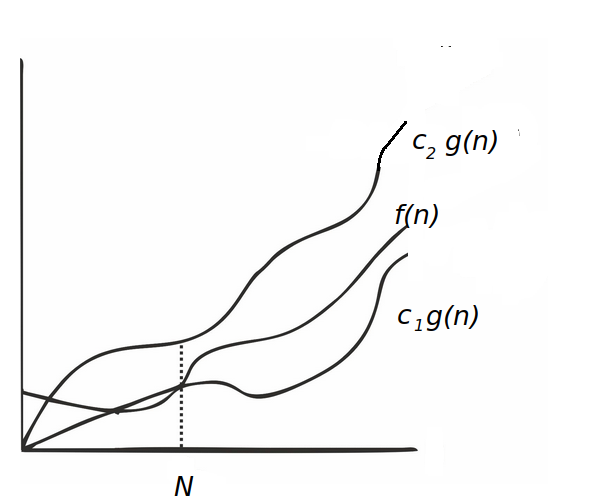
\includegraphics[width=170pt,height=150pt]{slike/theta-notation.png}
	\caption{$\Theta$--notacija: funkcija $f$ je ograničena odozgo i odozdo funkcijom $g$.}
	\label{fig:theta_notation}
\end{figure}

\begin{example}
	Vrijedi 	$T_1(n)=\Theta(n^{3/2}),$ 	dok je $T_2(n)=\Theta(n\log^3 n).$
\end{example}

Pored $O$ i $\Theta$ notacije, često se koriste i $\Omega$ i $o$ notacije.

\begin{definition}
	Neka su date funkcije $f$ i $g$. 	Kažemo da je 	$
	f(n)=\Omega(g(n))$   ako postoje konstante $c>0$ i $N>0$ takve da za svako $n\geq N$ važi $
	f(n)\geq c \cdot g(n).
	$	Funkcija $g$ tada predstavlja asimptotsku donju granicu funkcije $f$.
\end{definition}

\begin{example}
	Vrijedi 	$n^3=\Omega(n^2+n),$ kao i $
	n\log n=\Omega(n).$
\end{example}

\begin{definition}
	Neka su date funkcije $f$ i $g$.
	
	Kažemo da je $
	f(n)=o(g(n))$ ako za svako $c>0$ postoji broj $N>0$ takav da za svako $n\geq N$ važi $0\leq f(n)<c \cdot g(n).$ Drugim riječima, funkcija $f$ raste strogo sporije od funkcije $g$.
\end{definition}

Neformalno posmatrano, uslov $f(n)=o(g(n))
$ znači da odnos $
\frac{f(n)}{g(n)} $ teži nuli kada $n$ teži beskonačnosti.

\begin{example}
	Vrijedi $
	n=o(n^2),
	$ kao i 	$
	n=o(n^3).
	$ 	Međutim, 	$
	n\neq o(n).
	$
\end{example}

Asimptotske notacije predstavljaju osnovni jezik analize algoritama. Njihova najveća prednost ogleda se u tome što omogućavaju poređenje algoritama nezavisno od konkretne implementacije, programskog jezika ili hardverske platforme. Na taj način fokus se prebacuje na fundamentalno pitanje: kako vrijeme izvršavanja raste sa povećanjem veličine ulaza.


\subsection{Neka svojstva $O$--notacije}

Sljedeća teorema navodi nekoliko korisnih pravila koja se često koriste pri računanju asimptotske složenosti algoritama.

\begin{theorem}
	Neka su $f$, $g$ i $h$ pozitivne funkcije definisane za dovoljno velike vrijednosti argumenta. Tada vrijede sljedeće tvrdnje:
	
	\begin{itemize}
		\item $f = O(c \cdot f)$ za svako $c > 0$ \hfill (konstantni faktori su irelevantni);
		
		
		\item Ako je $f = O(g+h)$ i $h = O(g)$, tada je $f = O(g)$ \hfill (pravilo dominantnog člana);
		
		\item $O(f+g)=O(f)+O(g)$ \hfill (pravilo zbira);
		
		\item $O(f\cdot g)=O(f)\cdot O(g)$ \hfill (pravilo proizvoda);
		
		\item Ako je $f=O(g)$ i $g=O(h)$, tada je i $f=O(h)$ \hfill (pravilo tranzitivnosti).
		
		
	\end{itemize}
\end{theorem}

\begin{proof}
	Sve tvrdnje direktno slijede iz definicije $O$--notacije.
\end{proof}

\subsection{Uputstva za procjenu složenosti algoritama}

U prethodnoj sekciji uvedene su osnovne asimptotske notacije koje se koriste za procjenu složenosti algoritama. One omogućavaju da se vrijeme izvršavanja algoritma posmatra kao funkcija veličine ulaza, pri čemu se zanemaruju detalji koji ne utiču značajno na ponašanje algoritma za velike vrijednosti ulaza.

Najčešće funkcije koje se pojavljuju u analizi algoritama prikazane su u Tabeli~\ref{tab:slozenosti_funkcije-a}.

\begin{table}[H]
	\caption{Najčešće klase asimptotske složenosti.}
	\label{tab:slozenosti_funkcije-a}
	\centering
	\begin{tabular}{l|l}
		\hline
		\textbf{Funkcija} & \textbf{Klasa složenosti} \\
		\hline
		$1$ & konstantna  \\ \hline
		$\log n$ & logaritamska \\ \hline
		$n$ & linearna\\  \hline
		$n\log n$ & log-linearna \\ \hline
		$n^2$ & kvadratna \\ \hline
		$n^3$ & kubna \\ \hline
		$2^n$ & eksponencijalna \\ \hline
		$n!$ & faktorijelska \\ \hline
		\hline
	\end{tabular}
\end{table}

Rast navedenih funkcija u zavisnosti od veličine ulaza prikazan je na Slici~\ref{fig:slozenosti_funkcije-a}.

\begin{figure}[H]
	\centering
	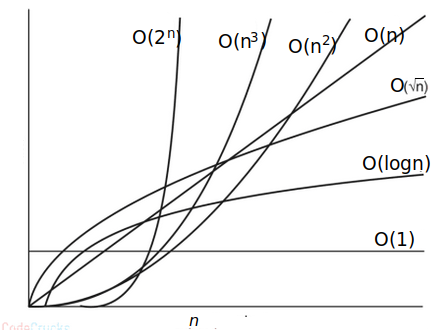
\includegraphics[width=170pt,height=130pt]{slike/growth.png}
	\caption{Poređenje najčešćih klasa složenosti.}
	\label{fig:slozenosti_funkcije-a}
\end{figure}

U praksi se algoritmi eksponencijalne i faktorijelske složenosti smatraju neefikasnim za ulaze velikih dimenzija, jer vrijeme njihovog izvršavanja veoma brzo raste sa povećanjem veličine ulaza. Sa druge strane, logaritamska, linearna i log-linearna složenost najčešće se smatraju poželjnim, budući da omogućavaju obradu veoma velikih instanci problema u razumnom vremenu.

Kvadratna složenost često predstavlja granicu praktične upotrebljivosti algoritma. Za neke probleme ona je sasvim prihvatljiva, dok za druge može biti nedovoljno efikasna, posebno kada se obrađuju veoma veliki skupovi podataka.

U nastavku navodimo nekoliko praktičnih pravila koja olakšavaju procjenu složenosti algoritama. Neka je sa $T(P)$ označena vremenska složenost programa ili programskog segmenta $P$.

\begin{table}[H]
	\caption{Pravila za procjenu složenosti algoritama.}
	\label{tab:uputstva_racunanje}
	\centering
	\begin{tabular}{l|l}
		\hline
		\textbf{Konstrukcija} & \textbf{Složenost} \\
		\hline
		Jedinična instrukcija & $1$ \\
		\hline
		$S: N_1; N_2$ & $T(S)=T(N_1)+T(N_2)$ \\
		\hline
		\textbf{IF} $C$ \textbf{THEN} $N_1$ \textbf{ELSE}  $N_2$ 
		& 
		$T(S)=T(C)+\max\{T(N_1),T(N_2)\}$ \\
		\hline
		\textbf{WHILE} $U$ \textbf{DO} $N_1$
		&
		$T(S)=n\cdot(T(U)+T(N_1))$ \
		\\ \hline
		\textbf{FOR} $i=j$ \textbf{TO} $p$ \textbf{DO} $N_1$
		&
		$T(S)=n\cdot T(N_1)$ \
		\\ \hline
	\end{tabular}
\end{table}

Pri procjeni složenosti algoritama najčešće se zanemaruju konstantni faktori i niži redovi rasta, a pažnja se usmjerava na dominantni član izraza. Na taj način moguće je brzo odrediti asimptotsko ponašanje algoritma bez potrebe za detaljnim brojanjem svih izvršenih instrukcija.\\

Postavlja se pitanje: kada možemo reći da je jedan algoritam efikasniji od drugog?\\


Odgovor daju upravo asimptotske notacije, prvenstveno $O$ i $\Theta$ notacija. Kažemo da je algoritam $X$ \textit{asimptotski efikasniji} od algoritma $Y$ ukoliko za dovoljno velike vrijednosti ulaza vrijeme izvršavanja algoritma $X$ raste sporije od vremena izvršavanja algoritma $Y$.

Drugim riječima, algoritam $X$ pripada nižoj klasi složenosti od algoritma $Y$. Na primjer, algoritam složenosti $O(n\log n)$ asimptotski je efikasniji od algoritma složenosti $O(n^2)$.

Važno je naglasiti da asimptotska efikasnost opisuje ponašanje algoritama za velike vrijednosti ulaza. Za male ulaze moguće je da algoritam sa lošijom asimptotskom složenošću bude brži zbog manjih konstantnih faktora ili jednostavnije implementacije. Ipak, kako veličina ulaza raste, prednost algoritma sa boljom asimptotskom složenošću postaje sve izraženija.


U narednom primjeru razmotrićemo jedan klasičan problem, prikazati dva različita algoritamska pristupa njegovom rješavanju i analizirati njihovu vremensku složenost.

\begin{example}(\textit{Problem podniza maksimalne sume})
	
	Dat je niz brojeva. Potrebno je odrediti neprekidni podniz početnog niza čija je suma elemenata najveća.
\end{example}

\begin{solution}
	
	Neka je dat niz $
	\texttt{a}=[1,4,-2,2,10,-7,1].
	$ 	Primjer jednog neprekidnog podniza jeste $[-2,2,10],$ 	dok niz $[-2,-7,1]$ nije neprekidan podniz jer njegovi elementi nisu uzastopni u izvornom nizu. 	Najprije razmotrimo naivan pristup. Definišimo funkciju
	
	$$
	S(i,j)=\sum_{k=i}^{j} a[k],
	$$
	
	pri čemu je $S(i,i)=a[i]$. 	Dakle, funkcija $S(i,j)$ predstavlja sumu elemenata neprekidnog podniza čiji su početni i završni indeks redom $i$ i $j$.
	
	Za izračunavanje vrijednosti $S(i,j)$ potrebno je sabrati $j-i+1$ elemenata, što zahtijeva $O(n)$ operacija u najgorem slučaju. 	Da bismo pronašli podniz maksimalne sume, potrebno je razmotriti sve moguće parove indeksa $(i,j)$ za koje važi $0 \leq i \leq j < n$. Broj takvih parova jednak je $
	\binom{n}{2}+n=\frac{n(n+1)}{2},
	$ što pripada klasi $O(n^2)$. Kako se za svaki od tih parova funkcija $S(i,j)$ računa u vremenu $O(n)$, ukupna složenost algoritma iznosi $
	O(n)\cdot O(n^2)=O(n^3).
	$	Dakle, dobijamo algoritam koji ima kubnu složenost.
	
	Pokušajmo sada konstruisati efikasniji pristup. Primijetimo da između vrijednosti $S(i,j)$ i $S(i,j+1)$ postoji jednostavna rekurzivna veza	$
	S(i,j+1)=S(i,j)+a[j+1].
	$
	
	Drugim riječima, ukoliko je suma podniza od pozicije $i$ do pozicije $j$ već poznata, suma narednog podniza može se dobiti dodavanjem samo jednog novog elementa. 	Definišimo 	
	$
	S(i)=\max\{S(i,i),S(i,i+1),\ldots,S(i,n-1)\}.$
	
	Vrijednost $S(i)$ može se izračunati prolaskom kroz niz počevši od pozicije $i$, pri čemu se tekuća suma ažurira u konstantnom vremenu. Zbog toga je složenost izračunavanja funkcije $S(i)$ jednaka $O(n)$.
	
	Pošto se funkcija $S(i)$ poziva za svaku početnu poziciju $i \in {0,\ldots,n-1}$, ukupna složenost algoritma iznosi 	$
	n \cdot O(n)=O(n^2).
	$ Time smo složenost smanjili sa $O(n^3)$ na $O(n^2)$, što predstavlja značajno poboljšanje u efikasnosti algoritma.
	
\end{solution}

\section{Prostorna složenost}

Pored vremena izvršavanja, važan kriterijum za procjenu kvaliteta algoritma jeste količina memorije koju algoritam koristi tokom rada.

Pri tome treba razlikovati pojmove \textit{pomoćni prostor} i \textit{prostorna složenost}. Pomoćni prostor predstavlja dodatnu memoriju koju algoritam koristi tokom izvršavanja, ne računajući prostor potreban za smještanje ulaznih podataka.  Sa druge strane, \textit{prostorna složenost} algoritma predstavlja ukupnu količinu memorije potrebne za njegovo izvršavanje, uključujući i prostor za ulazne podatke i pomoćne memorijske strukture.

Kao i kod vremenske složenosti, prostorna složenost izražava se kao funkcija veličine ulaza.  Na primjer:

\begin{itemize}
	\item kreiranje niza dužine $n$ zahtjeva $O(n)$ memorijskog prostora;
	\item kreiranje matrice dimenzija $n \times n$ zahtijeva $O(n^2)$ memorijskog prostora.
\end{itemize}

Efikasnost algoritma najčešće se procjenjuje na osnovu dva kriterijuma: vremena izvršavanja i količine korištene memorije. U mnogim situacijama postoji kompromis između ova dva resursa. Često je moguće ubrzati algoritam korišćenjem dodatne memorije, dok smanjenje memorijskih zahtijeva može dovesti do povećanja vremena izvršavanja.

\begin{example}
	Posmatrajmo sljedeće procedure.
	
	\begin{algorithm}[H]
		\begin{algorithmic}[1]
			\Procedure{pairSum}{x, y}
			\State \textbf{return} $x+y$
			\EndProcedure
		\end{algorithmic}
	\end{algorithm}
	
	\begin{algorithm}[H]
		\begin{algorithmic}[1]
			\Procedure{addSequence}{n}
			\State $sum \gets 0$
			
			\For{$i = 0$ \textbf{to} $n-1$}
			\State $sum \gets sum + \textsc{pairSum}(i,i+1)$
			\EndFor
			
			\State \textbf{return} $sum$
			\EndProcedure
		\end{algorithmic}
	\end{algorithm}
	
	Odredimo prostornu složenost procedure \textsc{AddSequence}.
	
	Iako se funkcija \textsc{pairSum} poziva $O(n)$ puta, ne dolazi do akumuliranja dodatnih memorijskih struktura. Tokom izvršavanja koristi se samo konstantan broj promjenljivih ($sum$, $i$, te parametri funkcije), pa je prostorna složenost algoritma jednaka	$
	O(1).
	$
	
	Drugim riječima, količina memorije ne zavisi od veličine ulaza $n$.
\end{example}

\textbf{Napomena.} 
U praktičnom programiranju raspoloživa memorija je ograničena. Na mnogim sistemima tipična memorijska ograničenja iznose između 128 MB i 512 MB po procesu. Zbog toga nije uvijek moguće kreirati veoma velike nizove ili matrice.

Takođe, lokalne promjenljive funkcija smještaju se na stek, čija je veličina obično znatno manja od ukupne raspoložive memorije procesa. Zbog toga se veoma velike strukture podataka često alociraju u globalnoj memoriji ili na hipu (eng. \emph{heap}), umjesto unutar tijela funkcije.

\section{Pseudok\^od}

\textit{Pseudokod} predstavlja neformalni način zapisivanja algoritama pomoću kombinacije prirodnog jezika i programerskih konstrukcija. Njegova svrha nije da bude izvršiv na računaru, već da na jasan i nedvosmislen način predstavi logiku algoritma.

Za razliku od programskog k\^oda, pseudok\^od ne posjeduje strogo definisanu sintaksu i ne može se kompajlirati niti interpretirati. Upravo zbog toga omogućava da se pažnja usmjeri na suštinu algoritma, bez opterećivanja detaljima konkretnog programskog jezika.

Pseudok\^od predstavlja koristan međukorak između ideje rješenja i njegove implementacije. Njime se opisuje redoslijed koraka koje je potrebno izvršiti kako bi se riješio određeni problem, pri čemu zapis ostaje dovoljno prost da ga mogu razumjeti i osobe koje nisu upoznate sa svim detaljima implementacije.

Prednosti korišćenja pseudok\^oda su višestruke:

\begin{itemize}
	\item Poboljšava čitljivost i razumijevanje algoritma.
	
	\item Omogućava fokusiranje na logiku rješenja umjesto na sintaksu programskog jezika.
	
	\item Predstavlja prirodnu vezu između idejnog rješenja, dijagrama toka i implementacije.
	
	\item Služi kao oblik dokumentacije koji olakšava kasnije održavanje i unapre\-đivanje programa.
	
\end{itemize}

Osnovni cilj pseudokoda jeste da nedvosmisleno opiše svaki korak algoritma. Time se olakšava implementacija i smanjuje vjerovatnoća nastanka grešaka tokom razvoja programa.

Konstrukcija pseudokoda započinje detaljnim razumijevanjem problema koji se rješava. Nakon identifikacije potrebnih koraka, koraci se zapisuju u obliku jednostavnih i jasno formulisanih instrukcija.

Prilikom pisanja pseudokoda preporučuje se pridržavanje sljedećih smjernica:

\begin{itemize}
	\item Koristiti jasne i opisne nazive promjenljivih i funkcija.
	
	\item Svaki korak algoritma opisati dovoljno precizno da ne postoji mogućnost različitog tumačenja.
	
	\item Posebnu pažnju posvetiti uslovima zaustavljanja algoritma.
	
	\item Jasno naglasiti strukturu grananja i petlji korišćenjem uvlačenja naredbi.
	
	\item Izbjegavati nepotrebne implementacione detalje i zadržati fokus na logici rješenja.
	
\end{itemize}

Primjer jednostavnog pseudokoda:

\begin{minted}{text}
	tip = unos sa tastature
	
	ako je tip = "1"
	ispiši "Unesen je broj 1"
	
	ako je tip = "2"
	ispiši "Unesen je broj 2"
\end{minted}

Primijetimo da ovakav zapis ne predstavlja program u konkretnom programskom jeziku, već opisuje logiku koju bi program trebalo da realizuje.

\begin{example}
	Napisati pseudokod za pronalaženje najvećeg elementa niza.
	
	\begin{minted}{text}
		Postavi najveći element na prvi element niza.
		
		Prolazi kroz elemente niza jedan po jedan.
		
		Ako je trenutni element veći od najvećeg do sada 
	        pronađenog,
		    ažuriraj vrijednost najvećeg elementa.
		Kraj prolaska kroz niz.
		
		Prikaži najveći element.
	\end{minted}
	
\end{example}

U nastavku prikazujemo formalniji oblik pseudok\^oda, kakav se često koristi u literaturi iz algoritama. Posmatrajmo algoritam za rješavanje problema podniza maksimalne sume iz prethodne sekcije.

\begin{algorithm}[!ht]
	\caption{Funkcija $S_i(i)$}
	\label{S_i}
	\begin{algorithmic}[1]
		\Procedure{$S_i$}{$i$, $niz$}

		\State $s_{\max} \gets niz[i]$
		\State $s \gets niz[i]$
		
		\For{$j=i+1$ to $n-1$}
		\State $s \gets s + niz[j]$
		
		\If{$s > s_{\max}$}
		\State $s_{\max} \gets s$
		\EndIf
		
		\EndFor
		
		\State \Return $s_{\max}$
		
		\EndProcedure
	\end{algorithmic}
\end{algorithm}

\begin{algorithm}[H]
	\caption{Funkcija $S$}
	\label{S}
	\begin{algorithmic}[1]
		\Procedure{$S$}{$niz$}
		\State $s_{\max} \gets niz[0]$
		
		\For{$i=0$ to $n-1$}
		
		\State $s_i \gets S_i(i,niz)$
		
		\If{$s_i > s_{\max}$}
		\State $s_{\max} \gets s_i$
		\EndIf
		
		\EndFor
		
		\State \Return $s_{\max}$
		
		\EndProcedure
	\end{algorithmic}
\end{algorithm}

Ovakav način zapisivanja pseudokoda predstavlja standard u većini udžbenika i naučnih radova iz oblasti algoritama. Iako je formalniji od prethodnih primjera, i dalje ostaje nezavisan od konkretnog programskog jezika, što omogućava da se algoritam jednostavno implementira u Pajtonu, Javi, C-u, C++-u ili bilo kojem drugom jeziku.

\section{O valjanosti algoritma}

Pored analize vremenske i prostorne složenosti, važno je pokazati da algoritam zaista rješava problem za koji je konstruisan. Drugim riječima, potrebno je dokazati njegovu \textit{valjanost} (ispravnost).

Postoji više pristupa dokazivanju ispravnosti algoritama, među kojima izdvajamo sljedeće:

\begin{itemize}
	\item \textit{Matematički dokaz}. Predstavlja najrigorozniji pristup dokazivanju ispravnosti algoritma. Cilj je pokazati da algoritam za svaki dopustiv ulaz vraća ispravno rješenje problema. Jedna od najčešće korištenih tehnika jeste metoda \textit{invarijante petlje}, koju ćemo razmotriti u nastavku.
	
	\item \textit{Formalna verifikacija}. Podrazumijeva modelovanje algoritma pomoću formalnog jezika i korištenje specijalizovanih alata za automatsku provjeru željenih svojstava. Ovakve metode imaju značajnu primjenu u razvoju kritičnih softverskih sistema, gdje čak i mala greška može imati ozbiljne posljedice.
	
	\item \textit{Testiranje}. Iako ne predstavlja formalni dokaz ispravnosti, testiranje je nezaobilazan korak u razvoju softvera. Pokretanjem algoritma nad velikim brojem pažljivo odabranih testnih primjera može se steći visok stepen povjerenja u njegovu ispravnost.
	
\end{itemize}

%\subsection{Metoda invarijante petlje}

Metoda \textit{invarijante petlje} predstavlja jednu od najvažnijih tehnika za dokazivanje ispravnosti iterativnih algoritama.

\begin{definition}
	Invarijanta petlje je tvrđenje koje važi prije prve iteracije petlje, ostaje tačno nakon svake iteracije i važi u trenutku završetka petlje.
\end{definition}

Dokaz ispravnosti algoritma pomoću invarijante petlje obično se sastoji od tri koraka:

\begin{enumerate}
	\item \textbf{Inicijalizacija}. Pokazuje se da invarijanta važi prije prve iteracije petlje.
	
	\item \textbf{Održavanje}. Dokazuje se da, ukoliko invarijanta važi prije određene iteracije, ona ostaje tačna i nakon izvršavanja te iteracije.
	
	\item \textbf{Završetak}. Nakon izlaska iz petlje koristi se invarijanta kako bi se pokazalo da rezultat koji algoritam vraća zaista predstavlja rješenje problema.
	
\end{enumerate}

Prednost ove metode ogleda se u tome što omogućava formalno dokazivanje ispravnosti algoritama koji koriste petlje, bez potrebe da se zasebno analiziraju svi mogući ulazi.

\begin{example}
	Razmotrimo sljedeći algoritam za određivanje najvećeg zajedničkog djelioca (NZD) dva prirodna broja.
\end{example}

\begin{algorithm}[H]
	\begin{algorithmic}[1]
		\Procedure{NZD}{$n,m$}
		\State $d \gets \min(n,m)$
		\While{$n \bmod d \neq 0$ \textbf{or} $m \bmod d \neq 0$}
		\State $d \gets d-1$
		\EndWhile
		
		\State \Return $d$
		\EndProcedure
	\end{algorithmic}
	\caption{Naivni algoritam za određivanje NZD-a.}
	\label{alg:nzd}
	
\end{algorithm}

Neka je sa $d^*$ označen najveći zajednički djelilac brojeva $n$ i $m$. Posmatrajmo tvrđenje $
d^* \leq d.
$  Pokazaćemo da ono predstavlja invarijantu petlje.

\begin{itemize}
	\item \textbf{Inicijalizacija.} Prije prve iteracije važi $
	d=\min(n,m).
	$
	
	Pošto najveći zajednički djelilac ne može biti veći od manjeg od dva broja, slijedi da je 	$
	d^* \leq d.
	$   Dakle, invarijanta važi prije ulaska u petlju.
	
	\item \textbf{Održavanje.} Pretpostavimo da invarijanta važi na početku neke iteracije. U tijelu petlje vrijednost promjenljive $d$ smanjuje se za jedan.
	
	Sve dok se petlja izvršava, trenutna vrijednost $d$ nije zajednički djelilac oba broja. Budući da je $d^*$ najveći zajednički djelilac, mora važiti 	$
	d^* < d.
	$
	
	Nakon izvršavanja naredbe $d \gets d-1$ i dalje ostaje 	$
	d^* \leq d,
	$ pa je invarijanta očuvana.
	
	\item \textbf{Završetak.} Petlja se zaustavlja kada trenutna vrijednost $d$ dijeli i broj $n$ i broj $m$. Dakle, tada je $d$ zajednički djelilac. 	S druge strane, prema invarijanti petlje važi $
	d^* \leq d.
	$
	
	Pošto algoritam ispituje kandidate silaznim redoslijedom, prvi pronađeni zajednički djelilac mora biti upravo najveći zajednički djelilac. Dakle, 	$
	d=d^*.
	$
\end{itemize}

Time je pokazano da algoritam zaista vraća najveći zajednički djelilac ulaznih brojeva.


U praksi je pronalaženje odgovarajuće invarijante često najzahtjevniji dio dokaza. Kod složenijih algoritama invarijanta može biti veoma komplikovana, pa formalni dokaz postaje težak za izvođenje i razumijevanje. Zbog toga se u razvoju softvera formalni dokazi često kombinuju sa opsežnim testiranjem i empirijskom provjerom ispravnosti.

\section{Euklidov algoritam}

Jedan od najstarijih i najpoznatijih algoritama u matematici jeste \textit{Euklidov algoritam} za određivanje najvećeg zajedničkog djelioca (NZD) dva prirodna broja. Algoritam je dobio ime po starogrčkom matematičaru Euklidu, koji ga je opisao u djelu \textit{Elementi} prije više od dvije hiljade godina.

Osnovna ideja algoritma zasniva se na sljedećem svojstvu:

$$\text{NZD}(a,b)=\text{NZD}(b,a\bmod b).$$

Drugim riječima, najveći zajednički djelilac brojeva $a$ i $b$ jednak je najvećem zajedničkom djeliocu brojeva $b$ i ostatka pri dijeljenju broja $a$ brojem $b$. Ovo svojstvo omogućava da se problem postepeno svodi na manje ulaze, sve dok jedan od tih ulaza ne dobije vrijednost nula.

\begin{algorithm}[H]
	\begin{algorithmic}[1]
		\Procedure{NZD}{$a,b$}
		\While{$b \neq 0$}
		\State $r \gets a \bmod b$
		\State $a \gets b$
		\State $b \gets r$
		\EndWhile
		\State \Return $a$
		\EndProcedure
	\end{algorithmic}
	\caption{Euklidov algoritam.}
	\label{alg:nzd-euclid}
\end{algorithm}

\begin{example}
	
	Odredimo najveći zajednički djelilac brojeva 	$
	a=400$ i $b=24.$ 
\end{example}
	
	\begin{solution}
	Algoritam izvršava sljedeće transformacije: 	$
	(400,24)
	\rightarrow
	(24,16)
	\rightarrow
	(16,8)
	\rightarrow
	(8,0).
	$	Pošto je u posljednjem koraku drugi broj jednak nuli, algoritam se zaustavlja i vraća vrijednost prvog broja. Dakle, $\text{NZD}(400,24)=8.$
\end{solution}


Za razliku od naivnog algoritma iz prethodne sekcije, koji u najgorem slučaju ispituje sve brojeve od $\min(a,b)$ do $1$, Euklidov algoritam veoma brzo smanjuje vrijednosti brojeva nad kojima radi. Zbog toga se u praksi koristi gotovo isključivo Euklidov pristup.

Može se pokazati da broj iteracija Euklidovog algoritma raste proporcionalno logaritmu manjeg od ulaznih brojeva. Preciznije, broj iteracija pripada klasi $O(\log \min(a,b)).$

Pri analizi algoritama često se veličina ulaza ne mjeri samim brojevima $a$ i $b$, već brojem bitova potrebnih za njihov zapis. Ako sa $n$ označimo ukupan broj bitova potrebnih za predstavljanje ulaznih brojeva, tada približno važi $
n \approx \log_2(a)+\log_2(b).
$ Prema tome, broj iteracija algoritma raste linearno u odnosu na veličinu ulaza izraženu u bitovima, odnosno pripada klasi $O(n).
$ Pored male vremenske složenosti, Euklidov algoritam koristi svega nekoliko pomoćnih promjenljivih ($a$, $b$ i $r$), pa je njegova prostorna složenost jednaka $O(1).
$

Zahvaljujući svojoj jednostavnosti i efikasnosti, Euklidov algoritam predstavlja jedan od najvažnijih algoritama u teoriji brojeva i računarstvu. Njegove modifikacije koriste se u brojnim oblastima, uključujući kriptografiju, računarsku algebru i teoriju algoritama.

\textbf{Napomena.}
Valjanost Euklidovog algoritma direktno slijedi iz svojstva $\text{NZD}(a,b)=\text{NZD}(b,a\bmod b),$ koje se primjenjuje u svakoj iteraciji algoritma. Budući da se vrijednost drugog argumenta strogo smanjuje, algoritam se nakon konačnog broja koraka zaustavlja, a posljednja nenulta vrijednost predstavlja najveći zajednički djelilac ulaznih brojeva.

\section{Master teorema}

Kod analize algoritama veoma često se pojavljuju rekurzivne relacije koje opisuju
vrijeme izvršavanja algoritma. Ovakve relacije su naročito karakteristične za
algoritamske paradigme zasnovane na rekurzivnom principu, kao što je paradigma
\emph{podijeli pa zavladaj}.

Pretpostavimo da algoritam problem veličine $n$ dijeli na $a$ podproblema,
pri čemu svaki podproblem ima veličinu približno $n/b$. Pored vremena potrebnog
za rješavanje podproblema, algoritam troši dodatno vrijeme za podjelu problema,
kombinovanje parcijalnih rješenja ili druge operacije. Tada se vremenska
složenost algoritma često može opisati rekurentnom relacijom oblika

\[
T(n)=aT\left(\frac{n}{b}\right)+f(n),
\]

gdje je:

\begin{itemize}
	\item $a \geq 1$ broj podproblema koji se rekurzivno rješavaju;
	\item $b > 1$ faktor za koji se smanjuje veličina svakog podproblema;
	\item $f(n)$ vrijeme potrebno za operacije koje se izvršavaju izvan
	rekurzivnih poziva, kao što su podjela problema ili kombinovanje rješenja.
\end{itemize}

Određivanje asimptotske složenosti ovakvih rekurentnih relacija može biti
zahtjevno. \emph{Master teorema} daje jednostavan način za određivanje
asimptotske složenosti velikog broja rekurzija ovog tipa.

\begin{theorem}[Master teorema]
	Neka je vremenska složenost algoritma opisana relacijom
	
	\[
	T(n)=aT\left(\frac{n}{b}\right)+f(n),
	\]
	
	gdje su $a\geq 1$ i $b>1$ konstante. Vrijednost
	
	\[
	n^{\log_b a}
	\]
	
	predstavlja osnovnu veličinu sa kojom se poredi funkcija $f(n)$.
	
	Tada, u najčešćim slučajevima, vrijedi:
	
	\begin{enumerate}
		\item Ako funkcija $f(n)$ raste asimptotski sporije od
		$n^{\log_b a}$, tada je
		
		\[
		T(n)=\Theta\left(n^{\log_b a}\right).
		\]
		
		\item Ako funkcija $f(n)$ raste istom asimptotskom brzinom kao
		$n^{\log_b a}$, tada je
		
		\[
		T(n)=\Theta\left(n^{\log_b a}\log n\right).
		\]
		
		\item Ako funkcija $f(n)$ raste asimptotski brže od
		$n^{\log_b a}$, tada je, pod odgovarajućim dodatnim uslovima,
		
		\[
		T(n)=\Theta(f(n)).
		\]
	\end{enumerate}
\end{theorem}

Drugim riječima, osnovna ideja Master teoreme jeste poređenje troška
rekurzivnih poziva sa troškom operacija koje se izvršavaju izvan rekurzije.

\begin{example}
	 Neka je data rekurzija
	\[
	T(n)=T\left(\frac{n}{2}\right)+\Theta(1).
	\]
	
	Ovdje je $a=1$, $b=2$ i $f(n)=\Theta(1)$. Pošto je
	
	\[
	n^{\log_2 1}=n^0=1,
	\]
	
	funkcija $f(n)$ ima isti red rasta kao $n^{\log_b a}$. Primjenom drugog
	slučaja Master teoreme dobijamo
	
	\[
	T(n)=\Theta(\log n).
	\]
	
	Dakle, vremenska složenost binarne pretrage je logaritamska.
\end{example}

\begin{example}
%	Kod algoritma sortiranja spajanjem (\emph{merge sort}) niz se dijeli na dva
%	podniza približno jednake veličine. Oba podniza se rekurzivno sortiraju, dok
%	operacija njihovog spajanja zahtijeva linearno vrijeme. 
Neka je data rekurentna relacija
	
	\[
	T(n)=2T\left(\frac{n}{2}\right)+\Theta(n).
	\]
	
	U ovom slučaju je $a=2$, $b=2$ i
	
	\[
	n^{\log_2 2}=n.
	\]
	
	Pošto je $f(n)=\Theta(n)$, primjenjuje se drugi slučaj Master teoreme, pa je
	
	\[
	T(n)=\Theta(n\log n).
	\]
\end{example}

\begin{example}
	%Kod Karacubinog algoritma za množenje cijelih brojeva pojavljuje se rekurzija
	U slučaju rekurzicne relacije
	\[
	T(n)=3T\left(\frac{n}{2}\right)+\Theta(n).
	\]
	
	imamo $a=3$ i $b=2$, pa je
	
	\[
	n^{\log_2 3}\approx n^{1.585}.
	\]
	
	Kako funkcija $n$ raste sporije od $n^{\log_2 3}$, primjenjuje se prvi slučaj
	Master teoreme. Prema tome,
	
	\[
	T(n)=\Theta\left(n^{\log_2 3}\right)
	\approx \Theta\left(n^{1.585}\right).
	\]
\end{example}

Master teorema predstavlja veoma koristan alat za brzu procjenu vremenske
složenosti algoritama zasnovanih na rekurzivnom razlaganju problema. U ovoj
knjizi koristićemo je prvenstveno za analizu jednostavnih algoritama zasnovanih
na paradigmi podijeli pa zavladaj.

Detaljan dokaz Master teoreme, njene preciznije formulacije, dodatni uslovi
primjene i slučajevi koji nisu obuhvaćeni prethodno navedenim pravilima
obrađuju se na naprednijim kursevima iz algoritama i analize algoritama na
višim godinama studija.



\section*{Zadaci}

\begin{enumerate}
	\item Izračunati vremensku složenost sljedećeg programa:
	
	\begin{algorithm}[H]
		\begin{algorithmic}[1]
		\Procedure{Zad1}{$N$}
		    \State $ a \gets  0$
		    \For{$i = 0 \text{ to } N$}
		         \For{$j = N \text{ downto } i$}
		    		\State $a \gets  a + i + j$
		         \EndFor
		     \EndFor
	    \EndProcedure	 	    
		\end{algorithmic}
	\end{algorithm}
\item Izračunati vremensku složenost sljedećeg programa 
	\begin{algorithm}[H]
	\begin{algorithmic}[1]
	 \Procedure{Zad2}{$n$}
		\State $i, j, k \gets  0$
		\For{$i = n / 2 \text{ to } n$}
			\For{$j = 2; j \leq n; j = j * 2$}
				\State $k \gets  k + n / 2$
			\EndFor
		\EndFor
	\EndProcedure	 
	\end{algorithmic}
\end{algorithm}
 \item Izračunati vremensku složenost sljedećeg programa 

	\begin{algorithm}[H]
	\begin{algorithmic}[1]
     \Procedure{Zad3}{$N$}
		\State $a \gets 0, i \gets N$
		\While{$i > 0$}
			\State $a \gets a+ i$
			\State $i \gets i / 2$
		\EndWhile
    \EndProcedure	 
	\end{algorithmic}
\end{algorithm}
 \item Izračunati vremensku složenost sljedećeg programa 

\begin{algorithm}[H]
	\begin{algorithmic}[1]
	 \Procedure{Zad4}{$n$}
		\State $k \gets 3$
		\For{$i=0 \text{ to } n-1$}
		    \State $i \gets i * k$
		\EndFor
	   \EndProcedure
	\end{algorithmic}
\end{algorithm}

 \item Izračunati vremensku složenost sljedećeg programa 

\begin{algorithm}[H]
	\begin{algorithmic}[1]
	\Procedure{Zad5}{$n$}
	  \State $sum \gets 0$
	  \For{$i = 1 \text{ to } n$}
	      \For{$j = 1 \text{ to } i\cdot i$}
	          \If{$j \text{ mod } i == 0$}
	              \For{ $k = 1 \text{ to } j$}
                      \State	$sum \gets sum + 1$
                 
                  \EndFor
              \EndIf
          \EndFor
     \EndFor
    \EndProcedure
	\end{algorithmic}
\end{algorithm}


 
 \item Izračunati (ukupnu) složenost sljedeće rekurzije:

\begin{algorithm}[H]
	\begin{algorithmic}[1]
		\Procedure{bubbleSort}{$arr[],size$}
        \For{$i = 0; i < size-1; ++i$}
 	        \For{$j = 0; j < size-1; ++j$}
 	  
 	 	      \If{$arr[j] > arr[j+1]$}
 		        \State $swap( arr [j] , arr [j+1] )$
 		      \EndIf
 		   \EndFor
 	    \EndFor
		\EndProcedure
	\end{algorithmic}
\end{algorithm}



 
	 
 \item Izračunati složenost sljedeće rekurzije: %https://www.geeksforgeeks.org/analysis-algorithms-set-5-practice-problems/?ref=rp
  
 $$	T(n) = 
 \begin{cases}    
         &3\cdot T(n-1), \text{ako }  n > 0 , \\
         & 1, \text{inače} 
   \end{cases}$$

  \item Izračunati složenost sljedeće rekurzije:

$$	T(n) = 
\begin{cases} 
  		&2T(n-1) - 1, \text{ako } n>0, \\
		& 1, \text{inače}
\end{cases}
$$

\item Izračunati prostornu složenost programa datog sljedećim pseudokodom
%https://www.prepbytes.com/blog/data-structure/space-complexity/

\begin{algorithm}[H]
	\begin{algorithmic}[1]
		\Procedure{sum}{$arr[],N$}
		
		\State  $ans \gets 0$
		\For{$i = 0 \text{ to } N$}
		\State $ans \gets ans+arr[i]$
		\EndFor
		\State ispiši $ans$
		\EndProcedure
	\end{algorithmic}
\end{algorithm}



\item Izračunati prostornu složenost programa datog sljedećim pseudokodom
%https://www.prepbytes.com/blog/data-structure/space-complexity/
 
\begin{algorithm}[H]
	\begin{algorithmic}[1]
	  \Procedure{faktorijel}{$N$}
	  	\State $fact \gets 1$
	  	 \For{$i=1 \text{ to } N $}
	  	   
	  	   \State	$fact \gets fact * i$
	  	 \EndFor
	  	\State \textbf{return} \textit{fact}
	  \EndProcedure
	\end{algorithmic}
\end{algorithm}
 


\end{enumerate}
\chapter{Uvod u programski jezik Pajton}

Pajton (\textit{Python}) je interpretirani, objektno-orijentisani programski jezik visokog nivoa opšte namjene. Razvio ga je holandski programer Guido van Rossum, a prva javna verzija jezika objavljena je u februaru 1991. godine. Naziv jezika potiče od britanske humorističke grupe \textit{Monty Python}, čiji je rad inspirisao autora tokom razvoja jezika.

Od svog nastanka Pajton je prošao kroz više razvojnih faza i danas predstavlja jedan od najrasprostranjenijih programskih jezika u akademskom i industrijskom okruženju. Njegova popularnost rezultat je prije svega jednostavne sintakse, velike čitljivosti koda i bogatog ekosistema biblioteka koje omogućavaju primjenu jezika u različitim oblastima. Pregled popularnosti programskih jezika prikazan je na Slici~\ref{fig: popular_program_lang}\footnote{Preuzeto sa {https://www.tiobe.com/tiobe-index/}}.

\begin{figure}[H]
	\centering
	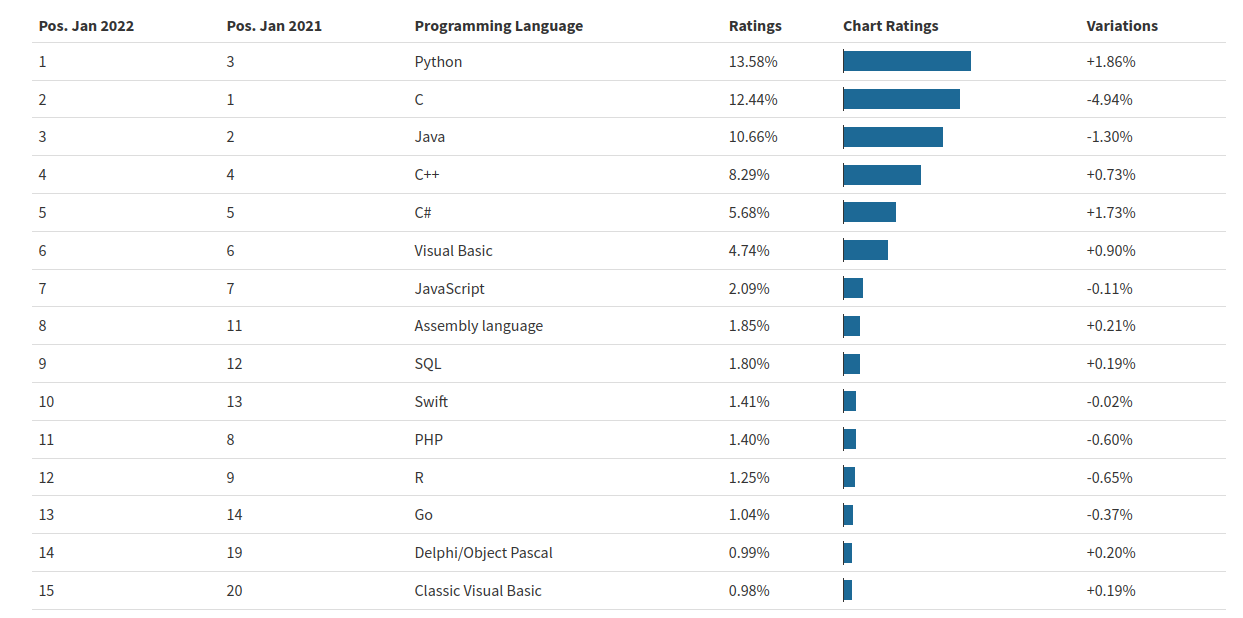
\includegraphics[width=400pt,height=190pt]{slike/most_popular_language.png}
	\caption{Statistički pregled najpopularnijih programskih jezika (2021--2022)}
	\label{fig: popular_program_lang}
\end{figure}

Početak razvoja Pajtona vezuje se za 1989. godinu, kada je Guido van Rossum započeo rad na novom programskom jeziku inspirisanom jezikom ABC. Cilj je bio kreiranje jezika koji bi zadržao jednostavnost i preglednost ABC-a, ali istovremeno pružio veću fleksibilnost i mogućnosti za razvoj složenijih softverskih sistema.

Prva verzija jezika, Pajton 0.9.0, objavljena je 1991. godine. Već tada su bili prisutni brojni koncepti koji i danas predstavljaju osnovu jezika, uključujući funkcije, klase, izuzetke i module.

Pajton 1.0 objavljen je 1994. godine i donio je dodatne funkcionalnosti inspirisane funkcionalnim programiranjem, kao što su funkcije \texttt{map}, \texttt{filter}, \texttt{reduce} i lambda izrazi. Verzija 2.0, objavljena 2000. godine, uvela je značajna unapređenja poput komprehenzije lista (\textit{list comprehensions}) i automatskog upravljanja memorijom putem sakupljača otpadaka (\textit{garbage collector}).

Velika prekretnica u razvoju jezika dogodila se 2008. godine objavljivanjem verzije Pajton 3.0. Ova verzija donijela je niz izmjena koje nisu bile u potpunosti kompatibilne sa prethodnim verzijama jezika, ali su omogućile jednostavniji, konzistentniji i pregledniji dizajn. Sve savremene verzije Pajtona zasnovane su na grani Pajton 3.

Danas se Pajton koristi u velikom broju oblasti, uključujući:

\begin{itemize}
	\item razvoj veb aplikacija;
	\item naučno i numeričko računarstvo;
	\item obradu i analizu podataka;
	\item mašinsko učenje i vještačku inteligenciju;
	\item automatizaciju zadataka i sistemsko programiranje;
	\item razvoj obrazovnog softvera.
\end{itemize}

Veliki doprinos popularnosti jezika daje i njegova izuzetno aktivna zajednica korisnika i programera. Tokom godina razvijen je veliki broj biblioteka i razvojnih okruženja koja značajno proširuju mogućnosti jezika. Među najpoznatijim bibliotekama nalaze se NumPy, Pandas, Matplotlib, SciPy, TensorFlow i PyTorch, dok su Django i Flask među najpopularnijim okvirima za razvoj veb aplikacija.

Pajton se posebno ističe jednostavnošću sintakse i čitljivošću programskog koda. Za razliku od mnogih drugih programskih jezika, naglasak je stavljen na preglednost i jasnoću programa, zbog čega se često preporučuje kao prvi programski jezik za učenje programiranja. Istovremeno, njegova izražajnost i bogat skup biblioteka čine ga pogodnim i za razvoj složenih profesionalnih softverskih sistema.

U ovoj knjizi Pajton će biti korišćen kao alat za implementaciju i eksperimentisanje sa različitim algoritamskim tehnikama. Njegova jednostavna sintaksa omogućava da se pažnja usmjeri na razumijevanje algoritama i struktura podataka, a ne na tehničke detalje implementacije karakteristične za jezike nižeg nivoa.\\

%ISHODI UCENJA:

Nakon uspješnog savladavanja sadržaja ove glave student će biti u stanju da:

\begin{itemize}
	\item objasni osnovne karakteristike programskog jezika Pajton i
	način predstavljanja podataka u memoriji;
	
	\item koristi osnovne numeričke i složene tipove podataka, uključujući
	stringove, liste, nizove, rječnike, skupove i torke;
	
	\item primijeni uslovne naredbe i petlje pri implementaciji
	jednostavnih proceduralnih algoritama;
	
	\item definiše i koristi funkcije, parametre, povratne vrijednosti i
	ugrađene funkcionalnosti za obradu kolekcija podataka;
	
	\item organizuje programski kod korištenjem modula i koristi odabrane
	module standardne biblioteke i eksternih biblioteka;
	
	\item prepoznaje, generiše i obrađuje izuzetke te koristi mehanizme za
	provjeru ispravnosti izvršavanja programa;
	
	\item koristi datoteke,  regularne izraze za učitavanje,
	obradu i zapisivanje strukturiranih podataka;
	
	\item objasni osnovne faze izvršavanja Pajton programa, uključujući
	generisanje bajtkoda, ulogu virtuelne mašine i osnovne principe
	upravljanja memorijom.
\end{itemize}

\section{Osnovne karakteristike}

Pajton posjeduje niz osobina koje ga čine pogodnim kako za učenje programiranja, tako i za razvoj složenih softverskih sistema. U nastavku navodimo njegove najvažnije karakteristike.

\begin{itemize}
	\item \textit{Jezik visokog nivoa} (\textit{high-level language}). Pajton omogućava programiranje na visokom nivou apstrakcije, pri čemu se programer može fokusirati na rješavanje problema, a ne na detalje rada računara. Sintaksa jezika je jednostavna i pregledna, zbog čega je k\^od relativno lako čitati i održavati.
	
	\item \textit{Dinamički tipiziran jezik}. Tip promjenljive određuje se tokom izvršavanja programa. Zbog toga nije potrebno unaprijed deklarisati tip svake promjenljive. Na primjer, ista promjenljiva može u jednom trenutku sadržavati cijeli broj, a kasnije tekstualnu vrijednost.
	
	\item \textit{Objektno-orijentisani jezik}. U Pajtonu su podaci i operacije nad njima organizovani kroz objekte i klase. Objektno-orijentisano programiranje omogućava modelovanje problema pomoću objekata i njihovih međusobnih interakcija, što često dovodi do preglednijeg i modularnijeg koda.
	
	\item \textit{Interpretirani i skriptni jezik}. Programi napisani u Pajtonu izvršavaju se posredstvom interpretera, bez potrebe za klasičnim procesom kompajliranja kakav postoji kod jezika poput C ili C++. Zbog toga je razvoj programa brz i pogodan za automatizaciju različitih zadataka.
	
	\item \textit{Automatsko upravljanje memorijom}. Pajton posjeduje ugrađene mehanizme za automatsko oslobađanje memorije koja više nije potrebna programu (\textit{garbage collection}). Time se značajno smanjuje mogućnost grešaka povezanih sa ručnim upravljanjem memorijom.

\end{itemize}

Zahvaljujući ovim karakteristikama, Pajton se danas koristi u obrazovanju, naučnim istraživanjima, analizi podataka, vještačkoj inteligenciji, razvoju veb aplikacija i mnogim drugim oblastima.

\section{Pregled ugrađenih tipova podataka}

Pajton posjeduje veliki broj ugrađenih (\textit{built-in}) tipova podataka koji su dostupni bez potrebe za instalacijom dodatnih biblioteka. Svaki tip podataka definiše način predstavljanja i manipulacije određenom vrstom informacija.

Najvažniji ugrađeni tipovi podataka su:

\begin{itemize}
	\item numerički tipovi: \texttt{int}, \texttt{float}, \texttt{complex};
	
	```
	\item tekstualni tipovi: \texttt{str};
	
	\item sekvencijalni tipovi: \texttt{list}, \texttt{tuple}, \texttt{range};
	
	\item mapirajući tipovi: \texttt{dict};
	
	\item skupovni tipovi: \texttt{set}, \texttt{frozenset};
	
	\item logički tip: \texttt{bool};
	
	\item binarni tipovi: \texttt{bytes}, \texttt{bytearray}, \texttt{memoryview}.
	```
	
\end{itemize}

Ovi tipovi predstavljaju osnovu za izgradnju složenijih struktura podataka i implementaciju različitih algoritama. U nastavku poglavlja detaljno ćemo razmotriti najvažnije od njih.

\section{Deklarisanje varijabli i memorijska organizacija}

Promjenljive u Pajtonu kreiraju se dodjelom vrijednosti pomoću operatora dodjele \texttt{=}.

Za razliku od mnogih drugih programskih jezika, nije potrebno unaprijed deklarisati tip promjenljive. Pajton automatski određuje odgovarajući tip na osnovu dodijeljene vrijednosti.

Na primjer, promjenljiva \texttt{x} kojoj se dodjeljuje cijeli broj 5 kreira se na sljedeći način:

\begin{minted}{python}
	x = 5
\end{minted}

Slično tome, promjenljivoj \texttt{y} možemo dodijeliti tekstualnu vrijednost:

\begin{minted}{python}
	y = "abc"
\end{minted}

Prilikom izvršavanja programa Pajton kreira odgovarajuće objekte u memoriji, dok promjenljive predstavljaju reference na te objekte. Zbog toga promjenljiva ne sadrži nužno samu vrijednost, već informaciju o tome gdje se odgovarajući objekat nalazi u memoriji.

U narednim sekcijama detaljnije ćemo razmotriti numeričke, tekstualne i složene tipove podataka, kao i način njihovog korištenja u programima.

 Pajton je objektno-orijentisani programski jezik, što znači da se sve vrijednosti u programu predstavljaju kao objekti. Drugim riječima, svaka promjenljiva zapravo referencira neki objekat smješten u memoriji.
 
 Na primjer, promjenljiva koja sadrži cijeli broj predstavlja referencu na objekat tipa \texttt{int}, dok promjenljiva koja sadrži tekst predstavlja referencu na objekat tipa \texttt{str}. U tom smislu, promjenljive u Pajtonu ne čuvaju direktno vrijednosti, već reference na objekte koji sadrže te vrijednosti.
 
 Posmatrajmo sljedeći primjer:
 
 \begin{minted}{python}
 	x = 42
 \end{minted}
 
 Promjenljiva \texttt{x} referencira objekat koji predstavlja broj 42, što se može ilustrovati kao na Slici~\ref{fig:var_object}.
 
 \begin{figure}[H]
 	\centering
 	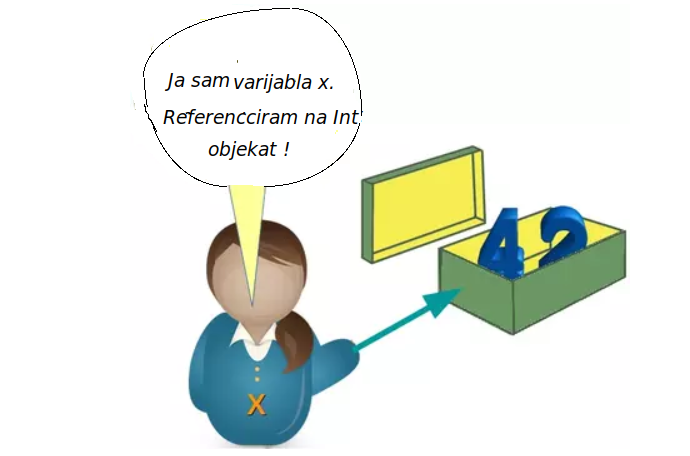
\includegraphics[width=140pt,height=100pt]{slike/variable_object.png}
 	\caption{Promjenljiva \texttt{x} referencira objekat vrijednosti 42.}
 	\label{fig:var_object}
 \end{figure}
 
 Ako zatim napišemo
 
 \begin{minted}{python}
 	y = x
 \end{minted}
 
 promjenljiva \texttt{y} neće dobiti kopiju broja 42, već će referencirati isti objekat kao i promjenljiva \texttt{x}. Situacija je prikazana na Slici~\ref{fig:two_refs}.
 
 \begin{figure}[H]
 	\centering
 	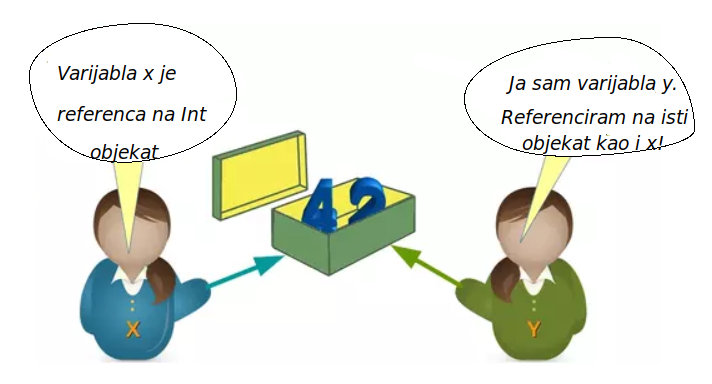
\includegraphics[width=140pt,height=100pt]{slike/point_two_vars.png}
 	\caption{Dvije promjenljive referenciraju isti objekat.}
 	\label{fig:two_refs}
 \end{figure}
 
 Ukoliko nakon toga izvršimo naredbu
 
 \begin{minted}{python}
 	y = 72
 \end{minted}
 
 promjenljiva \texttt{y} počinje referencirati novi objekat, dok \texttt{x} i dalje pokazuje na objekat koji predstavlja broj 42.
 
 \begin{figure}[H]
 	\centering
 	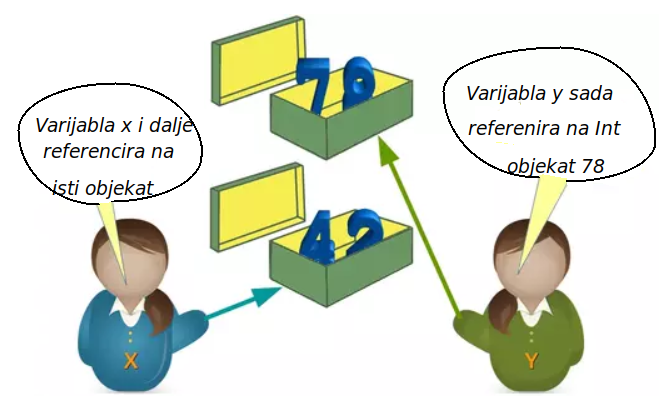
\includegraphics[width=140pt,height=100pt]{slike/vars_different_assigned.png}
 	\caption{Promjenljive referenciraju različite objekte.}
 \end{figure}
 
 Slično tome, promjenljivoj možemo dodijeliti objekat potpuno drugog tipa:
 
 \begin{minted}{python}
 	x = "Text"
 \end{minted}
 
 Nakon izvršavanja ove naredbe promjenljiva \texttt{x} više ne referencira objekat tipa \texttt{int}, već objekat tipa \texttt{str}.
 
 \begin{figure}[H]
 	\centering
 	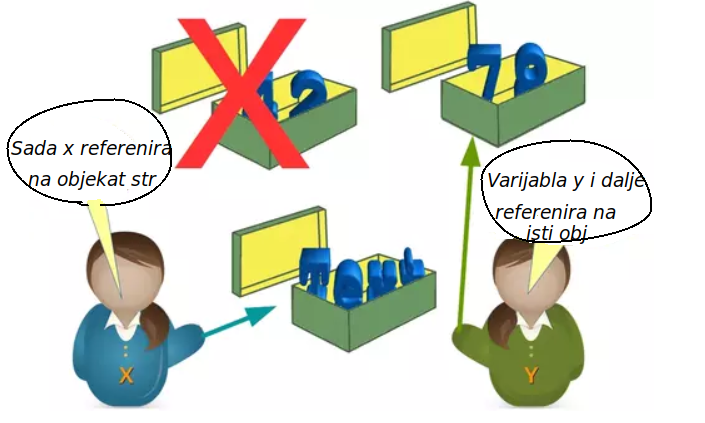
\includegraphics[width=140pt,height=100pt]{slike/varX_different_assigned.png}
 	\caption{Promjena reference promjenljive \texttt{x}.}
 \end{figure}
 
 Ovakvo ponašanje posljedica je činjenice da je Pajton dinamički tipiziran jezik. Tip se vezuje za objekat, a ne za promjenljivu. Zbog toga ista promjenljiva tokom izvršavanja programa može referencirati objekte različitih tipova.
 
 Ipak, od verzije Pajton 3.5 moguće je koristiti oznake tipova (\textit{type hints}) radi bolje čitljivosti programa:
 
 \begin{minted}{python}
 	x: str = "abc"
 	y: int = 23
 \end{minted}
 
 Napomenimo da ove oznake ne mijenjaju način rada jezika, već prvenstveno služe kao dokumentacija i pomoć alatima za statičku analizu koda.
 
 \subsection*{Upravljanje memorijom}
 
 Pajton automatski upravlja memorijom. Svaki objekat posjeduje brojač referenci koji prati koliko promjenljivih ili drugih objekata trenutno pokazuje na njega.
 
 Kada broj referenci nekog objekta postane jednak nuli, objekat više nije dostupan programu i njegova memorija može biti oslobođena. Pored toga, Pajton koristi i mehanizam sakupljanja otpadaka (\textit{garbage collection}) koji uklanja objekte koji više nisu potrebni, uključujući i složenije slučajeve kružnih referenci.
 
 Zahvaljujući ovim mehanizmima, programer uglavnom ne mora ručno voditi računa o dodjeljivanju i oslobađanju memorije, što značajno pojednostavljuje razvoj programa.
 
 Adresu objekta na koji referencira promjenljiva moguće je dobiti pomoću funkcije \texttt{id()}:
 
 \begin{minted}{python}
 	idnum = id(x)
 	idhex = hex(id(x))
 \end{minted}
 
 Dobijena vrijednost predstavlja jedinstveni identifikator objekta tokom njegovog životnog vijeka.
 
 \subsection*{Ispis i komentari}
 
 Ispis rezultata na ekran vrši se pomoću funkcije \texttt{print()}:
 
 \begin{minted}{python}
 	print("Pozdrav svijete!")
 	print(x)
 \end{minted}
 
 Funkcija \texttt{print()} može prikazati tekst, brojeve i druge objekte. Prije ispisa, objekat se po potrebi pretvara u tekstualni oblik.
 
 Komentari služe za dokumentovanje programa i ne izvršavaju se tokom rada programa.
 
 Jednolinijski komentar započinje znakom {\#}:
 
 \begin{minted}{python}
 	
 	# Ovo je komentar
 	
 	x = 5
 \end{minted}
 
 Za višelinijske komentare ili dokumentacione stringove najčešće se koriste trostruki navodnici:
 
 \begin{minted}{python}
 	"""
 	Ovo je višelinijski komentar
 	ili dokumentacioni string.
 	"""
 \end{minted}
 
 Komentari povećavaju čitljivost programa i olakšavaju njegovo održavanje, naročito kod većih projekata.
 

\section{Osnovni numerički tipovi podataka}

Numerički tipovi podataka koriste se za predstavljanje brojeva i izvođenje aritmetičkih operacija nad njima. Pajton podržava nekoliko numeričkih tipova, od kojih su najvažniji \texttt{int}, \texttt{float} i \texttt{complex}.

\subsection{Cjelobrojni i realni brojevi}

Tip \texttt{int} (skraćeno od \textit{integer}) koristi se za predstavljanje cijelih brojeva, dok tip \texttt{float} (skraćeno od \textit{floating-point number}) služi za predstavljanje realnih brojeva.

Primjeri inicijalizacije ovih tipova dati su u nastavku:

\begin{minted}{python}
	x = 5         # int
	y = -3        # int
	
	z = 3.14      # float
	w = -0.325    # float
\end{minted}

Nad numeričkim tipovima moguće je primjenjivati standardne aritmetičke operacije kao što su sabiranje (\texttt{+}), oduzimanje (\texttt{-}), množenje (\texttt{*}) i dijeljenje (\texttt{/}).

Posebnu pažnju treba obratiti na operatore dijeljenja:

\begin{itemize}
	\item \texttt{/} -- realno dijeljenje;
	\item \texttt{//} -- cjelobrojno dijeljenje.
\end{itemize}

Na primjer:

\begin{minted}{python}
	print(5 / 2)   # 2.5
	print(5 // 2)  # 2
\end{minted}

Pored osnovnih operatora, Pajton pruža i veliki broj ugrađenih funkcija za rad sa brojevima. Neke od najčešće korištenih su:

\begin{itemize}
	\item \texttt{abs(x)} -- apsolutna vrijednost broja;
	\item \texttt{round(x)} -- zaokruživanje broja;
	\item \texttt{min(...)} -- najmanja vrijednost;
	\item \texttt{max(...)} -- najveća vrijednost.
\end{itemize}

\begin{example}
	\begin{minted}{python}
		print(abs(-7))          # 7
		print(round(3.14159,2)) # 3.14
		print(min(2, 5, -1))    # -1
		print(max(2, 5, -1))    # 5
	\end{minted}
\end{example}

\subsection{Kompleksni brojevi}

Tip \texttt{complex} koristi se za predstavljanje kompleksnih brojeva oblika

$
a+bj,
$

gdje su $a$ i $b$ realni brojevi, dok simbol \texttt{j} predstavlja imaginarnu jedinicu.

Primjer rada sa kompleksnim brojevima:

\begin{minted}{python}
	x = 1 + 1j
	y = 2 + 1j
	
	z = x + y
	
	print(z)       # (3+2j)
	print(z.real)  # 3.0
	print(z.imag)  # 2.0
\end{minted}

Realni i imaginarni dio kompleksnog broja mogu se dobiti pomoću atributa \texttt{real} i \texttt{imag}.

Kompleksni broj moguće je kreirati i korišćenjem funkcije \texttt{complex()}:

\begin{minted}{python}
	z = complex(3, 2)
	print(z)   # (3+2j)
\end{minted}

Prvi argument predstavlja realni dio, dok drugi argument predstavlja imaginarni dio kompleksnog broja.

\section{Naredbe grananja i petlje}

U ovoj sekciji upoznaćemo osnovne kontrolne strukture programskog jezika Pajton: naredbu grananja \texttt{if} te petlje \texttt{for} i \texttt{while}.

Prije toga, u Tabeli~\ref{fig: operatori_poredjenja} dati su najčešće korišteni operatori poređenja.

Svaki izraz poređenja vraća logičku vrijednost \texttt{True} ili \texttt{False}, u zavisnosti od toga da li je odgovarajući uslov ispunjen.

\begin{table}[H]
	\caption{Osnovni operatori poređenja u Pajtonu.}
	\label{fig: operatori_poredjenja}
	
	\centering
	\scalebox{0.85}{
	\begin{tabular}{lll}
		\textbf{Matematička notacija} &
		\textbf{Pajtonova notacija} &
		\textbf{Značenje} \\ \hline
		
		$a < b$ & \texttt{a < b} &
		$a$ je manje od $b$ \\
		
		$a \leq b$ & \texttt{a <= b} &
		$a$ je manje ili jednako od $b$ \\
		
		$a > b$ & \texttt{a > b} &
		$a$ je veće od $b$ \\
		
		$a \geq b$ & \texttt{a >= b} &
		$a$ je veće ili jednako od $b$ \\
		
		$a = b$ & \texttt{a == b} &
		$a$ je jednako $b$ \\
		
		$a \neq b$ & \texttt{a != b} &
		$a$ nije jednako $b$ \\ \hline
	\end{tabular}}
	
\end{table}

\subsection{Uslovna naredba \texttt{if}}

Najjednostavniji oblik naredbe grananja dat je sljedećom sintaksom:

\begin{minted}{python}
	if uslov:
	    naredba_1
	else:
	    naredba_2
\end{minted}

Tok izvršavanja je jednostavan:

\begin{itemize}
	\item ako je uslov tačan, izvršava se blok \texttt{naredba\_1};
	\item u suprotnom se izvršava blok \texttt{naredba\_2}.
\end{itemize}

Posebno treba obratiti pažnju na uvlačenje koda (\textit{indentation}). Za razliku od mnogih drugih programskih jezika, u Pajtonu uvlačenje nije samo pitanje stila, već predstavlja dio sintakse jezika.

Nakon izvršavanja odgovarajućeg bloka program nastavlja sa prvom naredbom koja se nalazi izvan \texttt{if}-strukture.

U situacijama kada postoji više alternativa koristi se naredba \texttt{elif}:

\begin{minted}{python}
	if uslov_1:
	    naredba_1
	elif uslov_2:
	    naredba_2
	elif uslov_3:
	    naredba_3
	else:
	    naredba_n
\end{minted}

Uslovi se provjeravaju redom, od vrha prema dnu. Čim se pronađe prvi tačan uslov, izvršava se odgovarajući blok naredbi, nakon čega se ostatak strukture preskače.

Ako nijedan od uslova nije zadovoljen, izvršava se blok pod granom \texttt{else}.

\subsection{For i While petlje}

Petlje predstavljaju kontrolne strukture koje omogućavaju višestruko izvršavanje istog bloka koda. Koriste se kada je potrebno ponoviti određene operacije unaprijed poznat broj puta ili sve dok je zadovoljen određeni uslov.

Pajton podržava dvije osnovne vrste petlji:

\begin{itemize}
	\item \texttt{for} petlju;
	\item \texttt{while} petlju.
\end{itemize}

\subsubsection*{\texttt{for} petlja}

\texttt{for} petlja koristi se za prolazak kroz elemente iterabilnih objekata, kao što su liste, torke, stringovi, skupovi i rječnici.

Njena osnovna sintaksa je:

\begin{minted}{python}
	for item in iterable:
	    naredba
\end{minted}

Promjenljivoj \texttt{item} redom se dodjeljuju elementi kolekcije \texttt{iterable}, a za svaki element izvršava se odgovarajući blok koda.

Na primjer:

\begin{minted}{python}
	for broj in [1, 2, 3, 4]:
	    print(broj)
\end{minted}

Izvršavanjem ovog programa na ekran će biti ispisani brojevi 1, 2, 3 i 4.

Vrlo često se \texttt{for} petlja koristi zajedno sa funkcijom \texttt{range()}:

\begin{minted}{python}
	for i in range(5):
	    print(i)
\end{minted}

Ovaj kod ispisuje brojeve od 0 do 4.

\subsubsection*{\texttt{while} petlja}

\texttt{while} petlja izvršava blok koda sve dok je zadovoljen zadati logički uslov.

Njena osnovna sintaksa je:

\begin{minted}{python}
	while uslov:
	    naredba
\end{minted}

Prije svake iteracije provjerava se vrijednost izraza \texttt{uslov}. Ako je njegova vrijednost \texttt{True}, izvršava se tijelo petlje. Kada uslov postane netačan (\texttt{False}), izvršavanje petlje se završava, a program nastavlja sa prvom naredbom nakon petlje.

Na primjer, prvih deset parnih prirodnih brojeva može se ispisati na sljedeći način:

\begin{minted}{python}
	i = 1
	
	while i <= 10:
	    print(2 * i)
	    i += 1
\end{minted}

Naredba
\begin{minted}{python}
	i += 1
\end{minted}
predstavlja skraćeni zapis za

\begin{minted}{python}
	i = i + 1
\end{minted}

i koristi se za povećavanje vrijednosti promjenljive za jedan.

\section{Složene strukture podataka}

Pored osnovnih numeričkih tipova podataka, Pajton pruža i niz složenijih struktura podataka koje omogućavaju efikasno organizovanje i obradu većih količina informacija.

Najvažnije među njima su:

\begin{itemize}
	\item stringovi (\texttt{str});
	\item liste (\texttt{list});
	\item torke (\texttt{tuple});
	\item skupovi (\texttt{set});
	\item rječnici (\texttt{dict}).
\end{itemize}

Sve navedene strukture predstavljaju kolekcije objekata i koriste se u gotovo svakom ozbiljnijem programu.

\subsection{Stringovni tip podataka}

Tip \texttt{str} predstavlja ugrađeni tip podataka namijenjen radu sa tekstom. String se može posmatrati kao uređena sekvenca Unicode znakova.

Jedna od najvažnijih osobina stringova jeste da su \textit{nepromjenjivi} (\textit{immutable}). Nakon što se string kreira, njegov sadržaj nije moguće direktno mijenjati. Svaka izmjena zapravo rezultuje kreiranjem novog string objekta.

\subsubsection*{Inicijalizacija stringova}

String se može definisati korišćenjem jednostrukih ili dvostrukih navodnika:

\begin{minted}{python}
	string0 = 'hello'
	string1 = "world"
\end{minted}

Za višelinijske stringove koriste se trostruki navodnici:

\begin{minted}{python}
	multiline_str = """
	Ovo je
	višelinijski string.
	"""
\end{minted}

\subsubsection*{Osnovne operacije nad stringovima}

\begin{itemize}
	
	\item \textbf{Konkatenacija}
	
	Stringovi se mogu spajati pomoću operatora \texttt{+}:
	
	\begin{minted}{python}
		ime = "Marko"
		prezime = "Markovic"
		
		print(ime + " " + prezime)
	\end{minted}
	

	\item \textbf{Pristup pojedinačnim znakovima}
	
	Znakovima stringa pristupa se pomoću operatora indeksiranja \texttt{[]}.
	```
	
	\begin{minted}{python}
		tekst = "Python"
		
		print(tekst[0])   # P
		print(tekst[-1])  # n
	\end{minted}
	
	Pozitivni indeksi broje se od početka stringa, dok negativni indeksi broje od kraja stringa.
	
	\item \textbf{Rezanje stringa (slicing)}
	
	Dio stringa može se izdvojiti pomoću operatora \texttt{[:]}:
	
	\begin{minted}{python}
		tekst = "world"
		
		print(tekst[1:3])  # or
		print(tekst[:3])   # wor
		print(tekst[2:])   # rld
	\end{minted}
	
	\item \textbf{Ponavljanje stringa}
	
	Operator \texttt{*} omogućava višestruko ponavljanje stringa:
	
	\begin{minted}{python}
		print("abc" * 3)
	\end{minted}
	
	Rezultat je:
	
	\begin{minted}{text}
		abcabcabc
	\end{minted}
	\item \textbf{Dužina stringa}
	
	Broj znakova u stringu dobija se funkcijom \texttt{len()}:
	
	\begin{minted}{python}
		print(len("Python"))
	\end{minted}
	
	\item \textbf{Brisanje reference}
	
	Ključna riječ \texttt{del} uklanja referencu na objekat:
	
	\begin{minted}{python}
		tekst = "abc"
		del tekst
	\end{minted}
	
\end{itemize}

\subsubsection*{Korisne metode}

Klasa \texttt{str} sadrži veliki broj ugrađenih metoda. Neke od najčešće korištenih su:

\begin{itemize}
	\item \texttt{lower()} -- pretvara sva slova u mala;
	\item \texttt{upper()} -- pretvara sva slova u velika;
	\item \texttt{strip()} -- uklanja praznine sa početka i kraja stringa;
	\item \texttt{replace()} -- zamjenjuje dio stringa drugim tekstom;
	\item \texttt{find()} -- pronalazi poziciju podstringa.
\end{itemize}

Njihovu detaljniju upotrebu prikazaćemo kroz naredne primjere.

\textit{Memorijska organizacija}. Stringovi se u Pajtonu predstavljaju kao uređene sekvence Unicode znakova smještene u neprekidnom dijelu memorije. Svakom znaku pridružen je odgovarajući Unicode k\^od, što omogućava rad sa tekstom na velikom broju svjetskih jezika.

Pojednostavljen prikaz memorijske organizacije stringa

\begin{minted}{python}
	x = "code"
\end{minted}

dat je na Slici~\ref{fig:str_mem}.

\begin{figure}[H]
	\centering
	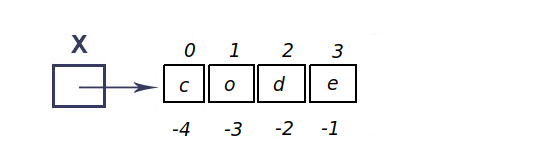
\includegraphics[width=200pt,height=60pt]{slike/str_mem_organization.png}
	\caption{Pojednostavljen prikaz memorijske organizacije stringa \texttt{"code"}.}
	\label{fig:str_mem}
\end{figure}

Za razliku od nekih drugih programskih jezika, stringovi u Pajtonu su \textit{nepromjenjivi} (\textit{immutable}). To znači da se sadržaj postojećeg stringa ne može direktno mijenjati. Svaka operacija koja naizgled mijenja string zapravo kreira novi string objekat.

Na primjer:

\begin{minted}{python}
	s = "code"
	s = s + "!"
\end{minted}

Nakon izvršavanja druge naredbe kreira se novi string \texttt{"code!"}, dok originalni string ostaje nepromijenjen.

\textit{Dodatna napomena}. Pajton interno koristi različite optimizacije za rad sa stringovima. Jedna od njih je \textit{interniranje stringova} (\textit{string interning}), pri čemu se identični stringovi po potrebi mogu dijeliti između više promjenljivih. Time se smanjuje potrošnja memorije i poboljšavaju performanse programa.

\subsubsection*{Formatiranje stringova}

Prilikom ispisa rezultata često je potrebno kombinovati tekst i vrijednosti promjenljivih. Pajton nudi nekoliko načina za formatiranje stringova.

Jedan od tradicionalnih pristupa koristi metodu \texttt{format()}:

\begin{minted}{python}
	print("Moje ime je {0}, a prezime {1}".
	       format("Marko", "Marković"))
\end{minted}

Vrijednost označena sa \texttt{{0}} zamjenjuje se prvim argumentom funkcije \texttt{format()}, dok se \texttt{{1}} zamjenjuje drugim argumentom.

Savremeniji i danas preporučeni način predstavljaju formatirani stringovi (\textit{f-strings}):

\begin{minted}{python}
	ime = "Marko"
	godine = 32
	print(f"Ime: {ime}, godine: {godine}")
\end{minted}

Kod f-stringova vrijednosti promjenljivih navode se direktno unutar vitičastih zagrada, što k\^od čini preglednijim i jednostavnijim za pisanje.

Zbog svoje čitljivosti i efikasnosti, f-stringovi predstavljaju preporučeni način formatiranja stringova u savremenom Pajtonu.


\subsection{Liste}

Lista predstavlja uređenu, indeksiranu i promjenljivu kolekciju elemenata. U Pajtonu se implementira pomoću ugrađenog tipa podataka \texttt{list}.

Za razliku od mnogih drugih programskih jezika, elementi liste ne moraju biti istog tipa. Zbog toga kažemo da su liste \textit{heterogene} kolekcije. Na primjer, ista lista može sadržavati brojeve, stringove, logičke vrijednosti i druge objekte.

Elementi liste indeksiraju se brojevima počevši od nule. Pored standardnog indeksiranja, Pajton podržava i negativne indekse. Pri tome indeks \texttt{-1} označava posljednji element liste, \texttt{-2} pretposljednji itd.

\subsubsection*{Inicijalizacija lista}

Liste se mogu kreirati na više načina:

\begin{minted}{python}
	lista = list()
	lista1 = ["a", "b", 2.0, 3]	
	lista2 = list(("abc", "def", 2))
\end{minted}

\subsubsection*{Pristup elementima}

Pojedinačnim elementima liste pristupa se pomoću operatora \texttt{[]}.

\begin{minted}{python}
	lista = [10, 20, 30]
	print(lista[0])   # 10
	print(lista[-1])  # 30
\end{minted}

U prvom slučaju pristupa se prvom elementu liste, dok se u drugom slučaju koristi negativni indeks za pristup posljednjem elementu.

\subsubsection*{Rezanje liste (slicing)}

Dio liste može se izdvojiti pomoću operatora

\begin{minted}{python}
	lista[indeks1:indeks2:korak]
\end{minted}

pri čemu se uzimaju elementi od pozicije \texttt{indeks1} do pozicije \texttt{indeks2} (isključivo), uz zadani korak.

\begin{minted}{python}
	lista = [0, 1, 2, 3, 4, 5]
	print(lista[1:4])   # [1, 2, 3]
	print(lista[:3])    # [0, 1, 2]
	print(lista[::2])   # [0, 2, 4]
\end{minted}

Rezultat operacije rezanja uvijek je nova lista.

\subsubsection*{Provjera pripadnosti}

Operator \texttt{in} koristi se za provjeru da li se određeni element nalazi u listi.

\begin{minted}{python}
	if 5 in lista:
	    print("Pronađen element")
\end{minted}

Vrijednost izraza je \texttt{True} ako se element nalazi u listi, odnosno \texttt{False} u suprotnom.

\subsubsection*{Iteriranje kroz listu}

Elementima liste može se pristupati jedan po jedan pomoću \texttt{for} petlje.

\begin{minted}{python}
	for x in lista:
	    print(x)
\end{minted}

Ovakav način prolaska kroz listu predstavlja jednu od najčešće korištenih programskih konstrukcija u Pajtonu.

\subsubsection*{Dodavanje i brisanje elemenata}

Novi element može se dodati na kraj liste metodom \texttt{append()}:

\begin{minted}{python}
	lista.append(10)
\end{minted}

Element se uklanja metodom \texttt{remove()}, pri čemu se briše prvo pojavljivanje zadate vrijednosti:

\begin{minted}{python}
	lista.remove(10)
\end{minted}

Posljednji element liste može se ukloniti metodom \texttt{pop()}:

\begin{minted}{python}
	lista.pop()
\end{minted}

Metoda \texttt{pop()} vraća uklonjeni element, što je često korisno u praksi.

\subsubsection*{Umetanje elemenata}

Element se može umetnuti na proizvoljnu poziciju korištenjem metode \texttt{insert()}:

\begin{minted}{python}
	lista.insert(2, 100)
\end{minted}

Nakon izvršavanja ove naredbe vrijednost \texttt{100} nalaziće se na poziciji 2, dok će svi naredni elementi biti pomjereni za jedno mjesto udesno.

\subsubsection*{Obrtanje i kopiranje liste}

Redoslijed elemenata liste može se obrnuti metodom \texttt{reverse()}:

\begin{minted}{python}
	lista.reverse()
\end{minted}

Kopija liste kreira se metodom \texttt{copy()}:

\begin{minted}{python}
	nova_lista = lista.copy()
\end{minted}

Na ovaj način dobija se nova lista koja sadrži iste elemente kao i originalna lista.

\subsubsection*{Najčešće korištene metode}

Tabela~\ref{tab:list_methods} daje pregled najvažnijih metoda klase \texttt{list}.

\begin{table}[H]
	\centering
	\caption{Najčešće korištene metode liste.}
	\label{tab:list_methods}
	\begin{tabular}{l|l}
		\hline
		\textbf{Metoda} & \textbf{Opis} \\ \hline
		\texttt{append(x)} & Dodaje element na kraj liste \\
		\texttt{insert(i,x)} & Umeće element na poziciju \texttt{i} \\
		\texttt{remove(x)} & Briše prvo pojavljivanje elementa \\
		\texttt{pop()} & Uklanja i vraća posljednji element \\
		\texttt{reverse()} & Obrće redoslijed elemenata \\
		\texttt{copy()} & Kreira kopiju liste \\
		\texttt{clear()} & Briše sve elemente liste \\
		\texttt{sort()} & Sortira elemente liste \\
		\hline
	\end{tabular}
\end{table}

\subsubsection*{Memorijska organizacija}

Liste su u Pajtonu implementirane kao \textit{dinamički nizovi} (eng. \textit{dynamic arrays}). To znači da se njihova veličina može mijenjati tokom izvršavanja programa, za razliku od klasičnih nizova čija je veličina unaprijed fiksirana.

Prilikom kreiranja liste interpreter rezerviše određeni memorijski prostor za smještanje elemenata. Kada se lista proširi i raspoloživi kapacitet više nije dovoljan za pohranu novih elemenata, automatski se dodjeljuje veći memorijski blok, nakon čega se postojeći elementi kopiraju u novu memorijsku oblast. Ovaj postupak naziva se \textit{realokacija memorije}.

Kako bi se smanjio broj realokacija, Pajton obično rezerviše nešto više memorije nego što je trenutno potrebno. Zahvaljujući tome, dodavanje novih elemenata na kraj liste najčešće se izvršava veoma efikasno.

Pojednostavljen prikaz memorijske organizacije liste i torke dat je na Slici~\ref{fig:mem_list_org}.

\begin{figure}[H]
	\centering
	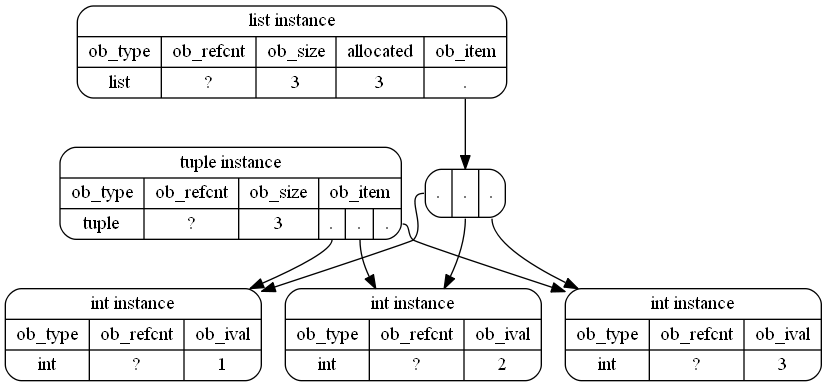
\includegraphics[width=300pt,height=160pt]{slike/img-list-tuple.png}
	\caption{Pojednostavljen prikaz memorijske organizacije liste i torke.}
	\label{fig:mem_list_org}
\end{figure}

U situacijama kada je unaprijed poznat maksimalan broj elemenata koji će se koristiti, često se kreira lista željene veličine:

\begin{minted}{python}
	lista = [None] * max_broj_elemenata
\end{minted}

Na ovaj način izbjegava se veliki broj naknadnih proširenja liste, što može pozitivno uticati na performanse programa.

\subsubsection*{Dodatne napomene}

Za razliku od klasičnih nizova u programskom jeziku \texttt{C}, liste u Pajtonu mogu sadržavati elemente različitih tipova:

\begin{minted}{python}
	lista = [1, "tekst", 3.14, True]
\end{minted}

Ova osobina čini liste veoma fleksibilnim i jednostavnim za upotrebu. Međutim, takva fleksibilnost ima svoju cijenu. Svaki element liste predstavlja zaseban Pajtonov objekat, koji pored stvarne vrijednosti sadrži i dodatne informacije, kao što su tip objekta i broj referenci na njega.

Interno posmatrano, lista ne sadrži same objekte već niz pokazivača na odgovarajuće objekte u memoriji. Zbog toga liste zauzimaju više memorijskog prostora nego homogeni nizovi implementirani u jezicima nižeg nivoa.

U većini praktičnih primjena liste predstavljaju osnovnu i najčešće korištenu strukturu podataka u Pajtonu. Zahvaljujući jednostavnoj sintaksi, podršci za dinamičko proširivanje i velikom broju ugrađenih metoda, one su često prvi izbor za organizaciju i obradu kolekcija podataka.

\subsection{Nizovi: modul \texttt{array}}

Pored lista, Pajton nudi i modul \texttt{array}, koji omogućava rad sa homogenim nizovima podataka. Po svojoj organizaciji i načinu korištenja, objekti tipa \texttt{array} slični su nizovima u programskim jezicima \textit{C} i \textit{C++}.

Za razliku od lista, koje mogu sadržavati elemente različitih tipova, svi elementi objekta \texttt{array} moraju biti istog tipa. Zbog toga se podaci mogu skladištiti efikasnije i zauzimati manje memorijskog prostora.

Elementi niza smješteni su u neprekidnom bloku memorije, što omogućava brz pristup proizvoljnom elementu korištenjem njegovog indeksa. Indeksiranje elemenata počinje od nule, kao i kod lista.

Prilikom kreiranja objekta tipa \texttt{array} potrebno je navesti oznaku tipa podataka (\textit{typecode}) koji će se skladištiti. Najčešće korištene oznake prikazane su u Tabeli~\ref{tab:TipPodatakaArray}.

\begin{table}[H]
	\caption{Najčešće korišteni tipovi podataka u modulu \texttt{array}.}
	\label{tab:TipPodatakaArray}
	\centering
	\begin{tabular}{llll}
		\hline
		\textbf{Typecode} & \textbf{Tip podatka} & \textbf{Pajtonov tip} & \textbf{Veličina (B)} \\
		\hline
		\texttt{'b'} / \texttt{'B'} & signed / unsigned char & int & 1 \\
		\texttt{'h'} / \texttt{'H'} & signed / unsigned short & int & 2 \\
		\texttt{'i'} / \texttt{'I'} & signed / unsigned int & int & 4 \\
		\texttt{'l'} / \texttt{'L'} & signed / unsigned long & int & 4 \\
		\texttt{'q'} / \texttt{'Q'} & signed / unsigned long long & int & 8 \\
		\texttt{'f'} & float & float & 4 \\
		\texttt{'d'} & double & float & 8 \\
		\hline
	\end{tabular}
\end{table}

Da bismo koristili modul \texttt{array}, potrebno ga je prethodno uključiti:

\begin{minted}{python}
	import array
\end{minted}

\subsubsection*{Inicijalizacija}

Objekat tipa \texttt{array} kreira se navođenjem oznake tipa i početnih vrijednosti:

\begin{minted}{python}
	from array import array
	
	my_array = array('i', [1, 2, 3, 4, 5])
\end{minted}

U ovom primjeru oznaka \texttt{'i'} označava cjelobrojne vrijednosti tipa \texttt{int}.

\subsubsection*{Osnovne operacije}

\begin{itemize}
	
	\item \textbf{Pristup elementima}
	
	\begin{minted}{python}
		print(my_array[0])   # 1
		print(my_array[2])   # 3
	\end{minted}
	
	\item \textbf{Izmjena elemenata}
	
	\begin{minted}{python}
		my_array[0] = 7
		print(my_array)
		# array('i', [7, 2, 3, 4, 5])
		
	\end{minted}
	
	\item \textbf{Dodavanje elementa na kraj niza}
	
	\begin{minted}{python}
		my_array.append(10)
	\end{minted}
	
	\item \textbf{Dodavanje više elemenata}
	
	\begin{minted}{python}
		from array import array
		
		floats = array('f', [2.0, 3.2, 1.4])
		floats.extend([1.1, 4.1, 5.2, 9.0])
	\end{minted}
	
	\item \textbf{Umetanje elementa}
	
	\begin{minted}{python}
		my_array.insert(2, 100)
	\end{minted}
	
	\item \textbf{Brisanje elementa}
	
	\begin{minted}{python}
		my_array.remove(100)
	\end{minted}
	
	\item \textbf{Uklanjanje posljednjeg elementa}
	
	\begin{minted}{python}
		my_array.pop()
	\end{minted}
	
\end{itemize}

\subsubsection*{Kada koristiti \texttt{array}?}

Modul \texttt{array} je posebno koristan kada radimo sa velikim kolekcijama numeričkih podataka istog tipa. U poređenju sa listama, objekti tipa \texttt{array} zauzimaju manje memorije i omogućavaju efikasnije skladištenje homogenih podataka.

Ipak, u naučnom računarstvu i analizi podataka danas se mnogo češće koriste strukture iz biblioteke \texttt{NumPy}, koje predstavljaju proširenje ideje homogenih nizova i nude znatno veće performanse i bogatiji skup funkcionalnosti.




\subsection{Rječnici}

Rječnik (\texttt{dict}) predstavlja jednu od najvažnijih ugrađenih struktura podataka u Pajtonu. Riječ je o promjenljivoj kolekciji elemenata organizovanih u obliku parova \emph{ključ--vrijednost}.

Za razliku od lista, gdje se elementima pristupa pomoću numeričkih indeksa, u rječnicima se pristup vrši preko ključeva. Svakom ključu pridružena je tačno jedna vrijednost, pri čemu ključevi moraju biti jedinstveni unutar rječnika.

Rječnici se često nazivaju i \textit{heš mapama} (eng. \textit{hash maps}), jer su interno implementirani korištenjem heš tabela.

\subsubsection*{Inicijalizacija}

Rječnik se može kreirati na više načina.

\begin{minted}{python}
	
	# Kreiranje pomoću vitičastih zagrada
	
	dct = {
		"ime": "Mirko",
		"godine": 30,
		"grad": "Banja Luka"
	}
	
	# Kreiranje pomoću konstruktora dict()
	
	dct1 = dict(
	ime="Mirko",
	godine=30,
	grad="Banja Luka"
	)
\end{minted}

\subsubsection*{Osnovne operacije}

\begin{itemize}
	
	\item \textbf{Pristup vrijednosti}
	
	Vrijednost pridružena određenom ključu dobija se korištenjem operatora \texttt{[]}.
	
	\begin{minted}{python}
		dct = {
			"ime": "Mirko",
			"godine": 30,
			"grad": "Banja Luka"
		}
		
		print(dct["ime"])      # Mirko
	\end{minted}
	
	\item \textbf{Dodavanje i izmjena elemenata}
	
	\begin{minted}{python}
		dct["godine"] = 31
	\end{minted}
	
	Ako ključ već postoji, njegova vrijednost se ažurira. U suprotnom se dodaje novi par ključ--vrijednost.
	
	\item \textbf{Brisanje elementa}
	
	Element se može ukloniti korištenjem ključne riječi \texttt{del} ili metode \texttt{pop()}.
	
	\begin{minted}{python}
		del dct["grad"]
	\end{minted}
	
	ili
	
	\begin{minted}{python}
		dct.pop("grad")
	\end{minted}
	
	\item \textbf{Provjera postojanja ključa}
	
	Operator \texttt{in} provjerava da li se određeni ključ nalazi u rječniku.
	
	\begin{minted}{python}
		print("ime" in dct)      # True
		print("pol" in dct)      # False
	\end{minted}
	
	\item \textbf{Iteriranje kroz rječnik}
	
	\begin{minted}{python}
		for kljuc, vrijednost in dct.items():
		print(kljuc, vrijednost)
	\end{minted}
	
	\item \textbf{Korisne metode}
	
	\begin{itemize}
		\item \texttt{len(dct)} -- vraća broj elemenata rječnika;
		\item \texttt{keys()} -- vraća kolekciju svih ključeva;
		\item \texttt{values()} -- vraća kolekciju svih vrijednosti;
		\item \texttt{items()} -- vraća parove (ključ, vrijednost);
		\item \texttt{get(kljuc)} -- sigurno dohvaća vrijednost bez generisanja greške ukoliko ključ ne postoji.
	\end{itemize}
	
\end{itemize}

\subsubsection*{Memorijska organizacija}

Rječnici su u Pajtonu implementirani korištenjem heš tabela. Osnovna ideja sastoji se u tome da se svaki ključ transformiše u cijeli broj primjenom heš funkcije. Dobijena vrijednost koristi se za brzo pronalaženje mjesta na kojem se nalazi odgovarajuća vrijednost.

Zahvaljujući ovakvoj organizaciji, osnovne operacije nad rječnicima imaju očekivanu vremensku složenost:

\begin{itemize}
	\item pristup elementu: $O(1)$,
	\item dodavanje elementa: $O(1)$,
	\item brisanje elementa: $O(1)$.
\end{itemize}

U najgorem slučaju ove operacije mogu biti sporije zbog pojave kolizija, ali se u praksi takve situacije rijetko javljaju.

Prilikom kreiranja rječnika interpreter rezerviše određeni broj mjesta u heš tabeli. Kako broj elemenata raste, tabela se po potrebi automatski proširuje kako bi se očuvala efikasnost pristupa.

Pojednostavljen prikaz organizacije rječnika dat je na Slici~\ref{fig:dict_mem_organization}.

\begin{figure}[H]
	\centering
	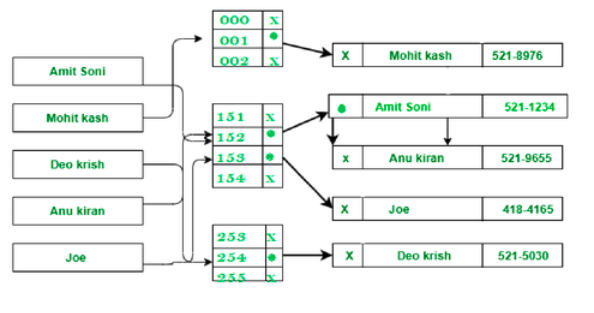
\includegraphics[width=300pt,height=160pt]{slike/dict_mem_organization.png}
	\caption{Pojednostavljen prikaz unutrašnje organizacije rječnika u Pajtonu.}
	\label{fig:dict_mem_organization}
\end{figure}

\subsubsection*{Dodatne napomene}

Ključevi u rječniku moraju biti nepromjenljivi objekti. Zbog toga se kao ključevi mogu koristiti objekti tipa \texttt{int}, \texttt{float}, \texttt{str} ili \texttt{tuple}, dok liste (\texttt{list}) ne mogu biti ključevi.

\begin{minted}{python}
	dct = {
		"ime": "Mirko",
		123: "identifikator",
		(1, 2): "par brojeva"
	}
\end{minted}

Zbog veoma brzog pristupa podacima, rječnici predstavljaju jednu od najčešće korištenih struktura podataka u modernom programiranju. Posebno su korisni kada je potrebno efikasno pretraživanje, grupisanje ili indeksiranje podataka.



\subsection{Skupovi}

Skup (\texttt{set}) predstavlja neuređenu kolekciju jedinstvenih elemenata. Po svojim osobinama odgovara matematičkom pojmu skupa: redoslijed elemenata nije važan, a duplikati nisu dozvoljeni.

Osnovna namjena skupova jeste efikasna provjera pripadnosti elementa kolekciji. Zbog toga se često koriste u algoritmima koji zahtijevaju brzo pretraživanje ili eliminisanje duplikata.

Elementi skupa mogu biti objekti nepromjenljivih tipova podataka, kao što su \texttt{int}, \texttt{float}, \texttt{str}, \texttt{tuple} ili \texttt{complex}. Sa druge strane, promjenljive kolekcije poput lista (\texttt{list}), rječnika (\texttt{dict}) i drugih skupova (\texttt{set}) ne mogu biti elementi skupa.

\subsubsection*{Inicijalizacija}

Skup se može kreirati na nekoliko načina:

\begin{minted}{python}
	skup = set()
	
	skup1 = {1, 2, 3, 4}
	
	skup2 = set((1, 2, "3"))
	
	skup3 = set([1, 2, 3])
\end{minted}

\textbf{Napomena.} Prazan skup se kreira pomoću funkcije \texttt{set()}. Izraz

\begin{minted}{python}
	skup = {}
\end{minted}

ne kreira prazan skup već prazan rječnik.

\subsubsection*{Osnovne metode}

\begin{itemize}
	
	\item \texttt{add(elem)} -- dodaje element u skup;
	
	\begin{minted}{python}
		skup.add(5)
	\end{minted}
	
	\item \texttt{remove(elem)} -- uklanja element iz skupa; generiše grešku ukoliko element ne postoji;
	
	\begin{minted}{python}
		skup.remove(5)
	\end{minted}
	
	\item \texttt{discard(elem)} -- uklanja element ako postoji, bez generisanja greške;
	
	\begin{minted}{python}
		skup.discard(5)
	\end{minted}
	
	\item \texttt{pop()} -- uklanja i vraća proizvoljan element skupa;
	
	\item \texttt{clear()} -- uklanja sve elemente iz skupa;
	
	\item \texttt{union()} ili operator \texttt{|} -- vraća uniju dva skupa;
	
	\begin{minted}{python}
		A = {1, 2, 3}
		B = {3, 4, 5}
		
		print(A | B)
		
		# {1, 2, 3, 4, 5}
		
	\end{minted}
	
	\item \texttt{intersection()} ili operator \texttt{\&} -- vraća presjek dva skupa;
	
	\begin{minted}{python}
		print(A & B)
		
		# {3}
		
	\end{minted}
	
	\item \texttt{difference()} ili operator \texttt{-} -- vraća razliku skupova;
	
	\begin{minted}{python}
		print(A - B)
		
		# {1, 2}
		
	\end{minted}
	
	\item Operator \texttt{in} koristi se za provjeru pripadnosti elementa skupu;
	
	\begin{minted}{python}
		print(3 in A)   # True
		print(7 in A)   # False
	\end{minted}
	
\end{itemize}

\subsubsection*{Memorijska organizacija}

Skupovi su u Pajtonu implementirani korištenjem heš tabela. Svakom elementu pridružuje se heš vrijednost koja omogućava veoma brzo pronalaženje njegove pozicije u memoriji.

Zahvaljujući takvoj organizaciji, osnovne operacije nad skupovima imaju očekivanu vremensku složenost:

\begin{itemize}
	\item dodavanje elementa: $O(1)$;
	\item uklanjanje elementa: $O(1)$;
	\item provjera pripadnosti: $O(1)$.
\end{itemize}

U najgorem slučaju, zbog pojave većeg broja kolizija, složenost može porasti na $O(n)$, ali se takve situacije u praksi rijetko javljaju.

Sljedeći primjer pokazuje da je skup predstavljen ugrađenim tipom podataka \texttt{set}:

\begin{minted}{python}
	s = {1, 2, 3}
	
	print(type(s))
	
	# <class 'set'>
	
\end{minted}

Pojednostavljen prikaz organizacije skupa dat je na Slici~\ref{fig:set_mem_organization}.

\begin{figure}[H]
	\centering
	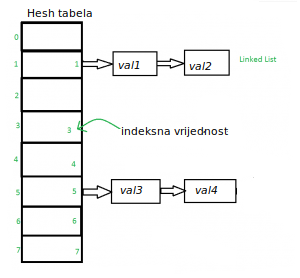
\includegraphics[width=220pt,height=150pt]{slike/set_mem_organization.png}
	\caption{Pojednostavljen prikaz unutrašnje organizacije skupa u Pajtonu.}
	\label{fig:set_mem_organization}
\end{figure}

\subsubsection*{Dodatne napomene}

Skupovi su naročito korisni kada je potrebno:

\begin{itemize}
	\item ukloniti duplikate iz kolekcije podataka;
	\item efikasno provjeriti da li se element nalazi u kolekciji;
	\item izvršavati skupovne operacije poput unije, presjeka i razlike.
\end{itemize}

Zbog veoma brzih operacija pretraživanja, skupovi predstavljaju jednu od najvažnijih struktura podataka u algoritmici i često se koriste za optimizaciju vremena izvršavanja programa.

\subsection{Torke}

Torka (\texttt{tuple}) predstavlja uređenu, indeksiranu i nepromjenljivu (\textit{immutable}) kolekciju elemenata. U Pajtonu se implementira pomoću ugrađenog tipa podataka \texttt{tuple}.

Za razliku od lista, elementi torke se ne mogu mijenjati nakon kreiranja objekta. Torke mogu sadržavati elemente različitih tipova podataka i dopuštaju pojavljivanje duplikata.

\subsubsection*{Inicijalizacija}

Torka se može kreirati na nekoliko načina:

\begin{minted}{python}
	my_tuple = ("aa", "bb", 2.0, 3)
	
	my_tuple1 = tuple(["abc", 3.2, "a"])
\end{minted}

Torka sa jednim elementom zahtijeva završni zarez:

\begin{minted}{python}
	t = (5,)
\end{minted}

Bez zareza izraz \texttt{(5)} predstavlja običan cjelobrojni objekat.

\subsubsection*{Osnovne operacije}

\begin{itemize}
	
	\item \textbf{Pristup elementima}
	
	Elementima torke pristupa se pomoću operatora \texttt{[]}:
	
	\begin{minted}{python}
		my_tuple = (1, 2, 3, 2, 4, 2, 5)
		
		print(my_tuple[2])   # 3
		print(my_tuple[-1])  # 5
	\end{minted}
	
	\item \textbf{Brojanje pojavljivanja elementa}
	
	Metoda \texttt{count()} vraća broj pojavljivanja elementa:
	
	\begin{minted}{python}
		my_tuple = (1, 2, 3, 2, 3, 5)
		
		print(my_tuple.count(2))  # 2
	\end{minted}
	
	\item \textbf{Pronalaženje indeksa elementa}
	
	Metoda \texttt{index()} vraća indeks prvog pojavljivanja elementa:
	
	\begin{minted}{python}
		print(my_tuple.index(2))  # 1
	\end{minted}
	
	\item \textbf{Dužina torke}
	
	Broj elemenata određuje se funkcijom \texttt{len()}:
	
	\begin{minted}{python}
		print(len(my_tuple))  # 6
	\end{minted}
	
	\item \textbf{Spajanje torki}
	
	Dvije torke mogu se spojiti operatorom \texttt{+}:
	
	\begin{minted}{python}
		t1 = ("a", "bb", 2)
		t2 = ("ee", 2, 3.4)
		t3 = t1 + t2
		print(t3)
		# ("a", "bb", 2, "ee", 2, 3.4)
		
	\end{minted}
	
	\item \textbf{Rezanje torke (slicing)}
	
	Kao i kod lista, moguće je izdvojiti dio torke:
	
	\begin{minted}{python}
		t = (0, 1, 2, 3, 4, 5)
		
		print(t[1:4])  # (1, 2, 3)
	\end{minted}
	
\end{itemize}

\subsubsection*{Memorijska organizacija}

Torke su nepromjenljive strukture podataka. Nakon kreiranja nije moguće dodavati, uklanjati niti mijenjati njihove elemente. Zbog toga Pajton može efikasnije upravljati memorijom nego kod promjenljivih struktura kao što su liste.

Objekat tipa \texttt{tuple} sadrži reference na svoje elemente. Pošto se broj elemenata ne može mijenjati nakon kreiranja torke, nije potrebno vršiti realokaciju memorije tokom izvršavanja programa.

Pristup elementima torke ostvaruje se direktnim indeksiranjem, pa je vremenska složenost operacije pristupa elementu jednaka $O(1)$.

Zbog svoje nepromjenljivosti, torke često zauzimaju manje memorije od lista sa istim brojem elemenata i mogu se koristiti kao ključevi u rječnicima ili kao elementi skupova, pod uslovom da svi njihovi elementi takođe budu nepromjenljivi.

Poređenje memorijske organizacije lista i torki prikazano je na Slici~\ref{fig:mem_list_org}.

\subsubsection*{Kada koristiti torke?}

Torke su pogodan izbor kada:

\begin{itemize}
	\item podaci ne treba da se mijenjaju nakon kreiranja;
	\item želimo smanjiti potrošnju memorije;
	\item želimo koristiti kolekciju kao ključ u rječniku ili element skupa;
	\item želimo jasno naglasiti da određeni skup podataka predstavlja jednu logičku cjelinu.
\end{itemize}

Tipični primjeri upotrebe su predstavljanje koordinata tačke, datuma, RGB boja i drugih nepromjenljivih zapisa podataka.

\section{Funkcije}

Funkcije predstavljaju jedan od osnovnih mehanizama za organizaciju programa. Njihova uloga je da složen problem podijele na manje, logički zaokružene cjeline koje se mogu višestruko koristiti.

U Pajtonu je svaka funkcija objekat. To znači da se funkcija može dodijeliti varijabli, proslijediti kao argument drugoj funkciji ili vratiti kao rezultat izvršavanja funkcije. Kada interpreter obradi definiciju funkcije, kreira se objekat tipa \texttt{function} koji sadrži informacije o nazivu funkcije, parametrima, tijelu funkcije i drugim metapodacima.

Funkcija se definiše pomoću ključne riječi \texttt{def}. Nakon naziva funkcije navode se parametri u zagradama, a tijelo funkcije se piše u uvučenom bloku koda. Naredba \texttt{return} služi za vraćanje rezultata i završetak izvršavanja funkcije.

\begin{minted}{python}
	def proizvod_brojeva(x, y):
	proizvod = x * y
	return proizvod
\end{minted}

Funkcija se poziva navođenjem njenog naziva i odgovarajućih argumenata:

\begin{minted}{python}
	rezultat = proizvod_brojeva(4, 3)
	
	print(rezultat)  # 12
\end{minted}

\subsection*{Podrazumijevane vrijednosti parametara}

Parametrima funkcije mogu se dodijeliti podrazumijevane vrijednosti koje će biti korištene ukoliko korisnik ne navede odgovarajući argument.

\begin{minted}{python}
	def umnozi(tekst="Mirko", broj_ponavljanja=1):
	print(tekst * broj_ponavljanja)
	
	umnozi()
\end{minted}

U ovom slučaju ispisuje se:

\begin{minted}{text}
	Mirko
\end{minted}

jer se koriste podrazumijevane vrijednosti parametara.

\subsection*{Promjenljiv broj argumenata}

Pajton omogućava definisanje funkcija koje prihvataju proizvoljan broj pozicionih ili imenovanih argumenata.

Operator \texttt{*} sakuplja dodatne pozicione argumente u torku:

\begin{minted}{python}
	def ispisi_brojeve(*brojevi):
	    for broj in brojevi:
	        print(broj)
\end{minted}

Operator \texttt{**} sakuplja imenovane argumente u rječnik:

\begin{minted}{python}
	def ispisi_podatke(**podaci):
	    for kljuc, vrijednost in podaci.items():
	        print(kljuc, ":", vrijednost)
	#main
	ispisi_podatke(
	    ime="Mirko",
	    prezime="Marković"
	)
\end{minted}

\subsection*{Vraćanje više vrijednosti}

Funkcija može vratiti više vrijednosti odjednom. U pozadini se takve vrijednosti pakuju u torku.

\begin{minted}{python}
	def podjela(x, y):
	    kolicnik = x // y
	    ostatak = x % y
	
	    return kolicnik, ostatak
	#main
	k, o = podjela(10, 3)
	print(k, o)  # 3 1
\end{minted}

\subsection*{Prosljeđivanje argumenata}

U Pajtonu se funkcijama prosljeđuje referenca na objekat. Zbog toga ponašanje zavisi od toga da li je objekat promjenljiv ili nepromjenljiv.

Promjenljivi objekti (liste, rječnici i skupovi) mogu biti izmijenjeni unutar funkcije:

\begin{minted}{python}
	def dodaj_element(lista, element):
	
	    lista.append(element)
	
	#main
	brojevi = [1, 2, 3]
	dodaj_element(brojevi, 5)
	print(brojevi)  # [1, 2, 3, 5]
	
\end{minted}

Pošto funkcija i pozivalac referenciraju isti objekat liste, promjena je vidljiva i nakon povratka iz funkcije.

Ako želimo izbjeći izmjenu originalne liste, potrebno je funkciji proslijediti kopiju:

\begin{minted}{python}
	dodaj_element(brojevi.copy(), 5)
\end{minted}

\subsection*{Nepromjenljivi objekti}

Cijeli brojevi, decimalni brojevi, stringovi i torke predstavljaju nepromjenljive objekte. Njihova izmjena zapravo podrazumijeva kreiranje novog objekta.

\begin{minted}{python}
	def inkrementiraj(x):
	    x += 1
	    print("Unutar funkcije:", x)
	
	#main
	y = 5	
	inkrementiraj(y)
	print(y)
\end{minted}

Rezultat izvršavanja je:
\begin{minted}{text}
	Unutar funkcije: 6
	5
\end{minted}

Vrijednost varijable \texttt{y} ostaje nepromijenjena jer izraz \texttt{x += 1} kreira novi objekat i lokalna varijabla \texttt{x} počinje da referencira taj novi objekat.

\subsection*{Globalne varijable}

Ključna riječ \texttt{global} omogućava izmjenu globalne varijable unutar funkcije.

\begin{minted}{python}
	def my_func():
	    global x
	    x = 10
	#main
	x = 20
	my_func()
	print(x)  # 10
\end{minted}
Ipak, prekomjerna upotreba globalnih varijabli se ne preporučuje jer otežava razumijevanje i održavanje programa.

\subsection*{Funkcije kao argumenti}

Pošto su funkcije objekti, mogu se prosljeđivati drugim funkcijama kao argumenti.

\begin{minted}{python}
	def saberi(a, b):
	    return a + b
	
	def primijeni(funkcija, x, y):
	    return funkcija(x, y)
	
	#main
	rezultat = primijeni(saberi, 2, 3)
	print(rezultat)  # 5
\end{minted}

Ovakav pristup predstavlja osnovu mnogih naprednih tehnika programiranja, uključujući funkcionalno programiranje i rad sa bibliotekama za obradu podataka.


\textit{Anonimne funkcije.} Anonimne funkcije definišu se pomoću ključne riječi \texttt{lambda}, zbog čega se često nazivaju i \textit{lambda funkcije}. Naziv „anonimne“ potiče od činjenice da se funkcija može definisati bez eksplicitnog navođenja njenog imena, za razliku od standardnih funkcija koje se definišu pomoću ključne riječi \texttt{def}.

Opšta sintaksa lambda funkcije je:

\begin{minted}{python}
	lambda argumenti: izraz
\end{minted}

Pri tome, \textit{argumenti} predstavljaju ulazne parametre funkcije, dok \textit{izraz} definiše operaciju koja se izvršava nad tim parametrima. Vrijednost izraza automatski predstavlja rezultat funkcije.

Sljedeći primjer definiše lambda funkciju za sabiranje dva broja:

\begin{minted}{python}
	suma = lambda x, y: x + y
	print(suma(4, 3))  # Output: 7
\end{minted}

U ovom primjeru lambda funkcija je dodijeljena varijabli \texttt{suma}. To je moguće zato što su funkcije u Pajtonu objekti, pa se mogu čuvati u varijablama, prosljeđivati drugim funkcijama ili vraćati kao rezultat izvršavanja funkcije.

Lambda funkcije su naročito korisne kada je potrebno definisati kratku funkciju koja se koristi samo na jednom mjestu u programu. U takvim situacijama često nije potrebno uvoditi funkciju sa punim imenom.

Na primjer, prethodna funkcija može se pozvati direktno:

\begin{minted}{python}
	print((lambda x, y: x + y)(4, 3))
\end{minted}

Iako lambda funkcije mogu imati proizvoljan broj parametara, njihovo tijelo mora sadržavati samo jedan izraz. Zbog toga se uglavnom koriste za jednostavne operacije.

Lambda funkcije se često kombinuju sa ugrađenim funkcijama za obradu kolekcija, kao što su \texttt{map()}, \texttt{filter()} i \texttt{reduce()}. O ovim funkcijama biće više riječi u nastavku knjige, u Sekciji~\ref{sec:concepts-pyhton}.


\section{Neki programski koncepti i ugrađene funkcije}
\label{sec:concepts-pyhton}

U ovoj sekciji predstavljamo nekoliko važnih koncepata i ugrađenih funkcija koje se često koriste u programskom jeziku Pajton. Posebna pažnja posvećena je komprehenziji liste (\textit{list comprehension}) i funkcijama \texttt{map()}, \texttt{filter()} i \texttt{reduce()}, koje omogućavaju sažetije i preglednije pisanje programa te uvode određene elemente funkcionalnog programiranja.

\subsection{Komprehenzija liste}

Komprehenzija liste (\textit{list comprehension}) predstavlja koncizan način kreiranja i popunjavanja lista. Omogućava formiranje nove liste u jednoj naredbi, bez potrebe za eksplicitnim korištenjem petlji i metoda za dodavanje elemenata.

Osnovna sintaksa je:

\begin{minted}{python}
	lista = [izraz for element in iterabilni_objekat]
\end{minted}

Pri tome:

\begin{itemize}
	\item \textit{izraz} definiše vrijednost koja se upisuje u novu listu;
	\item \textit{element} predstavlja trenutni element iterabilnog objekta;
	\item \textit{iterabilni\_objekat} može biti lista, torka, skup, string, generator ili drugi iterabilni objekat.
\end{itemize}

Na primjer, listu prvih deset parnih brojeva možemo kreirati na sljedeći način:

\begin{minted}{python}
	parni = [2 * i for i in range(1, 11)]
\end{minted}

Isti rezultat mogao bi se dobiti i pomoću klasične petlje:

\begin{minted}{python}
	parni = []
	for i in range(1, 11):
	    parni.append(2 * i)
\end{minted}

Komprehenzija liste može sadržavati i uslov:

\begin{minted}{python}
	lista = [izraz for element in iterabilni_objekat if uslov]
\end{minted}

Na primjer, izdvajanje parnih brojeva iz liste:

\begin{minted}{python}
	brojevi = [1, 2, 3, 4, 5, 6]
	parni = [x for x in brojevi if x % 2 == 0]
	print(parni)  # [2, 4, 6]
\end{minted}

Komprehenzija liste često rezultira kraćim i preglednijim kodom, posebno kod jednostavnih transformacija i filtriranja podataka.

\subsection{Funkcije \texttt{map()}, \texttt{filter()} i \texttt{reduce()}}

Funkcije \texttt{map()}, \texttt{filter()} i \texttt{reduce()} predstavljaju osnovne alate funkcionalnog programiranja. Njihova primjena omogućava obradu kolekcija podataka bez eksplicitnog pisanja petlji.

\subsubsection*{Funkcija \texttt{map()}}

Funkcija \texttt{map()} prima funkciju i iterabilni objekat te primjenjuje zadatu funkciju na svaki element kolekcije.

\begin{minted}{python}
	brojevi = [1, 2, 3, 4, 5]
	dupli = map(lambda x: 2 * x, brojevi)
	print(list(dupli)) 	# [2, 4, 6, 8, 10]
	
\end{minted}

U Pythonu 3 funkcija \texttt{map()} vraća iterator, pa je često potrebno rezultat pretvoriti u listu pozivom funkcije \texttt{list()}.

\subsubsection*{Funkcija \texttt{filter()}}

Funkcija \texttt{filter()} služi za izdvajanje elemenata koji zadovoljavaju određeni uslov.

\begin{minted}{python}
	brojevi = [1, 2, 3, 4, 5, 6]
	
	parni = filter(lambda x: x % 2 == 0, brojevi)
	print(list(parni))  # [2, 4, 6]
	
\end{minted}

Funkcija koja se prosljeđuje kao prvi argument mora vraćati logičku vrijednost (\texttt{True} ili \texttt{False}).

\subsubsection*{Funkcija \texttt{reduce()}}

Funkcija \texttt{reduce()} sukcesivno kombinuje elemente kolekcije primjenom zadate funkcije.

Njena opšta sintaksa je:
\begin{minted}{python}
	reduce(funkcija, iterable[, pocetna_vrijednost])
\end{minted}

Funkcija \texttt{reduce()} nije ugrađena u osnovni skup funkcija jezika Pajton, već se nalazi u modulu \texttt{functools}.

\begin{minted}{python}
	from functools import reduce
	
	brojevi = [1, 2, 3, 4, 5]
	
	proizvod = reduce(
	    lambda x, y: x * y,
	    brojevi,
	    1)
	
	print(proizvod) # 120
\end{minted}

U ovom primjeru izvršavaju se sljedeće operacije:

\begin{align*}
	1 \cdot 1 &= 1,\\
	1 \cdot 2 &= 2,\\
	2 \cdot 3 &= 6,\\
	6 \cdot 4 &= 24,\\
	24 \cdot 5 &= 120.
\end{align*}

Dakle, funkcija \texttt{reduce()} „redukuje“ čitavu kolekciju na jednu konačnu vrijednost.

\subsection*{Poređenje sa komprehenzijom liste}

U savremenom Pajtonu mnoge operacije realizovane funkcijama \texttt{map()} i \texttt{filter()} često se zapisuju pomoću komprehenzije liste, jer je takav kod pregledniji. Na primjer:

\begin{minted}{python}
	parni = [x for x in brojevi if x % 2 == 0]
\end{minted}

predstavlja alternativu izrazu

\begin{minted}{python}
	parni = filter(lambda x: x % 2 == 0, brojevi)
\end{minted}

Izbor između ova dva pristupa najčešće zavisi od stila programiranja i složenosti konkretnog problema.


\subsection{Funkcije \texttt{zip()}, \texttt{enumerate()} i \texttt{sort()}}

Funkcije \texttt{zip()} i \texttt{enumerate()} spadaju među najčešće korištene ugrađene funkcije za obradu i iteriranje kroz kolekcije podataka.

\subsubsection*{Funkcija \texttt{zip()}}

Funkcija \texttt{zip()} prima dva ili više iterabilnih objekata i vraća iterator koji generiše torke sastavljene od odgovarajućih elemenata tih objekata.

Njena opšta sintaksa je:

\begin{minted}{python}
	zip(iterable1, iterable2, ...)
\end{minted}

gdje su \textit{iterable1}, \textit{iterable2}, \ldots proizvoljni iterabilni objekti. Na primjer:

\begin{minted}{python}
	lista1 = [1, 2, 3, 4]
	lista2 = [5, 6, 7, 8]
	parovi = zip(lista1, lista2)
	
	print(list(parovi))
	# [(1, 5), (2, 6), (3, 7), (4, 8)]
	
\end{minted}

Funkcija \texttt{zip()} zaustavlja generisanje parova čim se iscrpi najkraći od proslijeđenih iterabilnih objekata.

\subsubsection*{Funkcija \texttt{enumerate()}}

Funkcija \texttt{enumerate()} omogućava istovremeno pristupanje elementima kolekcije i njihovim indeksima.

Sintaksa funkcije je:

\begin{minted}{python}
	enumerate(iterable, start=0)
\end{minted}

gdje je:

\begin{itemize}
	\item \textit{iterable} iterabilni objekat;
	\item \textit{start} početna vrijednost indeksa (podrazumijevano je 0).
\end{itemize}

Primjer:

\begin{minted}{python}
	voce = ["jabuka", "banana", "kruška", "breskva"]
	
	for i, vocka in enumerate(voce):
	    print(i, vocka)
\end{minted}

Rezultat izvršavanja je:

\begin{minted}{text}
	0 jabuka
	1 banana
	2 kruška
	3 breskva
\end{minted}

Funkcija \texttt{enumerate()} često predstavlja pregledniju alternativu ručnom vođenju brojača unutar petlje.

\subsubsection*{Sortiranje lista}

Pajton omogućava sortiranje elemenata pomoću metode \texttt{sort()} i ugrađene funkcije \texttt{sorted()}.

Metoda \texttt{sort()} sortira postojeću listu direktno u memoriji.

Njena sintaksa je:

\begin{minted}{python}
	lista.sort(reverse=False, key=None)
\end{minted}

Parametar \texttt{reverse} određuje redoslijed sortiranja:

\begin{itemize}
	\item \texttt{False} -- rastući poredak (podrazumijevano);
	\item \texttt{True} -- opadajući poredak.
\end{itemize}

Parametar \texttt{key} omogućava zadavanje funkcije koja određuje kriterijum sortiranja. U nastavku slijedi jedan primjer. 

\begin{minted}{python}
	brojevi = [6, 3, 8, 3, 1, 7]
	brojevi.sort(reverse=True)
	print(brojevi) # [8, 7, 6, 3, 3, 1]
	
\end{minted}

Ako elementi liste nisu međusobno uporedivi, javlja se greška:

\begin{minted}{python}
	TypeError: '<' not supported between
	instances of 'str' and 'int'
\end{minted}

\subsubsection*{Funkcija \texttt{sorted()}}

Za razliku od metode \texttt{sort()}, funkcija \texttt{sorted()} ne mijenja originalnu kolekciju, već vraća novu sortiranu kolekciju.

\begin{minted}{python}
	brojevi = [5, 2, 8, 3, 1, 7]
	sortirani = sorted(brojevi)
	print(sortirani)
	# [1, 2, 3, 5, 7, 8]
	print(brojevi)
	# [5, 2, 8, 3, 1, 7]
	
\end{minted}

U praksi se \texttt{sort()} koristi kada želimo izmijeniti postojeću listu, dok se \texttt{sorted()} koristi kada je potrebno sačuvati originalni redoslijed elemenata.

\subsubsection*{Neke često korištene ugrađene funkcije}

Pored navedenih funkcija, Pajton sadrži veliki broj korisnih ugrađenih funkcija. Neke od najčešće korištenih su:

\begin{itemize}
	\item \texttt{sum(iterable)} -- vraća sumu elemenata iterabilnog objekta;
	\item \texttt{max(iterable)} -- vraća najveći element;
	\item \texttt{min(iterable)} -- vraća najmanji element;
	\item \texttt{abs(x)} -- vraća apsolutnu vrijednost broja;
	\item \texttt{round(x, n)} -- zaokružuje broj na \texttt{n} decimalnih mjesta;
	\item \texttt{len(obj)} -- vraća broj elemenata kolekcije;
	\item \texttt{eval(expr)} -- izračunava izraz zapisan u obliku stringa.
\end{itemize}

\section{Moduli}

\textit{Modul} predstavlja datoteku koja sadrži definicije funkcija, klasa, promjenljivih i drugih programskih elemenata. Naziv modula odgovara nazivu datoteke sa ekstenzijom \texttt{.py}.

Moduli omogućavaju organizovanje programa u manje cjeline i ponovnu upotrebu koda u različitim projektima.

Da bismo koristili modul, potrebno ga je prvo uključiti pomoću naredbe \texttt{import}.

Na primjer, ako postoji datoteka \texttt{mojmodul.py}, modul se uključuje na sljedeći način:

\begin{minted}{python}
	import mojmodul
\end{minted}

Nakon toga funkcijama, klasama i promjenljivama modula pristupamo pomoću tačkaste notacije:

\begin{minted}{python}
	mojmodul.moja_funkcija()
\end{minted}

Moguće je uvesti i samo određene elemente modula:

\begin{minted}{python}
	from mojmodul import moja_funkcija
\end{minted}

Tada se funkcija može pozivati direktno:

\begin{minted}{python}
	moja_funkcija()
\end{minted}

Moduli predstavljaju jedan od osnovnih mehanizama organizacije programa u Pajtonu i omogućavaju razvoj većih i preglednijih softverskih sistema.


Pajton dolazi sa velikim brojem ugrađenih modula, među kojima se posebno izdvajaju \texttt{math}, \texttt{random}, \texttt{datetime} i \texttt{os}. Pored njih, u praksi se često koriste i brojni eksterni moduli i biblioteke, kao što je \texttt{numpy}, o kojima će biti više riječi u nastavku ovog poglavlja.

Moduli koji su dio standardne biblioteke dostupni su odmah nakon instalacije Pajtona i nije ih potrebno dodatno instalirati. Sa druge strane, za korištenje eksternih modula potrebno ih je prethodno instalirati.

Instalacija eksternih modula najčešće se vrši pomoću menadžera paketa \texttt{pip}, koji se standardno isporučuje uz većinu Pajton instalacija. Da bismo instalirali određeni modul, na terminalu izvršimo naredbu:

\begin{minted}{bash}
	pip install naziv_modula
\end{minted}

gdje \texttt{naziv\_modula} predstavlja naziv modula koji želimo instalirati.

Na primjer, za instalaciju modula \texttt{requests} koristimo naredbu:

\begin{minted}{bash}
	pip install requests
\end{minted}

Nakon pokretanja naredbe, \texttt{pip} automatski preuzima traženi paket sa repozitorijuma PyPI (\emph{Python Package Index}) i instalira ga u trenutno Pajton okruženje.

PyPI predstavlja centralni repozitorijum Pajton paketa i sadrži stotine hiljada biblioteka koje su slobodno dostupne za korištenje. Zahvaljujući njemu, funkcionalnost jezika može se značajno proširiti bez potrebe za implementacijom svega od početka.

Nakon uspješne instalacije, modul se može uključiti u program pomoću naredbe \texttt{import}:

\begin{minted}{python}
	import requests
\end{minted}

Ponekad je potrebno instalirati tačno određenu verziju modula. To se postiže navođenjem broja verzije iza operatora \texttt{==}. Na primjer, za instalaciju verzije 2.2.1 modula \texttt{requests} koristimo:

\begin{minted}{bash}
	pip install requests==2.2.1
\end{minted}

Informacije o instaliranim modulima mogu se prikazati naredbom:

\begin{minted}{bash}
	pip list
\end{minted}

dok se detaljne informacije o konkretnom modulu dobijaju naredbom:

\begin{minted}{bash}
	pip show requests
\end{minted}

Savremeni Pajton projekti često koriste virtuelna okruženja (\emph{virtual environments}) kako bi se zavisnosti različitih projekata držale odvojeno. O ovom konceptu biće više riječi u kasnijim poglavljima.

\subsection{Modul \texttt{math}}

Modul \texttt{math} sadrži veliki broj matematičkih funkcija i konstanti koje se često koriste u naučnom računarstvu, obradi podataka i razvoju algoritama.

Prije korištenja potrebno ga je uključiti naredbom:

\begin{minted}{python}
	import math
\end{minted}

Nakon toga funkcijama i konstantama modula pristupa se preko prefiksa \texttt{math}.

\begin{minted}{python}
	import math
	
	# Kvadratni korijen
	
	x = math.sqrt(25)
	print(x)      # 5.0
	
	# Konstanta pi
	
	print(math.pi)
	
	# Sinus ugla od 45 stepeni
	
	print(math.sin(math.radians(45)))
\end{minted}

Napomenimo da trigonometrijske funkcije modula \texttt{math} očekuju argument izražen u radijanima. Zbog toga se za pretvaranje stepeni u radijane često koristi funkcija \texttt{math.radians()}.

Neke od najčešće korištenih funkcija modula \texttt{math} su:

\begin{itemize}
	\item \texttt{sqrt(x)} -- kvadratni korijen broja;
	\item \texttt{pow(x,y)} -- stepenovanje;
	\item \texttt{log(x)} -- prirodni logaritam;
	\item \texttt{log10(x)} -- dekadni logaritam;
	\item \texttt{exp(x)} -- vrijednost $e^x$;
	\item \texttt{floor(x)} -- zaokruživanje naniže;
	\item \texttt{ceil(x)} -- zaokruživanje naviše;
	\item \texttt{fabs(x)} -- apsolutna vrijednost;
	\item \texttt{gcd(a,b)} -- najveći zajednički djelilac;
	\item \texttt{dist(p,q)} -- Euklidovo rastojanje između dvije tačke;
	\item \texttt{sin(x)}, \texttt{cos(x)}, \texttt{tan(x)} -- trigonometrijske funkcije.
\end{itemize}

Pored funkcija, modul sadrži i korisne matematičke konstante kao što su \texttt{math.pi} i \texttt{math.e}.

\subsection{Modul \texttt{random}}

Modul \texttt{random} omogućava generisanje pseudo-slučajnih brojeva i slučajan izbor elemenata iz kolekcija podataka.

Uključuje se naredbom:

\begin{minted}{python}
	import random
\end{minted}

Neke od najčešće korištenih funkcija su:

\begin{itemize}
	\item \texttt{random()} -- generiše realan broj iz intervala $[0,1)$;
	\item \texttt{randint(a,b)} -- generiše slučajan cijeli broj između $a$ i $b$ (uključujući granice);
	\item \texttt{choice(seq)} -- vraća slučajno odabrani element kolekcije;
	\item \texttt{shuffle(seq)} -- nasumično permutuje elemente liste;
	\item \texttt{sample(population,k)} -- bira $k$ različitih elemenata bez ponavljanja;
	\item \texttt{seed(x)} -- postavlja početno stanje generatora slučajnih brojeva.
\end{itemize}

Primjer korištenja:

\begin{minted}{python}
	import random
	
	print(random.random())
	print(random.randint(1, 10))
	
	imena = ["Ana", "Marko", "Petar"]
	print(random.choice(imena))
\end{minted}

Generator slučajnih brojeva u modulu \texttt{random} zasniva se na determinističkom algoritmu. To znači da se za isto početno stanje, zadato funkcijom \texttt{seed()}, uvijek generiše isti niz vrijednosti. Ova osobina je posebno korisna pri testiranju programa i reprodukciji eksperimenata.

Iako se generisane vrijednosti ponašaju kao slučajne, one nisu pogodne za kriptografske primjene. Za potrebe kriptografije koristi se modul \texttt{secrets}, koji generiše kriptografski sigurne slučajne vrijednosti.


\subsection{Modul \texttt{time}}

Modul \texttt{time} predstavlja dio standardne Pajton biblioteke i omogućava rad sa vremenom. Njegove funkcije koriste se za mjerenje trajanja izvršavanja programa, dobijanje trenutnog vremena, privremeno zaustavljanje izvršavanja programa i konverziju između različitih vremenskih formata.

Modul se uključuje naredbom:

\begin{minted}{python}
	import time
\end{minted}

Neke od najčešće korištenih funkcija su:

\begin{itemize}
	\item \texttt{time()} -- vraća trenutno vrijeme izraženo kao broj sekundi proteklih od 1. januara 1970. godine (tzv. Unix epoha);
	
	\item \texttt{sleep(secs)} -- privremeno zaustavlja izvršavanje programa na zadati broj sekundi;
	
	\item \texttt{localtime([secs])} -- pretvara vrijeme izraženo u sekundama od epohe u lokalni datum i vrijeme;
	
	\item \texttt{ctime([secs])} -- vraća tekstualni prikaz datuma i vremena;
	
	\item \texttt{perf\_counter()} -- vraća precizan brojač vremena koji se često koristi za mjerenje vremena izvršavanja algoritama.
	
\end{itemize}

Primjer:

\begin{minted}{python}
	import time
	print(time.time())
	time.sleep(2)
	print("Program nastavljen.")
\end{minted}

\subsection{Modul \texttt{os}}

Modul \texttt{os} omogućava interakciju sa operativnim sistemom. Njegove funkcije koriste se za rad sa datotekama i direktorijumima, pristup varijablama okruženja i izvršavanje određenih sistemskih operacija.

Modul se uključuje naredbom:

\begin{minted}{python}
	import os
\end{minted}

Neke od najčešće korištenih funkcija i atributa su:

\begin{itemize}
	\item \texttt{os.name} -- vraća oznaku operativnog sistema;
	
	\item \texttt{os.getcwd()} -- vraća trenutni radni direktorijum;
	
	\item \texttt{os.chdir(path)} -- mijenja trenutni radni direktorijum;
	
	\item \texttt{os.listdir(path)} -- vraća listu datoteka i direktorijuma;
	
	\item \texttt{os.mkdir(path)} -- kreira novi direktorijum;
	
	\item \texttt{os.makedirs(path)} -- kreira direktorijum zajedno sa svim potrebnim poddirektorijumima;
	
	\item \texttt{os.remove(path)} -- briše datoteku;
	
	\item \texttt{os.rmdir(path)} -- briše prazan direktorijum;
	
	\item \texttt{os.rename(src, dest)} -- mijenja naziv datoteke ili direktorijuma;
	
	\item \texttt{os.path.exists(path)} -- provjerava da li putanja postoji;
	
	\item \texttt{os.path.isfile(path)} -- provjerava da li putanja predstavlja datoteku;
	
	\item \texttt{os.path.isdir(path)} -- provjerava da li putanja predstavlja direktorijum.
	
\end{itemize}

Primjer:

\begin{minted}{python}
	import os
	
	print(os.getcwd())
	if os.path.exists("podaci.txt"):
	    print("Datoteka postoji.")
\end{minted}

\subsection{Modul \texttt{copy}}

Modul \texttt{copy} omogućava pravljenje kopija objekata. Posebno je koristan pri radu sa složenim strukturama podataka, kao što su liste, rječnici i ugniježđene kolekcije.

Modul podržava dvije osnovne vrste kopiranja:

\begin{itemize}
	\item \textbf{površinsko kopiranje} (\emph{shallow copy});
	\item \textbf{dubinsko kopiranje} (\emph{deep copy}).
\end{itemize}

Modul se uključuje naredbom:

\begin{minted}{python}
	import copy
\end{minted}

\subsubsection*{Površinsko kopiranje}

Funkcija \texttt{copy()} kreira novi objekat, ali elementi koji se nalaze unutar njega ostaju zajednički sa originalnim objektom.

\begin{minted}{python}
	import copy
	
	originalna_lista = [1, [2, 3], 4]
	kopija = copy.copy(originalna_lista)
	kopija[1][0] = 99
	print(originalna_lista) # [1, [99, 3], 4]
\end{minted}

Vidimo da je izmjena u unutrašnjoj listi vidljiva i u originalnom objektu.

\subsubsection*{Dubinsko kopiranje}

Funkcija \texttt{deepcopy()} rekurzivno kopira sve objekte sadržane unutar originalnog objekta, čime nastaje potpuno nezavisna kopija.

\begin{minted}{python}
	import copy
	
	originalna_lista = [1, [2, 3], 4]
	kopija = copy.deepcopy(originalna_lista)
	kopija[1][0] = 99
	print(originalna_lista) # [1, [2, 3], 4]
\end{minted}

U ovom slučaju promjene napravljene nad kopijom ne utiču na originalni objekat.

\bigskip

Površinsko kopiranje je brže i troši manje memorije, dok dubinsko kopiranje zahtijeva više vremena i memorijskog prostora, ali garantuje potpunu nezavisnost kopije od originalnog objekta.
  

\section{Izuzeci}

Tokom izvršavanja programa mogu se pojaviti različite greške koje nije moguće otkriti u fazi prevođenja programa. Takve greške nazivaju se \textit{izuzeci} (engl. \textit{exceptions}).

Tipični primjeri izuzetaka su:

\begin{itemize}
	\item dijeljenje brojem nula;
	\item pristup nepostojećoj datoteci;
	\item pokušaj konverzije neispravnog podatka;
	\item pristup elementu izvan granica kolekcije;
	\item korištenje objekta neodgovarajućeg tipa.
\end{itemize}

Mehanizam izuzetaka omogućava programu da prepozna nastalu grešku i na nju reaguje na kontrolisan način, umjesto da se izvršavanje trenutno prekine.

\subsection{Blok \texttt{try-except}}

Osnovni mehanizam za obradu izuzetaka u Pajtonu zasniva se na konstrukciji \texttt{try-except}. K\^od koji potencijalno može izazvati izuzetak smješta se u blok \texttt{try}, dok se obrada greške definiše u odgovarajućem bloku \texttt{except}.

Opšti oblik ove konstrukcije je:

\begin{minted}{python}
	try:
	    # kod koji može izazvati izuzetak
	except ExceptionType:
	    # obrada izuzetka
\end{minted}

Na primjer:

\begin{minted}{python}
	try:
	    x = 10 / 0
	except ZeroDivisionError:
	    print("Dijeljenje nulom nije dozvoljeno.")
\end{minted}

U ovom slučaju program neće biti prekinut, već će se izvršiti odgovarajuća poruka o grešci.

\subsection{Hvatanje više vrsta izuzetaka}

Jedan blok \texttt{try} može imati više blokova \texttt{except}, pri čemu svaki obrađuje određenu vrstu greške.

\begin{minted}{python}
	try:
	    # kod koji može izazvati izuzetak
	except ValueError:
	    print("Greška u vrijednosti.")
	except TypeError:
	    print("Greška u tipu podatka.")
	except Exception:
	    print("Dogodio se neočekivani izuzetak.")
\end{minted}

Klasa \texttt{Exception} predstavlja baznu klasu većine izuzetaka i često se koristi za hvatanje svih neobrađenih grešaka.

\subsection{Generisanje izuzetaka}

Pored hvatanja postojećih izuzetaka, moguće je i eksplicitno generisati izuzetak pomoću naredbe \texttt{raise}.

\begin{minted}{python}
	raise ValueError("Neispravan ulazni podatak.")
\end{minted}

Ovakav pristup je koristan kada želimo da sami signaliziramo pojavu greške ili neispravnog stanja u programu.

\subsection{Blok \texttt{finally}}

Ponekad je potrebno izvršiti određeni kod bez obzira na to da li je došlo do izuzetka ili ne. Za tu svrhu koristi se blok \texttt{finally}.

\begin{minted}{python}
	try:
	    # kod koji može izazvati izuzetak
	finally:
	    # kod koji se uvijek izvršava
\end{minted}

Blok \texttt{finally} često se koristi za zatvaranje datoteka, oslobađanje resursa ili izvršavanje operacija čišćenja nakon završetka rada programa.

\subsection{Naredba \texttt{assert}}

Još jedan koristan mehanizam predstavlja naredba \texttt{assert}, koja služi za provjeru da li određeni uslov važi.

Njena sintaksa je:

\begin{minted}{python}
	assert uslov, "poruka o greški"
\end{minted}

Ako je uslov tačan, program nastavlja izvršavanje. U suprotnom se generiše izuzetak tipa \texttt{AssertionError}.

Primjer. 
\begin{minted}{python}
	x = 5
	assert x > 0, "Vrijednost x mora biti pozitivna."
\end{minted}

Naredba \texttt{assert} posebno je korisna tokom razvoja i testiranja programa, kada želimo provjeriti da li određene pretpostavke važe u toku izvršavanja.

\subsection{Hijerarhija izuzetaka}

Sve klase izuzetaka u Pajtonu organizovane su hijerarhijski. Na vrhu hijerarhije nalazi se klasa \texttt{BaseException}, iz koje nasljeđuju sve ostale klase izuzetaka.

Pregled najvažnijih klasa izuzetaka prikazan je na Slici~\ref{fig:exceptions}.

\begin{figure}[H]
	\centering
	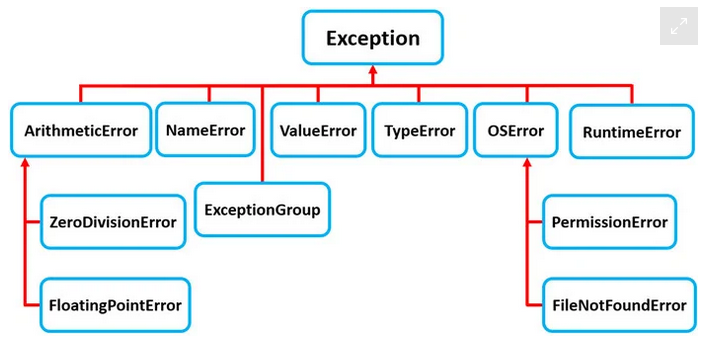
\includegraphics[width=260pt,height=200pt]{slike/class-exceptions.png}
	\caption{Hijerarhija najvažnijih klasa izuzetaka u Pajtonu.}
	\label{fig:exceptions}
\end{figure}

\bigskip

Pravilna upotreba izuzetaka predstavlja važan dio razvoja pouzdanih programa. Obradom izuzetaka moguće je spriječiti neočekivani prekid izvršavanja, korisniku pružiti jasne informacije o nastaloj grešci i povećati robusnost softvera.

\section{Rad sa datotekama}

Pomoću svojih ugrađenih funkcija, Pajton omogućuje jednostavan rad sa ulaznim i izlaznim datotekama. U nastavku dajemo pregled najčešće korište\-nih metoda.

\textit{Čitanje iz datoteke}. Koristimo funkciju \textit{open}(), koja ima dva argu\-menta -- naziv datoteke (ili putanja do datoteke) i način u kojem se otvara datoteka (npr. za čitanje, pisanje, dodavanje, itd.). Pogledajmo sljedeći primjer: 
\begin{minted}{python}
# Otvaranje fajla za citanje
file = open("datoteka.txt", "r")
# Citanje sadrzaja iz fajla 
sadrzaj = file.read()
# Zatvaranje fajla
file.close()
# Ispisivanje sadrzaja fajla 
print(sadrzaj)
\end{minted}

Dakle, prvo otvaramo datoteku  \texttt{datoteka.txt} samo za čitanje. Zatim čitamo sadržaj datoteke koristeći metodu \textit{read}() i čuvamo ga u varijabli \textit{sadrzaj}. Konačno, zatvaramo datoteku pomoću metode \textit{close}() i ispisujemo sadržaj datoteke. 



\textit{Pisanje u fajl}. Za pisanje u datoteku koristimo funkciju \textit{open}(), koja otvara fajl sa određenim nazivom, ali ovaj put sa načinom ``\textit{w}" (eng. \textit{write}), čime se dopušta pisanje u fajl. Pogledajmo sljedeći primjer.
\begin{minted}{python}
# Otvaranje fajla za pisanje
file = open("datoteka.txt", "w")
# Pisanje teksta u datoteku
file.write("Zdravo!")
#  Zatvaranje fajla 
file.close()
\end{minted}


\textit{Dodavanje u fajl}. Da biste dodali sadržaj u postojeći sadržaj datoteke, otvaramo fajl sa načinom ``\textit{a}" (eng. \textit{append}), a potom pomoću funkcije \textit{write}() upisujemo novi sadržaj na postojeći. 

Napomenimo da je dobra praksa zatvoriti datoteku nakon što zavr\-šite rad sa njom, kako bismo izbjegli bilo kakve potencijalne probleme sa oštećenjem datoteke ili gubitkom podataka. Praksa je da se rad u fajlovima odvija pod \textit{try}-\textit{except} blokom. Klase izuzetaka koje se u tim slučajevima mogu koristiti su: \texttt{FileNotFoundError} i \texttt{OSError}. 

% Upis json, csv, ispis itd. 

\subsection{Modul Json}

Modul \texttt{json} se koristi  za enkodiranje i dekodiranje podataka sa i u JSON format (eng. \textit{Java Script Object Notation}) formatu. JSON je  široko raspro\-stranjen format za razmjenu podataka, ljudima jednostavan za čitanje i pisanje, a mašinama za raščlanjivanje i generisanje.\\

Modul \texttt{json} nudi dvije glavne metode za rad sa JSON podacima:


\begin{itemize}
	\item json.\textit{dump}() -- koristi se za enkodiranje pajton objekata u JSON format i njegovo spremanje u objekat  datoteka.
	\item json.\textit{loads}() -- koristi se za dekodiranje JSON niza u pajtonov objekat (obično heš mapa).
\end{itemize}

Pogledajmo i jedan primjer upotrebe \texttt{json} modula. 

\begin{minted}{python}
	import json
	
	# Pajton objekat
	objekat = {'ime': 'Mirko', 'godine': 30, 'grad': 'Banja Luka'}
	# Enkoduj objekat u JSON string
	json_string = json.dumps(objekat)
	# Dekodiraj JSON string nazad u pajtonov objekat (dict)
	dekodiran_objekat = json.loads(json_string)
	
	print(type(json_string))   # <class 'str'>
	print(type(dekodiran_objekat))   # <class 'dict'>
	print(dekodiran_objekat)    # {'ime': 'Mirko', 'godine': 30,
		                        # 'grad': 'Banja Luka'}
\end{minted}


Primijetite da funkcija \textit{dumps}() pretvara pajtonov objekat u string (kodiranje), dok funkcija \textit{loads}() radi obrnutu akciju, od stringa pravi pajtonov objekat (enkodiranje). 

\section{Regularni izrazi}

Regularni izraz (engl. \textit{regular expression}, skraćeno \textit{regex}) predstavlja šablon za opisivanje i pretraživanje tekstualnih nizova. Drugim riječima, regularni izraz definiše skup stringova koji zadovoljavaju određena sintaksna pravila.

Osnovna svrha regularnih izraza jeste da se veliki skup stringova opiše na koncizan način, bez potrebe za njihovim pojedinačnim nabrajanjem. Na primjer, regularnim izrazom možemo opisati skup svih binarnih nizova ili skup riječi {\texttt{gray}, \texttt{grey}} koristeći samo jedan obrazac.

Regularni izrazi imaju široku primjenu u obradi teksta, pretraživanju podataka, validaciji korisničkog unosa, uređivačima teksta i alatima kao što je \texttt{grep} u operativnom sistemu Unix.

\subsection*{Osnovni koncepti regularnih izraza}

\begin{itemize}
	
	\item \textbf{Alternacija}
	
	Alternacija se označava simbolom \texttt{|} i predstavlja logičko ``ili''.
	
	Na primjer, 	$a|b|c $ opisuje skup stringova  $
	\{a,b,c\}.$
	
	\item \textbf{Grupisanje}
	
	Zagrade služe za grupisanje dijelova izraza i određivanje područja djelovanja operatora.
	
	Na primjer, $\texttt{gr}(a|e)\texttt{y}$ opisuje riječi $
	{\texttt{gray},\texttt{grey}}.
	$
	
	\item \textbf{Specijalni simboli i klase karaktera}
	
	\begin{itemize}
		
		\item \texttt{.} -- odgovara proizvoljnom karakteru;
		
		\item \texttt{[abc]} -- odgovara jednom od navedenih karaktera;
		
		\item \texttt{[a-z]} -- odgovara jednom malom slovu engleske abecede;
		
		\item \texttt{[A-Z]} -- odgovara jednom velikom slovu;
		
		\item \texttt{[a-zA-Z]} -- odgovara jednom slovu, bez obzira na veličinu;
		
		\item \texttt{\textbackslash d} -- odgovara jednoj cifri (ekvivalentno izrazu \texttt{[0-9]});
		
		\item \texttt{[\^{}abc]} -- odgovara bilo kojem karakteru osim navedenih;
		
		\item \texttt{\textbackslash w} -- odgovara slovu, cifri ili znaku \texttt{\_};
		
		\item \texttt{\textbackslash s} -- odgovara praznom znaku (razmak, tabulator, novi red);
		
		\item \texttt{\textbackslash n} -- odgovara znaku novog reda;
		
		\item \texttt{\textbackslash t} -- odgovara tabulatoru;
		
		\item \texttt{\textbackslash b} -- odgovara granici riječi.
		
	\end{itemize}
	
	\item \textbf{Kvantifikatori}
	
	Kvantifikatori određuju koliko puta se može pojaviti izraz koji im neposredno prethodi.
	
	\begin{itemize}
		
		\item \texttt{?} -- prethodni izraz pojavljuje se 0 ili 1 put;
		
		\item \texttt{*} -- prethodni izraz pojavljuje se 0 ili više puta;
		
		\item \texttt{+} -- prethodni izraz pojavljuje se 1 ili više puta;
		
		\item \texttt{{m,n}} -- prethodni izraz pojavljuje se najmanje $m$, a najviše $n$ puta.
		
	\end{itemize}
	
\end{itemize}

\subsection*{Primjeri}

\paragraph{Registarske tablice}

Pretpostavimo da registarska oznaka ima oblik:$
\texttt{A12-B-345}$

tj. jedno veliko slovo, dvije cifre, povlaku, jedno veliko slovo, novu povlaku i tri cifre.

Odgovarajući regularni izraz je: $
\texttt{[A-Z]\textbackslash d{2}-[A-Z]-\textbackslash d{3}}$

\paragraph{Datum u formatu DD.MM.GGGG.}

Ako se dan i mjesec uvijek zapisuju sa dvije cifre (npr. \texttt{01.02.2025.}), odgovarajući regularni izraz je: $
\texttt{(\textbackslash d{2})\textbackslash.(\textbackslash d{2})\textbackslash.(\textbackslash d{4})\textbackslash.} $

Ovaj izraz opisuje dvije cifre za dan, dvije cifre za mjesec i četiri cifre za godinu, razdvojene tačkama.

\bigskip

Regularni izrazi predstavljaju veoma moćan alat za obradu tekstualnih podataka. Iako njihova sintaksa na prvi pogled može djelovati složeno, pravilnom kombinacijom osnovnih operatora moguće je veoma precizno opisati i prepoznati složene obrasce u tekstu.

\subsection{Modul Re}

Modul \texttt{re} je ugrađeni Pajtonov modul namijenjen radu sa regularnim izrazima. Omogućava definisanje, pretraživanje i obradu tekstualnih obrazaca (\textit{patterna}), pa predstavlja jedan od najvažnijih alata za manipulaciju tekstualnim podacima.

Da bismo koristili funkcionalnosti ovog modula, potrebno ga je prvo uključiti naredbom:

\begin{minted}{python}
	import re
\end{minted}

Neke od najčešće korištenih funkcija modula \texttt{re} su:

\begin{itemize}
	
	\item \texttt{search(pattern, string)}
	
	Pretražuje string \texttt{string} i pronalazi prvo pojavljivanje obrasca \texttt{pattern}. Ukoliko se obrazac pronađe, funkcija vraća objekat podudaranja (\textit{match object}); u suprotnom vraća vrijednost \texttt{None}.
	
	\item \texttt{match(pattern, string)}
	
	Provjerava da li se obrazac \texttt{pattern} nalazi na samom početku stringa. Ako postoji podudaranje, vraća odgovarajući objekat podudaranja.
	
	\item \texttt{sub(pattern, replacement, string)}
	
	Zamjenjuje sva pojavljivanja obrasca \texttt{pattern} u stringu \texttt{string} novim tekstom \texttt{replacement}.
	
	\item \texttt{split(pattern, string)}
	
	Razdvaja string na dijelove koristeći obrazac \texttt{pattern} kao separator i vraća listu dobijenih podstringova.
	
	\item \texttt{findall(pattern, string)}
	
	Pronalazi sva podudaranja obrasca u stringu i vraća ih u obliku liste.
	
\end{itemize}

U nastavku je prikazan jednostavan primjer korištenja funkcije \texttt{search()}.

\begin{minted}{python}
	import re
	
	# Definisanje obrasca
	
	pattern = r'\b\w+'
	
	# Tekst koji pretražujemo
	text = 'Hello, World!'
	# Pretraga
	match = re.search(pattern, text)
	# Ispis prvog pronađenog podudaranja
	print(match.group())
\end{minted}

Izlaz programa je:

\begin{minted}{text}
	Hello
\end{minted}

Posmatrajmo detaljnije regularni izraz

\begin{minted}{python}
	r'\b\w+'
\end{minted}

Njegove komponente imaju sljedeće značenje:

\begin{itemize}
	\item \texttt{\textbackslash b} označava granicu riječi;
	\item \texttt{\textbackslash w} označava slovo, cifru ili znak \texttt{\_};
	\item \texttt{+} označava jedno ili više uzastopnih pojavljivanja prethodnog obrasca.
\end{itemize}

Dakle, izraz \texttt{\textbackslash b\textbackslash w+} odgovara prvoj riječi u tekstu, odnosno prvom nizu uzastopnih alfanumeričkih znakova koji počinje na granici riječi.

Napomenimo da se u primjeru koristi zapis

\begin{minted}{python}
	r'...'
\end{minted}

koji predstavlja tzv. \textit{raw string}. Kod ovakvog zapisa znak \texttt{\textbackslash} se ne tretira kao početak specijalne sekvence, što pojednostavljuje pisanje regularnih izraza i smanjuje mogućnost greške.

\section{Moduli Sys i Getopt}

\subsection*{Pokretanje programa iz komandne linije}

Pajton skripta se može pokrenuti iz terminala naredbom:

\begin{minted}{bash}
	python myscript.py arg1 arg2
\end{minted}

ili, na sistemima gdje je instalirano više verzija Pajtona,

\begin{minted}{bash}
	python3 myscript.py arg1 arg2
\end{minted}

Pri tome je:

\begin{itemize}
	\item \texttt{myscript.py} naziv skripte;
	\item \texttt{arg1}, \texttt{arg2}, \ldots argumenti komandne linije.
\end{itemize}

\subsection*{Modul Sys}

Modul \texttt{sys} omogućava pristup informacijama i funkcijama vezanim za Pajtonov interpreter i izvršno okruženje.

Neki od najčešće korištenih atributa i funkcija ovog modula su:

\begin{itemize}
	
	\item \texttt{sys.argv}
	
	Lista argumenata komandne linije. Element na poziciji \texttt{0} sadrži naziv skripte, dok ostali elementi predstavljaju argumente koje je korisnik proslijedio programu.
	
	\item \texttt{sys.path}
	
	Lista direktorijuma u kojima Pajton traži module za učitavanje.
	
	\item \texttt{sys.exit([kod])}
	
	Prekida izvršavanje programa i vraća izlazni kod operativnom sistemu. Ukoliko se kod ne navede, podrazumijeva se vrijednost 0.
	
	\item \texttt{sys.version}
	
	Vraća informaciju o verziji Pajtonovog interpretera.
	
	\item \texttt{sys.platform}
	
	Vraća oznaku platforme na kojoj se program izvršava.
	
\end{itemize}

Sljedeći primjer prikazuje korištenje atributa \texttt{argv}.

\begin{minted}{python}
	import sys
	
	if len(sys.argv) > 1:
	    print("Argumenti komandne linije su:")
	
	    for arg in sys.argv[1:]:
	        print(arg)
	 
	else:
	    print("Nema proslijeđenih argumenata.")
\end{minted}

Ako program pokrenemo naredbom

\begin{minted}{bash}
	python test.py arg1 arg2
\end{minted}

dobijamo izlaz

\begin{minted}{text}
	Argumenti komandne linije su:
	arg1
	arg2
\end{minted}

\subsection*{Modul Getopt}

Modul \texttt{getopt} služi za parsiranje opcija i argumenata komandne linije. Njegova funkcionalnost slična je istoimenoj funkciji dostupnoj u Unix operativnim sistemima.

Najvažnija funkcija modula je:

\begin{minted}{python}
	getopt.getopt(args, shortopts, longopts)
\end{minted}

gdje su:

\begin{itemize}
	\item \texttt{args} lista argumenata komandne linije;
	\item \texttt{shortopts} string koji definiše kratke opcije;
	\item \texttt{longopts} lista dugih opcija.
\end{itemize}

Funkcija vraća torku:

\begin{itemize}
	\item listu pronađenih parova \texttt{(opcija, vrijednost)};
	\item listu preostalih argumenata.
\end{itemize}

Na primjer, zapis

\begin{minted}{python}
	"hi:o:"
\end{minted}

definiše tri kratke opcije:

\begin{itemize}
	\item \texttt{-h} ne zahtijeva dodatnu vrijednost;
	\item \texttt{-i} zahtijeva vrijednost;
	\item \texttt{-o} zahtijeva vrijednost.
\end{itemize}

Dvotačka nakon oznake opcije označava da opcija mora imati pridruženu vrijednost.

Za duge opcije koristi se lista stringova:

\begin{minted}{python}
	["ifile=", "ofile="]
\end{minted}

Znak \texttt{=} na kraju naziva opcije označava da opcija zahtijeva argument.

\subsubsection*{Primjer}

\begin{minted}{python}
	import getopt
	import sys
	
	def main(argv):
	
	    inputfile = ""
	    outputfile = ""
	
	    try:
	        opts, args = getopt.getopt(
	            argv,
	            "hi:o:", ["ifile=", "ofile="]
	        )
	
	    except getopt.GetoptError:
	        print("test.py -i <inputfile> -o <outputfile>")
	        sys.exit(2)
	
	    for opt, arg in opts:
	
	        if opt == "-h": 
	            print("test.py -i <inputfile> -o <outputfile>")
	            sys.exit()
	
	        elif opt in ("-i", "--ifile"):
	            inputfile = arg
	
	        elif opt in ("-o", "--ofile"):
                outputfile = arg
	
	if __name__ == "__main__":
	main(sys.argv[1:])
\end{minted}

Program se može pokrenuti naredbom

\begin{minted}{bash}
	python3 test.py -i ulaz.txt -o izlaz.txt
\end{minted}

 
U slučaju da korisnik navede neispravne opcije ili izostavi obavezne argumente, aktivira se izuzetak \texttt{GetOptError}, koji se obrađuje u bloku \texttt{try-except}.

\bigskip

\textbf{Napomena.} U savremenim Pajton programima modul \texttt{argparse} uglavnom predstavlja preporučeni način za obradu argumenata komandne linije, jer nudi jednostavniju sintaksu, automatsko generisanje pomoći (\texttt{-h}) i bolju podršku za složenije aplikacije. Modul \texttt{getopt} je i dalje koristan za razumijevanje osnova parsiranja opcija i kompatibilnost sa Unix stilom komandne linije.


\section{Modul NumPy}

\texttt{NumPy} (skraćeno od \textit{Numerical Python}) predstavlja jednu od najvažnijih biblioteka za naučno i numeričko računarstvo u programskom jeziku Pajton. Razvio ju je Travis Oliphant 2005. godine, a značajan dio implementacije napisan je u jezicima \textit{C} i \textit{C++}.

Osnovna struktura podataka biblioteke NumPy je višedimenzionalni niz (\texttt{ndarray}), koji omogućava efikasan rad sa vektorima, matricama i višedimenzionalnim tenzorima.

Za razliku od Pajtonovih lista:

\begin{itemize}
	\item svi elementi NumPy niza moraju biti istog tipa;
	\item podaci se čuvaju u neprekidnom bloku memorije;
	\item aritmetičke operacije nad nizovima izvršavaju se veoma efikasno;
	\item zauzeće memorije je manje nego kod odgovarajućih lista.
\end{itemize}

Zbog toga su NumPy nizovi posebno pogodni za obradu velikih količina numeričkih podataka.

\begin{figure}[H]
	\centering
	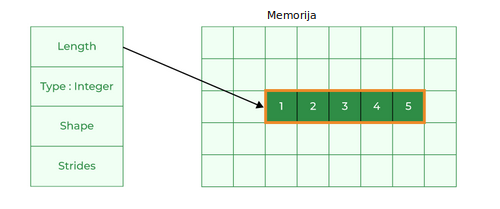
\includegraphics[width=280pt,height=140pt]{slike/numpy-array-memory.png}
	\caption{Pojednostavljen prikaz memorijske organizacije NumPy niza.}
	\label{fig:numpy_array}
\end{figure}

\subsection*{Kreiranje NumPy nizova}

Biblioteka se najčešće uključuje sljedećom naredbom:

\begin{minted}{python}
	import numpy as np
\end{minted}

Primjeri kreiranja jednodimenzionalnih i višedimenzionalnih nizova:

\begin{minted}{python}
	import numpy as np
	
	# Jednodimenzionalni niz
	
	arr = np.array([2, 4, 1, 10], dtype=np.int32)
	
	# Matrica (2D niz)
	
	matrica = np.array(
	[[2, 5],
	[1, 7]],
	dtype=np.int32
	)
	
	# Trodimenzionalni niz
	
	matrica3D = np.array(
	[
	[[2, 5], [1, 7]],
	[[2, 3], [5, 5]]
	],
	dtype=np.int32
	)
\end{minted}

Argument \texttt{dtype} određuje tip podataka koji se koristi za skladištenje elemenata. Neki od najčešćih tipova su:

\begin{center}
	\begin{tabular}{ll}
		\textbf{Tip} & \textbf{Značenje} \\ \hline
		\texttt{int32}, \texttt{int64} & cijeli brojevi \\
		\texttt{float32}, \texttt{float64} & realni brojevi \\
		\texttt{bool} & logičke vrijednosti \\
		\texttt{complex128} & kompleksni brojevi \\
		\texttt{str} & stringovi  \\ \hline \hline
	\end{tabular} 
\end{center}

\subsection*{Osnovne operacije}

\begin{itemize}
	
	\item \textbf{Pristup elementima}
	
	\begin{minted}{python}
		arr[2]           # element 1D niza
		matrica[1, 0]   # element matrice
	\end{minted}
	
	\item \textbf{Dimenzije niza}
	
	\begin{minted}{python}
		arr.shape
	\end{minted}
	
	Atribut \texttt{shape} vraća dimenzije niza.
	
	\item \textbf{Rezanje (slicing)}
	
	\begin{minted}{python}
		arr[1:5]
		arr[::2]
	\end{minted}
	
	\item \textbf{Kopiranje}
	
	\begin{minted}{python}
		kopija = arr.copy()
	\end{minted}
	
	\item \textbf{Promjena oblika}
	
	\begin{minted}{python}
		arr.reshape((2, 2))
	\end{minted}
	
	Broj elemenata mora ostati nepromijenjen.
	
	\item \textbf{Spajanje nizova}
	
	\begin{minted}{python}
		np.concatenate((arr1, arr2), axis=0)
	\end{minted}
	
	\item \textbf{Dijeljenje niza}
	
	\begin{minted}{python}
		np.array_split(arr, 3)
	\end{minted}
	
	\item \textbf{Pretraga elemenata}
	
	\begin{minted}{python}
		np.where(arr % 2 == 0)
	\end{minted}
	
	Vraća indekse elemenata koji zadovoljavaju dati uslov.
	
	\item \textbf{Sortiranje}
	
	\begin{minted}{python}
		np.sort(arr)
	\end{minted}
	
	\item \textbf{Filtriranje}
	
	\begin{minted}{python}
		arr = np.array([41, 42, 43, 44])
		
		filter_arr = arr > 42
		novi_arr = arr[filter_arr]
	\end{minted}
	
	Rezultat je niz:
	
	\begin{minted}{python}
		array([43, 44])
	\end{minted}
	
	\item \textbf{Kreiranje specijalnih nizova}
	
	\begin{minted}{python}
		np.zeros((3, 4))
		np.ones((2, 5))
	\end{minted}
	
\end{itemize}

\subsection*{Vektorizovane operacije}

Jedna od najvećih prednosti biblioteke NumPy jeste mogućnost izvođenja operacija nad cijelim nizovima bez eksplicitnog korištenja petlji.

\begin{minted}{python}
	a = np.array([1, 2, 3])
	b = np.array([4, 5, 6])
	
	c = a + b
\end{minted}

Rezultat je

\begin{minted}{python}
	array([5, 7, 9])
\end{minted}

Na isti način moguće je izvršavati množenje, dijeljenje, poređenja i brojne matematičke operacije nad kompletnim nizovima.

\subsection*{Memorijska organizacija}

Objekti biblioteke NumPy implementirani su klasom \texttt{ndarray}. Pored samih podataka, svaki objekat sadrži i određene metapodatke:

\begin{itemize}
	\item \texttt{dtype} -- tip elemenata niza;
	\item \texttt{ndim} -- broj dimenzija;
	\item \texttt{shape} -- dimenzije niza;
	\item \texttt{strides} -- broj bajtova koji je potrebno preskočiti da bi se došlo do sljedećeg elementa u određenoj dimenziji;
	\item \texttt{data} -- pokazivač na memorijsku oblast u kojoj se nalaze elementi niza.
\end{itemize}

Pošto su elementi smješteni u neprekidnom bloku memorije i imaju isti tip, pristup podacima i izvođenje numeričkih operacija znatno su efikasniji nego kod standardnih Pajtonovih lista.

\section{Modul Ctypes}

Modul \texttt{ctypes} omogućava pozivanje funkcija i korištenje tipova podataka definisanih u dijeljenim bibliotekama (\textit{shared libraries}) napisanim u jeziku \textit{C} ili drugim jezicima nižeg nivoa. Na taj način moguće je koristiti postojeći kôd napisan u jeziku \textit{C} direktno iz Pajtona, bez potrebe za ponovnom implementacijom.

Osnovni koraci za korištenje modula \texttt{ctypes} su sljedeći:

\begin{enumerate}
	\item Napisati program ili biblioteku u jeziku \textit{C}.

	\item Prevesti (\textit{kompajlirati}) program u dijeljenu biblioteku.
	
	Na Linux i macOS sistemima to se obično radi pomoću kompajlera \texttt{gcc}, dok se na Windows sistemima mogu koristiti Visual Studio ili MinGW.
	
	\item Učitati biblioteku u Pajton pomoću modula \texttt{ctypes}.
	
	\item Definisati tipove argumenata i povratne tipove funkcija koje želimo pozivati.
	
	\item Pozvati funkcije iz Pajtona kao da su obične Pajtonove funkcije.
\end{enumerate}

\subsection*{Primjer korištenja}

Pretpostavimo da želimo koristiti jednostavnu funkciju za sabiranje napisanu u jeziku \textit{C}.

\begin{minted}{C}
	// datoteka dodaj.c
	
	int saberi(int a, int b)
	{
		return a + b;
	}
\end{minted}

Na Linux sistemu biblioteku možemo kompajlirati naredbom:

\begin{minted}{bash}
	gcc -shared -fPIC -o libdodaj.so dodaj.c
\end{minted}

Nakon toga biblioteku učitavamo u Pajton:

\begin{minted}{python}
	import ctypes
	
	lib_dodaj = ctypes.CDLL("./libdodaj.so")
\end{minted}

Potom definišemo tipove argumenata i povratni tip funkcije:

\begin{minted}{python}
	saberi = lib_dodaj.saberi
	
	saberi.argtypes = [ctypes.c_int, ctypes.c_int]
	saberi.restype = ctypes.c_int
\end{minted}

Konačno, funkciju možemo pozvati na uobičajen način:

\begin{minted}{python}
	rezultat = saberi(2, 3)
	
	print(rezultat)   # Output: 5
\end{minted}

Modul \texttt{ctypes} automatski vrši konverziju između Pajtonovih i \textit{C} tipova podataka, što značajno pojednostavljuje komunikaciju između ova dva jezika.

\section{Pisanje prilagođenih modula}

Jedna od prednosti programskog jezika Pajton jeste mogućnost organizovanja koda u module. Modul predstavlja datoteku sa ekstenzijom \texttt{.py} koja sadrži funkcije, klase, konstante ili druge definicije koje se mogu koristiti u više programa.

Na primjer, pretpostavimo da želimo napraviti modul za osnovne matematičke operacije. Kreirajmo datoteku \texttt{mathOps.py} sa sljedećim sadržajem:

\begin{minted}{python}
	def add(x, y):
	    return x + y
	
	def subtract(x, y):
	    return x - y
	
	def multiply(x, y):
	    return x * y
	
	def divide(x, y):
	    if y == 0:
	        raise ValueError("Dijeljenje nulom nije dozvoljeno.")
	    return x / y
\end{minted}

Ovaj modul definiše četiri funkcije:

\begin{itemize}
	\item \texttt{add()} -- sabiranje dva broja;
	\item \texttt{subtract()} -- oduzimanje dva broja;
	\item \texttt{multiply()} -- množenje dva broja;
	\item \texttt{divide()} -- dijeljenje dva broja.
\end{itemize}

Nakon što je modul sačuvan, može se koristiti u drugoj Pajton skripti pomoću naredbe \texttt{import}:

\begin{minted}{python}
	import mathOps
	
	print(mathOps.add(3, 4))
	# Output: 7
	print(mathOps.divide(10, 2))
	# Output: 5.0
	
\end{minted}

Ako pokušamo izvršiti dijeljenje nulom:

\begin{minted}{python}
	mathOps.divide(10, 0)
\end{minted}

aktiviraće se izuzetak:

\begin{minted}{python}
	ValueError: Dijeljenje nulom nije dozvoljeno.
\end{minted}

Korištenje modula omogućava bolju organizaciju programa, veću ponovnu upotrebljivost koda i jednostavnije održavanje većih projekata. U praksi se složeni programi gotovo uvijek organizuju kao skup međusobno povezanih modula.

\section{Postavljanje korisnički kreiranih modula na PyPI repozitorij}

PyPI (\textit{Python Package Index}) predstavlja centralni repozitorijum paketa napisanih u programskom jeziku Pajton. Objavljivanjem paketa na PyPI-u omogućava se njegovo jednostavno distribuiranje i instaliranje od strane drugih korisnika.

Da bismo objavili vlastiti paket na PyPI-u, potrebno je izvršiti nekoliko koraka.

Prije svega, potrebno je kreirati korisnički nalog na zvaničnoj PyPI stranici:

\begin{center}
	\texttt{https://pypi.org/account/register/}
\end{center}

Nakon registracije preporučuje se kreiranje API tokena koji služi za sigurnu autentifikaciju prilikom postavljanja paketa na PyPI.

\subsection*{Priprema paketa}

Pretpostavimo da imamo paket pod nazivom \texttt{modul1}. U korijenskom direktorijumu projekta kreiramo datoteku \texttt{pyproject.toml} koja sadrži osnovne metapodatke o paketu:

\begin{minted}{toml}
	[build-system]
	requires = ["setuptools>=61.0"]
	build-backend = "setuptools.build_meta"
	
	[project]
	name = "modul1"
	version = "0.0.1"
	authors = [
	{name = "Mirko Mirković"}
	]
	description = "Primjer korisničkog modula"
	dependencies = [
	"numpy",
	"pandas"
	]
\end{minted}

Ova datoteka definiše naziv paketa, verziju, autora, opis i zavisnosti koje će biti automatski instalirane zajedno sa paketom.

\subsection*{Instalacija potrebnih alata}

Za izgradnju i objavljivanje paketa potrebno je instalirati nekoliko pomoćnih alata:

\begin{minted}{bash}
	pip install build twine
\end{minted}

Paket \texttt{build} služi za kreiranje distribucionih datoteka, dok \texttt{twine} omogućava njihovo postavljanje na PyPI.

\subsection*{Kreiranje distribucije}

Distribucione datoteke kreiraju se naredbom:

\begin{minted}{bash}
	python -m build
\end{minted}

Nakon uspješnog izvršavanja ove naredbe kreira se direktorijum \texttt{dist} koji sadrži:

\begin{itemize}
	\item izvornu distribuciju (\texttt{.tar.gz});
	\item binarnu distribuciju (\texttt{.whl}).
\end{itemize}

\subsection*{Objavljivanje paketa}

Prije objavljivanja preporučuje se provjera ispravnosti generisanih datoteka:

\begin{minted}{bash}
	twine check dist/*
\end{minted}

Paket se zatim objavljuje naredbom:

\begin{minted}{bash}
	twine upload dist/*
\end{minted}

Prilikom objavljivanja koristi se korisničko ime \texttt{\_\_token\_\_} i prethodno generisani PyPI API token.

Nakon uspješnog postavljanja paket postaje dostupan svim korisnicima putem PyPI repozitorijuma.

\subsection*{Instalacija objavljenog paketa}

Objavljeni paket može se instalirati standardnom \texttt{pip} naredbom:

\begin{minted}{bash}
	pip install modul1
\end{minted}

Nakon instalacije paket se može koristiti u bilo kojem Pajton programu:

\begin{minted}{python}
	import modul1
\end{minted}

Objavljivanje paketa na PyPI-u predstavlja standardni način distribucije Pajton softvera i omogućava jednostavno dijeljenje biblioteka sa širom programerskom zajednicom.

\section{Kompajliranje i izvršavanje programa}

U ovom odjeljku ukratko opisujemo način na koji se izvršava program napisan u programskom jeziku Pajton, kao i osnovne principe organizacije memorije tokom rada programa.

\subsection{Stek i hip memorija}

Tokom izvršavanja programa operativni sistem i Pajtonov interpreter koriste različite dijelove memorije. Među njima posebno su važni \textit{stek} (\textit{stack}) i \textit{hip} (\textit{heap}).

\textbf{Stek} predstavlja memorijski prostor koji se koristi za čuvanje informacija o aktivnim pozivima funkcija. Svaki put kada se pozove funkcija, na steku se kreira novi zapis (engl. \textit{stack frame}) koji sadrži informacije potrebne za izvršavanje te funkcije.

Kada funkcija završi rad, njen zapis se uklanja sa steka. Zbog toga kažemo da je stek privremena memorijska struktura čiji je životni vijek vezan za trajanje poziva funkcije.

Posmatrajmo sljedeći primjer:

\begin{minted}{python}
	def func():
	    a = 10
	    b = []
	    c = "abc"
\end{minted}

Prilikom poziva funkcije \texttt{func()} kreira se novi zapis na steku. U njemu se čuvaju reference na objekte označene imenima \texttt{a}, \texttt{b} i \texttt{c}. Nakon završetka funkcije ove reference se uklanjaju iz memorije steka.

Međutim, stvarni objekti na koje reference pokazuju uglavnom se nalaze u drugom dijelu memorije koji se naziva \textbf{hip} (\textit{heap}).

Hip predstavlja dinamički dio memorije namijenjen skladištenju objekata čija veličina može biti poznata tek tokom izvršavanja programa. Gotovo svi Pajton objekti, uključujući liste, rječnike, skupove, torke, stringove i numeričke vrijednosti, smještaju se u hip memoriju.

Na primjer:
\begin{minted}{python}
	a = [0] * 10
\end{minted}

U ovom slučaju lista od deset elemenata kreira se u hip memoriji, dok varijabla \texttt{a} predstavlja referencu na taj objekat.

Za razliku od jezika \textit{C} i \textit{C++}, gdje programer često mora ručno upravljati memorijom, u Pajtonu se dodjeljivanje i oslobađanje memorije obavlja automatski. Interpreter vodi računa o tome kada je potrebno kreirati novi objekat i kada se memorija može osloboditi.

\subsection{Sakupljanje otpadaka}

Pajton koristi mehanizam poznat pod nazivom \textit{garbage collection} (sakupljanje otpadaka). Njegov zadatak je automatsko uklanjanje objekata koji više nisu dostupni nijednom dijelu programa.

Osnovni mehanizam zasniva se na brojanju referenci. Svaki objekat vodi evidenciju o broju aktivnih referenci koje pokazuju na njega. Kada broj referenci postane jednak nuli, objekat se može ukloniti iz memorije.

Pored toga, Pajton koristi i dodatni algoritam za otkrivanje kružnih referenci, odnosno situacija u kojima dva ili više objekata međusobno referenciraju jedni na druge, ali više nisu dostupni ostatku programa.

Zahvaljujući ovim mehanizmima, programer u većini slučajeva ne mora voditi računa o ručnom oslobađanju memorije, što značajno pojednostavljuje razvoj softvera i smanjuje mogućnost pojave memorijskih grešaka.

\subsection{Proces prevođenja i izvršavanja programa}

Iako se Pajton često opisuje kao interpretirani programski jezik, proces izvršavanja programa zapravo uključuje i fazu prevođenja izvornog koda. Zbog toga se može reći da je Pajton istovremeno i kompajlirani i interpretirani jezik.

Proces izvršavanja programa sastoji se od nekoliko osnovnih koraka.

\begin{enumerate}
	
	\item \textbf{Leksička analiza}
	
	Izvorni kôd najprije prolazi kroz leksički analizator koji ga razlaže na elementarne cjeline nazvane \textit{tokeni}. Primjeri tokena su ključne riječi, identifikatori, operatori, literali i interpunkcijski simboli.
	
	\item \textbf{Sintaksna analiza}
	
	Dobijeni tokeni prosljeđuju se parseru koji na osnovu gramatičkih pravila jezika gradi \textit{apstraktno sintaksno stablo} (\textit{Abstract Syntax Tree -- AST}). AST predstavlja hijerarhijsku strukturu programa i služi kao osnova za naredne faze prevođenja.
	
	\item \textbf{Generisanje bajtkoda}
	
	Na osnovu AST strukture Pajton generiše \textit{bajtkod} (\textit{bytecode}), koji predstavlja međureprezentaciju nezavisnu od operativnog sistema i procesorske arhitekture.
	
	Generisani bajtkod može biti sačuvan u datotekama sa ekstenzijom \texttt{.pyc}.
	
	\item \textbf{Izvršavanje bajtkoda}
	
	Bajtkod izvršava Pajtonova virtuelna mašina (\textit{Python Virtual Machine -- PVM}). Virtuelna mašina čita instrukcije bajtkoda i izvršava ih jednu po jednu, upravljajući memorijom, objektima i tokom programa.

\end{enumerate}

Pojednostavljen prikaz procesa izvršavanja prikazan je na Slici~\ref{fig:comp_interpreting}.

\begin{figure}[H]
	\centering
	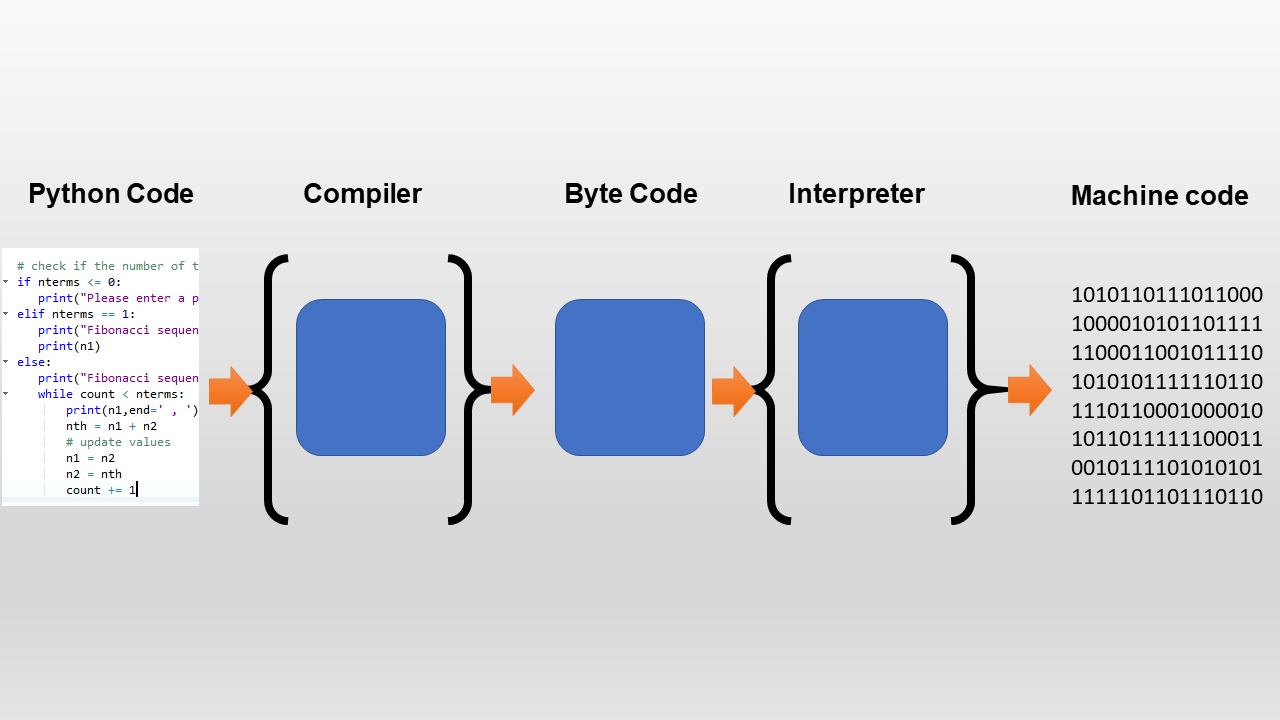
\includegraphics[width=350pt,height=170pt]{slike/python-code-copiler-machine-code.png}
	\caption{Pojednostavljen prikaz procesa prevođenja i izvršavanja Pajton programa.\protect\footnotemark}
	\label{fig:comp_interpreting}
\end{figure}

\footnotetext{Slika preuzeta sa: \texttt{https://www.astateofdata.com/python-programming/can-python-be-compiled/}}

\subsection{Pajtonova virtuelna mašina}

Pajtonova virtuelna mašina (PVM) predstavlja centralnu komponentu izvršnog okruženja jezika Pajton. Njena osnovna uloga jeste izvršavanje bajtkoda generisanog tokom procesa prevođenja izvornog programa.

Najvažnije funkcije PVM-a su:

\begin{itemize}
	
	\item \textbf{Prenosivost programa}
	
	Bajtkod je nezavisan od konkretne hardverske platforme. Zbog toga se isti Pajton program može izvršavati na različitim operativnim sistemima bez izmjene izvornog koda.
	
	\item \textbf{Izvršavanje bajtkoda}
	
	PVM interpretira instrukcije bajtkoda i prevodi ih u odgovarajuće operacije nad objektima i memorijom.
	
	\item \textbf{Dinamičko tipiziranje}
	
	Pošto se tipovi objekata određuju tokom izvršavanja programa, PVM upravlja svim provjerama i operacijama vezanim za tipove podataka.
	
	\item \textbf{Upravljanje memorijom}
	
	PVM koristi mehanizme brojanja referenci i sakupljanja otpadaka (\textit{garbage collection}) kako bi automatski oslobađala memoriju koja više nije potrebna.
	
	\item \textbf{Podrška za module i biblioteke}
	
	PVM omogućava učitavanje i korištenje velikog broja ugrađenih i eksternih biblioteka pomoću naredbe \texttt{import}.

\end{itemize}

Treba napomenuti da standardna implementacija Pajtona (CPython) koristi interpretaciju bajtkoda. Postoje i druge implementacije, kao što su PyPy, Jython i IronPython, koje koriste drugačije tehnike izvršavanja i optimizacije programa.

Na osnovu svega navedenog može se zaključiti da Pajton prvo prevodi izvorni kôd u bajtkod, a zatim taj bajtkod izvršava pomoću virtuelne mašine. Zbog toga se često kaže da je Pajton hibrid između kompajliranih i interpretiranih programskih jezika.


\section*{Zadaci}
%regularni izrazi:
\begin{enumerate}
    %%https://adriann.github.io/programming_problems.html
    
    \item Implementi igru pogađanja u kojoj korisnik treba da pogodi skriveni broj. Nakon pogađanja, program izvještava korisnika da li je njegov broj velik ili mali (ili je pogođen). Na kraju ispisati broj  pokušaja iz kojeg je korisnik pogodio skriveni broj. Računa se jedan pokušaj ukoliko se unese isti broj više puta uzastopno.
    
    
	\item Napisati program koji računa sljedeću sumu  
	
	$$ 4 \cdot \sum_{k=1}^{10^6}(-1)^{k-1} \frac{1}{2k-1}= 4 \cdot (1-1/3 + 1/5-1/7+1/9-1/11 \ldots).$$
	
	\item Napisati funkciju koja kombinira dvije liste naizmjenično uzimajući elemente jedne pa druge liste, Npr. za $[a,b,c], [5, 6, 7]$ generišemo listu $[a,5,b,6,c,7]$.
	
	\item Napisati funkciju koja pomijera elemente liste za $k$ elemenata. Npr. lista  $[1,2,3,4,5,6]$ rotirana za $k=2$ je data sa $[3,4,5,6,1,2]$. Riješiti zadatak bez kreiranja kopije liste. 
	
	\item Napisati funkciju koja uzima broj i vraća listu njegovih brojeva. Npr. za broj $2342$ treba vratiti listu $[2,3,4,2]$.
	
	\item Napisati funkciju koja uzima listu brojeva,   bazu $b_1$ u kojoj se brojevi liste interpretiraju, te ciljnu bazu $b_2$.  Kao rezultat vratiti listu brojeva konvertujući svaki od brojeva početne liste u bazu $b_2$. Npr. za listu $[21,10,01]$ u bazi $b_1 = 3$ pretvaramo u listu brojeva po bazi $b_2=10$, pri čemu vraćamo listu $[7,3, 1]$.
	
	\item Napišite funkciju koja množi dvije matrice. Vratiti grešku (koristiti izuzetke) ukoliko su dimenzije matrica nekompatibilne.  
	 
	\item Napisati regularni izraz koji prepoznaje registarske tablice. Testirati primjenu tog paterna uz pomoć modula \texttt{re}.
	
	\item Napisati regularni izraz koji prepoznaje email adrese. Testirati primjenu tog paterna uz pomoć modula \texttt{re}.
	
	\item Napisati regularni izraz koji prepoznaje realne brojeve (u decimalnom ili eksponencijalnom zapisu). Testirati primjenu uz pomoć modula \texttt{re}.
	
	
	\item Kreirati datoteku \textit{apsolventi}.txt i popuniti je podacima gdje je u svakom redu data
	informacija o studentu apsolventu u formi: 
	 $$<Ime\_prezime>, <datum\_upisa\_na\_fakultet>, <godine\_starosti>$$ 
	
	Datum se zadaje u formi $<$broj$>$.$<$broj$>$.$<$broj$>$. Napisati skriptu koja se pokreće sa terminala čiji su argumenti komandne linije:
	\begin{itemize}
		\item  	\textit{i}: koja zadaje ulaznu datoteku (apsolutna putanja) koja treba da bude učitana u
	program;
	     \item \textit{o}: koja zadaje izlaznu datoteku (apsolutna putanja) u kojoj se čuvaju rezultati	izvršavanja programa;
	     \item  \textit{z}: koji zadaje zadatak koji treba da bude izvršen i obuhvata sljedeći opseg vrijednosti: 
	     \begin{itemize}
	     	\item  1: U izlaznoj datoteci treba da se ispišu svi apsolventi stariji od 25 godina.
             \item 2: U izlaznoj datoteci treba da se ispišu svi apsolventi koji su upisali fakultet u periodu od 01.01.2014.\ do 01.01.2015. godine.
	         \item 3: U izlaznoj datoteci treba da se ispiše sortiran niz (koristiti merge sort) studenata po godini starosti.
	         \item 4: U izlaznoj datoteci treba da se ispiše za svakog studenta koliko godina studira/je studirao.
	        \item Za ostale inpute javiti poruku o neispravnoj opciji (unosu). Koristiti izuzetke.
	         \end{itemize}
       \end{itemize}
	\textit{Napomena}. Studenta učitati uz pomoć regularnih izraza. Dakle, prazan karakter predstavlja 
	invarijantna vrijednost što se postiže konstru\-kcijom odgovarajućeg regularnog izraza koji parsira  sadržaj svakog reda  datoteke.
	
   \item Kreirati datoteku \emph{pretplatnik.txt} i popuniti je podacima gdje je u svakom redu
   data informacija o pretplatniku u formi
   
   $$<Ime\_prezime>, <datum\_ugovora>, <cijena\_usluge>$$
   
   Datum se zadaje u formi $<$broj$>$.$<$broj$>$.$<$broj$>$, a cijena je decimalni broj. Napisati 
   skriptu koja se pokreće sa terminala sa sljedećim argumentima komandne linije:
   \begin{itemize}
   	\item \textit{i}: koja zadaje ulaznu datoteku (apsolutna putanja) koja treba da bude učitana
   u program;
   \item \textit{o}: koja zadaje izlaznu datoteku (apsolutna putanja) koja treba da sačuva
   rezultate izvršavanja programa;
    \item \textit{z}: koji zadaje zadatak koji treba da bude izvršen i obuhvata sljedeće vrijednosti:
    \begin{itemize}
    	\item  1: U izlaznoj datoteci treba da se ispišu svi korisnici koji koriste usluge čija je  cijena veća od 15.4 KM. Elimini\-sati duplikate. 
        \item 2: U izlaznoj datoteci treba da se ispišu svi pretplatnici koji su potpisali ugovor u periodu od 01.01.2022.\ do 15.01.2023. godine.
        \item  3: U izlaznoj datoteci treba da se ispiše zbir svih cijena za usluge koje koristi svaki od pretplatnika. 
        \item 4: U izlaznoj datoteci treba da se ispišu sortirane cijene od najmanje do  najveće.
        \item Za ostale inpute javiti poruku o neispravnoj opciji  (unosu) koristeći izuzetke.
         \end{itemize}
   \end{itemize}
   \textit{Napomena}. Pretplatnika učitati uz pomoć regularnih izraza. Npr., smatra se da je unos Marko
   Markovic, $20.2.2022, 8,4$ isti kao Marko Markovic, $20.\ \ 2.2022, 8,\ \ 4$, itd.  Dakle, prazan karakter predstavlja 
   invarijantnu vrijednost što se postiže konstrukcijom odgovarajućeg regularnog izraza koji parsiraju  sadržaj svakog reda iz datoteke.
\end{enumerate}
 
\chapter{Osnovne algoritamske paradigme}

Prilikom rješavanja računarskih problema često se koriste određeni obrasci razmišljanja i pristupi konstruisanju algoritama. Takvi pristupi nazivaju se \textit{algoritamske paradigme}. Svaka paradigma predstavlja opšti metod za dizajniranje algoritama i može se primijeniti na širok spektar problema.

Prije nego što pređemo na algoritamske paradigme, vrijedi pomenuti da postoje i različite \textit{programske paradigme}, odnosno stilovi programiranja koji određuju način organizacije i pisanja programskog k\^oda. Najpoznatije programske paradigme su:

\begin{itemize}
	\item \textit{imperativno programiranje}, zasnovano na sekvencijalnom izvršavanju naredbi;
	\item \textit{funkcionalno programiranje}, koje naglasak stavlja na funkcije i transformaciju podataka;
	\item \textit{logičko programiranje}, zasnovano na pravilima i zaključivanju;
	\item \textit{objektno orijentisano programiranje}, koje modeluje probleme pomoću objekata i njihovih međusobnih interakcija.
\end{itemize}

Savremeni programski jezici često podržavaju više paradigmi istovremeno, omogućavajući programerima da odaberu pristup koji najbolje odgovara problemu koji rješavaju.

Kada je riječ o algoritmima, različiti problemi zahtijevaju različite strategije dizajniranja. Upravo te strategije nazivamo algoritamskim paradigmama. U nastavku navodimo najvažnije među njima.

\begin{itemize}

	\item \textbf{Rekurzivni algoritmi}
	
	Zasnivaju se na razlaganju problema na manje podprobleme iste prirode. Rješenje se dobija rekurzivnim pozivanjem algoritma sve dok se ne dostigne jedan od baznih slučajeva.
	
	\item \textbf{Algoritmi grube sile} (eng. \textit{brute force})
	
	Zasnivaju se na ispitivanju svih mogućih rješenja dok se ne pronađe ispravno ili optimalno rješenje. Jednostavni su za implementaciju, ali često imaju visoku vremensku složenost.
	
	\item \textbf{Podijeli pa zavladaj} (eng. \textit{divide-and-conquer})
	
	Problem se dijeli na više manjih nezavisnih podproblema koji se rješavaju odvojeno, nakon čega se njihova rješenja kombinuju u rješenje originalnog problema.% Klasični primjeri su Sortiranje spajanjem i Brzo sortiranje.
	
	\item \textbf{Pohlepni algoritmi} (eng. \textit{greedy algorithms})
	
	U svakom koraku donose lokalno najbolje moguće rješenje, uz pretpostavku da će takav izbor dovesti do globalno optimalnog rješenja. Karakterišu ih jednostavnost i mala potrošnja memorije, ali ne garantuju optimalnost za većinu problema.
	
	\item \textbf{Dinamičko programiranje} (eng. \textit{dynamic programming})
	
	Problem se razlaže na podprobleme koji se međusobno preklapaju. Rezultati već riješenih podproblema memorišu se i ponovo koriste, čime se izbjegava višestruko računanje istih vrijednosti.
	
	\item \textbf{Vraćanje unazad} (eng. \textit{backtracking})
	
	Rješenje se gradi postepeno. Kada se ustanovi da trenutno parcijalno rješenje ne može dovesti do validnog rješenja, algoritam se vraća na prethodni korak i pokušava alternativni izbor.
	
	\item \textbf{Randomizirani algoritmi}
	
	U proces odlučivanja uvode element slučajnosti. Često se koriste za ubrzavanje algoritama ili za efikasno rješavanje problema velikih dimenzija.
	
\end{itemize}

Važno je naglasiti da ove paradigme nisu međusobno isključive. U praksi se veoma često kombinuju kako bi se dobili efikasniji algoritmi za rješavanje složenih računarskih problema. U nastavku knjige detaljnije ćemo proučiti nekoliko najvažnijih algoritamskih paradigmi i njihove primjene.\\

%ISHODI UCENJA:
\section*{Ishodi učenja}

Nakon uspješnog savladavanja sadržaja ove glave student će biti u stanju da:

\begin{itemize}
	\item objasni princip rekurzije i razlikuje rekurzivni od iterativnog pristupa rješavanju problema;
	
	\item primijeni algoritme grube sile i osnovne algoritme pretraživanja	na jednostavne probleme;
	
	\item objasni i primijeni paradigmu podijeli pa zavladaj pri razlaganju problema na manje podprobleme;
	
	\item koristi paradigmu vraćanja unazad za sistematsko pretraživanje prostora rješenja i odbacivanje nedopustivih parcijalnih rješenja;
	
	\item objasni princip pohlepnih algoritama i prepozna situacije u kojima lokalno najbolji izbor može voditi ka kvalitetnom ili optimalnom rješenju;
	
	\item primijeni dinamičko programiranje kroz definisanje podproblema,
	rekurentnih relacija i memorisanje već izračunatih rezultata te procijeni
	vremensku i prostornu složenost dobijenog algoritma.
\end{itemize}



\section{Rekurzivni algoritmi}

Rekurzija predstavlja jednu od osnovnih algoritamskih paradigmi. Sama riječ potiče od latinske riječi \textit{recurrere}, što znači \emph{vraćati se}. U programiranju se funkcija naziva \textit{rekurzivnom} ukoliko u svom tijelu direktno ili indirektno poziva samu sebe.

Osnovna ideja rekurzije sastoji se u tome da se problem postepeno svodi na manje podprobleme iste prirode. Svaki rekurzivni poziv funkcije obrađuje jednostavniju instancu problema, sve dok se ne dostigne jedan od unaprijed definisanih \textit{baznih slučajeva}. Bazni slučajevi predstavljaju trivijalne situacije za koje je rješenje poznato i služe za zaustavljanje rekurzivnog procesa.

Pravilno definisanje baznih slučajeva od ključnog je značaja. Ukoliko oni ne postoje ili nisu dostižni, rekurzivni pozivi će se nastaviti beskonačno, što na kraju dovodi do prekoračenja memorije rezervisane za stek.

\subsection{Jednostavan primjer rekurzije}

Posmatrajmo problem određivanja $n$-tog parnog broja. Neka funkcija $f(n)$ označava $n$-ti parni broj u skupu nenegativnih cijelih brojeva $\mathbb{N}_0$.

Pošto je prvi parni broj jednak nuli, definišemo $
f(0)=0.$  Svaki naredni parni broj za dva je veći od prethodnog, pa važi rekurzivna relacija $f(n)=f(n-1)+2, n\geq 1.$ Na primjer, $f(3)=f(2)+2=f(1)+2+2=f(0)+2+2+2=6.$  Dakle, za izračunavanje vrijednosti $f(3)$ potrebno je izračunati $f(2)$, zatim $f(1)$ i konačno bazni slučaj $f(0)$. Nakon dostizanja baznog slučaja, rekurzija se vraća unazad i sukcesivno računa vrijednosti $f(1)$, $f(2)$ i $f(3)$.

Rekurzivna implementacija ove funkcije u Pajtonu izgleda ovako:

\begin{minted}{python}
	def even(n):
	    if n == 0:
	        return 0
	
	    return even(n - 1) + 2

	n = int(input("Unesite broj: "))
	print(even(n))
\end{minted}

\textbf{Vremenska složenost.}
Funkcija izvršava tačno $n$ rekurzivnih poziva, pa je njena vremenska složenost jednaka $
O(n).$

Međutim, u ovom primjeru rekurzija nije neophodna jer se lako može izvesti zatvorena formula $f(n)=2n.$

\subsection{Rekurzivno računanje faktorijela}

Jedan od najpoznatijih primjera primjene rekurzije jeste računanje faktorijela prirodnog broja. Faktorijel broja $n$ se može definisati rekurzivno sa $n! = n \cdot \underbrace{(n-1) \cdot (n-2)\cdots 2 \cdot 1},$ tj. 

$$n! = n \cdot (n-1)!.$$

Bazni slučaj je $0! = 1.$ Implementacija računanja faktorijela broja rekurzivnim načinom bi izgledala ovako:

\begin{minted}{python}
	def fact(n):
	    if n == 0:
	        return 1

	    return n * fact(n - 1)
\end{minted}

Na primjer, za $n=5$ izvršava se sljedeći niz poziva: $fact(5)\rightarrow fact(4)\rightarrow fact(3)
\rightarrow fact(2)\rightarrow fact(1)\rightarrow fact(0).$

Nakon dostizanja baznog slučaja, rezultati se vraćaju unazad kroz stek poziva.

\begin{figure}[H]
	\centering
	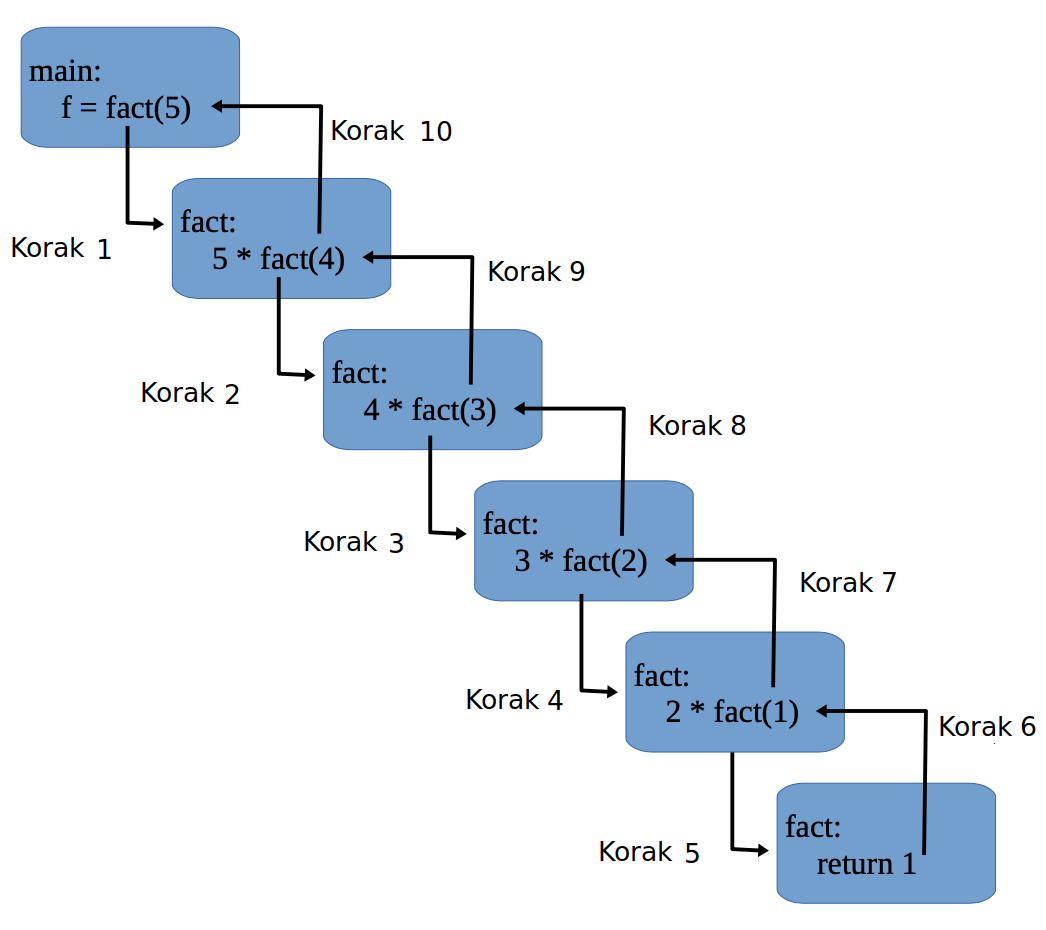
\includegraphics[width=220pt,height=160pt]{slike/factorial_recursion_tree.png}
	\caption{Drvo rekurzivnih poziva za funkciju faktorijela.}
	\label{fig:rec_tree}
\end{figure}

\textbf{Vremenska složenost.}
Broj rekurzivnih poziva proporcionalan je vrijednosti parametra $n$, pa je složenost $ O(n).$

\subsection{Prekoračenje steka}

Ako bazni slučaj nije pravilno definisan ili nije dostižan, rekurzija se neće završiti. Posmatrajmo sljedeći primjer:

\begin{minted}{python}
	def fact(n):
	
	    if n == 100:
	        return 1
	    return n * fact(n - 1)
\end{minted}

Ukoliko je početna vrijednost parametra manja od 100, funkcija će nastaviti da poziva samu sebe sa sve manjim vrijednostima argumenta i nikada neće dostići bazni slučaj. Posljedica je prekoračenje maksimalne dubine rekurzije i aktiviranje izuzetka:

\begin{minted}{python}
	RecursionError:
	maximum recursion depth exceeded
\end{minted}

Maksimalna dozvoljena dubina rekurzije može se provjeriti i po potrebi izmijeniti pomoću funkcija modula \texttt{sys}, iako se povećanje ove granice uglavnom ne preporučuje.

\section{Vrste rekurzije}

Rekurzivne funkcije mogu se klasifikovati na više načina.

\subsection*{Direktna i indirektna rekurzija}

Funkcija je \textit{direktno rekurzivna} ukoliko poziva samu sebe. Funkcija je \textit{indirektno rekurzivna} ukoliko poziva drugu funkciju koja, direktno ili indirektno, ponovo poziva prvu funkciju.

\begin{minted}{python}
	
	# Direktna rekurzija
	
	def direktna():
	    direktna()
	
	# Indirektna rekurzija
	def funkcija1():
	     funkcija2()
	
	def funkcija2():
	    funkcija1()
\end{minted}

\subsection*{Repna i nerepna rekurzija}

Rekurzija se naziva \textit{repnom} (eng. \textit{tail recursion}) ukoliko je rekurzivni poziv posljednja operacija koja se izvršava u funkciji.

\begin{minted}{python}
	def countdown(n):
	
	    if n == 0:
	        return
	    return countdown(n - 1)
	
\end{minted}

U suprotnom govorimo o \textit{nerepnoj rekurziji}. Na primjer:

\begin{minted}{python}
	def fact(n):
	
	    if n == 0:
	        return 1
	
	    return n * fact(n - 1)
	
\end{minted}

Pošto se nakon povratka iz rekurzivnog poziva još uvijek izvršava operacija množenja, funkcija \texttt{fact()} predstavlja primjer nerepne rekurzije.

Iako neki programski jezici optimizuju repnu rekurziju, standardna implementacija Pajtona (CPython) ne primjenjuje ovu optimizaciju. Zbog toga duboke rekurzije mogu dovesti do povećane potrošnje memorije i pojave izuzetka \texttt{RecursionError}.

 
\subsection{Rekurzivni i iterativni pristup: poređenje}

Svaki rekurzivni algoritam može se implementirati i u iterativnom obliku, korištenjem petlji i odgovarajućih pomoćnih struktura podataka. Iako oba pristupa imaju istu računarsku moć, među njima postoje značajne razlike.

\begin{itemize}
	\item Rekurzija se završava dostizanjem baznog slučaja, dok se iteracija završava kada uslov petlje postane netačan.
	
	\item Rekurzija je zasnovana na pozivima funkcija, dok se iteracija zasniva na petljama (\texttt{for} i \texttt{while}).
	
	\item Svaki rekurzivni poziv zauzima dodatni prostor u memoriji steka, dok iterativni algoritmi uglavnom zahtijevaju manje dodatne memorije.
	
	\item Rekurzivna rješenja često su kraća i bliža matematičkoj formulaciji problema, dok iterativna rješenja mogu biti nešto duža što se tiče k\^oda, ali su obično efikasnija.	
\end{itemize}

Rekurzivni programi najčešće zahtijevaju više memorije od ekvivalentnih iterativnih programa, jer se informacije o svakom pozivu funkcije čuvaju u steku sve do dostizanja baznog slučaja. Takođe, dodatno vrijeme izvršavanja troši se na pozivanje funkcija i povratak rezultata.

S druge strane, rekurzija često omogućava elegantnije i preglednije implementacije. Neki problemi prirodno imaju rekurzivnu strukturu, kao što su obilazak stabala, problem Hanojskih kula, generisanje kombinacija i permutacija, te različiti algoritmi zasnovani na paradigmi \emph{podijeli pa zavladaj}. U takvim situacijama rekurzivni pristup često predstavlja intuitivnije rješenje.

\subsection{Primjene rekurzije}

Rekurzija se koristi u brojnim oblastima informatike i programiranja. %Neke od najvažnijih primjena su:

\begin{enumerate}
	
	\item \textbf{Pretraga stabala i grafova}: Rekurzija se prirodno koristi za obilazak hijerarhijskih struktura podataka kao što su stabla i grafovi. Primjeri su algoritmi DFS (eng. \emph{Depth-First Search}) i različiti obilaci binarnih stabala.
	
	\item \textbf{Algoritmi sortiranja}: Mnogi poznati algoritmi sortiranja koriste rekurziju. Primjeri su Brzo sortiranje i Sort spajanjem, koji problem sortiranja razlažu na manje podprobleme i zatim kombinuju njihova rješenja.
	
	\item \textbf{Generisanje fraktala}:  Brojni fraktalni objekti mogu se generisati primjenom rekurzivnih pravila. Jedan od najpoznatijih primjera je Mandelbrotov skup.
	
	\begin{figure}[H]
		\centering
		
\includegraphics[width=100pt,height=80pt]{slike/mandelbrot.png}
		\caption{Mandelbrotov skup.}
	\end{figure}
	
	\item \textbf{Algoritmi vraćanja unazad}:  Ovi algoritmi postepeno grade rješenje problema. Kada se ustanovi da trenutno parcijalno rješenje ne može dovesti do validnog konačnog rješenja, algoritam se vraća na prethodno stanje i pokušava drugu mogućnost.
	
	\item \textbf{Dinamičko programiranje i memoizacija}:	Memoizacija predstavlja tehniku pohranjivanja prethodno izračunatih rezultata podproblema kako bi se izbjeglo njihovo ponovno računanje. Ova tehnika se često koristi zajedno sa rekurzijom i predstavlja osnovu mnogih algoritama dinamičkog programiranja.
\end{enumerate}

U nastavku ćemo ilustrovati primjenu rekurzije na nekoliko konkretnih problema.

\begin{example}
	Pretpostavimo da se populacija zečeva razvija prema sljedećem pravilu. Par zečeva tokom prvog mjeseca života ne daje potomstvo. Počevši od drugog mjeseca života, svaki par na kraju svakog mjeseca proizvede jedan novi par zečeva. Koliko će novih parova zečeva biti nakon 12 mjeseci?
\end{example}

\begin{solution}
	
	Broj novorođenih parova po mjesecima formira niz $$[0,1,1,2,3,5,8,13,21,\ldots].$$
	
	Poznat je kao Fibonačijev niz. Ako sa $f(n)$ označimo broj novorođenih parova na kraju $n$-tog mjeseca, tada važi rekurzivna relacija
	$ f(n)=f(n-1)+f(n-2), n\geq 2,$ uz bazne slučajeve $f(0)=0, f(1)=1. $
	
\end{solution}

Odgovarajuća rekurzivna implementacija glasi:

\begin{minted}{python}
	def fib(n):
	    if n == 0:
	        return 0
	
	    if n == 1:
	        return 1
	
	    return fib(n - 1) + fib(n - 2)
\end{minted}

U svakom netrivijalnom koraku funkcija generiše dva nova rekurzivna poziva. Zbog toga se broj poziva vrlo brzo povećava sa rastom vrijednosti parametra $n$.

\textbf{Vremenska složenost.}  Za funkciju vrijedi rekurentna relacija $T(n)=T(n-1)+T(n-2)+O(1).$

Rješenje ove rekurencije ima eksponencijalni rast, pa je vremenska složenost $
T(n)=O(\varphi^n),$ gdje je $\varphi=\frac{1+\sqrt{5}}{2}\approx 1.618$ zlatni presjek. U literaturi se često koristi i grublja ocjena $ T(n)=O(2^n).$

Ovaj primjer pokazuje da rekurzija sama po sebi ne garantuje efikasan algoritam. U narednim poglavljima vidjećemo kako se primjenom memoizacije i dinamičkog programiranja složenost računanja Fibonačijevih brojeva može smanjiti sa eksponencijalne na linearnu.


%fib_rec.jpeg
\begin{figure}[H]
	\centering
	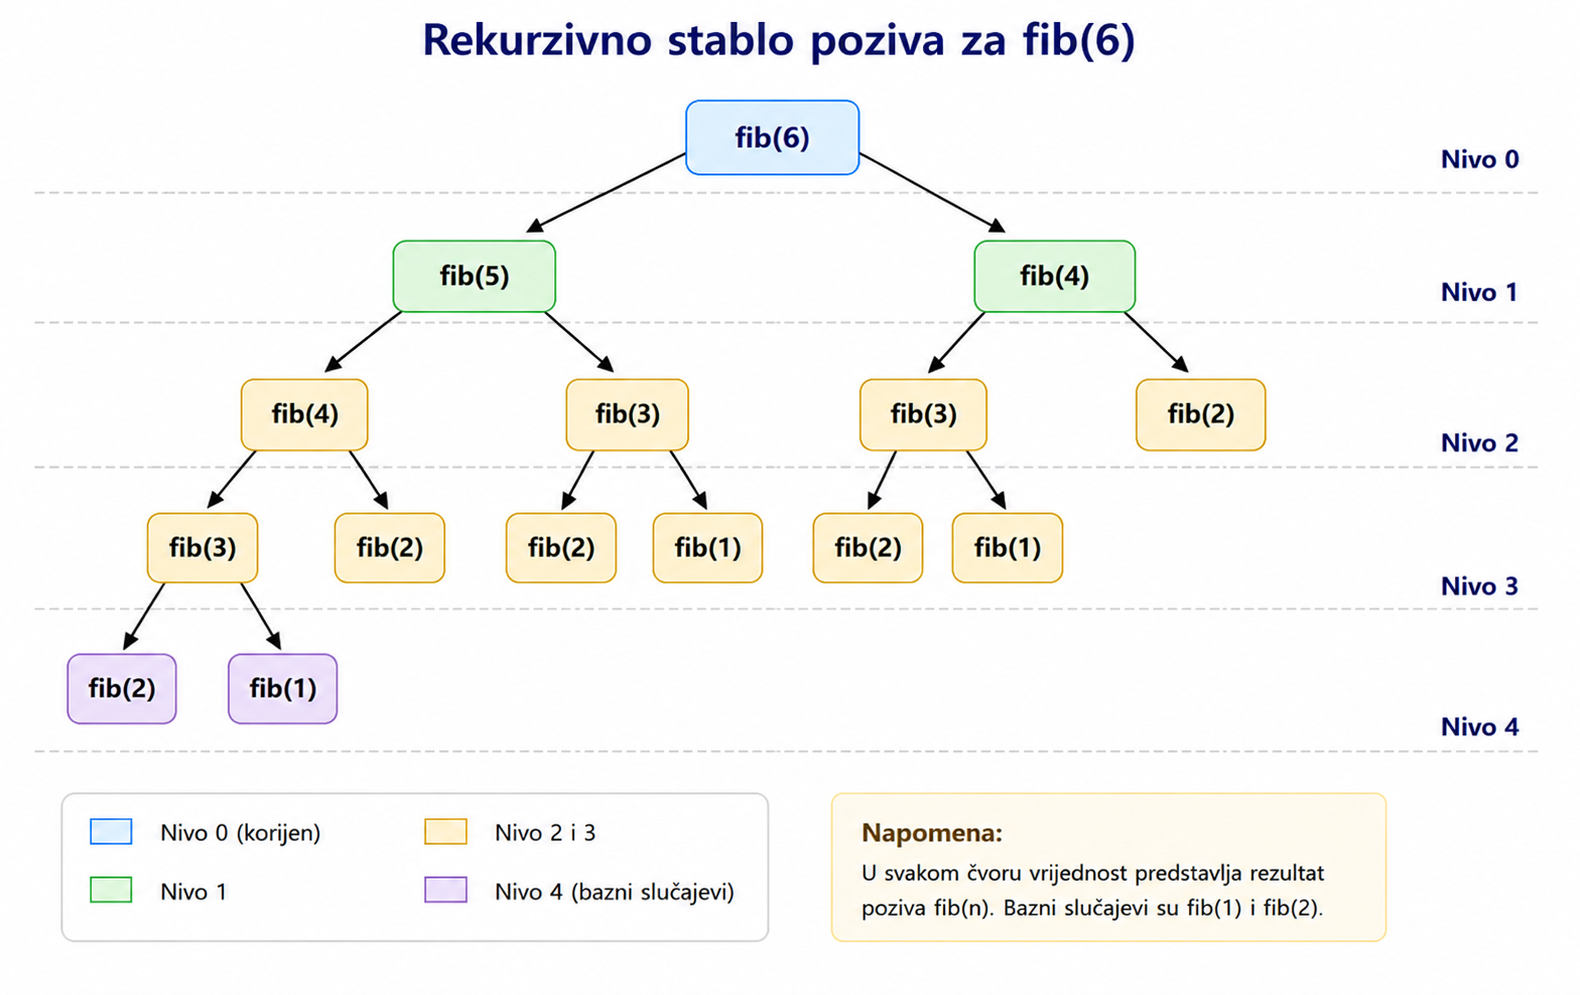
\includegraphics[width=250pt,height=140pt]{slike/fib_rec.png} 
	\label{fig:rec_fib}
	\caption{Drvo rekurzije za \texttt{fib} rekurzivni metod.}
\end{figure}


\begin{example}
	\textbf{(\emph{Problem Hanojskih kula})}
	
	Data su tri štapa i $n$ diskova različitih dimenzija. Svi diskovi su inicijalno složeni na jednom štapu ($A$), pri čemu se manji diskovi nalaze iznad većih. Cilj je premjestiti kompletnu kulu diskova na drugi štap ($C$), koristeći treći štap ($B$) kao pomoćni.
	
	Pri tome moraju biti zadovoljena sljedeća pravila:
	
	\begin{itemize}
		\item U jednom potezu dozvoljeno je premjestiti samo jedan disk.
		
		\item Disk se uvijek uzima sa vrha jednog štapa i postavlja na vrh drugog štapa.
		
		\item Veći disk nikada ne smije biti postavljen na manji disk.
		
	\end{itemize}
	
	Odrediti minimalan broj poteza potreban za premještanje svih diskova sa štapa $A$ na štap $C$.
\end{example}

\begin{solution}
	
	Najprije razmotrimo slučaj sa dva diska ($n=2$). Pretpostavimo da se oba diska nalaze na štapu $A$, a da ih želimo premjestiti na štap $C$.
	
	Rješenje se sastoji od tri poteza:
	
	\begin{enumerate}
		\item manji disk se premješta sa štapa $A$ na štap $B$;
		\item veći disk se premješta sa štapa $A$ na štap $C$;
		\item manji disk se premješta sa štapa $B$ na štap $C$.
	\end{enumerate}
	
	Posmatrajmo sada slučaj sa tri diska ($n=3$), prikazan na Slici~\ref{fig:tower}.
	
	\begin{figure}[H]
		\centering
		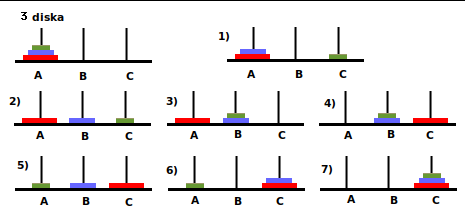
\includegraphics[width=270pt,height=150pt]{slike/tower.png}
		\caption{Problem Hanojskih kula za $n=3$ diska.}
		\label{fig:tower}
	\end{figure}
	
	Rješenje se dobija sljedećim redoslijedom poteza:
	
	\begin{enumerate}
		\item najmanji disk se premješta sa štapa $A$ na štap $C$;
		\item srednji disk se premješta sa štapa $A$ na štap $B$;
		\item najmanji disk se premješta sa štapa $C$ na štap $B$;
		\item najveći disk se premješta sa štapa $A$ na štap $C$;
		\item najmanji disk se premješta sa štapa $B$ na štap $A$;
		\item srednji disk se premješta sa štapa $B$ na štap $C$;
		\item najmanji disk se premješta sa štapa $A$ na štap $C$.
	\end{enumerate}
	
	Ukupno je potrebno sedam poteza.\\
	
	Da bismo riješili opšti slučaj, označimo sa $T(n)$ minimalan broj poteza potreban za premještanje $n$ diskova sa štapa $A$ na štap $C$, koristeći štap $B$ kao pomoćni.
	
	Bazni slučaj je jednostavan: $	T(1)=1.$  Za proizvoljno $n>1$, najprije je potrebno premjestiti gornjih $n-1$ diskova sa štapa $A$ na štap $B$, koristeći štap $C$. Za to je potrebno $T(n-1)$ poteza.  Nakon toga najveći disk ostaje sam na štapu $A$ i može se direktno premjestiti na štap $C$ u jednom potezu.
	
	Preostaje da se $n-1$ diskova sa štapa $B$ rekurzivno premjesti na štap $C$, za šta je ponovo potrebno $T(n-1)$ poteza.  	Prema tome, ukupan broj poteza zadovoljava rekurentnu relaciju $ T(n)=T(n-1)+1+T(n-1),$  odnosno	$	T(n)=2T(n-1)+1, 	T(1)=1.$ Prethodni postupak opisuje rekurzivnu formulaciju problema Hanojskih kula.
	
	Rješavanjem navedene rekurencije dobija se zatvorena forma $T(n)=2^n-1.$	Dakle, minimalan broj poteza potreban za premještanje $n$ diskova iznosi 	$2^n-1.$ Na primjer, za $n=3$ dobijamo $T(3)=2^3-1=7,$ što se slaže sa prethodno izvedenim rješenjem.
\end{solution}

Implementacija rekurzivnog pristupa problema Hanojskih kula je data sljedećim k\^odom. 

\begin{minted}{python}
	 
	def TowerOfHanoi(n , izvor, cilj, pomocni):
	    if n==1:
	        print ("Pomaknite disk 1 sa štapa ", izvor," \ 
	        na štap ", cilj)
	        return
	    TowerOfHanoi(n-1, izvor, pomocni, cilj)
	    print ("Pomakni disk ",n," sa štapa ", izvor," na štap  \ 
	     ", cilj) #pomijeranje najvećeg štapa
	    TowerOfHanoi(n-1, pomocni, cilj, izvor)
	
	#instanca:
	n = 4 #broj diskova
	TowerOfHanoi(n, 'A','C','B')
\end{minted} 

\textbf{Vremenska kompleksnost}. Vrlo lako dobijamo eksplicitnu funkciju koja odgovara   rekurzivnoj relaciji problema: $T(n)= 2  T(n-1) + 1 = 2 \cdot ( 2 \cdot T(n-2) + 1) + 1 = \cdots = 2^{n-2} + 2^{n-1} + \cdots + 2 + 1 = 2^n -1.$
Rekurzija se izvrašava u eksponencijalnom $O(2^n)$ vremenu.   
\end{solution}	
 

\begin{example}
  
     Sortiranje umetanjem (\emph{Insertion Sort}) predstavlja jednostavan algoritam
     sortiranja koji niz gradi postepeno, održavajući   jedan njegov dio sortiranim. Ideja algoritma sastoji se u tome da se  svaki novi element umetne na odgovarajuću poziciju unutar već sortiranog dijela niza. Niz koji se sastoji od jednog elementa se smatra sortiranim. 
 \end{example}
 
\begin{solution}
    Algoritam sortiranja umetanjem može se prirodno formulirati i rekurzivno.
     Neka je dat niz
 \[
 A = (a_0,a_1,\ldots,a_{n-1})
 \]
 od $n$ elemenata koje je potrebno sortirati u neopadajućem poretku.
 
 Rekurzivna formulacija zasniva se na sljedećem zapažanju. Pretpostavimo da smo
 već sortirali prvih $n-1$ elemenata niza:
 \[
 (a_0,a_1,\ldots,a_{n-2}).
 \]
 Tada je za sortiranje kompletnog niza dovoljno posljednji element
 $a_{n-1}$ umetnuti na odgovarajuću poziciju unutar već sortiranog prefiksa.
 
 Prema tome, algoritam se sastoji od dvije osnovne faze:
 
 \begin{enumerate}
 	\item rekurzivno sortirati prvih $n-1$ elemenata niza;
 	\item umetnuti posljednji element $a_{n-1}$ na odgovarajuću poziciju
 	unutar sortiranog prefiksa.
 \end{enumerate}
 
 Bazni slučaj nastupa kada niz sadrži najviše jedan element. Takav niz je već
 sortiran, pa nije potrebno izvršavati dodatne operacije.
 
 Pretpostavimo sada da su elementi
 \[
 a_0,a_1,\ldots,a_{n-2}
 \]
 već sortirani. Vrijednost $a_{n-1}$ privremeno čuvamo u promjenljivoj
 \texttt{key}. Zatim se, počevši od elementa $a_{n-2}$, krećemo unazad kroz
 sortirani dio niza. Svaki element koji je veći od vrijednosti \texttt{key}
 pomjera se za jednu poziciju udesno. Kada pronađemo prvi element koji nije
 veći od \texttt{key}, vrijednost \texttt{key} umećemo neposredno iza njega.
 
 Na ovaj način nakon završetka postupka prvih $n$ elemenata niza nalazi se u sortiranom poretku.
\end{solution}
% Pseudokod rekurzivnog algoritma dat je Algoritmom~\ref{alg:recursive-insertion-sort}.
 
%PSEUDOKOD:
\begin{minted}[fontsize=\footnotesize]{python}
	def RecursiveInsertionSort(A, n):
	    if n <= 1:
	        return
	
	    # Rekurzivno sortiramo prvih n-1 elemenata
    	RecursiveInsertionSort(A, n - 1)
	
	    # Umetanje posljednjeg elementa
	    key = A[n - 1]
	    j = n - 2
	
	    while j >= 0 and A[j] > key:
	        A[j + 1] = A[j]
	        j = j - 1
	
	    A[j + 1] = key
\end{minted}


 
 Na primjer, posmatrajmo niz
 \[
 A=[7,3,5,2].
 \]
 Rekurzivni algoritam najprije sortira prefiks dužine $3$,
 odnosno niz $
 [7,3,5],$
 koji nakon sortiranja postaje $
 [3,5,7].$ 
 Preostaje umetanje posljednjeg elementa $2$. Pošto je $2$ manje od svih
 elemenata sortiranog prefiksa, elementi $7$, $5$ i $3$ pomjeraju se za jednu
 poziciju udesno, nakon čega se vrijednost $2$ postavlja na početak niza.
 Dobijamo konačno sortirani niz $
 [2,3,5,7].$
 
 \paragraph{Ispravnost algoritma.} Ispravnost rekurzivnog algoritma možemo pokazati indukcijom po veličini
 niza $n$. Za $n=1$ niz sadrži samo jedan element i trivijalno je sortiran.  Pretpostavimo sada da algoritam ispravno sortira svaki niz od $n-1$
 elemenata. Pri pozivu algoritma za niz od $n$ elemenata, rekurzivni poziv
 sortira njegovih prvih $n-1$ elemenata. Nakon toga posljednji element
 $a_{n-1}$ umeće se na odgovarajuću poziciju unutar sortiranog prefiksa,
 pri čemu se svi elementi veći od njega pomjeraju za jednu poziciju udesno.
 Prema tome, nakon umetanja svih $n$ elemenata nalazi se u neopadajućem
 poretku. Time je pokazano da algoritam ispravno sortira niz proizvoljne
 dužine $n$.
 
 \paragraph{Vremenska složenost.}
 Neka je $T(n)$ vrijeme potrebno za sortiranje niza od $n$ elemenata.
 
 Algoritam najprije rekurzivno sortira prvih $n-1$ elemenata, što zahtijeva
 vrijeme $T(n-1)$. Nakon toga posljednji element umeće se u već sortirani
 prefiks.
 
 U najgorem slučaju posljednji element je manji od svih prethodnih elemenata.
 Tada je potrebno pomjeriti svih $n-1$ elemenata za jednu poziciju udesno.
 Zbog toga operacija umetanja zahtijeva $\Theta(n)$ vremena.
 
 Dobijamo rekurentnu relaciju
 \[
 T(n)=T(n-1)+\Theta(n),
 \]
 uz bazni slučaj
 \[
 T(1)=\Theta(1).
 \]
 
 Razvijanjem rekurzije dobijamo
 \[
 \begin{aligned}
 	T(n)
 	&= T(n-1)+\Theta(n)\\
 	&= T(n-2)+\Theta(n-1)+\Theta(n)\\
 	&\;\;\vdots\\
 	&= T(1)+\Theta(2)+\Theta(3)+\cdots+\Theta(n).
 \end{aligned}
 \]
 
 Kako vrijedi
 \[
 1+2+\cdots+n=\frac{n(n+1)}{2},
 \]
 slijedi
 \[
 T(n)=\Theta(n^2).
 \]
 
 Prema tome, vremenska složenost rekurzivnog algoritma sortiranja umetanjem
 u najgorem slučaju iznosi ${\Theta(n^2)}.$
 
 Najgori slučaj nastupa kada je početni niz sortiran u opadajućem poretku.
 Tada se pri svakom umetanju trenutni element mora pomjeriti preko svih
 prethodno obrađenih elemenata.
 
 U najboljem slučaju niz je već sortiran. Tada se pri svakom rekurzivnom
 nivou izvršava samo jedno poređenje prije nego što se utvrdi da se
 posljednji element već nalazi na odgovarajućoj poziciji. Rekurentna relacija
 tada ima oblik
 \[
 T_{\mathrm{best}}(n)
 =
 T_{\mathrm{best}}(n-1)+\Theta(1),
 \]
 odakle slijedi
 \[
 T_{\mathrm{best}}(n)=\Theta(n).
 \]
 
 Prosječna vremenska složenost algoritma iznosi $
 \Theta(n^2).$
 
 \paragraph{Prostorna složenost.}
 Sama operacija umetanja koristi samo konstantan broj dodatnih promjenljivih.
 Međutim, zbog rekurzivne implementacije na steku se istovremeno može nalaziti
 do $n$ aktivnih poziva funkcije. Zbog toga dodatna prostorna složenost
 rekurzivnog algoritma iznosi $\Theta(n)$.
 
 Kod standardne iterativne implementacije sortiranja umetanjem ovaj dodatni
 trošak ne postoji, pa je njena prostorna složenost $\Theta(1)$.
 
 Sortiranje umetanjem nije efikasno za velike nizove zbog kvadratne prosječne
 i najgore vremenske složenosti. Ipak, algoritam ima nekoliko važnih
 prednosti. Jednostavan je za implementaciju, ne zahtijeva dodatnu memoriju
 za čuvanje elemenata i veoma je efikasan za male ili skoro sortirane nizove.
 
 Rekurzivna formulacija posebno je korisna sa pedagoškog stanovišta, jer
 jasno pokazuje način na koji se problem veličine $n$ može svesti na problem
 istog tipa veličine $n-1$. Time sortiranje umetanjem predstavlja jednostavan
 primjer primjene rekurzivnog načina razmišljanja na problem sortiranja.

\section{Algoritmi grube sile}

Algoritmi grube sile predstavljaju jednu od najjednostavnijih algoritamskih paradigmi za rješavanje računarskih problema. Osnovna ideja ove paradigme jeste sistematsko ispitivanje svih mogućih rješenja dok se ne pronađe rješenje koje zadovoljava postavljene uslove ili dok se ne odredi najbolje rješenje prema zadanom kriterijumu.

Iako je riječ o jednostavnom pristupu, algoritmi grube sile imaju značajnu ulogu u algoritamskom dizajnu. Često predstavljaju polaznu tačku za razvoj efikasnijih algoritama, a za probleme manjih dimenzija mogu dati zadovoljavajuća rješenja.

U svakodnevnom životu primjer algoritma grube sile je pokušaj otključavanja brave kada ne znamo koji ključ odgovara. U tom slučaju isprobavamo jedan po jedan ključ sve dok ne pronađemo odgovarajući. Slično tome, ukoliko ne znamo orijentaciju USB priključka, pokušavamo jednu mogućnost, a zatim drugu.

Paradigma grube sile može se koristi za:

\begin{itemize}
	\item probleme pretraživanja,
	\item probleme zadovoljenja ograničenja (SAT problemi),
	\item probleme optimizacije,
	\item verifikaciju ispravnosti složenijih algoritama.
\end{itemize}

\begin{example}(\textbf{Problem najbližeg para tačaka}) Neka je dat skup od $n$ tačaka u prostoru $\mathbb{R}^m$:
	
	\[
	S=\{\mathbf{x}_1,\mathbf{x}_2,\ldots,\mathbf{x}_n\}.
	\]
	
	Potrebno je pronaći dvije tačke iz skupa $S$ čija je međusobna Euklidova udaljenost najmanja.
	
\end{example}

\begin{solution}
	
	Pristup grube sile podrazumijeva izračunavanje udaljenosti između svakog para tačaka iz skupa $S$. Tokom izvršavanja algoritma pamtimo najmanju do sada pronađenu udaljenost i odgovarajući par tačaka.
	
	Jedna moguća implementacija prikazana je u nastavku.
	
	\begin{minted}{python}
		import math
		
		def min_dist_pair(S):
		
		    min_dist = float("inf")
		    point1 = None
		    point2 = None
		
		    for i in range(len(S)):
		        for j in range(i + 1, len(S)):
		            distance = math.dist(S[i], S[j])
		
		            if distance < min_dist:
		                min_dist = distance
		                point1 = S[i]
		                point2 = S[j]
		
		    return point1, point2, min_dist
		
	\end{minted}
	
\end{solution}

\textbf{Analiza složenosti.} Broj različitih parova tačaka jednak je $\binom{n}{2}=\frac{n(n-1)}{2}=O(n^2).$  Računanje Euklidove udaljenosti između dvije tačke u prostoru $\mathbb{R}^m$ se vrši u $O(m)$ vremenu. Kako je dimenzija prostora $m$ fiksna, ukupna vremenska složenost algoritma iznosi $O(n^2).$

\vspace{0.3cm}

\begin{example}
	(\textbf{Problem ruksaka}). 
	Neka je dato $n$ predmeta. Svaki predmet $i$ ima težinu $w_i$ i vrijednost $p_i$, za svaki $i=1,\ldots,n$. Takođe je dat ruksak kapaciteta $C$.\\
	Potrebno je odabrati predmete koje treba staviti u ruksak tako da njihova ukupna težina ne prelazi kapacitet ruksaka, a pri tome je ukupna vrijednost u ruksaku najveća moguća.

\end{example}

\begin{solution}
	
	Posmatrajmo sljedeću instancu problema.
	
	\begin{center}
		\begin{tabular}{ccc}
			\emph{Predmet} & \emph{Težina} & \emph{Vrijednost} \\ \hline
			1 & 2  & 20 \\
			2 & 5  & 30 \\
			3 & 10 & 50 \\
			4 & 5  & 10 \\ \hline \hline
		\end{tabular}
	\end{center}
	
	Neka je kapacitet ruksaka $C=16.$	Pristup grube sile sastoji se u generisanju svih mogućih podskupova skupa predmeta. Kako postoje četiri predmeta, ukupan broj mogućih rješenja jednak je $2^4 = 16.$
	
	Za svaki podskup izračunava se ukupna težina i ukupna vrijednost.
	
	\begin{center}
		\begin{tabular}{lcc}
			Rješenje & Ukupna težina & Ukupna vrijednost \\ \hline
			$\{1\}$ & 2 & 20  \\
			$\{2\}$ & 5 & 30  \\
			$\{3\}$ & 10 & 50  \\
			$\{4\}$ & 5 & 10  \\
			$\{1,2\}$ & 7 & 50  \\
			$\{1,3\}$ & 12 & 70  \\
			$\{1,4\}$ & 7 & 30  \\
			$\{2,3\}$ & 15 & 80  \\
			$\{2,4\}$ & 10 & 40  \\
			$\{3,4\}$ & 15 & 60 \\
			$\{1,2,3\}$ & 17 & nedopustivo  \\
			$\{1,2,4\}$ & 12 & 60  \\
			$\{1,3,4\}$ & 17 & nedopustivo  \\
			$\{2,3,4\}$ & 20 & nedopustivo  \\
			$\{1,2,3,4\}$ & 22 & nedopustivo  \\ \hline
		\end{tabular}
	\end{center}
	
	Iz tabele se vidi da optimalno rješenje odgovara skupu $\{2,3\},$ čija je ukupna težina $15$, a ukupna pridružena vrijednost $80$.
	
\end{solution}

Pošto se svaki predmet može ili nalaziti ili ne nalaziti u ruksaku, prostor rješenja odgovara skupu svih podskupova skupa $\{1,\ldots,n\}$. Broj mogućih rješenja jednak je $2^n.$

Zbog toga je vremenska složenost algoritma grube sile eksponencijalna, $O(2^n).$\\

Jedna moguća implementacija prikazana je u nastavku.

\begin{minted}[fontsize=\footnotesize]{python}
	best_fitness = 0
	
	# primjer instance
	N = 4
	w = [2, 5, 10, 5]
	p = [20, 30, 50, 10]
	C = 16
	
	def objective(solution):
	
 	    weight = 0
	    value = 0
	
	    for i in solution:
	        weight += w[i]
	        value += p[i]
	
	    if weight > C:
	        return float("-inf")
	    return value
	
	def knapsack_brute_force(solution):
	
	
	    global best_fitness
	    
	    best_fitness = max(
	        best_fitness,
	        objective(solution))
	
	    for i in range(N):
	
	        if len(solution) == 0:
	            knapsack_brute_force([i])
	
	        elif i > max(solution): #razbijanje simetrije
	            knapsack_brute_force(solution + [i])
	
	knapsack_brute_force([])
	print(best_fitness)   # 80
\end{minted}

Algoritmi grube sile obično nisu praktični za velike instance problema zbog eksponencijalnog ili polinomijalno visokog vremena izvršavanja. Ipak, oni imaju značajnu teorijsku vrijednost jer garantuju pronalaženje optimalnog rješenja i često predstavljaju osnovu za razvoj efikasnijih algoritama zasnovanih na paradigmi \emph{podijeli pa zavladaj}, dinamičkom programiranju, grananju i ograničavanju (eng. \emph{branch-and-bound}) ili metaheuristikama.


Kako primjećujemo na osnovu prethodne (rekurzivne) implementacije, svaki od  
rekurzivnih poziva, kojih je tačno $2^n$, poziva funkciju \texttt{objective}. Preciznije, kompleksnost pristupa brutalne sile je $O(2^n)$. Napomenimo da postoje efikasniji pristupi za rješavanje problema ruksaka. Među njima, izdvajamo metod dinamičkog programiranja, o kojem će biti više riječi u nastavku.


\section{Algoritmi pretraživanja}

Algoritmi pretraživanja predstavljaju grupu algoritama čiji je zadatak pronalaženje određenog elementa unutar strukture podataka. Rezultat pretrage najčešće je informacija da li traženi element postoji, a ukoliko postoji, vraća se njegova pozicija ili druga relevantna informacija o njemu.

Algoritmi pretraživanja imaju široku primjenu u računarstvu, od rada sa nizovima i listama do pretraživanja baza podataka, tekstualnih dokumenata i složenih struktura podataka.

U zavisnosti od načina organizacije podataka i strategije pretraživanja, algoritmi pretraživanja mogu se podijeliti u dvije osnovne kategorije:

\begin{itemize}
	\item \textit{Sekvencijalna pretraga} prolazi kroz elemente strukture jedan po jedan sve dok ne pronađe traženi element ili ne iscrpi cijelu strukturu. Najpoznatiji predstavnik ove grupe je \textit{linearna pretraga}.
	
	\item \textit{Intervalna pretraga} koristi dodatne informacije o organizaciji podataka, najčešće činjenicu da su podaci sortirani. Umjesto provjeravanja svih elemenata, prostor pretrage se postepeno smanjuje, čime se postiže znatno veća efikasnost. Najpoznatiji primjer je \textit{binarna pretraga}.

\end{itemize}

\subsection{Linearna pretraga}

Linearna pretraga (eng. \emph{linear search}) predstavlja najjednostavniji algoritam pretraživanja. Ideja algoritma je da se elementi strukture podataka obilaze redom, od početka prema kraju, sve dok se ne pronađe tražena vrijednost.

U slučaju da se traženi element pronađe, algoritam vraća njegov indeks. Ukoliko se dođe do kraja strukture bez pronalaska elementa, vraća se posebna vrijednost koja označava neuspješnu pretragu.

Iterativna implementacija linearne pretrage prikazana je u nastavku.

\begin{minted}{python}
	def search(arr, x):
	
	
	    for i in range(len(arr)):
	        if arr[i] == x:
	        return i
	
	    return -1
	
	arr = [2, 3, 1, 11, 10, 20]
	x = 10
	res = search(arr, x)
	
	if res == -1:
	    print("Element nije pronađen.")
	else:
	    print("Element je pronađen na indeksu", res)
\end{minted}

\textbf{Analiza složenosti.} U najgorem slučaju algoritam mora pregledati svih $n$ elemenata strukture podataka. Zbog toga je vremenska složenost linearne pretrage $O(n),$  gdje je $n$ broj elemenata u strukturi. Dodatna memorija koja se koristi tokom izvršavanja algoritma je konstantna, pa je prostorna složenost jednaka $O(1).$

\vspace{0.3cm}

Linearna pretraga može se implementirati i rekurzivno.

\begin{minted}{python}
	def linear_search(arr, x, i):
	
	    if i >= len(arr):
	        return -1
	    if arr[i] == x:
	        return i
	
	    return linear_search(arr, x, i + 1)
	
	# poziv funkcije
	res = linear_search(arr, x, 0)
\end{minted}

Kod rekurzivne implementacije vremenska složenost ostaje nepromijenjena i iznosi $O(n)$. Međutim, svaki rekurzivni poziv zauzima dodatni prostor na steku, pa je prostorna složenost $O(n).$

\textit{Prednosti i nedostaci.}  Glavna prednost linearne pretrage jeste njena jednostavnost. Algoritam ne zahtijeva nikakvu prethodnu obradu podataka niti sortiranje strukture nad kojom se vrši pretraga. Zbog toga se može primijeniti na bilo kojem nizu, listi ili drugoj sekvencijalnoj strukturi podataka.

Sa druge strane, linearna pretraga nije efikasna za velike skupove podataka, jer se broj potrebnih poređenja povećava proporcionalno veličini ulaza. Iz tog razloga koristi se uglavnom za manje strukture podataka ili u situacijama kada podaci nisu sortirani i kada jednostavnost implementacije ima prednost nad efikasnošću izvršavanja.

\subsection{Binarna pretraga}

Binarna pretraga (eng. \emph{binary search}) predstavlja jedan od najefikasnijih algoritama za pretraživanje podataka. Za razliku od linearne pretrage, koja elemente provjerava redom, binarna pretraga u svakoj iteraciji eliminiše približno polovinu preostalog prostora pretrage.

Da bi se binarna pretraga mogla primijeniti, moraju biti zadovoljena dva osnovna uslova:

\begin{enumerate}
	\item podaci moraju biti sortirani;
	\item pristup proizvoljnom elementu strukture mora biti moguć u konstantnom vremenu.
\end{enumerate}

Pretpostavimo da je niz sortiran u rastućem poretku. U svakoj iteraciji određuje se srednji element trenutnog intervala pretrage i poredi sa traženom vrijednošću $x$.

Moguća su tri slučaja:

\begin{itemize}
	\item ako je srednji element jednak vrijednosti $x$, pretraga se završava;
	\item ako je srednji element veći od $x$, traženi element se može nalaziti samo u lijevoj polovini niza;
	\item ako je srednji element manji od $x$, pretraga se nastavlja u desnoj polovini niza.
\end{itemize}

Na taj način se u svakom koraku prostor pretrage prepolovljava.

Rekurzivna implementacija binarne pretrage prikazana je u nastavku.

\begin{minted}{python}
	def binary_search(arr, x):

	    if len(arr) == 0:
	        return False
	
	    if len(arr) == 1:
	        return arr[0] == x
	    mid = len(arr) // 2
	
	    if arr[mid] == x:
	        return True
	    elif arr[mid] < x:
	        return binary_search(arr[mid + 1:], x)
	    else:
	        return binary_search(arr[:mid], x)
	
	# primjer poziva
	
	arr = [2, 8, 10, 12, 15]
	x = 10
	found = binary_search(arr, x)
	print(found)
\end{minted}

\textbf{Analiza složenosti.} Neka je $T(n)$ vrijeme izvršavanja algoritma za niz dužine $n$. U svakoj iteraciji pretražuje se samo jedna polovina niza, pa vrijedi rekurentna relacija $T(n)=T\left(\frac{n}{2}\right)+O(1).$ Primjenom Master teoreme dobija se $T(n)=O(\log n).$ Dakle, binarna pretraga je značajno efikasnija od linearne pretrage čija je složenost $O(n)$.

Binarna pretraga se posebno koristi kod velikih sortiranih skupova podataka, gdje njena logaritamska složenost omogućava veoma brzo pronalaženje traženih elemenata.

\subsection{Pretraga preskakanjem}

Pretraga preskakanjem (eng. \emph{jump search}) predstavlja kompromis između linearne i binarne pretrage. Kao i binarna pretraga, zahtijeva da podaci budu sortirani.

Osnovna ideja algoritma jeste da se niz ne pretražuje element po element, već da se kroz njega kreće u koracima određene dužine. Na taj način brzo se pronalazi manji interval u kojem se potencijalno nalazi traženi element, nakon čega se unutar tog intervala primjenjuje linearna pretraga.

Pretpostavimo da je dat sortirani niz dužine $n$ i da je veličina koraka jednaka $m$. Algoritam provjerava elemente na pozicijama $0,; m,; 2m,; 3m,\ldots$

sve dok ne pronađe interval koji sadrži traženi element $x$.

Preciznije, traži se prvi indeks $k$ za koji vrijedi $\texttt{niz}[k \cdot m] \geq x.$ Nakon toga vrši se linearna pretraga unutar prethodnog bloka.

Posmatrajmo niz

$$
[0,1,1,2,3,5,8,12,24,37,55,82,140,433,567,622]$$

i pretpostavimo da je potrebno naći vrijednost $x=55$, koristeći korak $m=4.$ Algoritam izvršava sljedeće korake:

\begin{enumerate}
	\item provjerava element na indeksu $0$;
	\item prelazi na indeks $4$;
	\item prelazi na indeks $8$;
	\item prelazi na indeks $12$;
	\item pošto je vrijednost na indeksu $12$ jednaka $140 > 55$, zaključuje da se traženi element nalazi između indeksa $8$ i $12$;
	\item vrši linearnu pretragu unutar tog intervala i pronalazi vrijednost $55$.
\end{enumerate}

\textbf{Analiza složenosti.} U najgorem slučaju potrebno je izvršiti približno $\frac{n}{m}$ skokova, a zatim još najviše $m-1$ poređenja tokom linearne pretrage unutar pronađenog bloka.

Ukupan broj poređenja iznosi $f(m)=\frac{n}{m}+m-1.$
 Minimum ove funkcije postiže se za $m=\sqrt{n}.$ Zamjenom optimalne vrijednosti koraka dobija se vremenska složenost $O(\sqrt{n}).$ Pretraga preskakanjem je sporija od binarne pretrage, ali jednostavnija za implementaciju u pojedinim strukturama podataka kod kojih nije praktično često dijeljenje intervala. Zbog toga predstavlja koristan kompromis između jednostavnosti linearne pretrage i efikasnosti binarne pretrage.

 
 
Rekurzivna implementacija pretage preskakanjem  je data sljedećim k\^odom.  % u jeziku Pajton. 
 
 \begin{minted}[fontsize=\footnotesize]{python}
 def jump_search(niz, x, jump, k):
 
 	if k * jump >= len(niz): #empty array
 		return False
 
 	if k * jump < len(niz) and (k+1) * jump >= len(niz): 
 		found = linear_search(niz[k*jump :], x, 0)
 		return found
 	#rekurzivni korak: oba kraja intervala su elementi niza: 
 	if niz[ k * jump ] <= x and x <= niz[ (k+1) * jump ]:
 		found = linear_search(niz[k*jump: ((k+1)*jump + 1)], x, 0)
 		return found
 	else:
 		return jump_search(niz, x, jump, k+1) # idemo na naredni interval
 
 	#instanca:
 	niz = [2, 10, 21, 33, 38, 41, 45, 52, 57, 70, 75]
 	jump_step = 3
 	x= 57
 	# poziv metoda:
 	found = jump_search(niz, 57, jump_step, 0)
 	print(found) 
 \end{minted}

\subsection{Interpolacijska pretraga}

Interpolacijska pretraga (eng. \emph{interpolation search}) predstavlja unapređenje binarne pretrage namijenjeno radu sa sortiranim nizovima čije su vrijednosti približno ravnomjerno raspoređene. Za razliku od binarne pretrage, koja uvijek ispituje srednji element trenutnog intervala, interpolacijska pretraga pokušava procijeniti poziciju traženog elementa na osnovu njegove vrijednosti.

Osnovna ideja algoritma zasniva se na analogiji sa pretragom riječi u rječniku. Ukoliko tražimo riječ koja počinje slovom „Š“, nećemo otvoriti rječnik na sredini, već bliže njegovom kraju. Slično tome, ako je vrijednost traženog elementa bliža najvećem elementu niza, algoritam će pretragu započeti bliže kraju niza.

Pretpostavimo da je dat sortirani niz $[ niz[0],, niz[1],, \ldots,, niz[n-1] ]$ i da tražimo element vrijednosti $x$. Pozicija na kojoj će se izvršiti naredno poređenje procjenjuje se linearnom interpolacijom između krajnjih elemenata trenutnog intervala pretrage.

Vrijednost indeksa \textit{pos} računa se formulom $
pos=
\left\lfloor
\frac{(n-1),(x-niz[0])}
{niz[n-1]-niz[0]}
\right\rfloor .
$

Drugim riječima, ukoliko je vrijednost $x$ bliža početku intervala, dobiće se manji indeks \textit{pos}; ako je bliža kraju intervala, dobiće se veći indeks.\\

Algoritam se sastoji od sljedećih koraka:

\begin{enumerate}
	\item Izračunati procijenjenu poziciju \textit{pos} koristeći interpolacionu formulu.
	
	\item Ako je $niz[pos] = x$, pretraga se završava i vraća se pronađena pozicija.
	
	\item Ako je $x < niz[pos]$, pretraga se nastavlja u lijevom dijelu niza.
	
	\item Ako je $x > niz[pos]$, pretraga se nastavlja u desnom dijelu niza.
	
	\item Koraci 1--4 ponavljaju se sve dok se element ne pronađe ili dok interval pretrage ne postane prazan.
	
\end{enumerate}

Jedna moguća implementacija interpolacijske pretrage prikazana je u nastavku.

\begin{minted}{python}
	def interpolation_search(arr, x):
	
	    left = 0
	    right = len(arr) - 1
	
	    while (left <= right and x >= arr[left] and \ 
	        x <= arr[right]):
	
	        if left == right:
	            if arr[left] == x:
	                    return left
	                return -1
	
	        pos = left + ((x - arr[left]) * \ 
	              (right - left)) // (arr[right] - arr[left] )
	
	        if arr[pos] == x:
	            return pos
	        elif arr[pos] < x:
	            left = pos + 1
	        else:
	            right = pos - 1
	    return -1
	
\end{minted}

\textbf{Analiza složenosti.} Ako su vrijednosti u nizu približno uniformno raspoređene, interpolacijska pretraga u prosjeku ostvaruje vremensku slože\-nost $O(\log\log n),$ što je bolje od složenosti binarne pretrage, koja iznosi $O(\log n)$.

Međutim, ova prednost postoji samo kada je pretpostavka o približno ravnomjernoj raspodjeli podataka zadovoljena. U nepovoljnom slučaju, kada su podaci izrazito neravnomjerno raspoređeni, vremenska složenost može degradirati na $O(n),$ što odgovara složenosti linearne pretrage. Zbog toga se interpolacijska pretraga koristi prvenstveno kod velikih sortiranih skupova numeričkih podataka za koje se očekuje približno uniformna raspodjela vrijednosti podataka.


\subsection{Eksponencijalna pretraga}

Eksponencijalna pretraga (eng. \emph{exponential search}) predstavlja algoritam pretraživanja namijenjen sortiranim nizovima. Naziv algoritma potiče od činjenice da se granice prostora pretrage proširuju eksponencijalno, odnosno u koracima veličine $1, 2, 4, 8, 16, \ldots$.

Osnovna ideja algoritma sastoji se od dvije faze:

\begin{enumerate}
	\item pronalaženja intervala u kojem se traženi element može nalaziti korištenjem eksponencijalnih skokova;
	\item primjene binarne pretrage unutar pronađenog intervala.
\end{enumerate}

Pretpostavimo da tražimo element $x$ u sortiranom nizu. Najprije provjeravamo elemente na pozicijama $1, 2, 4, 8, 16, \ldots, 2^i,$ sve dok ne pronađemo indeks $i$ za koji važi $niz[2^{i-1}] \leq x \leq niz[2^i],$  ili dok ne dostignemo kraj niza. Na taj način određujemo interval u kojem se traženi element može nalaziti. Nakon toga nad pronađenim intervalom primjenjujemo binarnu pretragu.

Drugim riječima, eksponencijalna pretraga najprije veoma brzo sužava prostor pretrage eksponencijalnim povećavanjem indeksa, a zatim koristi binarnu pretragu da precizno odredi poziciju traženog elementa. Ovakav pristup omogućava efikasno pretraživanje velikih sortiranih nizova, posebno kada se traženi element nalazi blizu početka niza.

Jedna moguća implementacija eksponencijalne pretrage data je sljedećim kodom.

  \begin{minted}[fontsize=\footnotesize,scale=0.8]{python}
 	def exponential_search(niz, x, l):
 	
 	    if len(niz) <= 1:
 	        if x in niz:
 	           return  l + int(x in niz)
 	    else:
 	        return -1 
 	
 	    if l == 0:
 	        pos = 2
 	    else:
 	        pos = l * 2
 	
 	    if pos >= len(niz):
 	        ind_found = binary_search(niz[l:], x)
 	        # ako x ne postoji u sufiksu
 	        if ind_found == -1:  
 	            return -1
 	        else:
 	            return l + binary_search(niz[l:], x)
 	    else:
 	        if niz[l] <= x and x <= niz[pos] :
 	            return l + binary_search(niz[l: pos+1], x)
 	        else:
 	            return exponential_search(niz, x, pos)
 	# instanca:
 	niz = [2, 10, 22, 38, 44, 51, 100, 220, 550, 880]
 	x = 10
 	# poziv funkcije: 
 	print(exponential_search(niz, x, 0))
 \end{minted}

\textit{Kompleksnost algoritma}. U prvoj fazi algoritam eksponencijalnim koracima pronalazi odgovarajući interval. Broj potrebnih skokova je najviše $O(\log n)$. Nakon toga se nad pronađenim intervalom izvršava binarna pretraga, čija je složenost takođe $O(\log n)$.

Prema tome, ukupna vremenska složenost eksponencijalne pretrage iznosi $O(\log n).$ Prostorna složenost je $O(1)$ ukoliko se koristi iterativna implementacija binarne pretrage.

Eksponencijalna pretraga je posebno korisna kod veoma velikih sortiranih nizova, naročito kada veličina niza nije unaprijed poznata ili kada se očekuje da se traženi element nalazi blizu početka niza. U takvim situacijama često postiže bolje praktične performanse od klasične binarne pretrage, jer brže sužava prostor pretraživanja na relevantan interval.


\section{Podijeli pa zavladaj}

Paradigma \textit{podijeli pa zavladaj} zasniva se na ideji da se složen problem podijeli na više manjih podproblema istog tipa, koji se zatim rješavaju nezavisno. Nakon što se dobiju rješenja podproblema, ona se kombinuju kako bi se dobilo rješenje početnog problema.

Ova paradigma se sastoji od tri osnovna koraka:

\begin{enumerate}
	\item \textit{podjeli} početni problem na manje, međusobno nezavisne podprobleme;
	\item \textit{rekurzivno riješi} svaki od podproblema;
	\item \textit{kombinuj} rješenja podproblema da bi se dobilo rješenje originalnog problema.
\end{enumerate}

Pseudokod ove paradigme dat je Algoritmom~\ref{alg:d-n-c}.

\begin{algorithm}
	\begin{algorithmic}[1]
		\Procedure{D&C}{$n$: veličina ulaza}
		
		\If{$n \leq n_0$}
		\State Direktno riješiti problem
		\Else
		\State Podijeliti problem na $r$ podproblema veličine približno $n/k$
		
		\For{svaki podproblem}
		\State Pozvati \textsc{D\&C}($n/k$)
		\EndFor
		
		\State Kombinovati rješenja podproblema u rješenje početnog problema
		
		\EndIf
		
		\EndProcedure
	\end{algorithmic}
	\caption{Paradigma Podijeli pa zavladaj.}
	\label{alg:d-n-c}
\end{algorithm}

Uspješna primjena ove paradigme zahtijeva da podjela problema i kombinovanje parcijalnih rješenja budu dovoljno efikasni. U suprotnom, trošak ovih operacija može poništiti prednosti dobijene podjelom problema na manje dijelove.

Jedan od najpoznatijih primjera primjene paradigme podijeli pa zavladaj jeste algoritam sortiranja spajanjem (tzv. \emph{merge sort}), koji sortira niz od $n$ elemenata u vremenu $O(n \log n)$.\\ 

Osnovna ideja ovog algoritma je sljedeća:

\begin{itemize}
	\item podijeliti niz na dva približno jednaka i disjunktna dijela;
	\item rekurzivno sortirati lijevi i desni podniz;
	\item spojiti dva sortirana podniza u jedan sortirani niz.
\end{itemize}

Ključna prednost ovog pristupa je činjenica da se operacija spajanja dva već sortirana niza može izvršiti u linearnom vremenu, tj. u $O(n)$ koraka.


Implementacija algoritma  sortiranja spajanjem  je data u nastavku.
\begin{minted}[fontsize=\footnotesize,scale=0.8]{python}
 def mergeSort(niz):  

    if len(niz) <= 1:    
         return niz
    else:
      #partitioning:
          nizLeftSort = niz[0 : (len(niz)//2) ]
	  nizRightSort = niz[ (len(niz) // 2) :] 
	  mergeSort(nizLeftSort) 
	  mergeSort(nizRightSort)
	  ## combine
	  niz.clear()
	  indexL = indexR =  0
	  while(indexL < len(nizLeftSort) and indexR < len(nizRightSort)):
	 	 if(nizLeftSort[ indexL ] >= nizRightSort[ indexR ]):
	 		 niz.append(nizLeftSort[indexL])
	 		 indexL = indexL + 1
	 	 else:
	 		 niz.append(nizRightSort[indexR])
	 		 indexR = indexR + 1
	 
	  if(indexL < len(nizLeftSort)):
	 	 niz += nizLeftSort[indexL : ] 
	  elif (indexR < len(nizRightSort)):
	 	 niz += nizRightSort[indexR : ]
	 
	  return niz

\end{minted}

Spoljašnja \texttt{while}-petlja u rekurziji izvršava spajanje dva sortirana dijela niza (lijevi i desni). Nezavisna dva (pod)niza \texttt{nizLeftSort} i \texttt{nizRightSort} se rekurzivno sortiraju, a potom spajaju (u linearnom vremenu). Rekurzivna relacija koja odgovara vremenu izvršavanja algoritma je data u Primjeru 1.12.

 \begin{figure}
 	\centering
 	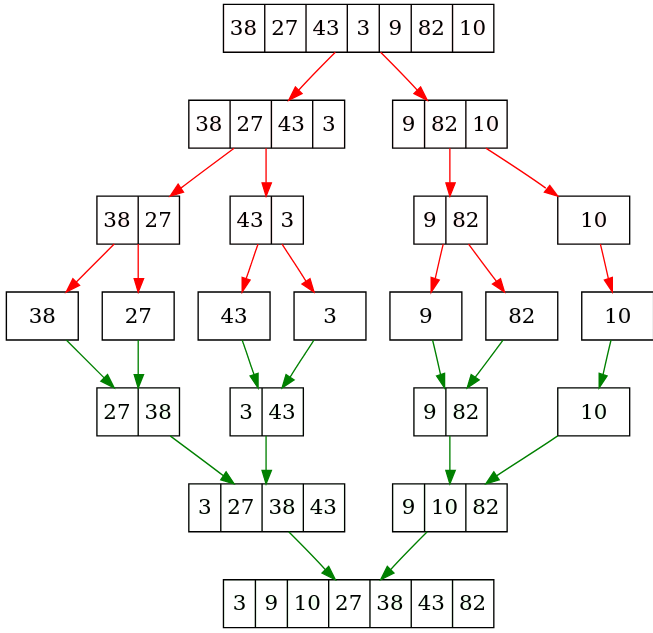
\includegraphics[width=200pt,height=150pt]{slike/mege.png} %merge-sort-example.png}
 	\label{fig:merge-sort}
 	\caption{Sortiranje niza spajanjem pomoću Podijeli-pa-zavladaj paradigme: korak po korak}
 \end{figure}


\begin{example}
	(\textbf{\textit{Množenje cijelih brojeva}}). Poznati algoritam za množenje dva $n$-cifrena broja, koji se uči u osnovnoj školi i zasniva se na množenju cifru po cifru, ima vremensku složenost $O(n^2)$. Konstruisati efikasniji algoritam zasnovan na paradigmi \emph{podijeli pa zavladaj} za problem množenja dva cijela broja.
\end{example}

\begin{solution}
	
	Radi jednostavnosti, bez smanjenja opštosti, pretpostavimo da su ulazni brojevi zapisani u binarnom obliku i da imaju isti broj cifara. Neka su dati brojevi $x$ i $y$, svaki dužine $n$ bitova. Podijelimo ih na lijevu i desnu polovinu: $
	x = x_1 2^{n/2} + x_2,
	\qquad
	y = y_1 2^{n/2} + y_2,
	$ gdje $x_1$, $x_2$, $y_1$ i $y_2$ sadrže $n/2 (\pm 1)$ bitova. 	Tada vrijedi
	
	$
	xy = (x_1 2^{n/2} + x_2)\cdot (y_1 2^{n/2} + y_2) =$ 
	$x_1y_1 2^n
	+
	(x_1y_2 + x_2y_1)2^{n/2}
	+
	x_2y_2.
	$
	
	Na osnovu ove formule potrebno je izračunati četiri proizvoda brojeva dužine $ \approx n/2$: $
	x_1y_1,\quad
	x_1y_2,\quad
	x_2y_1,\quad
	x_2y_2.
	$
	
	Rekurzija složenosti tada ima oblik $T(n)=4T(n/2)+O(n),$ pa prema Master teoremi dobijamo $T(n)=O(n^{\log_2 4})=O(n^2),$	što ne predstavlja poboljšanje u odnosu na klasični algoritam.
	
	Da bismo smanjili broj rekurzivnih množenja, koristimo sljedeću ideju:
	
	\begin{enumerate}
		\item Izračunamo $[
		z_1=x_1y_1]$.
		\item Izračunamo
		\[
		z_2=x_2y_2.
		\]
		\item Izračunamo $
		z_3=(x_1+x_2)(y_1+y_2).$
		
	\end{enumerate}
	
	Tada važi $z_3-z_1-z_2=
	x_1y_2+x_2y_1, $ 	pa se mješoviti član može dobiti bez dodatnih množenja. Prema tome, $xy=z_1 2^n	+	(z_3-z_1-z_2)2^{n/2} + z_2.$
	
	Na ovaj način broj rekurzivnih množenja smanjuje se sa četiri na tri, pa rekurzija postaje $T(n)=3T(n/2)+O(n).$ Primjenom Master teoreme dobijamo $T(n)=O(n^{\log_2 3})
	\approx O(n^{1.585}),$ što je asimptotski brže od klasičnog algoritma množenja (Pogledati Primjer 1.13). Ovaj pristup poznat je kao \textit{Karacubinov algoritam} (eng. {Karatsuba multiplication algorithm}).
\end{solution}

\section{Algoritamska paradigma vraćanja unazad}

{Vraćanje unazad} predstavlja algoritamsku paradigmu zasnovanu na rekurzivnoj izgradnji rješenja korak po korak. Tokom konstrukcije rješenja algoritam u svakom koraku provjerava da li trenutno parcijalno rješenje može biti prošireno u validno konačno rješenje. Ukoliko se utvrdi da neki izbor narušava ograničenja problema ili ne može dovesti do dopustivog rješenja, algoritam odustaje od tog pravca pretrage i vraća se na prethodnu odluku kako bi ispitao druge mogućnosti.

Ova paradigma može se posmatrati kao unaprijeđena verzija pristupa grube sile. Dok algoritmi grube sile ispituju sva moguća rješenja, algoritmi vraćanja unazad nastoje što ranije eliminisati dijelove prostora pretrage za koje se može zaključiti da ne sadrže validno rješenje. Na taj način često se postižu značajne uštede u vremenu izvršavanja.

Osnovna ideja paradigme sastoji se u tome da se rješenje gradi inkrementalno, dodavanjem jedne komponente u svakom koraku. Nakon svakog proširenja parcijalnog rješenja provjerava se da li ono i dalje zadovoljava uslove problema. Ako je odgovor negativan, pretraga se vraća na prethodni korak i pokušava drugačiji izbor.

Paradigma vraćanja unazad posebno je pogodna za probleme kod kojih:

\begin{itemize}
	\item rješenje možemo graditi postepeno;
	\item nakon svakog koraka možemo provjeriti da li je parcijalno rješenje dopustivo;
	\item postoji veliki broj mogućih kombinacija koje treba sistematski istražiti.
\end{itemize}

Tipični primjeri primjene ove paradigme uključuju Problem osam dama, bojenje grafa, sudoku, problem ruksaka, generisanje permutacija i kombinacija sa određenim ograničenjima, te mnoge druge kombinatorne optimizacione probleme. Opšti pseudokod paradigme vraćanja unazad dat je Algoritmom~\ref{alg:backtrack}.

\begin{algorithm}
	\begin{algorithmic}[1]
		\Procedure{Backtrack}{$x$}
		
		\If{$x$ nije dopustivo parcijalno rješenje}
		\State \Return
		\EndIf
		
		\If{$x$ predstavlja potpuno rješenje}
		\State Sačuvaj ili obradi rješenje $x$
		\State \Return
		\EndIf
		
		\For{svaku moguću odluku $e$}
		\State \textsc{Backtrack}(proširi $x$ sa $e$)
		\EndFor
		
		\EndProcedure
	\end{algorithmic}
	\caption{Opšti obrazac paradigme vraćanja unazad.}
	\label{alg:backtrack}
\end{algorithm}

Implementacija ove paradigme prirodno vodi ka konstrukciji \textit{stabla stanja} (eng. \emph{state-space tree}). Svaki čvor stabla predstavlja jedno parcijalno rješenje, dok grane odgovaraju mogućim proširenjima tog rješenja. Rekurzivni pozivi algoritma odgovaraju obilasku ovog stabla. Kada se utvrdi da određena grana ne dovodi do validnog rješenja, dalji obilazak te grane se prekida, čime se izbjegava nepotrebno pretraživanje.

U najgorem slučaju algoritmi vraćanja unazad i dalje mogu imati eksponencijalnu vremensku složenost, jer je ponekad potrebno istražiti veoma veliki broj mogućih kombinacija. Ipak, zahvaljujući ranom odbacivanju nedopustivih parcijalnih rješenja, oni su u praksi često znatno efikasniji od pristupa grube sile.

    %https://www.programiz.com/dsa/backtracking-algorithm ==> primjer 1...
    
 \begin{example}
 	(\textbf{\emph{Problem $N$ kraljica}}). Neka je data šahovska ploča dimenzija $N \times N$. Postaviti $N$ kraljica na ploču tako da se nikoje dvije kraljice međusobno ne napadaju. Riješiti problem primjenom paradigme vraćanja unazad.
 \end{example}
 
 \begin{solution}
 	
 	Posmatrajmo najpoznatiju varijantu ovog problema, problem osam kraljica ($N=8$). Jedno dopustivo rješenje prikazano je na Slici~\ref{fig:8-queen-sol-example}.
 	
 	\begin{figure}[H]
 		\centering
 		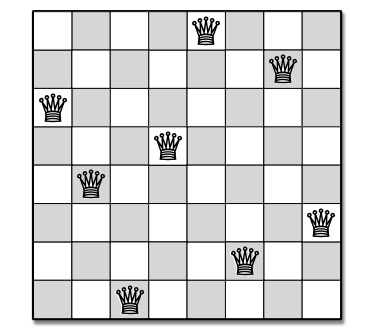
\includegraphics[width=200pt,height=180pt]{slike/n-queen-problem.png}
 		\caption{Primjer jednog rješenja problema osam kraljica.}
 		\label{fig:8-queen-sol-example}
 	\end{figure}
 	
 	Pošto se dvije kraljice ne smiju nalaziti u istom redu, svako rješenje možemo predstaviti nizom dužine $N$. Element na poziciji $i$ označava kolonu u kojoj je postavljena kraljica u $i$-tom redu šahovske ploče. Na primjer, raspored kraljica prikazan na Slici~\ref{fig:8-queen-sol-example} može se predstaviti nizom $
 	[5, 7, 1, 4, 2, 8, 6, 3]. $	Vrijednost na svakoj poziciji određuje kolonu u kojoj se smiješta kraljica u odgovarajući red.
 	
 	Algoritam vraćanja unazad započinje od praznog rješenja. U svakom koraku pokušava se postaviti nova kraljica u naredni red šahovske ploče. Drugim riječima, parcijalno rješenje se proširuje dodavanjem jedne nove komponente, odnosno izborom kolone u kojoj će se nalaziti kraljica u trenutno obrađivanom redu. Nakon svakog dodavanja provjerava se da li novopostavljena kraljica napada neku od prethodno postavljenih kraljica. Konflikt postoji ukoliko se dvije kraljice nalaze:
 	
 	\begin{itemize}
 		\item u istoj koloni;
 		\item na istoj glavnoj dijagonali;
 		\item na istoj sporednoj dijagonali.
 	\end{itemize}
 	
 	Ako se utvrdi postojanje konflikta, trenutno parcijalno rješenje ne može biti dio nijednog dopustivog konačnog rješenja. U tom slučaju algoritam odbacuje posljednji izbor, vraća se na prethodni nivo pretrage i pokušava postaviti kraljicu u neku drugu kolonu istog reda.
 	
 	Proces se nastavlja sve dok:
 	
 	\begin{itemize}
 		\item ne bude konstruisano dopustivo rješenje dužine $N$, čime su kraljice uspješno postavljene u sve redove šahovske ploče; ili
 		\item ne budu iscrpljene sve mogućnosti pretrage, kada zaključujemo da rješenje ne postoji.
 	\end{itemize}
 	
 	Problem $N$ kraljica predstavlja jedan od najpoznatijih primjera primjene paradigme vraćanja unazad, jer omogućava veoma efikasno odbacivanje velikog broja parcijalnih rješenja koja ne mogu dovesti do validnog rasporeda kraljica.
 \end{solution}
 
   
Implementacija problema je data narednim k\^odom. 

\begin{minted}[fontsize=\footnotesize,scale=0.8]{python}
	
   def NQueens(niz, N):
       if len(niz) == N: # kompletno rješenje
               return niz
       else:
              for col in range(N):
                  kandidat = niz + [col]
                  if valid(kandidat):
                      rezultat = NQueens(kandidat, N)
                      if rezultat is not None:
                          return rezultat
              return None

#main
N = 8
sol = NQueens([], N)       
if sol != None:
   print("Rješenje je: ", sol)
else:
   print("Nema rješenja") #npr. za N=3
   
\end{minted}
%%https://codeahoy.com/learn/recursion/ch10/
\begin{figure}
	\centering
	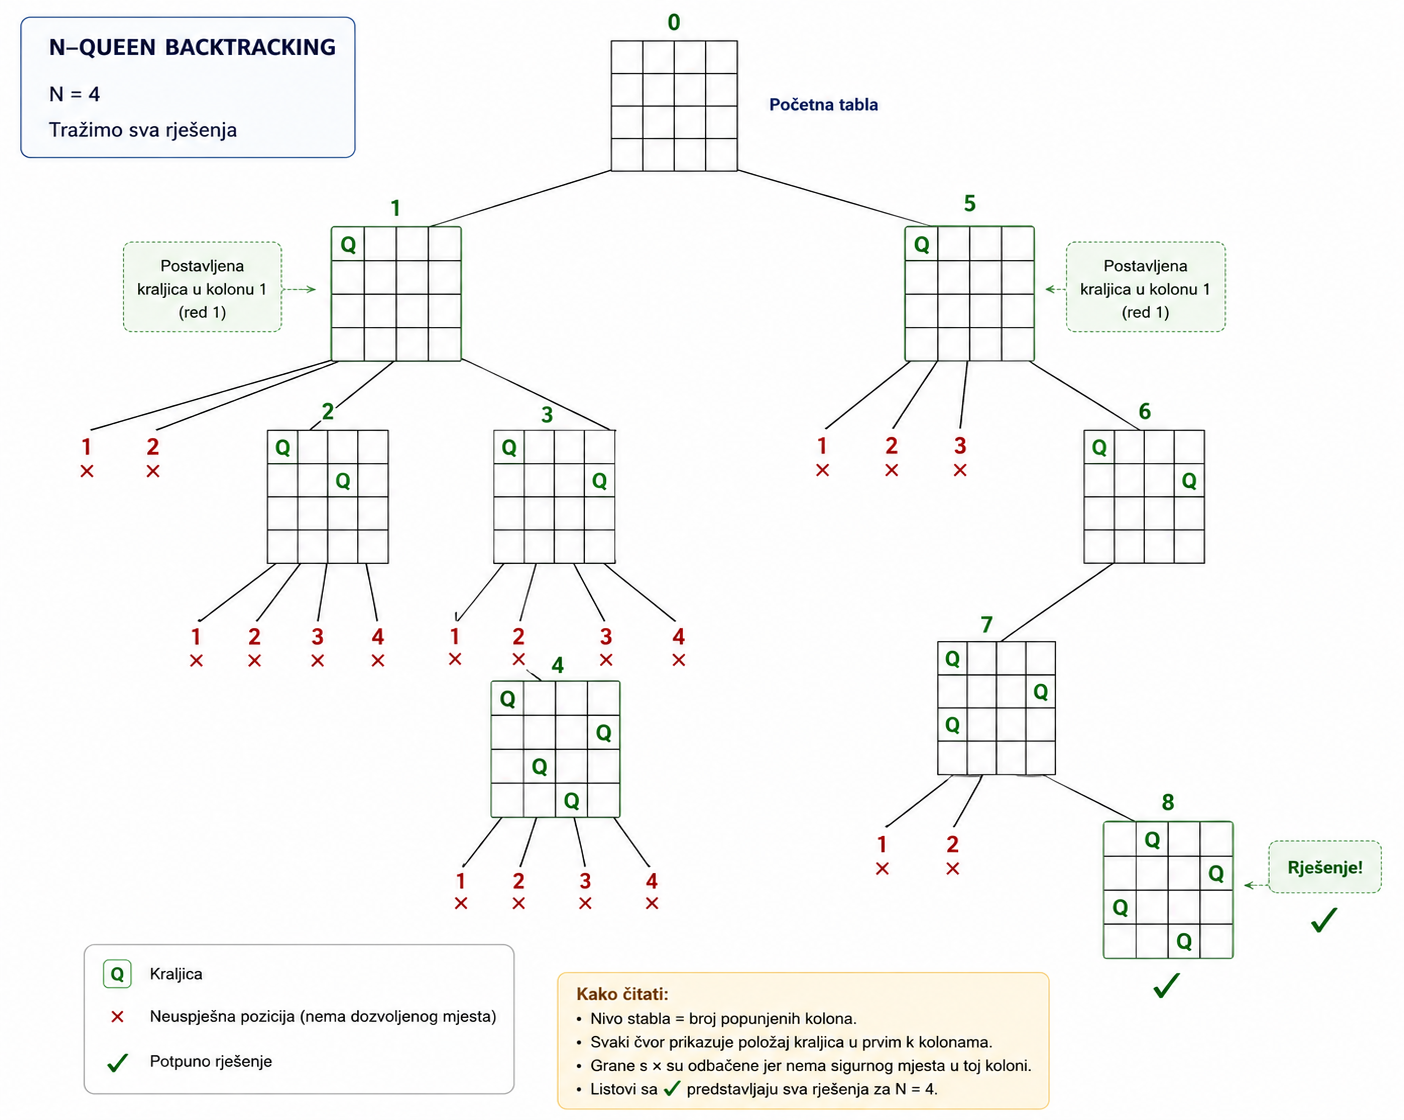
\includegraphics[width=350pt, height=280pt]{slike/n-queen-backtracking.png} %recursion-tree-backtracking-n-queens-1.png}
	\caption{Primjer stabla stanja formiranog algoritmom vraćanja unazad za problem 4 kraljice.}
\end{figure}
%\protect\footnotemark\footnotetext{Slika sa linka \url{https://towardsdatascience.com/genetic-algorithm-vs-backtracking-n-queen-problem-cdf38e15d73f}}

Napomenimo da ovdje nismo prikazali implementaciju funkcije \texttt{valid}(), koja vraća \textit{True} ako su pozicije kraljica  validne, u protivnom vraća \textit{False}. Ovo ostavljamo čitaocu kao zadatak za vježbanje. 


\end{solution}


    
 % Što se tiče problema koje ova paradigma rješava, dijelimo ih na tri tipa:
  %\begin{itemize}
  %	\item   \textit{Problem odlučivanja} -- U ovom slučaju tražimo izvodljivo rješenje.
  %	\item   \textit{Problem optimizacije} – U ovome tražimo najbolje rješenje.
  %	\item   \textit{Problem enumeracije} – U ovome nalazimo sva izvodljiva rješenja.
  %\end{itemize}


%https://codeahoy.com/learn/recursion/ch11/: THE SUM OF 4 SQUARES:

\begin{example}
	(\textbf{Problem sume 4 kvadrata}). Lagranžova teorema o 4 kvadrata kaže da se svaki prirodni broj može napisati kao zbir četiri broja koji su kvadrati nekih brojeva. Neka je dat broj $n$. Naći četiri kvadratna broja koji u zbiru daju broj $n$ pomoću algoritma vraćanja unazad.	Npr. za $n=2000$, vrijedi $1764 + 196 + 36 + 4 = 2000. $
\end{example}

\begin{solution}
	Rješenje problema predstavlja četvorka $sol = (a, b, c, d)$ prirodnih brojeva, tako da vrijedi $a^2 + b^2 + c^2 + d^2 = n$. Ideja rekurzije je odabrati svaki  od brojeva jedan po jedan, dok ne nađemo četvorku koja odgovara uslovima zadatka. Svaki put kada dodamo novi broj $x$ u rješenje \emph{sol}, naredni rekurzivni poziv ispituje trenutno zbir kvadrata brojeva u proširenom rješenju \emph{sol}. Ako vrijednost prelazi $n$, algoritam vrši vraćanje unazad i bira novog kandidata za proširivanje rješenja. 
	
 Implementacija algoritma vraćanja unazad za ovaj problem je dat narednim k\^odom.
 
 \begin{minted}[fontsize=\footnotesize,scale=0.8]{python}
from math import sqrt, pow

def FourSquareSum(sol):
	sum = 0
	for s in sol:
		sum += pow(s, 2)
	return sum

  def FourSumSquares(sol, n):
	if len(sol) == 4:
		if FourSquareSum(sol) == n:
			print(sol)
			return 
	else:
		for i in range(1, int(sqrt(n))+2):
			solI = sol + [i]
			sum_sol_i = FourSquareSum(solI)
			if sum_sol_i <= n-(4-len(solI)): # else backtrack  
				FourSumSquares(solI, n) 
  # poziv metode
  FourSumSquares([], 20)
 \end{minted}
	
	Kao što primijećujemo u prethodnom kodu, ako je \emph{sol} kardinalnosti 4, i ako je zbir kvadrata njegovih elemenata jednak $n$, ispisujemo \emph{sol} kao rješenje. U protivnom, ako je $|sol|<4$, (parcijalno) rješenje \emph{sol} proširujemo ubacujući naredni broj (varijabla $i\in \{1, \ldots, \lfloor\sqrt{n} \rfloor + 1 \}$), dobijajući niz \emph{solI}.  Ako je zbir kvadrata elemenata iz \emph{sol} veći od $n-(4 - |solI|)$, ovakva ekstenzija nikada neće voditi ka rješenju koje zadovoljava uslove zadatka, pa pretraga ide unazad, rekurzivno,  ispitujući druge kandidate za proširenje trenutnog rješenja \emph{sol}. Inicijalno, rješenje \emph{sol} je predstavljeno praznim nizom.
	 
\end{solution}
 
 
\section{Pohlepni algoritmi}

\textit{Pohlepni algoritmi}  predstavljaju algoritamsku paradigmu u kojoj se u svakom koraku donosi lokalno najbolja odluka o proširenju parcijalnog rješenja prema unaprijed definisanom kriterijumu. Osnovna ideja je da se problem rješava nizom lokalno optimalnih izbora, uz pretpostavku da će takvi izbori dovesti do kvalitetnog, a ponekad i optimalnog globalnog rješenja.

Za razliku od algoritama vraćanja unazad ili dinamičkog programiranja, pohlepni algoritmi ne preispituju ranije donesene odluke. Jednom kada se neka komponenta uključi u rješenje, ona se više ne uklanja niti mijenja. Zbog toga su pohlepni algoritmi obično veoma efikasni, ali ne garantuju uvijek pronalazak optimalnog rješenja.

Drugim riječima, algoritam u svakom koraku bira opciju koja je trenutno najpovoljnija, bez razmatranja mogućih posljedica tog izbora na buduće korake. Zbog toga, uspješnost ovog pristupa zavisi od strukture problema. Za određene klase problema može se dokazati da lokalno optimalni izbori vode ka globalno optimalnom rješenju, dok kod drugih problema pohlepni pristup daje samo aproksimativna/heuristička rješenja. 

U neformalnom smislu, pohlepni algoritam započinje od praznog ili djelimično izgrađenog rješenja i zatim ga iterativno proširuje komponentama koje imaju najveću trenutnu korist. Proces se nastavlja sve dok se ne dobije potpuno rješenje ili dok se ne iscrpe sve mogućnosti za dopustivo proširenje.

Opšta shema pohlepnog pristupa prikazana je Algoritmom~\ref{alg:greedy-algorithm}. Ulaz u algoritam čine instanca problema $\mathcal{P}$ i pohlepna funkcija $g$, koja procjenjuje kvalitet mogućih proširenja trenutnog rješenja.

U svakoj iteraciji izvršavaju se sljedeći koraci:

\begin{itemize}
	\item određuje se skup svih komponenti koje na dopustiv način mogu proširiti trenutno parcijalno rješenje;
	\item među njima se bira komponenta sa najboljom vrijednošću pohlepne funkcije;
	\item izabrana komponenta se dodaje trenutnom rješenju.
\end{itemize}

Proces se ponavlja sve dok postoji barem jedna komponenta koja može dopustivo proširiti trenutno rješenje. Nakon toga algoritam vraća konstruisano rješenje.

\begin{algorithm}
	\begin{algorithmic}[1]
		\State \textbf{Ulaz:} instanca problema, pohlepna funkcija $g$
		\State \textbf{Izlaz:} (aproksimativno) rješenje problema
		\State $x \gets$ inicijalno parcijalno rješenje
		\State $\mathcal{C} \gets$ skup dopustivih proširenja rješenja $x$
		
		\While{$\mathcal{C} \neq \emptyset$}
		\State $e \gets$ lokalno najbolja komponenta iz $\mathcal{C}$ shodno vrijednosti funkc. $g$
		\State $x \gets$ proširi rješenje $x$ komponentom $e$
		\State $\mathcal{C} \gets$ odredi nova dopustiva proširenja rješenja $x$
		\EndWhile
		
		\State \Return $x$
	\end{algorithmic}
	\caption{Opšta shema pohlepnog algoritma.}
	\label{alg:greedy-algorithm}
\end{algorithm}

Da bi se neki problem mogao rješavati pohlepnim pristupom, potrebno je definisati:

\begin{enumerate}
	\item skup komponenti od kojih se gradi rješenje;
	\item reprezentaciju parcijalnog rješenja;
	\item kriterijum za izbor sljedeće komponente, odnosno pohlepnu funkciju;
	\item uslove dopustivosti proširenja parcijalnog rješenja.
\end{enumerate}

Najpoznatiji primjeri primjene pohlepnih algoritama uključuju problem izbora aktivnosti, konstrukciju Hafmanovog stabla, algoritme za pronalaženje minimalnog razapinjućeg stabla (Kruskalov i Primov algoritam), te određene varijante problema najkraćih puteva, kao što je Dijkstrin algoritam za grafove sa nenegativnim težinama grana.

Glavna prednost pohlepnih algoritama jeste njihova jednostavnost implementacije i mala vremenska složenost. Međutim, njihov osnovni nedostatak je što lokalno najbolji izbor ne mora uvijek voditi globalno optimalnom rješenju. Zbog toga je prije primjene ove paradigme potrebno dokazati da problem posjeduje tzv. \emph{pohlepno svojstvo} (eng. \emph{greedy-choice property}), odnosno da optimalno rješenje može biti izgrađeno nizom lokalno optimalnih odluka.


Ovu paradigmu koristimo kada je potrebno pronaći rješenje zadovoljavajućeg kvaliteta u relativno kratkom vremenu, uz jednostavnu implementaciju algoritma. Zbog svoje efikasnosti i konceptualne jednostavnosti, pohlepni pristup često predstavlja prvi korak u rješavanju složenih kombinatornih i optimizacionih problema.

Pohlepni algoritmi se takođe često koriste za generisanje početnih rješenja koja se kasnije dodatno poboljšavaju naprednijim metodama, kao što su lokalna pretraga, metaheuristike ili egzaktni algoritmi. U tom smislu, oni pružaju korisnu polaznu osnovu za razumijevanje strukture problema i procjenu kvaliteta rješenja koja se mogu dobiti korištenjem jednostavnih konstruktivnih heuristika.

U nastavku prikazujemo nekoliko primjera primjene pohlepnih algoritama na različite kombinatorne probleme.

\begin{example}
	(\textbf{\emph{Problem razmjenjivanja novca}}).
	
	Neka je dato $X$ KM i skup apoena $x_1, x_2, \ldots, x_k$, pri čemu je svaki apoen dostupan u neograničenoj količini. Pretpostavimo da su $X$ i svi apoeni prirodni brojevi. \\
	
	
	Na koji način razmijeniti iznos $X$ tako da ukupan broj novčanica i kovanica bude minimalan? Problem riješiti primjenom pohlepnog pristupa.
\end{example}

\begin{solution}
	
	Definišimo najprije strukturu rješenja. Svako rješenje može se predstaviti $k$-torkom $(p_1,p_2,\ldots,p_k),$ gdje $p_i$ označava broj iskorištenih apoena vrijednosti $x_i$. Rješenje je dopustivo ukoliko vrijedi $\sum_{i=1}^{k} p_i x_i = X.$
	
	Parcijalno rješenje predstavlja djelimično formiranu kombinaciju apoena $(p_1,p_2,\ldots,p_s), s \leq k,$ za koju vrijedi $\sum_{i=1}^{s} p_i x_i \leq X.$ 	Takvo rješenje se može dalje proširivati dodavanjem novih apoena.
	
	Osnovna ideja pohlepnog algoritma jeste da se u svakom koraku bira najveći apoen koji ne premašuje preostali iznos koji treba razmijeniti. Nakon izbora apoena uzima se maksimalan mogući broj novčanica ili kovanica tog apoena, a zatim se isti postupak ponavlja za preostali iznos.\\ 
	
	Pretpostavimo da su apoeni sortirani opadajuće: $ x_1 > x_2 > \cdots > x_k.$
	
	Neka je $X' = X - \sum_{j=1}^{s} p_j x_j$ preostali iznos koji još treba razmijeniti. Tada se bira najveći apoen $x_i$ za koji važi $x_i \leq X',$ a broj njegovih pojavljivanja određuje se kao $p_i=\left\lfloor \frac{X'}{x_i}\right\rfloor.$  	Na taj način parcijalno rješenje se proširuje novom komponentom, nakon čega se ažurira vrijednost preostalog iznosa. Postupak se ponavlja sve dok preostali iznos ne postane nula.
	
	%Za standardne novčane sisteme (npr. konvertibilna marka, euro ili američki dolar) ovakav pohlepni postupak daje optimalno rješenje, odnosno minimalan broj novčanica i kovanica. Međutim, za proizvoljno definisane skupove apoena to ne mora uvijek biti slučaj, pa je u takvim situacijama potrebno koristiti naprednije algoritamske tehnike.
\end{solution}

Implementacija algoritma ovog problema  je data u nastavku.
	 \begin{minted}[fontsize=\footnotesize,scale=0.75]{python}
	 def razmijeni(P, X):
	 	rjesenje = []
	 	i = 0
	 	usitnjeno, brojNovcanica = 0, 0
	 	sortApoeni = sorted(P) # sort apoene opadajuće
	 	while i <  n and usitnjeno < X :
	 		pi = (X - usitnjeno) // P[i]  #br. novcanica sortApoeni[i]
	 		if pi > 0:
	 			usitnjeno = usitnjeno + pi * sortApoeni[i]
	 			brojNovcanica = brojNovcanica + pi
	 		i = i + 1
	 	if usitnjeno == X:
	 		return brojNovcanica
	 	else:
	 		return -1 # ne može se usitniti
	 \end{minted} 
\end{solution}

\textbf{Vremenska složenost}. Sortiranje algoritma zahtijeva $O(n \log n)$ vreme\-na. Dalje, glavna petlja se izvršava u $O(n)$ vremenu, odakle slijedi da je ukupno vrijeme izvršavanja algoritma jednako $O(n \log n)$, što je, svakako, polinomi\-jalno. Za kanonske sisteme apoena, kakvi se koriste u većini standardnih valuta, pohlepni algoritam daje optimalno rješenje.   %Napomenimo da ovakvom strategijom garantujemo nalazak optimalnog rje\-šenja problema, (ili utvrđujemo da rješenje ne postoji) što se formalno može i pokazati. 


\begin{example}
	(\textbf{\emph{Razlomljeni problem ruksaka}}). Ovaj problem predstavlja relaksiranu verziju klasičnog problema ruksaka. Za razliku od standardne varijante, gdje se svaki proizvod mora uzeti u cijelosti ili se uopšte ne uzima, ovdje je dozvoljeno uzeti proizvoljan dio proizvoda. Takva pretpostavka ima smisla za proizvode koji se mogu dijeliti, kao što su šećer, brašno, ulje ili gorivo. \\
	
	Dat je skup proizvoda, pri čemu svaki proizvod $i$ ima težinu $w_i$ i vrijednost $p_i$, kao i ruksak kapaciteta $C$. Potrebno je odrediti koje proizvode, odnosno koje njihove dijelove, treba smjestiti u ruksak tako da ukupna vrijednost bude maksimalna, uz poštovanje ograničenja kapaciteta.
	
	Problem riješiti primjenom pohlepnog pristupa.
\end{example}

\begin{solution}
	
	Posmatrajmo instancu problema $n=3,
	w=[10,20,30],
	p=[60,100,120],$ 	pri čemu je kapacitet ruksaka jednak $C=50$.
	
	Optimalno rješenje dobija se tako što se prvi i drugi proizvod uzimaju u potpunosti, dok se od trećeg proizvoda uzima samo dio. Ukupna težina prva dva proizvoda iznosi $10+20=30$, pa u ruksaku ostaje još $20$ jedinica slobodnog prostora. Kako treći proizvod ima težinu $30$, moguće je uzeti samo njegov dio $\frac{20}{30}=\frac{2}{3}.$  Ukupna vrijednost ruksaka tada iznosi 	$60 + 100 + \frac{2}{3}\cdot 120 = 240.$ \\
	\medskip
	\textit{Struktura rješenja.}	Rješenje predstavljamo vektorom $c=(c_1,c_2,\ldots,c_n),$ gdje je $0\leq c_i\leq 1$ udio proizvoda $i$ koji se nalazi u ruksaku. Pri tome mora važiti ograničenje kapaciteta $	\sum_{i=1}^{n} c_i w_i \leq C.$
	
	\medskip
	
	\textit{Parcijalna rješenja i komponente rješenja.}
	Parcijalno rješenje čini bilo koji skup već odabranih proizvoda i njihovih udjela koji ne narušavaju kapacitet ruksaka. Komponente rješenja predstavljaju proizvodi koji još nisu razmatrani i koji mogu dopustivo proširiti trenutno rješenje.
	
	\medskip
	
	\textit{Pohlepna funkcija.}
	Ključna ideja je da prednost dajemo proizvodima koji ostvaruju najveću vrijednost po jedinici težine. Za svaki proizvod računamo omjer $
	\rho_i=\frac{p_i}{w_i}.$  Vrijednost $\rho_i$ predstavlja profit ostvaren po jedinici zauzetog kapaciteta i prirodno određuje prioritet proizvoda. Najprije se sortiraju proizvode opadajuće prema vrijednosti $\rho_i$. Neka je nakon sortiranja redoslijed proizvoda označen indeksima $1,2,\ldots,n.$
	
	Algoritam zatim prolazi kroz proizvode tim redoslijedom. Za svaki proizvod uzima se najveći mogući dio koji još može stati u preostali kapacitet ruksaka. Ako proizvod može stati u cijelosti, postavlja se $c_i=1$. U suprotnom, uzima se upravo onaj dio koji popunjava preostali kapacitet: $c_i=  \frac{\text{preostali\_kapacitet}}{w_i}.$  Nakon toga je ruksak popunjen i algoritam se završava.
	
	\medskip
	
	Pohlepni algoritam za razlomljeni problem ruksaka ima vremensku složenost $O(n\log n)$, koja potiče od sortiranja proizvoda (prema omjeru $\frac{p_i}{w_i}$). Za razliku od klasičnog problema ruksaka, kod ove relaksirane varijante može se dokazati da opisani pohlepni pristup uvijek daje optimalno rješenje.
\end{solution}


  Implementacija algoritma je data naredim k\^odom. 
   
   \begin{minted}[fontsize=\footnotesize,scale=0.8]{python}
  def fraction(i):
  	return P[i]/ W[i]
  
  def fraction_knapsack():
  
  	products = [i for i in range(len(W))] #lsit of prods
  	products.sort(key = fraction, reverse=True)
  	#print(products)
  	current_C = C
  	sol, parts = [], []

  	for i in products:
  
  		part = min(current_C / W[i], 1)
  		if part > 0:
  			sol.append(i)
  			parts.append(part)
  			current_C -= part * W[i]
  
  		else: # knapsack filled
  			return sol, parts
          return sol, parts
    #instanca: 
    W = [10, 20, 30]
    P = [60, 100, 120]
    C = 50
    sol, parts = fraction_knapsack()
    print(sol, " parts: ", parts)
  
   \end{minted}

\textit{Kompleksnost algoritma}.  Najviše vremena je utrošeno na sortiranje proi\-zvoda, što iznosi $O(n \log n)$ vremena. Dalje, u glavnoj petlji, koja se vrti najviše $n$ puta,  svaka iteracija se izvršava u konstantnom vremenu. Dakle, vrijeme izvršavanja petlje je $O(n)$. Prema tome, algoritam se izvršava u $O(n \log n)$ vremenu. %Napomenimo da ovaj algoritam takođe garantuje nalazak optimalnog rješenja, što se formalno može i pokazati. 
\end{solution}


\begin{example}
	(\textbf{\emph{Problem pokrivanja skupa}}). 	Neka je dat konačan skup $X$ i familija njegovih podskupova
	$\mathcal{F}\subseteq P(X)$, pri čemu važi 	$\bigcup_{F\in \mathcal{F}} F = X.$ Potrebno je pronaći podfamiliju $S\subseteq \mathcal{F}$ minimalne kardinalnosti takvu da vrijedi $\bigcup_{A\in S} A = X.$ \\
	
	Drugim riječima, cilj je odabrati što manji broj skupova iz familije $\mathcal{F}$ tako da njihova unija pokrije sve elemente skupa $X$. Problem riješiti primjenom pohlepnog pristupa.
\end{example}

\begin{solution}
	
	Posmatrajmo instancu $
	X=\{1,2,3,4,5\},$ i familiju skupova  $
	\mathcal{F}=
	\big\{
		\{1,2,3\},
		\{1,4\},
		\{2,4,5\},
		\{2,3\},
		\{4,5\},
		\{1,5\}
		\big\}.$
	
	Jedno optimalno rješenje je $S= \big\{
		\{1,2,3\},
		\{2,4,5\}
		\big\},$	jer unija skupova u rješenju pokriva čitav skup $X$, a pri tome je $|S|=2.$
	
	Problem pokrivanja skupa ima brojne praktične primjene. Na primjer, može predstavljati zadatak izbora minimalnog broja stručnjaka u komisiji tako da svaka potrebna oblast bude zastupljena barem jednim članom komisije. Slične primjene javljaju se u planiranju mreža senzora, raspoređivanju resursa i izboru lokacija za pružanje usluga.
	
	\medskip
	
	\textit{Struktura rješenja.}	Rješenje problema je predstavljeno podfamilijom skupova $S\subseteq \mathcal{F}$	takva da njihova unija pokriva sve elemente skupa $X$.
	
	\medskip
	
	\textit{Parcijalna rješenja i komponente rješenja.}
	Parcijalno rješenje predstavlja proizvoljna podfamilija
    $S\subseteq \mathcal{F},$  	koja ne mora nužno pokrivati čitav skup $X$.  Komponente koje mogu proširiti trenutno rješenje jesu svi skupovi iz familije $\mathcal{F}\setminus S.$ Proširenje parcijalnog rješenja vrši se dodavanjem novog skupa: $
	  S' = S \cup {C}, C\in \mathcal{F}\setminus S.$
	
	\medskip
	
	\textit{Pohlepna funkcija.}	Neka trenutno parcijalno rješenje $S$ pokriva skup elemenata $ X_S= \bigcup_{A\in S} A.$	Preostali nepokriveni elementi dati su skupom $
	X\setminus X_S.
	$   Intuitivno, najbolji izbor u datom koraku jeste skup koji pokriva najveći broj trenutno nepokrivenih elemenata. Zbog toga definišemo pohlepnu funkciju 	$$ g(S,C)= \left| C\cap (X\setminus X_S) \right|,$$
 koja mjeri broj novih elemenata koje skup $C$ doprinosi trenutnom rješenju.	U svakoj iteraciji bira se skup $ C^* = \arg\max_{C\in \mathcal{F}\setminus S}
	g(S,C),
	$ odnosno skup koji pokriva najveći broj još nepokrivenih elemenata.
	
	\medskip
	
	Pohlepni algoritam započinje praznim rješenjem $S=\emptyset$. U svakoj iteraciji bira skup $C^*$ koji maksimizuje funkciju $g$, dodaje ga u rješenje i ažurira skup pokrivenih elemenata. Postupak se ponavlja sve dok svi elementi skupa $X$ ne budu pokriveni ili ne postoji više skupova koji se mogu dodati u rješenje.  Važno je naglasiti da opisani pohlepni algoritam ne garantuje uvijek optimalno rješenje. Ipak, zbog svoje jednostavnosti i efikasnosti veoma je često korišten u praksi i predstavlja jednu od najpoznatijih aproksimativnih metoda za problem pokrivanja skupa.
	
	Radi efikasnije implementacije, umjesto samih skupova u rješenju se čuvaju odgovarajući indeksi unutar familije $\mathcal{F}$.
\end{solution}

Implementacija algoritma  je data u nastavku sljedećim k\^odom.

\begin{minted}[fontsize=\footnotesize,scale=0.8]{python}
	def g(X_S, C):
		return len((X.difference(X_S)).intersection(C))
	
	def cover_X():
		X_S = set(())
		S = [] # solution
	
		while(X_S != X):
			C_star = istar = None
			g_best = 0
	
			for i in range(len(F)):# iteration best-next
				if i  not  in S: 
					g_i = g(X_S, F[i])
					if g_best < g_i:
						g_best = g_i
						i_star = i
			X_S = X_S.union(F[i_star]) #update cover
			S.append(i_star)
		return  S            
	
	#instanca: 
	X = {1, 2, 3, 4, 5}
	F = [{1, 2, 3}, {1, 4}, {2, 4, 5}, {2, 3}, {4, 5}, {1, 5}]
	sol = []
	C = 50
	sol = cover_X()
	print(sol)
	
\end{minted}

\textit{Vremenska složenost}. Glavna \texttt{while}-petlja izvršava najviše $n$ iteracija. U unutrašnjoj \texttt{for}-petlji, koja se izvršava  $ |\mathcal{F}|$ puta, najskuplja operacija je poziv pohlepne funkcije \textit{g}, koja se izvršava u linearnom vremenu, tj. u $O(n)$. Dakle, kompleksnost čitave \texttt{for} petlje je $O(n \cdot  |\mathcal{F} |)$. Zajedno, kompleksnost algoritma je $O(n^2 \cdot  |\mathcal{F} |)$. Na osnovu dobijenog, zaključujemo da efikasnost algoritma najviše zavisi od veličine skupa $\mathcal{F}$. 

Napomenimo da ovako dizajniran algoritam ne garantuje nalazak opti\-malnog rješenja  kao u prethodna dva problema. Uzmimo npr. instancu $X= \{1, 2, 3, 4, 5, 6\}$, te $$\mathcal{F}= \{\{1,2\}, \{3, 4\}, \{4, 5\}, \{3, 6\}, \{5\}, \{6\} \}.$$   
  Prva iteracija u algoritmu će odabrati, prvi skup $\{1, 2\}$ i dodati ga u parcijalno rješenje. Naredna iteracija odabire skup $\{3, 4\}$. Nakon toga, bira se $\{4, 5\}$, pa $\{6\}$. Dakle, dobijeno rješenje je kardinalnosti 4. Međutim, ono očigledno ne predstavlja optimalno rječenje. 
  
  Optimalno rješenje je veličine 3 i dato je sa $\{ \{1, 2\}, \{3, 6\}, \{4,5\}\}$.  
	 
\end{solution}

\begin{example}
	(\textbf{\emph{Problem sekvencijalnog raspoređivanja poslova}}).
	
	Dat je skup poslova, pri čemu je za svaki posao poznat krajnji rok izvršavanja (eng. \emph{deadline}) i profit koji se ostvaruje ukoliko posao bude završen najkasnije do tog roka. Pretpostavimo da je za izvršavanje svakog posla potrebno tačno jedna jedinica vremena, te da svi poslovi mogu započeti od trenutka $t=0$.\\ 

	
	Potrebno je odabrati podskup poslova i odrediti njihov raspored izvršavanja tako da ukupan ostvareni profit bude maksimalan. Pri tome vrijedi ograničenje da se u svakoj jedinici vremena može izvršavati najviše jedan posao.	Problem riješiti primjenom paradigme pohlepnih algoritama.
\end{example}

\begin{solution}
	
	Posmatrajmo sljedeću instancu problema.
	
	\begin{center}
		\begin{tabular}{ccc}
			\emph{Posao} & \emph{Krajnji rok} & \emph{Profit} \\ \hline \hline 
			1 & 4 & 20 \\
			2 & 1 & 10 \\
			3 & 1 & 40 \\
			4 & 1 & 30 \\ \hline
		\end{tabular}
	\end{center}
	
	Optimalno rješenje u ovom slučaju čine poslovi $\{3,1\}$, čiji je ukupan profit jednak $40 + 20 = 60.$
	
	Posmatrajmo sada drugu instancu problema.
	
	\begin{center}
		\begin{tabular}{ccc}
			\emph{Posao} & \emph{Krajnji rok} & \emph{Profit} \\  \hline \hline
			1 & 2 & 100 \\
			2 & 1 & 19 \\
			3 & 2 & 27 \\
			4 & 1 & 25 \\
			5 & 3 & 15 \\ \hline
		\end{tabular}
	\end{center}
	
	Jedno optimalno rješenje dobija se izvršavanjem poslova $\{3,1,5\}$. Poslovi se mogu rasporediti u vremenske intervale tako da poštuju zadate rokove, pri čemu je ukupan profit $27 + 100 + 15 = 142.$
	
	\medskip
	
	Prva ideja za rješavanje ovog problema bila bi potpuna enumeracija svih podskupova poslova. Za svaki generisani podskup provjerila bi se dopustivost rasporeda i izračunao ostvareni profit. Međutim, broj mogućih podskupova jednak je $2^n$, pa takav pristup postaje neupotrebljiv već za umjerene vrijednosti $n$.
	
	Zbog toga razmatramo pohlepni pristup.
	
	\medskip
	
	\textit{Struktura rješenja.} Rješenje problema predstavlja skup odabranih poslova zajedno sa njihovim rasporedom izvršavanja. Rješenje je dopustivo ako:
	
	\begin{itemize}
		\item svaki odabrani posao bude završen najkasnije do svog krajnjeg roka;
		\item u svakom vremenskom trenutku bude izvršavan najviše jedan posao.
	\end{itemize}
	
	\medskip
	
	\textit{Parcijalno rješenje i njegovo proširenje.}
	Parcijalno rješenje predstavlja bilo koji dopustiv raspored dijela poslova. Komponente koje mogu proširiti parcijalno rješenje jesu poslovi koji još nisu raspoređeni, a koji se mogu dodati bez narušavanja ograničenja problema. 	Proširenje parcijalnog rješenja podrazumijeva dodavanje novog posla u neki slobodan vremenski interval tako da njegov krajnji rok ostane zadovoljen. Recimo, slobodan vremenski interval bi mogao biti onaj koji je najkasniji mogući a ne narušava ni krajnji rok izvršavanja konkretnog posla, niti postoji konflikt između poslova koji bi se simultano izvršavali u istom vremenskom intervalu. 
	
	\medskip
	
	\textit{Pohlepna funkcija.}
	Intuitivno je razumno dati prednost poslovima koji donose veći profit. Zbog toga se poslovi najprije sortiraju po profitu u opadajućem poretku.\\
	
	Neka je trenutno parcijalno rješenje označeno sa $I_s$. U svakoj iteraciji bira se neraspoređeni posao sa najvećim profitom. Ukoliko je moguće pronaći  slobodan vremenski interval prije krajnjeg roka, posao se dodaje u raspored. U suprotnom, posao se odbacuje i razmatra se naredni posao iz sortirane liste.  Da bi se ostavilo što više prostora za buduće poslove, odabrani posao se smiješta u \textit{posljednji} (najkasniji) slobodan vremenski interval koji ne prelazi njegov krajnji rok.
	
	\medskip
	
	Algoritam se može opisati sljedećim koracima:
	
	\begin{enumerate}
		\item Sortirati poslove po profitu u opadajućem poretku.
		\item Poštujući redoslijed sortiranja, idući od posla do posla, pronaći  (najkasniji) slobodan vremenski interval prije krajnjeg roka.
		\item Ako takav interval postoji, posao rasporediti u njega.
		\item U suprotnom, posao odbaciti i preći na drugi.
		\item Nakon razmatranja svih poslova vratiti dobijeni raspored.
	\end{enumerate}
	
	Pohlepni algoritam za ovaj problem izvršava se znatno brže od potpune enumeracije, a pritom daje optimalno rješenje. Ključna ideja sastoji se u tome da se najprofitabilniji poslovi raspoređuju što je moguće kasnije, čime se ostavlja maksimalna fleksibilnost za raspoređivanje preostalih poslova.
\end{solution}


Implementacija algoritma je data sljedećim k\^odom. 
 
 \begin{minted}[fontsize=\footnotesize,scale=0.8]{python}
 
 def ProfitSort(i):
 	return Profit[i]
 
 # možemo li dodati i-ti proizvod ili ne (-1) u I_s
 def find_next_interval(I_s_covered, i):
 
 	for index, covered in enumerate(I_s_covered):
 	    rev_index = len(I_s_covered)-index
 		if rev_index > Deadline[i]:
 			return continue
 		if covered == False:
 			return rev_index
 	return -1       
 
 def sequnetial_scheduling():
 
 	I_s_covered = [False] *  max(Deadline) 
 	I_s = []
 	#sortiranje jobs u odnosu na Profit (preprocessing):
 	Jobs.sort(key=ProfitSort, reverse=True)

 	for i in Jobs:
 
 		interval = find_next_interval(I_s_covered, i)
 		if interval >= 0: #nadjena (dopustiv) interval:
 			I_s_covered[interval] = True #zauzet
 			I_s.append(i)
 
 	return I_s, sum([ Profit[I_s[i]]  for i in range(len(I_s)) ])
 
 #main:
 num_jobs = 5
 Jobs = [i for i in range(num_jobs)]
 Deadline = [2, 1, 2, 1, 3]
 Profit = [100, 19, 27, 25, 15]
 # izvrsavanje algoritma:
 I_s, profit = sequnetial_scheduling()
 print(I_s, " profit: ", profit)
 \end{minted}

\textit{Vremenska kompleksnost}. Sortiranje poslova se odvija u $O(n \log n)$. Dalje, glavna \texttt{while}-petlja se sastoji od $n$ iteracija. U svakoj iteraciji, najskuplja operacija je poziv funkcije \texttt{find\_next\_interval} koja se izvršava u vremenu $O(n)$. Prema tome,   glavna petlja se izvršava u $O(n^2)$. Zaključujemo da se implementacija algoritma izvršava u $O(n^2)$. 

Napomenimo da se može pokazati da ovaj pohlepni algoritam garantuje nalazak optimalnog rješenja.

\section{Dinamičko programiranje}

\textit{Dinamičko programiranje} predstavlja algoritamsku tehniku namijenjenu efikasnom rješavanju problema koji imaju dvije ključne karakteristike:

\begin{itemize}
	\item \textit{preklapajuće podprobleme} (eng. \emph{overlapping subproblems});
	\item \textit{optimalnu podstrukturu} (eng. \emph{optimal substructure}).
\end{itemize}

Pod \textit{preklapajućim podproblemima} podrazumijevamo situaciju u kojoj se isti podproblem javlja više puta tokom rješavanja većeg problema. Umjesto da se rješenje podproblema svaki put iznova računa, ono se  jednom izračuna i rezultat se čuva za kasniju upotrebu. Svojstvo \textit{optimalne podstrukture} znači da se optimalno rješenje početnog problema može konstruisati kombinovanjem optimalnih rješenja njegovih podproblema. Drugim riječima, rješavanje podproblema na optimalan način vodi ka optimalnom rješenju originalnog problema.

Osnovna ideja dinamičkog programiranja sastoji se u izbjegavanju više\-strukog rješavanja istih podproblema. Umjesto ponovnog računanja, rezultati se pohranjuju u memoriju i po potrebi ponovo koriste. Ovaj postupak naziva se \textit{memoizacija}.

Memoizacija značajno poboljšava efikasnost rekurzivnih algoritama, jer se svaki podproblem rješava najviše jednom. Naravno, cijena ovog ubrzanja jeste dodatni memorijski prostor potreban za pohranjivanje već izračunatih rezultata.

\medskip

Da bismo primijenili dinamičko programiranje na određeni problem, potrebno je:

\begin{itemize}
	\item formulisati problem u obliku rekurzivne relacije koja ga razlaže na manje podprobleme;
	\item identifikovati podprobleme čija se rješenja ponavljaju;
	\item sačuvati rješenja podproblema u odgovarajućoj memorijskoj strukturi radi njihove ponovne upotrebe.
\end{itemize}

\subsection{Memoizacija (pristup odozgo prema dolje)}

Memoizacija (eng. \emph{top-down approach}) predstavlja implementaciju dinamičkog programiranja zasnovanu na rekurziji. Algoritam se izvršava na isti način kao i obična rekurzija, ali se rezultati već riješenih podproblema pohranjuju u pomoćnu strukturu podataka (npr. rječnik ili tabelu).

Prilikom svakog novog poziva prvo se provjerava da li je odgovarajući podproblem već riješen. Ukoliko jeste, prethodno izračunato rješenje se odmah vraća bez dodatnog računanja.

\medskip

Prednosti memoizacije su:

\begin{itemize}
	\item jednostavna implementacija kada je rekurzivna formulacija problema prirodna;
	\item računanje samo onih podproblema koji su zaista potrebni.
\end{itemize}

Nedostatak je dodatni trošak rekurzivnih poziva i memorije steka.

\subsection*{Tabuliranje (pristup odozdo prema gore)}

Drugi način implementacije dinamičkog programiranja naziva se \textit{tabuliranje} (eng. \emph{tabulation}) ili pristup \textit{odozdo prema gore} (eng. \emph{bottom-up approach}).

Kod ovog pristupa problem se ne rješava rekurzivno. Umjesto toga, prvo se izračunavaju rješenja najmanjih podproblema, a zatim se ona sistematski koriste za konstruisanje rješenja većih podproblema, sve do konačnog rješenja.  Rezultati se pohranjuju u tabelu (najčešće niz ili matricu), po čemu je ovaj pristup i dobio naziv.  Prednosti tabuliranja su:

\begin{itemize}
	\item nema troška rekurzivnih poziva;
	\item nema opasnosti od prekoračenja steka;
	\item često postiže bolje praktične performanse od memoizacije.
\end{itemize}

Sa druge strane, tabuliranje ponekad zahtijeva računanje i onih podproblema koji možda nisu neophodni za konačno rješenje.

\medskip

Možemo zaključiti da memoizacija i tabuliranje predstavljaju dva različita načina implementacije iste ideje: izračunati svaki podproblem najviše jednom i sačuvati njegovo rješenje za kasniju upotrebu.

U nastavku ćemo razmotriti problem izračunavanja $n$-tog Fibonačijevog broja kako bismo ilustrovali razliku između memoizacije i tabuliranja, te pokazali kako dinamičko programiranje može dramatično smanjiti vrijeme izvršavanja u odnosu na klasičnu rekurziju.


\begin{minted}[fontsize=\footnotesize,scale=0.8]{python}
def fib(n, cache={}):# memoizacija
	if n in cache:
		return cache[n]
	if n == 0:
		return 0
	elif n == 1:
		return 1
	else:
		cache[n] = fib(n-1) + fib(n-2)
		return cache[n]
\end{minted}

\begin{minted}{python}  
def fib(n):#tabuliranje
	if n == 0:
		return 0
	elif n == 1:
		return 1
	else:
		tab = [0] * (n + 1) #init
		tab[0] = 0
		tab[1] = 1
		for i in range(2, n+1):
			tab[i] = tab[i-1] + tab[i-2]
		return tab[n]
\end{minted}
U implementaciji memoizacije koristimo objekat klase \texttt{dict} naziva \textit{cache} za čuvanje rezultata poziva funkcija, a rekurzija se koristi za izračunavanje rezultata. U implementaciji tabele koristimo niz nazvan \textit{tab} za čuvanje rezultata podproblema, a koristimo iterativnu impleme\-ntaciju za izračunava\-nje rezultata. Obje implementacije vraćaju isti rezultat, ali su zasnovane na drugačijoj implementaciji. %Memoizacija je pristup odozgo prema dolje zasnovana na  rekurziji, dok je tabeliranje pristup odozdo prema gore koji koristi iteraciju. 

Da zaključimo, princip dinamičkog programiranja ima smisla koristiti gdje god je prepoznato da rekurzivni pristup ima ponovljive pozive za iste ulaze, redukujući ih uz pomoć ove algoritamske paradigme.

\subsection{Rekurzija naspram dinamičkog programiranja}

Dinamičko programiranje se najčešće primjenjuje na probleme koji se prirodno mogu formulisati rekurzivno. U velikom broju optimizacionih problema prvi korak jeste definisanje odgovarajuće rekurzivne relacije, dok se dinamičko programiranje koristi za njenu efikasnu implementaciju.

Međutim, nije svaki rekurzivni algoritam pogodan za primjenu dinamičkog programiranja. Ključni uslov jeste postojanje \textit{preklapajućih podproblema}. Ukoliko se isti podproblem pojavljuje više puta tokom izvršavanja algoritma, tada ima smisla sačuvati njegovo rješenje i koristiti ga pri narednim pozivima.

Tipičan primjer takve situacije jeste rekurzivno računanje Fibonačijevih brojeva. Na primjer, pri izračunavanju vrijednosti $F(6)$ podproblem $F(4)$ se pojavljuje više puta, pa njegovo ponovno računanje predstavlja nepotreban trošak. Dinamičko programiranje eliminiše ovakva višestruka izračunavanja pohranjivanjem već dobijenih rezultata.

Sa druge strane, postoje rekurzivni algoritmi kod kojih se podproblemi ne preklapaju. U takvim slučajevima dinamičko programiranje ne donosi značajno ubrzanje. Primjer je algoritam \emph{sortiranja spajanjem} (tzv. \emph{merge sort}), koji niz dijeli na dva disjunktna podniza. Svaki podproblem se rješava tačno jednom, pa nema potrebe za memorisanjem međurezultata.

Možemo zaključiti da je dinamičko programiranje najkorisnije kada su ispunjena dva uslova:

\begin{itemize}
	\item problem posjeduje optimalnu podstrukturu;
	\item tokom rješavanja dolazi do ponavljanja rješavanja istih podproblema.
\end{itemize}

U suprotnom, klasična rekurzija ili paradigma \emph{podijeli pa zavladaj} često predstavljaju prikladnije rješenje.

\subsection{Primjene dinamičkog programiranja}

\begin{example}
	Neka je data kvadratna matrica $A=(a_{ij})$ prirodnih brojeva. Pijun se nalazi u gornjem lijevom uglu matrice i može se kretati:
	\begin{itemize}
		\item jedno polje prema dolje;
		\item jedno polje dijagonalno prema dolje-desno.
	\end{itemize}
	
	Odrediti putanju od početne pozicije do nekog polja u posljednjem redu matrice tako da suma vrijednosti na svim posjećenim poljima bude maksimalna.
	
\end{example}

\begin{solution}
	Na Slici~\ref{fig:pijun-putanja} prikazan je primjer jedne dopustive putanje kretanja pijuna.
	
	\begin{figure}[H]
		\centering
		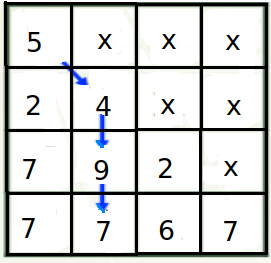
\includegraphics[width=100pt,height=100pt]{slike/dp-table-1.png}
		\caption{Primjer putanje pijuna. Ukupna vrijednost označene putanje iznosi 25.}
		\label{fig:pijun-putanja}
	\end{figure}
	
	Problem posjeduje optimalnu podstrukturu, jer optimalna putanja do polja $(i,j)$ mora sadržavati optimalnu putanju do jednog od polja iz kojih je moguće doći u $(i,j)$.
	
	Definišimo matricu $M$ tako da vrijednost $M(i,j)$ predstavlja maksimalnu sumu koja se može ostvariti na putanji od početnog polja $(0,0)$ do polja $(i,j)$.
	
	Da bismo izračunali vrijednost $M(i,j)$, posmatramo dva moguća prethodna polja:
	
	\begin{itemize}
		\item polje $(i-1,j)$;
		\item polje $(i-1,j-1)$.
	\end{itemize}
	
	Ako je pijun stigao iz jednog od tih polja, tada važi rekurzivna relacija:
	
	\begin{equation}
		M(i,j)=a_{ij}+\max\{M(i-1,j),\,M(i-1,j-1)\}.
	\end{equation}
	
	Bazni slučaj definisan je sa:
	
	\begin{equation}
		M(0,0)=a_{00}.
	\end{equation}
	
	Za pozicije koje nisu dostupne pijunu (npr. izvan granica matrice) možemo postaviti vrijednost $-\infty$, kako nikada ne bi bile odabrane kao dio optimalne putanje. 	Nakon popunjavanja matrice $M$, optimalna vrijednost rješenja dobija se kao:
	
	\begin{equation}
		\max_{0 \leq j < n} M(n-1,j),
	\end{equation}
	
	odnosno kao najveća vrijednost u posljednjem redu matrice $M$.  Na ovaj način svaki podproblem rješava se tačno jednom, pa je vremenska složenost algoritma jednaka $O(n^2)$, dok je potrebni memorijski prostor takođe $O(n^2)$.
	
\end{solution}


Implementacija ovog rješenje je data sljedećim k\^odom (pristup odozgo prema dolje).

\begin{minted}[fontsize=\footnotesize,scale=0.8]{python}
	A = None #matrica sa svim -1
	def init(n):
        
            A = [ [-1] * n for _ in range(n)  ]
            A[0][0] = M[0][0] #bazni slučaj
	
	def solve(k, l):# najbolji put od (0.0) do (k, l)
	    
	    for i in range(1, k):
	        for j in range(0, l):
	            best = A[i-1][j]  
	            if j>0:
	                best = max(best,  A[i-1][j-1])
	        A[i][j] = best + A[i][j]
	   
	    return A[k][l]

	#instanca
	M=[[4, 5, 7, 0],
    	[2, 3, 1, 3],
    	[1, 1, 3, 1],
    	[2, 3, 3, 3]
        ]	

	max_sum_path = 0
	for j in range(len(M)):
		init(len(A))
	        A = solve(len(A)-1, j)
		max_sum_path = max(max_sum_path, A[len(A)-1, j])
	
	#ispis rezultata	
	print(max_sum_path)
\end{minted}

\textit{Kompleksnost algoritma}. Funkcija \texttt{solve}() se izvršava u vremenu od $O(n^2)$   kao najzahtjevniji dio implementacije. Spoljašnja petlja se izvršava $n$ puta.  Prema tome, ukupna kompleksnost algoritma je $O(n^2 \cdot n)=O(n^3)$.

\end{solution}



\begin{example}
	Riješiti problem ruksaka primjenom dinamičkog programiranja.
\end{example}

\begin{solution}
	
	Posmatrajmo klasični problem ruksaka ($0$--$1$ ruksak). Ponovimo, neka je dato $n$ proizvoda, pri čemu proizvod $i$ ima težinu $w_i$ sa vrijednosti $p_i$,  $i=1,\ldots,n$. Kapacitet ruksaka iznosi $C$.
	
	\medskip
	
	\textit{Definisanje podproblema.} Neka $\textrm{DP}[i][j]$ čuva optimalnu vrijednost koju je moguće ostvariti korištenjem prvih $i$ proizvoda, za raspoloživi kapacitet ruksaka jednak $j$.  Dakle, podproblem je određen parom indeksa $
	(i,j), 
	i \in \{0,1,\ldots,n\}, 
	j \in \{0,1,\ldots,C\}.$
	
	\medskip
	
	\textit{Rekurzivna relacija.} Posmatrajmo podproblem $(i,j)$.	Postoje dva moguća slučaja:
	
	\begin{enumerate}
		\item Proizvod $i$ ne ulazi u optimalno rješenje. Tada je
	    $  \textrm{DP}[i][j] = \textrm{DP}[i-1][j].$
		\item Proizvod $i$ ulazi u optimalno rješenje. To je moguće samo ako je njegova težina manja ili jednaka raspoloživom kapacitetu, odnosno ako važi $w_i \leq j$. U tom slučaju ostvarujemo vrijednost $p_i$, a preostali kapacitet postaje $j-w_i$. Tada je
		$$
		\textrm{DP}[i][j] =\max\{ \textrm{DP}[i-1][j-w_i] + p_i, \textrm{DP}[i-1][j] \}.
		$$
		
	\end{enumerate}
	
	Birajući bolje od ova dva rješenja, dobijamo rekurzivnu relaciju:
	
	$$
	\textrm{DP}[i][j] =
	\begin{cases}
		\max\bigl(\textrm{DP}[i-1][j],\textrm{DP}[i-1][j-w_i] + p_i\bigr),
		& \text{ako } w_i \leq j, \\
		\textrm{DP}[i-1][j],
		& \text{ako } w_i > j.
	\end{cases}
	$$
	\medskip
	
	\textit{Bazni slučajevi.} Ako je kapacitet ruksaka jednak nuli, nijedan proizvod ne može biti odabran, pa vrijedi $
	\textrm{DP}[i][0]=0, i=0,\ldots,n.$  Takođe, ako ne razmatramo nijedan proizvod, maksimalna ostvariva vrijednost jednaka je nuli bez obzira na kapacitet: $\textrm{DP}[0][j]=0, j=0,\ldots,C.$
	
	\medskip
	
	\textit{Konačno rješenje.}	Nakon popunjavanja matrice $\textrm{DP}$, optimalna vrijednost problema nalazi se u ćeliji $
	\textrm{DP}[n][C].$	Drugim riječima, ona predstavlja najveću moguću vrijednost koju možemo smjestiti u ruksak kapaciteta $C$ razmatrajući svih $n$ proizvoda.
	
	\medskip
	
	\textit{Složenost algoritma.}  Matrica $\textrm{DP}$ sadrži $(n+1)(C+1)$ elemenata, a svaka ćelija se računa u konstantnom vremenu. Zbog toga je vremenska složenost algoritma $ O(n \cdot C),$ dok je prostorna složenost takođe $O(n \cdot C).$
	
\end{solution}
  \\
	 
	 Implementacija paradigme dinamičkog programiranja za rješavanje pro\-blema ruksaka je data narednim k\^odom.
	 
	 \begin{minted}[fontsize=\footnotesize,scale=0.8]{python}
	 def knapsack(n, C, W, p):
	 	DP = [[0 for x in range(C + 1)] for x in range(n + 1)]
	 
	 	# tabuliranje
	 	for i in range(n + 1):
	 		for j in range(C + 1):
	 			if i == 0 or j == 0:
	 				DP[i][j] = 0
	 			elif W[i-1] <= j:
	 				DP[i][j] = max(p[i-1]
	 				       +DP[i-1][j-W[i-1]],
	 				        DP[i-1][j])
	 			else:
	 				DP[i][j] = {DP}[i-1][j]
	 
	 	return DP[n][C]
	 
	 #instanca:
	 p = [60, 100, 120]
	 W = [10, 20, 30]
	 C = 50
	 n = len(p)
	 #poziv funkcije
	 print knapsack(n, C, W, p, n)
	 \end{minted}
	 
 \textit{Kompleksnost algoritma}. Najskuplji dio algoritma su dvije ugnježdene \texttt{for} petlje, koje izvršavaju $O(n \cdot C)$ iteracija. Svaka od iteracija se izvršava u konstantnom vremenu, pa je i ukupna kompleksnost algoritma jednaka $O(n \cdot C)$.
\end{solution}

Navedimo sada primjer konkretne instance problema i način popunjavanja DP tabele.

Neka je broj proizvoda $n=4$, kapacitet ruksaka $C=5$, a težine i vrijednosti proizvoda date nizovima $W=(2,3,4,5), P=(3,4,5,6).$

Formiramo matricu $\textrm{DP}$ dimenzija $(n+1)\times(C+1)$, pri čemu vrijednost $\textrm{DP}[i][j]$ predstavlja maksimalnu vrijednost koju je moguće ostvariti korištenjem prvih $i$ proizvoda i ruksaka kapaciteta $j$.

\medskip

Prvi korak sastoji se od inicijalizacije baznih slučajeva. Kako ruksak kapaciteta $0$ ne može sadržavati nijedan proizvod, vrijedi $\textrm{DP}[i][0]=0$ za sve $i$. Takođe, ako ne razmatramo nijedan proizvod, ostvarena vrijednost je jednaka nuli, pa vrijedi $\textrm{DP}[0][j]=0$ za sve $j$. Dobijamo početnu tabelu:

\begin{table}[H]
	\centering
	\begin{tabular}{|c|cc|cccccc|}\hline
		$j\rightarrow$ & Proizvod & & 0 & 1 & 2 & 3 & 4 & 5 \\ \hline
		$i=0$ & & & 0 & 0 & 0 & 0 & 0 & 0 \\
		$i=1$ & $w_1=2$ & $p_1=3$ & 0 & & & & & \\
		$i=2$ & $w_2=3$ & $p_2=4$ & 0 & & & & & \\
		$i=3$ & $w_3=4$ & $p_3=5$ & 0 & & & & & \\
		$i=4$ & $w_4=5$ & $p_4=6$ & 0 & & & & & \\ \hline
	\end{tabular}
\end{table}

\medskip

Za $i=1$ razmatramo samo prvi proizvod. Kako njegova težina iznosi $2$, nije ga moguće smjestiti u ruksak kapaciteta $0$ ili $1$. Za sve kapacitete $j\geq 2$ optimalno je uzeti taj proizvod, pa druga vrsta tabele postaje:

\begin{table}[H]
	\centering
	\begin{tabular}{|c|cc|cccccc|}\hline
		$j\rightarrow$ & Proizvod & & 0 & 1 & 2 & 3 & 4 & 5 \\ \hline
		$i=0$ & & & 0 & 0 & 0 & 0 & 0 & 0 \\
		$i=1$ & $w_1=2$ & $p_1=3$ & 0 & 0 & 3 & 3 & 3 & 3 \\
		$i=2$ & $w_2=3$ & $p_2=4$ & 0 & & & & & \\
		$i=3$ & $w_3=4$ & $p_3=5$ & 0 & & & & & \\
		$i=4$ & $w_4=5$ & $p_4=6$ & 0 & & & & & \\ \hline
	\end{tabular}
\end{table}

\medskip

Dalje popunjavamo treću vrstu ($i=2$), pri čemu su na raspolaganju prva dva proizvoda.

\begin{table}[H]
	\centering
	\begin{tabular}{|c|cc|cccccc|}\hline
		$j\rightarrow$ & Proizvod & & 0 & 1 & 2 & 3 & 4 & 5 \\ \hline
		$i=0$ & & & 0 & 0 & 0 & 0 & 0 & 0 \\
		$i=1$ & $w_1=2$ & $p_1=3$ & 0 & 0 & 3 & 3 & 3 & 3 \\
		$i=2$ & $w_2=3$ & $p_2=4$ & 0 & 0 & 3 & 4 & 4 & 7 \\
		$i=3$ & $w_3=4$ & $p_3=5$ & 0 & & & & & \\
		$i=4$ & $w_4=5$ & $p_4=6$ & 0 & & & & & \\ \hline
	\end{tabular}
\end{table}

Razmotrimo ćeliju $\textrm{DP}[2][4]$. Postoje dvije mogućnosti:

\begin{itemize}
	\item ne uzimamo drugi proizvod, pa je vrijednost jednaka $\textrm{DP}[1][4]=3$;
	\item uzimamo drugi proizvod, pa preostaje kapacitet $4-3=1$, odnosno dobijamo vrijednost $\textrm{DP}[1][1]+4=0+4=4.$
\end{itemize}

Prema tome, $\textrm{DP}[2][4]=\max\{3,4\}=4.$ Vrijednost $\textrm{DP}[2][5]=7$ dobija se uzimanjem oba proizvoda, jer vrijedi $\textrm{DP}[1][2]+4 = 3+4 = 7.$

\medskip

Popunjavanjem četvrte vrste ($i=3$) dobijamo:

\begin{table}[H]
	\centering
	\begin{tabular}{|c|cc|cccccc|}\hline
		$j\rightarrow$ & Proizvod & & 0 & 1 & 2 & 3 & 4 & 5 \\ \hline
		$i=0$ & & & 0 & 0 & 0 & 0 & 0 & 0 \\
		$i=1$ & $w_1=2$ & $p_1=3$ & 0 & 0 & 3 & 3 & 3 & 3 \\
		$i=2$ & $w_2=3$ & $p_2=4$ & 0 & 0 & 3 & 4 & 4 & 7 \\
		$i=3$ & $w_3=4$ & $p_3=5$ & 0 & 0 & 3 & 4 & 5 & 7 \\
		$i=4$ & $w_4=5$ & $p_4=6$ & 0 & & & & & \\ \hline
	\end{tabular}
\end{table}

Na primjer, za ćeliju $\textrm{DP}[3][4]$ imamo $\textrm{DP}[2][4]=4$ ako ne uzmemo treći proizvod, odnosno $\textrm{DP}[2][0]+5=5$ ako ga uzmemo. Zato je $\textrm{DP}[3][4]=\max{4,5}=5.$

\medskip

Konačno, nakon obrade četvrtog proizvoda dobijamo završnu tabelu:

\begin{table}[H]
	\centering
	\begin{tabular}{|c|cc|cccccc|}\hline
		$j\rightarrow$ & Proizvod & & 0 & 1 & 2 & 3 & 4 & 5 \\ \hline
		$i=0$ & & & 0 & 0 & 0 & 0 & 0 & 0 \\
		$i=1$ & $w_1=2$ & $p_1=3$ & 0 & 0 & 3 & 3 & 3 & 3 \\
		$i=2$ & $w_2=3$ & $p_2=4$ & 0 & 0 & 3 & 4 & 4 & 7 \\
		$i=3$ & $w_3=4$ & $p_3=5$ & 0 & 0 & 3 & 4 & 5 & 7 \\
		$i=4$ & $w_4=5$ & $p_4=6$ & 0 & 0 & 3 & 4 & 5 & 7 \\ \hline
	\end{tabular}
\end{table}

Posmatrajmo ćeliju $\textrm{DP}[4][5]$. Ako ne uzmemo četvrti proizvod, vrijednost je $ \textrm{DP}[3][5]=7.$ Ako ga uzmemo, dobijamo $\textrm{DP}[3][0]+6=6.$ Stoga je $ \textrm{DP}[4][5]=\max\{7,6\}=7.$

Kako se optimalna vrijednost problema nalazi u ćeliji $\textrm{DP}[n][C]$, zaključujemo da je optimalna vrijednost za posmatranu instancu jednaka $\textrm{DP}[4][5]=7.$  Ona se ostvaruje odabirom prvog i drugog proizvoda, čija je ukupna težina $2+3=5$, a ukupna vrijednost $3+4=7$.

 \begin{definition}
 	String $s$ je podniz stringa $s_1$ akko se $s$ može dobiti brisanjem (nula ili više)
 	karaktera iz stringa $s_1$ a čuvajući poredak ostalih karaktera. \\
 	Npr.  \texttt{acd} je podniz stringa \texttt{abbbcdef}.   Prefiks stringa $s$ dužine $k$ je podstring stringa $s$ koji se sastoji od prvih $k$ karaktera. Npr. prefiks dužine tri stringa \texttt{abbbcdef} je string \texttt{abb}. 
 	
 \end{definition}
 
\begin{example}
	(\textit{Problem najdužeg zajedničkog podniza} (eng. \emph{Longest Common Subsequence Problem} -- LCS)). Neka su data dva stringa $s_1$ i $s_2$. Potrebno je odrediti najduži string $s$ koji je podniz oba ulazna stringa.
	
	Na primjer, za stringove $s_1=\texttt{aatdccddc}$ i 
	$s_2=\texttt{agccddta} $
	jedno optimalno rješenje je $s=\texttt{accdd},$
	čija je dužina jednaka $5$.
\end{example}

\begin{solution}
	
	Definišimo podproblem parom indeksa $(i,j)$, gdje je
	$0 \leq i \leq |s_1|, 0 \leq j \leq |s_2|.
	$ 
	Podproblem označen parom $(i,j)$ odgovara određivanju dužine najdužeg zajedničkog podniza između prefiksa od $s_1$ dužine $i$ i prefiksa od $s_2$ dužine $j$.  Rješenja podproblema memorišemo u matrici $\textrm{DP}$, pri čemu vrijednost $\textrm{DP}[i][j]$ predstavlja dužinu najdužeg zajedničkog podniza pomenutih prefiksa.
	
	\medskip
	
	\textit{Rekurzivna relacija.} Posmatrajmo posljednje karaktere razmatranih prefiksa, odnosno karaktere $s_1[i-1]$ i $s_2[j-1]$. Moguća su dva slučaja.
	
	\begin{itemize}
		\item Ako je
		$s_1[i-1]=s_2[j-1],$
		tada taj karakter može biti dio optimalnog rješenja. Optimalni podniz podproblema $(i,j)$ dobija se proširivanjem optimalnog rješenja podproblema $(i-1,j-1)$ za jedan karakter. Stoga vrijedi $\textrm{DP}[i][j]=\textrm{DP}[i-1][j-1]+1.$
		
		\item Ako je $ s_1[i-1]\neq s_2[j-1],$
		tada barem jedan od ta dva karaktera neće generisati optimalno rješenje. Zbog toga razmatramo dva podproblema 
		$ (i-1,j)$ i
		$(i,j-1)$,
		odnosno izostavljamo posljednji karakter prvog ili drugog prefiksa. Optimalna vrijednost dobija se izborom boljeg od ta dva podproblema:
		$$ \textrm{DP}[i][j]
		=
		\max\{\textrm{DP}[i-1][j],\,\textrm{DP}[i][j-1]\}.
		$$
	\end{itemize}
	
	Prema tome, rekurzija ima oblik
	
	$
	\textrm{DP}[i][j]=
	\begin{cases}
		\textrm{DP}[i-1][j-1]+1, & \text{ako je } s_1[i-1]=s_2[j-1], \\
		\max\{\textrm{DP}[i-1][j],\textrm{DP}[i][j-1]\}, & \text{inače}.
	\end{cases}
	$
	
	\medskip
	
	\textit{Bazni slučajevi.} Ako je jedan od prefiksa prazan, tada zajednički podniz ne postoji, pa je njegova dužina jednaka nuli. Zbog toga vrijedi  $\textrm{DP}[i][0]=0,
	  0\leq i\leq |s_1|,$ i $
	\textrm{DP}[0][j]=0,
	0\leq j\leq |s_2|.$
	
	\medskip
	
	Nakon popunjavanja matrice $\textrm{DP}$, dužina najdužeg zajedničkog podniza nalazi se u ćeliji $\textrm{DP}[|s_1|][|s_2|].$ Sam podniz može se rekonstruisati prolaskom unazad kroz matricu, počevši od pozicije $(|s_1|,|s_2|)$ i prateći odluke koje su dovele do optimalne vrijednosti.
	
\end{solution}

	    
	 Implementacija paradigme dinamičkog programiranja za rješavanje LCSP je data narednim k\^odom. 
 \begin{minted}[fontsize=\footnotesize,scale=0.8]{python}
	    	
	     def LCS(s1, s2): #tabuliranje
	    	      
	    	  if len(s1)==0 or len(s2)==0:
	    	     return 0
	    	     
	    	  DP = [ [0]*(len(s2)+1) for _ in range(len(s1)+1)]
	              for i in range(1, len(s1)+1):
	    	      for j in range(1, len(s2)+1):
	    		     if s1[i-1] == s2[j-1]: 
	    		         DP[i][j] = DP[i-1][j-1] + 1
	    		     else:
	    		         DP[i][j] = max(DP[i-1][j], DP[i][j-1])
	    	  return DP[len(s1)][len(s2)]        
	    		           
	    	      
	     #instanca:
	     s1 = "abcdcdcdaa"
	     s2 = "abbaabcccddd"
	     #poziv DP metoda
	     lcs = LCS(s1, s2)
	     print("Duzina LCS-a je: ", lcs)     
 \end{minted}
	     Primijetimo da implementacija koristi princip odozdo-nagore.
	     
	     \textit{Kompleksnost algoritma}. Dvije \texttt{for}-petlje  izvršavaju ukupno $O(|s_1|\cdot |s_2|)$ iteracija. Svaka od iteracija se izvršava u konstantnom vremenu, pa je shodno tome ukupno vrijeme izvršavanja algoritma jednako $O(|s_1| \cdot |s_2|)$. Ako je $n = \max\{|s_1|, |s_2|\}$, dobija se kvadratna $O(n^2)$ kompleksnost. 
	     
	     %\begin{figure}[H]
	     %	\centering
	     %	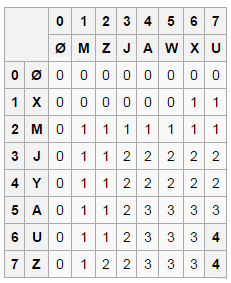
\includegraphics[width=150pt,height=150pt]{slike/dp-lcs-table.png}
	     %	\caption{DP matrica za dva stringa $s_1=$\texttt{MZJAWXU} i $s_2=$\texttt{XMJYAUZ}. Rješenje je dužine 4 (pogledati donji desni ugao matrice). }
	     %\end{figure}
     
     \begin{table}
     	  \centering
     	  \begin{tabular}{cc|cccccccc}
     	  	& & 0&1 &2 &3 &4 &5 &6 &7   \\
     	  
     	  	& & $\emptyset$&\texttt{M} &\texttt{Z} &\texttt{J} &\texttt{A} &\texttt{W} &\texttt{X} &\texttt{U}  \\ \hline \hline
     	  	
     	  	0&$\emptyset$ &0& 0& 0&  0&0 &0 & 0   & 0 	   \\
     	  	1& \texttt{X}& 0& 0& 0& 0& 0& 0&  1  & 1                \\	
     	  	2& \texttt{M}& 0& 1& 1& 1& 1& 1&  1  & 1                \\	
     	  	3& \texttt{J}& 0& 1& 1& 2& 2& 2&  2  & 2                \\	
     	  	4& \texttt{Y}&0 & 1& 1& 2& 2& 2&  2  & 2                 \\	
      	  	5& \texttt{A}& 0& 1& 1& 2& 3& 3&  3  & 3                \\	
      	  	6& \texttt{U}& 0& 1& 1& 2& 3& 3&  3  & 4                \\	
      	  	7& \texttt{Z}& 0& 1& 2& 2& 3& 3&  3  & 4                \\	 \hline \hline
     	  \end{tabular}
 	 \caption{DP matrica za LCSP dva stringa $s_1=$\texttt{MZJAWXU} i $s_2=$\texttt{XMJYAUZ}. Rješenje je dužine 4 (pogledati donji desni ugao matrice). }  \label{tab:dp-lcs-example} 
 	\end{table}
\end{solution}

%https://www.programiz.com/dsa/longest-common-subsequence ==> primjer tabele sa rješenjem...

\begin{example} \textbf{Problem sume podskupa} (eng. \emph{Subset Sum Problem}). Neka je dat niz od $n$ nenegativnih cijelih brojeva i ciljna vrijednost \textit{sum}. Potrebno je odrediti da li postoji podskup elemenata datog niza čiji je zbir jednak vrijednosti \textit{sum}.
\end{example}

\begin{solution}
	
	Posmatrajmo primjer u kojem je $
	niz=[1,7,8,2,6]
	$ i  $sum=9.$
	
		Odgovor je pozitivan, jer podskup ${1,2,6}$ ima zbir jednak $9$.
	
	\medskip
	
	Da bismo riješili problem dinamičkim programiranjem, definišimo podproblem određen parom indeksa
	
	$$
	(i,j),
	0 \leq i \leq n,
	0 \leq j \leq sum.
	$$
	
	Podproblem $(i,j)$ odgovara pitanju:
	
	\begin{quote}
		Da li među prvih $i$ elemenata niza postoji podskup čiji je zbir jednak $j$?
	\end{quote}
	
	Rješenja podproblema memorišemo u matrici $\textrm{DP}$, gdje je
	
	$$
	\textrm{DP}[i][j]=
	\begin{cases}
		True, & \text{ako takav podskup postoji},\\
		False, & \text{inače}.
	\end{cases}
	$$
	
	\medskip
	
	\textit{Rekurzivna relacija.} 	Posmatrajmo podproblem označen parom $(i,j)$ i element $niz[i-1]$. Postoje dva moguća slučaja.
	
	\begin{itemize}
		\item {Element $niz[i-1]$ pripada rješenju.}
		
		U tom slučaju preostali elementi moraju formirati zbir $j-niz[i-1].$	Stoga vrijedi $\textrm{DP}[i][j] = \textrm{DP}[i-1][j-niz[i-1]],$
		pod uslovom da je $
		j \geq niz[i-1].$
		
		\item {Element $niz[i-1]$ ne uzimamo u rješenje.} Tada se problem svodi na prvih $i-1$ elemenata:
		$ \textrm{DP}[i][j] = \textrm{DP}[i-1][j].$
		
	\end{itemize}
	
	Pošto je dovoljno da bude zadovoljen bilo koji od ova dva slučaja, dobijamo rekurziju
	
	$$
	\textrm{DP}[i][j]=
	\textrm{DP}[i-1][j] \vee \textrm{DP}[i-1][j-niz[i-1]],$$
	ako je $j \geq niz[i-1].$	U suprotnom, element ne može biti dio rješenja, pa vrijedi $\textrm{DP}[i][j] =	\textrm{DP}[i-1][j].$
	
	\medskip
	
	\textit{Bazni slučajevi.}  	Zbir $0$ uvijek možemo ostvariti izborom praznog podskupa, pa vrijedi $
	\textrm{DP}[i][0]=True, 
	0\leq i\leq n.$ 	S druge strane, ako ne raspolažemo niti jednim elementom, nijedan pozitivan zbir ne može biti formiran $ \textrm{DP}[0][j]=False, 1\leq j\leq sum.
	$
	
	\medskip
	
	Nakon popunjavanja matrice $\textrm{DP}$, odgovor na početni problem nalazi se u ćeliji $\textrm{DP}[n][sum].$
	
	Ako je vrijednost ove ćelije \textit{True}, postoji podskup čiji je zbir jednak zadanoj vrijednosti \textit{sum}; u suprotnom takav podskup ne postoji.
	
\end{solution}

   
    Implementacija paradigme dinamičkog programiranja za rješavanje Pro\-blema \emph{sume podskupa} je data narednim k\^odom. 
   
   \begin{minted}[fontsize=\footnotesize,scale=0.8]{python}
   	  def sum_array(niz, suma):
   	      #tabulation:
   	      DP = [[False] * (suma +1) for _ in range(len(niz) + 1) ]
   	      for i in range(len(niz)+1):
   	          DP[i][0] = True
   	      
   	      for i in range(1, len(niz)+1):   
   	          for j in range(1, suma+1):
   	              if j >= niz[i-1]:
   	                 DP[i][j] = DP[i-1][j-niz[i-1]] or DP[i-1][j]
   	              else:
   	                 DP[i][j] = DP[i-1][j]
   	                 
   	      return DP[len(niz)][suma]
   	  
   	  #instanca:
   	  niz = [3, 34, 4, 12, 5, 2]
   	  suma = 9
   	  postoji = sum_array(niz, suma)
   	  print("Postoji podskup sa sumom" if postoji else  
   	        "Ne postoji podskup sa sumom")
   \end{minted}
\end{solution}
Primijetimo da smo dinamičko programiranje implementirali pomoću pristupa \textit{odozdo prema gore} (tabuliranje). 

Implementirajmo sada dinamičko programiranje za ovaj problem pristupom \textit{odozgo prema dolje}.

   \begin{minted}[fontsize=\footnotesize,scale=0.8]{python}
	def init(niz, suma):
		global DP
		DP = [[-1] * (suma + 1) for _ in range(len(niz) + 1) ]
	
	
	def sum_array_top_down(niz, suma, i, j, DP = [ ]):
	
		if DP[i][j] != -1:
			return DP[i][j]
	
		if j == 0:
			DP[i][0] = True
			return True 
		if i == 0: 
			DP[0][j] = False
			return False
		#recursion: 
		if j >= niz[i-1]:  
			DP[i][j] = sum_array_top_down(niz, suma, i-1, j, DP) or
			sum_array_top_down(niz, suma, i-1, j-niz[i-1], DP)
			return DP[i][j]
		else:
			DP[i][j] = sum_array_top_down(niz, suma, i-1, j, DP)
			return DP[i][j]
\end{minted}  

\textit{Kompleksnost algoritma}. Broj iteracija koje se izvršavaju je jednak $O(n \cdot sum)$. Svaka iteracija se izvršava u konstantnom vremenu, pa je i ukupna kompleksnost algoritma jednaka  $O(n \cdot sum)$. Dakle, ako je vrijednost \emph{sum} ogromna, ekponencijalno velika u odnosu na veličinu niza, ovakav algoritam će biti neefikasan. 

\begin{example}
	(\textit{Problem rezanja štapa}). Dat je štap dužine $n$ i niz cijena \textit{price}, pri čemu \textit{price}$[i-1]$ predstavlja cijenu štapa dužine $i$, za svako $1 \leq i \leq n$.\\ 
	
	Potrebno je odrediti način rezanja štapa na manje dijelove tako da ukupan ostvareni profit bude maksimalan.
	
\end{example}

\begin{solution}
	
	Posmatrajmo primjer instance problema date sa 
	$$price = [1,5,8,9,10,17,17,20].$$ 
	Pretpostavimo da je dužina štapa $n=4.$	Ako se štap ne reže, ostvaruje se profit jednak $9$. Međutim, ako ga podijelimo na dva dijela dužine $2$, dobijamo profit $
	5+5=10,
	$ što predstavlja bolje (u ovom slučaju optimalno) rješenje za tu instancu.
	
	\medskip
	
	Da bismo problem riješili dinamičkim programiranjem, definišimo podproblem dužinom štapa $i$, gdje je $
	0 \leq i \leq n.
	$
	
	Neka $\textrm{DP}[i]$ označava maksimalni profit koji se može ostvariti rezanjem štapa dužine $i$. Vrijednost $\textrm{DP}[i]$ memorišemo u nizu $\textrm{DP}$ na poziciji $i$.
	
	\medskip
	
	\textit{Rekurzivna relacija.} Posmatrajmo štap dužine $i$. Podijelimo ovaj štap na dio dužine $k$, gdje je $ 1 \leq k \leq i.$ Na taj način štap dijelimo na:
	
	\begin{itemize}
		\item dio dužine $k$, čija je vrijednost $price[k-1]$;
		\item preostali dio dužine $i-k$, čiji je optimalni profit jednak $\textrm{DP}[i-k]$.
	\end{itemize}
	
	Za svaku moguću vrijednost $k$ dobijamo kandidatsko rješenje $price[k-1] + \textrm{DP}[i-k].$  Optimalna vrijednost za štap dužine $i$ dobija se izborom najboljeg među svim mogućim prvim rezovima:
	
	$$
	  \textrm{DP}[i] =
	  \max_{1 \leq k \leq i}
	  \left\{
		price[k-1] + \textrm{DP}[i-k]
		\right\}.
	$$
	
	\medskip
	
	\textit{Bazni slučaj.} Štap dužine $0$ nema vrijednost, pa vrijedi $\textrm{DP}[0]=0.$
	
	\medskip
	
	Nakon popunjavanja niza $\textrm{DP}$, optimalna vrijednost početnog problema nalazi se u ćeliji $
	\textrm{DP}[n].$ 	Vrijednost $\textrm{DP}[n]$ predstavlja maksimalan profit koji se može ostvariti rezanjem štapa dužine $n$.
	
	\medskip
	
	\textit{Vremenska složenost.}	Za svaku dužinu $i$ razmatra se najviše $i$ mogućih pozicija prvog reza. Ukupan broj operacija jednak je $	\sum_{i=1}^{n} i =
	\frac{n(n+1)}{2},
	$  pa je vremenska složenost algoritma $O(n^2).$  Prostorna složenost iznosi $O(n),$ jer se koristi jednodimenzionalni niz $\textrm{DP}$ veličine $n+1$.
	
\end{solution}


 Implementacija paradigme dinamičkog programiranja za rješavanje problema  rezanja štapa je data narednim k\^odom. 
 
 \begin{minted}[fontsize=\footnotesize,scale=0.8]{python}
	def stick_cut(d, price):

		DP = [-1] * (d+1)  #init
		DP[0], DP[1] = 0, price[0]

		for i in range(2, d+1):
			for k in range(1, i+1):
				if DP[i] < DP[i-k] + price[k-1]: 
					DP[i] =  DP[i-k] + price[k-1]
		return DP[d]       
     
     #instanca
     d = 4
     price = [1, 5, 8, 9, 10, 17, 17, 20] 
     max_profit = stick_cut(d, price)     
     #poziv
     print(max_profit)
 \end{minted} 
\textit{Napomena}. Pogledajmo drvo rekurzije koje se kreira algoritmom grube sile na Slici~\ref{fig:brute-force-stick-cut}  pri rješavanju problema rezanja štapa za $d=4$. Ovaj pristup enumeriše sva moguća rješenja za rezanje štapa dužine $d=4$. Prvo uzima cio štap u razmatranje (i njegovu cijenu), zatim otkida dio štapa dužine 1, dok se ostatak štapa (dužine 3) rješava (dijeli) rekurzivno itd. Kompletno rješenje dobijamo u listovima stabla (označeni sa 0). 
\begin{center}
	\begin{figure}[H]
		\centering
		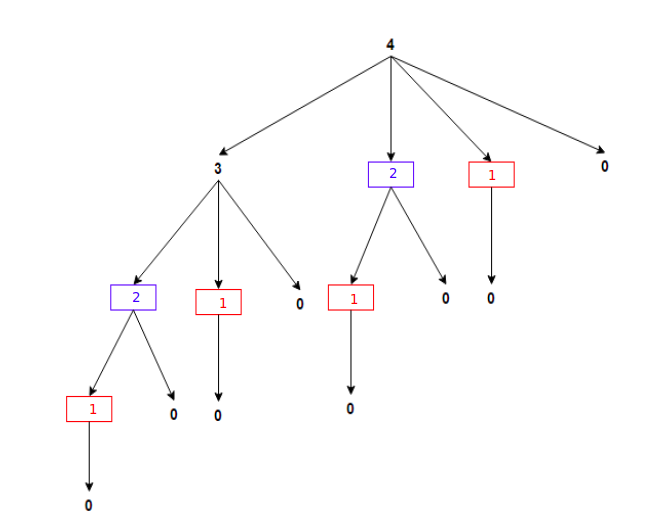
\includegraphics[width=300pt,height=230pt]{slike/brute-force-cutting-stick.png}
		
		\caption{Drvo grananja paradigme grube sile za rješavanje problema rezanja štapa.}\label{fig:brute-force-stick-cut}
	\end{figure}
\end{center}



  Npr. put koji posjećuje čvorove sa oznakama 4 $\rightarrow$ 3 $\rightarrow$ 2 $\rightarrow$ 1 $\rightarrow$ 0, odgovara rješenju u kojem se štap siječe na 4 manja štapa dužine 1 (cijene $4 \times price[0]$). Slično, za put koji posjećuje čvorove sa oznakama 4 $\rightarrow$ 3 $\rightarrow$ 1 $\rightarrow$ 0, odgovara rješenju u kojem se štap sječe na dva manja štapa dužine 1, te jedan dužine 2 (cijene $2 \times price[0] + price[1]$).   
  
   Jasno se vidi da se podproblemi isprepliću, tj. da se, npr. rješavanje problema štapa dužine dva računa više (dva) puta. U slučaju dinamičkog programiranja implementiran  pristupom odozgo prema dolje, stablo će biti značajno redukovano, jer neće postojati rekalkulacije istih podproblema (dakle, nema identičnih kopija podstabala u DP stablu). 
 

\section*{Zadaci}

\begin{enumerate}
	\item Riješiti problem trgovačkog putnika pomoću algoritamske paradigme grube sile.
	\item Riješiti problem ruksaka pomoću algoritamske paradigme grube sile.
	\item Dati  su brojevi  $0 \leq  M  <  N  \leq  1,000,000$. Odrediti  najmanji  broj  sastavljen  samo  od 
	neparnih cifara, koji pri dijeljenju sa $N$ daje ostatak $M$. Ukoliko traženi broj ne postoji, vratiti $−1$. 
	
	 \item Neka su dati prirodni brojevi $n$, koji označava broj promjenljivih, i $s$, koji označava sumu promjenljivih. Uz
pomoć rekurzivnih algoritama napisati program koji pronalazi sva moguća rješenja
za promjenljive  kojih ima $n$ i  čija   suma treba biti jednaka $ s$. 

\textit{Instanca}: $n = 5, s = 4$;
\textit{Rješenje}: 70. \\
\textit{Napomena}.
Instanca predstavlja jednačinu $x_1 + x_2 + x_3 + x_4 + x_5 = 4, x_i \in \mathbb{N}$. 
Sva moguća rješenja su:
$(1\ 1\ 1\ 1\ 0), (1\ 0\ 1\ 1\ 1), (0\ 1\ 1\ 1\ 1), \ldots ,$ $(2\ 1\ 0\ 0\ 1), \ldots , (2\ 2\ 0\ 0\ 0)$ itd.
	%pohlepni algoritmi (dva zadatka) 
	%https://www.geeksforgeeks.org/minimum-product-subset-array/
	\item Pronaći podskup elemenata niza tako da  proizvod elemenata u podskupu bude minimalan. Koristiti paradigmu pohlepnih algoritama.\\
	 \textit{Instanca}: $niz = [ -1, -1, -2, 4, 3]$; \textit{Rješenje}:  -24 ($=(-2 )\cdot (-1) \cdot (-1) \cdot 4 \cdot 3$). 
	
	%https://www.geeksforgeeks.org/greedy-algorithm-egyptian-fraction/
	\item Svaki pozitivan razlomak možemo predstaviti kao zbir jedi\-nstvenih jediničnih razlomaka. Razlomak je jedinični ako je brojnik 1, a nazivnik pozitivan cijeli broj; npr. $1/3$ je jedinični razlomak. Npr. $2/3= 1/2 + 1/6, 3/7=1/3 + 1/11 + 1/231.$   Uz pomoć paradigme pohlepnih algoritama, za proizvoljan razlomak, naći jedinične razlomke koje u zbiru daju taj razlomak.  
	
	
	\item Riješiti problem nalaska najdužeg zajedničkog podniza dva stringa pomoću dinamičkog programiranja pristupom odozgo prema dolje. 
	
	\item U ulazu je dat niz brojeva.  Konstruisati algoritam dinamičkog programi\-ranja koji daje odgovor na pitanje li postoji particionisanje niza na dva (disjunktna) skupa tako da je zbir elemenata u obje particije jednak.
	\item Implementirati metod dinamičkog programiranja  za problem rezanja štapa koristeći pristup odozgo prema dolje.
	
	\item Neka su u ulazu data dva stringa $s_1$ i $s_2$. Uz pomoć dinamičkog programi\-ranja, pronaći najkraći string $s$ tako da
	su stringovi $s_1$ i $s_2$ podnizovi stringa $s$.
	\item  Data  je riječ i riječnik (skup riječi). Ispitati da li se riječ može podijeliti na segmente (podstringove) tako da oni pripadaju riječniku. \\
	
	\textit{Instanca}: $$dict = \{\texttt{this}, \texttt{th}, \texttt{is}, \texttt{famous}, \texttt{Word}, \texttt{break}, \texttt{b}, \texttt{r}, \texttt{e}, \texttt{a}, \texttt{k},	\texttt{br}, \texttt{bre}, \texttt{brea}, \texttt{ak}, \texttt{problem} \} $$ te   $$word = \texttt{Wordbreakproblem}.$$  
	\textit{Rješenje}: \texttt{Word break problem},  kao jedno od rješenja.
	
	\item Neka je dat pravougaonik dimenzija $N\times M$. Pretpostavimo da je na raspolaganju beskonačan broj pločica
	formata $2^i \times 2^i$, $i = 0, 1, 2, 3, \ldots $. 
	
	Napisati program koji rekurzivno pronalazi minimalan broj pločica koji je potreban da bi se
	popločao pravougaonik datih dimenzija.
	
	\textit{Instanca}:  $N = 6, M=5$;	\textit{Rješenje}: 9 (pločica) -- vidjeti narednu sliku. %~\ref{fig:plocice}. 
	
	\begin{figure}[H]
	    \centering
		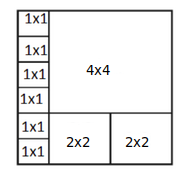
\includegraphics[width=120pt,height=100pt]{slike/plococe-dp-zadatak.png}
		\label{fig:plocice}
		\caption{Optimalno pokrivanje ploče 6 $\times$ 5}
	\end{figure}

\item Napisati program koji generiše sve mogućnosti da se stavi $+$ ili $-$ ili niti jedna od ove dvije opcije između brojeva $1,2,\ldots,9$ (ovim redom) tako da se kao rezultat izvršenja operacija dobije vrijednost 100. Npr. jedno takvo rješenje je $1 + 2 + 3 - 4 + 5 + 6 + 78 + 9 = 100$.
 
 \item Za dva stringa, napisati program koji ispisuje najkraći niz umetanja i brisanja karaktera u prvi string čijom se primjenom  dobija drugi string.
\end{enumerate}
\chapter[Primjena algoritamskih paradigmi na probleme iz aritmetike]{Primjena algoritamskih paradigmi na probleme iz aritmetike}

U ovoj glavi razmatramo primjenu algoritamskih paradigmi predstavljenih u prethodnom poglavlju na odabrane probleme iz aritmetike i teorije brojeva. Cilj je pokazati kako se različiti pristupi dizajnu algoritama, poput grube sile, podijeli-pa-zavladaj, dinamičkog programiranja i drugih paradigmi, mogu koristiti za efikasno rješavanje matematičkih problema.\\

%ISHODI UCENJA:

Nakon uspješnog savladavanja sadržaja ove glave student će biti u stanju da:

\begin{itemize}
	\item primijeni prethodno obrađene algoritamske paradigme na rješavanje
	problema iz elementarne aritmetike i teorije brojeva;
	
	\item objasni i implementira Eratostenovo sito za efikasno određivanje
	prostih brojeva u zadanom intervalu;
	
	\item implementira postupke faktorizacije cijelih brojeva i analizira
	njihovu vremensku složenost;
	
	\item izračunava binomne koeficijente primjenom rekurzivnog pristupa
	i dinamičkog programiranja te uporedi njihove performanse;
	
	\item objasni i implementira Hornerov metod za efikasno izračunavanje
	vrijednosti polinoma;
	
	\item analizira vremensku i prostornu složenost algoritama za razmatrane
	aritmetičke probleme i uporedi različite pristupe njihovom rješavanju.
\end{itemize}

\section{Eratostenovo sito}

\begin{definition}
	Broj $n \in \mathbb{N}$ naziva se \textit{prostim brojem} ako je djeljiv isključivo sa $1$ i samim sobom.
\end{definition}

Na primjer, prvih pet prostih brojeva su: $2, 3, 5, 7, 11.$ Broj $6$ nije prost jer je, pored brojeva $1$ i $6$, djeljiv i sa $2$ i sa $3$.

\medskip

Posmatrajmo sljedeći problem:
\begin{quote}
	Odrediti sve proste brojeve manje ili jednake vrijednosti $N$.
\end{quote}

Jedan jednostavan pristup zasniva se na paradigmi grube sile. Za svaki broj iz intervala $[2,N]$ provjeravamo da li je prost koristeći sljedeću proceduru:

\begin{minted}{python}
	def prost(n):
	
	    for i in range(2, n // 2 + 1):
	        if n % i == 0:
	            return False
	
	    return True
	
\end{minted}

Ova procedura u najgorem slučaju izvršava $O(n)$ operacija za broj $n$. Kako se poziva za približno $N$ različitih brojeva, ukupna vremenska složenost ovakvog pristupa iznosi $
O(N^2).$

Za veće vrijednosti parametra $N$ ovakav pristup postaje neefikasan.

\medskip

Efikasnije rješenje daje algoritam poznat kao \textit{Eratostenovo sito}. Njegova osnovna ideja zasniva se na sljedećem zapažanju:

\begin{quote}
	Ako je broj $p$ prost, tada nijedan njegov višekratnik
	$ 2p,3p,4p,\ldots$	ne može biti prost.
\end{quote}

Zbog toga, nakon što identifikujemo prost broj $p$, svi njegovi višekratnici mogu se odmah eliminisati iz daljeg razmatranja.

Algoritam počinje skupom svih brojeva od $2$ do $N$. Najmanji broj koji još nije eliminisan proglašava se prostim, nakon čega se svi njegovi višekratnici označavaju kao složeni brojevi. Postupak se zatim ponavlja za naredni neoznačeni broj. Na taj način se progresivno filtriraju svi složeni brojevi, dok u ``situ'' ostaju upravo prosti brojevi.

Proces se završava kada više nije potrebno eliminisati nove višekratnike. Preostali neoznačeni brojevi predstavljaju sve proste brojeve manje ili jednake vrijednosti $N$.

\medskip

Implementacija Eratostenovog sita u programskom jeziku Pajton data je u nastavku.

\begin{minted}{python}
	def eratostenovo_sito(N):
	
	    prost = [True] * (N + 1)
	    prost[0] = prost[1] = False
	    p = 2
	
	    while p * p <= N:
	        if prost[p]:
	            for k in range(p * p, N + 1, p):
	            prost[k] = False
	        p += 1
	
	    return [i for i in range(2, N + 1) if prost[i]]
	
\end{minted}

\textit{Kompleksnost algoritma.} Eratostenovo sito ima vremensku složenost $O(N \log \log N),$ dok je prostorna složenost jednaka $O(N),$ zbog pomoćnog niza kojim se označava da li je broj prost ili složen.

Zahvaljujući svojoj efikasnosti, Eratostenovo sito predstavlja jedan od najpoznatijih algoritama za generisanje prostih brojeva i često se koristi kao osnovna tehnika u problemima iz teorije brojeva i algoritamske matematike. Implementacija algoritma je data narednim k\^odom. 

\begin{minted}{python}
	def sieve(N):
	   
	   sieve = [True] * (N+1)
	   sieve[0] = sieve [1] = False
	   p = 2   
	   while p <= N:
	       
	       if  sieve[p]:
	           index = p * p
	           while index <= N:
	               sieve[index] = False
	               index += p   
	        p = p + 1
	   for i in range(N+1):
	       if sieve[i]: #broj je prost
	          print(i)
       #main:
       N = 1000
       sieve(N)
\end{minted}  
\textit{Kompleksnost algoritma}.  Može se pokazati da je kompleksnost prethodne implementacije jednaka $O(N \log\log N )$. 


Demonstrirajmo   prvih nekoliko iteracija ovog algoritma u tabelarnom zapisu, za $N=50.$ 

U početnoj iteraciji, inicira se niz (tabela) brojeva gdje su svi brojevi označeni kao prosti (na poziciji koja odgovara broju se čuva vrijednost \emph{True}).

%\begin{figure}[H]
%	 \centering
%	 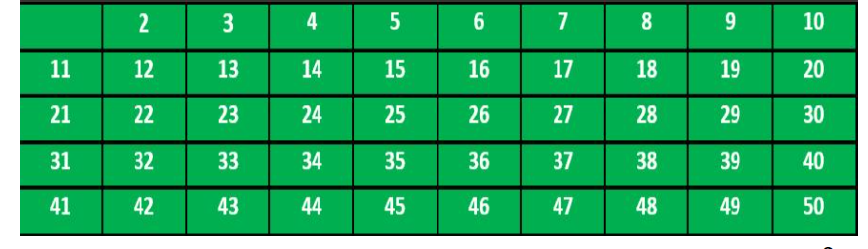
\includegraphics[width=340pt,height=120pt]{slike/sieve-it-0.png}
%\end{figure}

\begin{table}[H]
	\centering
	\begin{tabular}{|c|c|c|c|c|c|c|c|c|c|c} \hline
       & 2 & 3 & 4 & 5 & 6 & 7 & 8 & 9 & 10 \\ \hline
    11 & 12 & 13 & 14 & 15 & 16 & 17 & 18 & 19 & 20 \\ \hline
    21 & 22 & 23 & 24 & 25 & 26 & 27 & 28 & 29 & 30 \\ \hline
    31 & 32 & 33 & 34 & 35 & 36 & 37 & 38 & 39 & 40 \\ \hline
    41 & 42 & 43 & 44 & 45 & 46 & 47 & 48 & 49 & 50 \\ \hline     
	\end{tabular}
    \caption{Inicijalizacija.} \label{eratosten-sieve-it-0}
\end{table}


Dalje, u prvoj iteraciji, nalazimo se na poziciji 2, gdje elemente na pozicijama $2 \cdot k, k=2, \ldots, 50$ eliminišemo kroz sito (kao oni koji nisu prosti, dodijeljujući im vrijednost \emph{False}). Vizuelno, preostali brojevi za ispitivanje su oni neoznačeni:


%\begin{figure}[H]
%	\centering
%	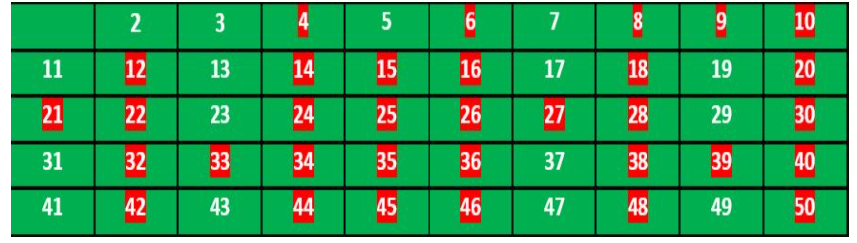
\includegraphics[width=340pt,height=120pt]{slike/sieve-it-1.png}
%\end{figure}

\begin{table}[H]
	\centering
	\begin{tabular}{|c|c|c|c|c|c|c|c|c|c|c} \hline
		& 2 & 3 & \cellcolor{red!30}  4 & 5 & \cellcolor{red!30} 6 & 7 & \cellcolor{red!30} 8 & 9 & \cellcolor{red!30} 10 \\ \hline
		11 &\cellcolor{red!30}  12 & 13 & \cellcolor{red!30} 14 & 15 & \cellcolor{red!30} 16 & 17 & \cellcolor{red!30} \cellcolor{red!30} 18 & 19 & \cellcolor{red!30} \cellcolor{red!30} 20 \\ \hline
		21 & \cellcolor{red!30} 22 & 23 & \cellcolor{red!30} 24 & 25 & \cellcolor{red!30} 26 & 27 &\cellcolor{red!30}  28 & 29 & \cellcolor{red!30} \cellcolor{red!30} 30 \\ \hline
		31 & \cellcolor{red!30} 32 & 33 & \cellcolor{red!30} 34 & 35 & \cellcolor{red!30} 36 & 37 & \cellcolor{red!30} 38 & 39 & \cellcolor{red!30} 40 \\ \hline
		41 & \cellcolor{red!30} 42 & 43 & \cellcolor{red!30} 44 & 45 & \cellcolor{red!30} 46 & 47 &\cellcolor{red!30}  48 & 49 &\cellcolor{red!30}  50 \\ \hline     
	\end{tabular}
        \caption{Eratostenovo sito: iteracija 1.} \label{eratosten-sieve-it-1}
\end{table}



Dalje, u drugoj iteraciji, prelazimo na poziciju 3. Kako je ona označena sa \emph{True} (prost broj), elemente na pozicijama $3\cdot k, k=3, \ldots, 16$ eliminišemo kroz sito (jer nisu prosti). Prelostali brojevi za ispitivanje su oni neoznačeni u narednoj tabeli. 

%\begin{figure}[H]
%	\centering
%	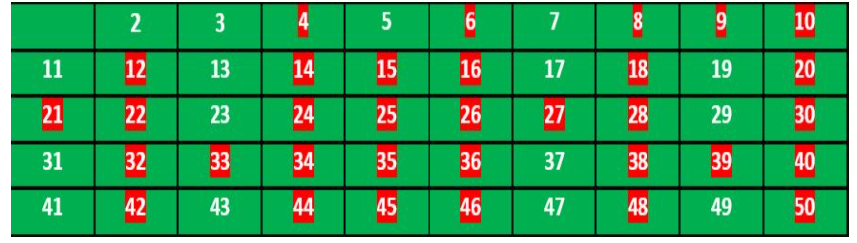
\includegraphics[width=340pt,height=120pt]{slike/sieve-it-1.png}
%\end{figure}

\begin{table}[H]
	\centering
	\begin{tabular}{|c|c|c|c|c|c|c|c|c|c|c} \hline
	& 2 & 3 & \cellcolor{red!30}  4 & 5 & \cellcolor{red!30} 6 & 7 & \cellcolor{red!30} 8 & \cellcolor{red!70} 9 & \cellcolor{red!30} 10 \\ \hline
	11 &\cellcolor{red!30}  12 & 13 & \cellcolor{red!30} 14 & \cellcolor{red!70} 15 & \cellcolor{red!30} 16 & 17 & \cellcolor{red!30} \cellcolor{red!30} 18 & 19 & \cellcolor{red!30} \cellcolor{red!30} 20 \\ \hline
	\cellcolor{red!70} 21 & \cellcolor{red!30} 22 & 23 & \cellcolor{red!30} 24 & 25 & \cellcolor{red!30} 26 & \cellcolor{red!70}  27 &\cellcolor{red!30}  28 & 29 & \cellcolor{red!30} \cellcolor{red!30} 30 \\ \hline
	31 & \cellcolor{red!30} 32 & \cellcolor{red!70} 33 & \cellcolor{red!30} 34 & 35 & \cellcolor{red!30} 36 & 37 & \cellcolor{red!30} 38 &  \cellcolor{red!70}   39 & \cellcolor{red!30} 40 \\ \hline
	41 & \cellcolor{red!30} 42 & 43 & \cellcolor{red!30} 44 & \cellcolor{red!70} 45 & \cellcolor{red!30} 46 & 47 &\cellcolor{red!30}  48 & 49 &\cellcolor{red!30}  50 \\ \hline     
\end{tabular}
        \caption{Eratostenovo sito: iteracija 2.} \label{eratosten-sieve-it-2}
\end{table}

U narednoj iteraciji prelazimo na poziciji 4. Kako to nije prost broj (dakle filtriran prethodno), prelazimo na naredni broj (5), koji je prost, nakon čega ponavljamo operacije opisane prethodnim iteracijama. 


\begin{table}[H]
	\centering
	\begin{tabular}{|c|c|c|c|c|c|c|c|c|c|c} \hline
		& 2 & 3 & \cellcolor{red!30}  4 & 5 & \cellcolor{red!30} 6 & 7 & \cellcolor{red!30} 8 & \cellcolor{red!30} 9 & \cellcolor{red!30} 10 \\ \hline
		11 &\cellcolor{red!30}  12 & 13 & \cellcolor{red!30} 14 & \cellcolor{red!30} 15 & \cellcolor{red!30} 16 & 17 & \cellcolor{red!30} \cellcolor{red!30} 18 & 19 & \cellcolor{red!30} \cellcolor{red!30} 20 \\ \hline
		\cellcolor{red!30} 21 & \cellcolor{red!30} 22 & 23 & \cellcolor{red!30} 24 & \cellcolor{red!90} 25 & \cellcolor{red!30} 26 & \cellcolor{red!30}  27 &\cellcolor{red!30}  28 & 29 & \cellcolor{red!30} \cellcolor{red!30} 30 \\ \hline
		31 & \cellcolor{red!30} 32 & \cellcolor{red!30} 33 & \cellcolor{red!30} 34 & \cellcolor{red!90} 35 & \cellcolor{red!30} 36 & 37 & \cellcolor{red!30} 38 & \cellcolor{red!30} 39 & \cellcolor{red!30} 40 \\ \hline
		41 & \cellcolor{red!30} 42 & 43 & \cellcolor{red!30} 44 & \cellcolor{red!30} 45 & \cellcolor{red!30} 46 & 47 &\cellcolor{red!30}  48 & 49 &\cellcolor{red!30}  50 \\ \hline     
	\end{tabular}
	\caption{Eratostenovo sito: iteracija 3.} \label{eratosten-sieve-it-3}
\end{table}

\section{Faktorizacija broja}

Fundamentalna teorema aritmetike kaže da se svaki prirodan broj $n>1$ može zapisati kao proizvod prostih brojeva na jedinstven način, do na redoslijed faktora. Drugim riječima, za svaki broj $n$ postoje prosti brojevi $p_1,p_2,\ldots,p_k$ i prirodni eksponenti $a_1,a_2,\ldots,a_k$ takvi da vrijedi $n=\prod_{i=1}^{k} p_i^{a_i}.$ Ovaj zapis naziva se \textit{prosta faktorizacija} broja $n$. Na primjer, $
120 = 2^3 \cdot 3 \cdot 5.$

\medskip

Sa algoritamskog stanovišta postavlja se pitanje kako efikasno odrediti prostu faktorizaciju datog broja. Naivan pristup podrazumijeva isprobavanje svih mogućih djelilaca, što za velike brojeve može biti veoma neefikasno.

Efikasniji pristup može se zasnovati na idejama korištenim u Eratostenovom situ. Osnovna ideja je sljedeća: za dati broj $n$ pronađemo njegov najmanji prosti djelilac $p$. Tada vrijedi $
n = p \cdot \frac{n}{p}.$ Nakon toga isti postupak rekurzivno primjenjujemo na broj $n/p$, sve dok ne dođemo do vrijednosti $1$. Na taj način broj postepeno razlažemo na proste faktore.

\medskip

Ovakav pristup prirodno slijedi paradigmu \textit{podijeli pa zavladaj}. Problem faktorizacije broja $n$ svodi se na faktorizaciju manjeg broja $n/p$, pri čemu se rezultat dobija dodavanjem prostog faktora $p$ u konačno rješenje.

\medskip

Da bi se postupak dodatno ubrzao, moguće je unaprijed konstruisati pomoćnu strukturu podataka koja za svaki broj $i$ čuva njegov najmanji prosti faktor. Ova struktura se može izgraditi modifikacijom Eratostenovog sita. Neka je niz $
SPF[0], SPF[1], \ldots, SPF[N]$ (eng. \emph{Smallest Prime Factor}) definisan tako da vrijednost $SPF[i]$ predstavlja najmanji prosti faktor broja $i$. Na primjer, $
SPF[12]=2,
SPF[15]=3,
SPF[49]=7.$ Za proste brojeve vrijedi $ SPF[p]=p. $

Nakon izgradnje niza $SPF$, faktorizacija broja $n$ postaje veoma jednostavna: u svakom koraku uzimamo vrijednost $SPF[n]$, dodajemo je u listu faktora i zamjenjujemo $n$ vrijednošću $
n \leftarrow \frac{n}{SPF[n]}.$

Postupak se ponavlja sve dok ne dobijemo $n=1$.

\medskip

Na primjer, za broj $120$ dobijamo: $
120 \rightarrow 60 \rightarrow 30 \rightarrow 15 \rightarrow 5 \rightarrow 1,$ odnosno proste faktore $2,2,2,3,5,$ što odgovara faktorizaciji $
120 = 2^3 \cdot 3 \cdot 5.$

\medskip

\textit{Kompleksnost algoritma.} Izgradnja niza najmanjih prostih faktora do granice $N$ može se izvršiti u vremenu reda $O(N \log \log N),$  dok se faktorizacija pojedinačnog broja $n$ izvršava u vremenu proporcionalnom broju njegovih prostih faktora, odnosno $O(\log n).$

Zbog toga je ovaj pristup naročito pogodan kada je potrebno faktorisati veliki broj različitih brojeva iz istog intervala.

 Implementacija ovakve (nizovne) strukture je data narednim k\^odom. 
 
 \begin{minted}{python}
 
   def sieve_adaptation(n):
   
       sieve_fact = [0] * (n+1)
       sieve_fact[0] = sieve_fact[1] = 0
       p = 2
       while p <= n:
           if sieve_fact[p] == 0:
       		  index = p * p
       		  while index <= n:
       			 sieve_fact[index] = p
       			 index += p
           p = p + 1
 	
	return sieve_fact
 	
   def factorization(n):
       
       factorize_min_p = sieve_fact(n)
       F = []
       while True: 
           i = factorize_min_p[n]
           if i == 0: 
              F.append(n)
              return F
           else:
              n = n // i
              F.append(i)
       return F  
   
   #ulaz: 
   n = 120
   F = factorization(n)
   print("Lista faktora je: ", F)
 \end{minted} 
 
\textit{Kompleksnost algoritma}. Najskuplja operacija u algoritmu je ada\-ptacija algoritma Eratostenovog sita (funkcija \texttt{sieve\_adaptation}) i ona se izvršava u $O(n \log \log n)$ vremenu. Glavna \texttt{while}-petlja se izvršava u linearnom $O(n)$ vremenu. Dakle, čitav algoritma se izvršava u 
 $O(n \log \log n)$ vremenu.
 
  \section{Izračunavanje binomnih koeficijenata} 
  
  Binomni koeficijenti igraju bitnu ulogu u kombinatorici. Npr. broj različitih grupa od $k$ ljudi može izabrati iz skupa od $n$ ljudi je predstavljen binomnim koeficijentom $\binom{n}{k}$. 
  
  \begin{definition}
  	 Binomni koeficijent $\binom{n}{k}$ gdje je $n, k \in \mathbb{N}, k > 0$  je dat sa 
  	 $$\binom{n}{k} = \frac{n(n-1) \cdots (n-k+1)}{k!}$$
  \end{definition}
  
~ pri čemu je $\binom{n}{0} := 1$. Binomni koeficijent $\binom{n}{1} = n,$ dok je $\binom{n}{n} = 1$ za sve $n \in \mathbb{N}.$ Takođe, ako je $n <k$, vrijedi $\binom{n}{k}=0$.
 
  Lako se može pokazati da vrijedi Paskalova jednakost:
  $$ \binom{n}{k} = \binom{n-1}{k-1} + \binom{n-1}{k},$$
   što nam daje rekurziju za računanje binomnih koeficijenta. Dakle, ako označimo $binom(n, k) = \binom{n}{k}$, vrijedi:
   $$ binom(n, k)= binom(n-1, k-1) + binom(n-1, k).$$
   
   Implementacija rekurzivnog pristupa je data sljedećim k\^odom.
   
   \begin{minted}{python}
     def binom(n, k): 
         if k == 0:
            return 1
         if n < k:
            return 0
         return binom(n-1, k-1) + binom(n-1, k)
   \end{minted}
  \textit{Kompleksnost algoritma}. Faktor grananja rekurzije je 2. To znači da na svakoj narednoj dubini rekurzije imamo (najviše) duplo više rekurzivnih poziva nego je to slučaj na dubini prije.  Kako je dubina rekurzije maksimalno $n$ (vrijednost prvog ili drugog atributa se smanjuje za 1 u narednom pozivu rekurzije), zaključujemo da je maksimalni broj poziva rekurzije eksponenci\-jalan i reda veličine $O(2^n)$. \\
  
  Optimizujmo ovu naivnu implementaciju rekurzije za računanje binomnih koeficijenata.  Jasno se vidi da se većina podproblema rješava više puta u rekurzivnim pozivima. Zbog toga ima smisla upotrebiti princip memoizacije. Označimo strukturu u kojoj čuvamo rješenja matricom $B[i][j]= \binom{i}{j}$. Bazni slučaj je  dat sa $B(n, 0) = 1 = B(n,n)$. Ako je $i < j$, tada je $B[i][j] = 0$. 
  
  Implementacija principa memoizacije za izračunavanje binomnog koefici\-jenta $\binom{n}{k}$ je data narednim k\^odom. 
  
  \begin{minted}{python}
  	
  	def initialization(n, k):
  	    Binom = [[-1] * (k+1)  for _ in range(n+1)] 
  	    return Binom 
  	    
  	def binom_memoization(i, j, Binom): 
  	    
  	    if Binom[i][j] != -1: # već računat
  	       return Binom[i][j] 
  	    if j == 0: 
  	       Binom[i][j] = 1
  	       return Binom[i][j] 
  	    if i < j: 
  	       Binom[i][j] = 0 
  	       return Binom[i][j]
  	       
  	    Binom[i][j] = binom_memoization(i-1, j-1, Binom) 
  	                + binom_memoization(i-1, j, Binom) 
  	    return Binom[i][j]

    #poziv metode:
    n = 10
    k = 4
    Binom = initialization(n, k) 
    n_over_k = binom_memoization(n, k, Binom) 
    print(n_over_k)
    
  \end{minted}  
  
  \textit{Kompleksnost algoritma}.  Kreiranje strukture se izvršava u $O(n\cdot k)$ vremenskoj kompleksnosti. Dalje,  broj podproblema koji se rješavaju je jednak $(n+1) \cdot (k+1)$.  U svakom rekurzivnom pozivu, izvršava se konstantan broj operacija. Sveukupno, kompleksnost algoritma je jednaka $O(n \cdot k)$. 
  
  
  
Katalanovi brojevi pojavljuju se u velikom broju interesantnih kombinatornih problema. U nastavku navodimo nekoliko njihovih poznatih interpretacija.

\begin{itemize}
	\item \textbf{Brojanje putanja na pravougaonoj mreži.} Broj različitih putanja od donjeg lijevog do gornjeg desnog ugla mreže dimenzija $n\times n$, pri čemu se u svakom koraku smije kretati samo udesno ili nagore, a putanja ne smije prelaziti iznad glavne dijagonale (može je samo dodirivati), jednak je $n$-tom Katalanovom broju.
	
	\begin{figure}[H]
		\centering
		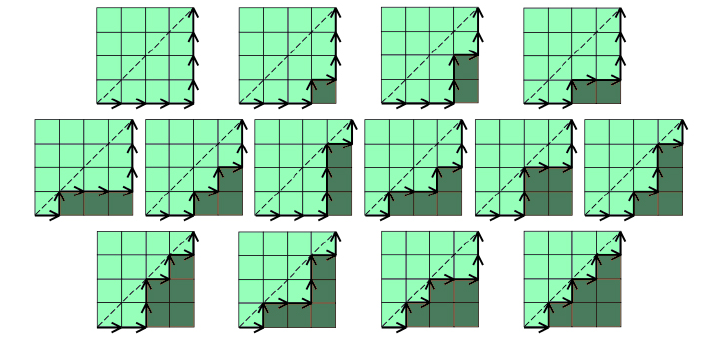
\includegraphics[width=280pt,height=160pt]{slike/catalan-net.png}
		\caption{Putanje na mreži dimenzija $4\times4$.}
		\label{fig:catalan-n-4}
	\end{figure}
	
	\item \textbf{Permutacije bez određenog paterna.} Broj permutacija skupa $\{1,2,\ldots,n\}$ koje ne sadrže patern \texttt{123} (ili, opštije, bilo koji fiksirani patern dužine $3$) takođe je dat Katalanovim brojevima. Na primjer, za $n=3$ dozvoljene su permutacije $	132, 213, 231, 312, 321,$
	dok permutacija \texttt{123} nije dozvoljena. Dakle, postoji ukupno $5$ takvih permutacija, što odgovara vrijednosti $C_3=5$.
	
	\item \textbf{Pravilno ugniježđene zagrade.} Katalanov broj $C_n$ predstavlja broj načina da se formira izraz sa $n$ parova zagrada tako da je svaka otvorena zagrada ispravno zatvorena. Na primjer, za $n=3$ postoji pet takvih izraza:$
	((())), (()()), (())(), ()(()), ()()().$
	
\end{itemize}

Prvih nekoliko Katalanovih brojeva su dati sa nizom: $
1, 1, 2, 5, 14,$ 42, 132, $429, 1430, 4862,\ldots$

Katalanovi brojevi zadovoljavaju sljedeću rekurzivnu relaciju: $
C(0)=1, $ i $
C(n+1)=\sum_{i=0}^{n} C(i),C(n-i),
\qquad n\geq 0.$

Ova rekurzija prirodno proizlazi iz činjenice da se mnogi objekti koji se broje Katalanovim brojevima mogu podijeliti na dva nezavisna dijela, čiji se doprinosi zatim množe i sabiraju preko svih mogućih podjela.

\medskip

Primijenimo sada paradigmu grube sile, odnosno direktnu rekurzivnu implementaciju, za računanje $n$-tog Katalanovog broja. Rekurzija slijedi neposredno iz prethodne formule:

\begin{minted}{python}
	def catalan(n):
	
	    if n == 0:
	        return 1
	        
	    result = 0
	    for i in range(n):
	        result += catalan(i) * catalan(n - 1 - i)
	return result
	
\end{minted}

\textit{Kompleksnost algoritma.} Ovakva implementacija generiše veliki broj ponovljenih izračunavanja istih podproblema. Zbog toga je njena vremenska složenost eksponencijalna. Upravo zbog izraženog preklapanja podproblema, računanje Katalanovih brojeva predstavlja prirodnu primjenu dinamičkog programiranja, koje značajno smanjuje vrijeme izvršavanja memoizacijom ili tabuliranjem prethodno izračunatih vrijednosti.
 Implementacija ovog pristupa je data sljedećim k\^odom. 
 
 \begin{minted}{python}
   def catalan(n):
       if n == 0:
          return 1
       catalan_n = 0 
       for i in range(n): 
           catalan_n += catalan(i) * catalan(n-1-i) 
       return catalan_n
        
 \end{minted}
  
  \emph{Kompleksnost algoritma}. Faktor grananja rekurzije je (najviše) $n$. Dubi\-na rekurzije je $n+1$. Dakle, kompleksnost ovog algoritma je eksponencijalna i iznosi $O(n^n)$. 

Optimizujmo ovaj naivni rekurzivni pristup za računanje Katalanovih brojeva. Kako je primijetno svaki podproblem izražunava iznova više puta, ponovo iskoristimo princip memoizacije. Čuvajmo vrijednost $i$-tog Katalano\-vog broja u nizovnoj strukturi $Cat(i)$.  Svojstvo optimalne podstrukture je dato rekurzijom $Cat(n+1) = \sum_{i=0}^{n} Cat(i) \cdot Cat(n-i).$ Bazni slučaj je dat sa $Cat(0) =1$.

Implementacija memoizacije je data sljedećim k\^odom.

  \begin{minted}{python}
	
	def initialization(n):
	   Cat = [ -1   for _ in range(n+1)  ] 
	   Cat[0]=1
	   return Cat 
	
	def catalan_i(i, Cat): 
	
	    if Cat[i] != -1:
	        return Cat[i]
     
            catalan_i = 0
            for k in range(i): 
                catalan_i += catalan_memoization(k, Cat) *
                     catalan_memoization(i-1-k, Cat)
    
            Cat[i] = catalan_i
            return Cat[i]
    
	#poziv metode:
	n = 10
	Cat = initialization(n) 
	
	cat_n = catalan_n(n, Cat) 
	print(cat_n)
\end{minted}  

\emph{Kompleksnost algoritma}. Dubina rekurzije je (najviše) $n+1$. U svakoj rekurziji, broj iteracija koji se izvršava je linearne kompleksnosti $O(n)$. Prema tome, kompleksnost algoritma je $O(n) \cdot O(n) = O(n^2)$.  \\


 % sretni brojevi, semi-prosti brojevi... 
 
 %Lucky numbers... 
 Posmatrajmo sljedeću proceduru konstruisanja niza brojeva.
 
 \begin{itemize}
 	\item Počinjemo od niza prirodnih brojeva
 	$1, 2, 3, 4, 5, 6, 7, 8$, $9, 10, 11$, $12, 13, 14, 15,$ $16, 17, 18, 19,\ldots 	$
 	
 	\item U prvom koraku brišemo svaki drugi broj. Dobija se niz $1, 3, 5, 7, 9,$ $11, 13, 15, 17, 19,\ldots$
 	
 	\item Iz novodobijenog niza zatim brišemo svaki treći broj, pa dobijamo $
 	1, 3, 7, 9, 13, 15, 19,\ldots
 	$
 	
 	\item Postupak se nastavlja tako što se iz trenutnog niza briše svaki četvrti broj, zatim svaki peti broj itd.
 	
 \end{itemize}
 
 Brojevi koji nikada ne budu obrisani nazivaju se \textit{srećnim brojevima} (eng. \textit{lucky numbers}).
 
 \medskip
 
 U ulazu je dat prirodan broj $n$. Potrebno je utvrditi da li je $n$ srećan broj, odnosno da li će preživjeti prethodno opisani proces eliminacije.
 
 \begin{solution}
 	
 	Posmatrajmo položaj broja $n$ tokom izvođenja postupka. U prvoj iteraciji briše se svaki drugi element niza. Prema tome, svi brojevi djeljivi sa $2$ bivaju uklonjeni.
 	
 	Ako je $n$ paran broj, zaključujemo da će biti obrisan već u prvom koraku i vraćamo rezultat \emph{False}. U suprotnom, broj $n$ preživljava ovu iteraciju. Pošto je uklonjena približno polovina elemenata, njegova nova pozicija postaje
 	
$$
 	n \leftarrow n - \left\lfloor \frac{n}{2} \right\rfloor .
$$
 	
 	U drugoj iteraciji briše se svaki treći element trenutnog niza. Ako je nova pozicija broja $n$ djeljiva sa $3$, broj se uklanja i vraća se rezultat \emph{False}. U suprotnom, broj ostaje u nizu, a njegova pozicija se ažurira na
 	
 	$$
 	n \leftarrow n - \left\lfloor \frac{n}{3} \right\rfloor.
 	$$
 	
 	Opštije, u $i$-toj iteraciji briše se svaki $(i+1)$-vi element trenutnog niza. Neka je trenutna pozicija posmatranog broja jednaka $n$.
 	
 	\begin{itemize}
 		\item Ako je $n < i+1$, broj više ne može biti obrisan ni u jednoj narednoj iteraciji, jer se uklanjaju samo elementi na pozicijama koje su višekratnici broja $i+1$. U tom slučaju vraćamo rezultat \emph{True}.
 		
 		\item Ako je $n$ djeljiv sa $i+1$, broj će biti obrisan u tekućoj iteraciji i vraćamo rezultat \emph{False}.
 		
 		\item U suprotnom, broj preživljava iteraciju, a njegova nova pozicija postaje
 		$$
 		n \leftarrow n - \left\lfloor \frac{n}{i+1} \right\rfloor ,
 		$$
 		jer se prije njega uklanja upravo
 		$\left\lfloor \frac{n}{i+1} \right\rfloor$
 		elemenata.

 		
 	\end{itemize}
 	
 	Postupak se ponavlja sve dok se ne utvrdi da je broj obrisan ili dok njegova trenutna pozicija ne postane manja od koraka eliminacije. U prvom slučaju broj nije srećan, dok u drugom zaključujemo da će preživjeti sve naredne iteracije i da jeste srećan broj.
 	
 \end{solution}
 
 
 Implementacija algoritma je data narednim k\^odom. 
 
 \begin{minted}{python}
 	from math import ceil
 	def lucky_number(n):
 
 	      
 	   for i in range(1, n): #iteracije
 	       if i+1 > ceil(n/i):
 	          return True 
 	       if ceil(n/i)  % (i+1) == 0:
 	          return False
 	   return True       
    
          #poziv funkcije
          print(lucky_number(7)) #True	       
  
 \end{minted}
  
 \end{solution}
 
 \section{Hornerov metod}
 
 \begin{definition}
 	\textbf{\textit{Hornerov metod za izračunavanje vrijednosti polinoma}}. Neka je dat polinom 
 	$P(x)=c_nx^n+c_{n-1}x^{n-1}+\cdots+c_1x+c_0,$ 
 	kao i tačka $x\in\mathbb{R}$. Potrebno je odrediti vrijednost polinoma $P$ u tački $x$. 
 	
 	Pretpostavimo da je polinom predstavljen nizom \texttt{coef}, pri čemu element \texttt{coef[i]} predstavlja koeficijent uz monom $x^{\,n-i}$, za $i\in\{0,\ldots,n\}$.
 	
 \end{definition}
 
 \begin{solution}
 	
 	Posmatrajmo primjer instance: $coef=[1,-3,2,-1], x=3.$ U ovom slučaju riječ je o polinomu $
 	P(x)=x^3-3x^2+2x-1.$ Vrijednost polinoma u tački $x=3$ iznosi $P(3)=27-27+6-1=5.$
 	
 	\medskip
 	
 	Naivan pristup podrazumijeva zasebno računanje svakog stepena $x^i$. Ako se vrijednost $x^i$ računa iterativno, potrebno je $O(i)$ operacija, pa ukupna vremenska složenost evaluacije polinoma iznosi $
 	O(1+2+\cdots+n)=O(n^2).$  	Hornerov metod omogućava izračunavanje vrijednosti polinoma u linearnom vremenu, odnosno u složenosti $O(n)$.
 	
 	Ideju algoritma ilustrujmo na prethodnom primjeru. Polinom možemo zapisati u obliku $P(x)=((x-3)x+2)x-1.$ Drugim riječima, $P(x)=(((c_3x+c_2)x+c_1)x+c_0).$
 	
 	Računanje se odvija sukcesivno:
 	
 	\begin{enumerate}
 		\item Počinje se od vodećeg koeficijenta $c_3=1$.
 		\item Trenutna vrijednost množi se sa $x=3$ i dodaje se naredni koeficijent: $1\cdot 3+(-3)=0.$
 		\item Dobijena vrijednost ponovo se množi sa $x$ i dodaje se sljedeći koeficijent: $ 0\cdot 3+2=2.$
 		\item Postupak se ponavlja: $2 \cdot 3+(-1)=5.$
 	\end{enumerate}
 	
 	Dobijamo konačnu vrijednost polinoma $	P(3)=5.$
 	
 	\medskip
 	
 	U opštem slučaju vrijedi identitet $$
 	c_nx^n+c_{n-1}x^{n-1}+\cdots+c_1x+c_0
 	=(\cdots((c_nx+c_{n-1})x+c_{n-2})x+\cdots+c_1)x+c_0.
 	$$
 	
 	Na ovaj način izbjegava se eksplicitno računanje stepena broja $x$, pa se polinom evaluira korištenjem samo $n$ množenja i $n$ sabiranja.
 	
 	\medskip
 	
 	\textit{Bazni slučaj}. Ako je $n=0$, polinom se svodi na konstantu $	P(x)=c_0,$ 	pa algoritam neposredno vraća vrijednost $c_0$.
 	
 	\medskip
 	
 	\textit{Kompleksnost algoritma}. Hornerov metod izvršava tačno $n$ množenja i $n$ sabiranja, pa je njegova vremenska složenost jednaka $
 	O(n),$	dok je prostorna složenost $O(1)$.
 \end{solution}
 
 Implementacija Hornerovog metoda je data narednim k\^odom. 
	 
	 \begin{minted}{python}
	 	 def horner_metod(coef, x):
	 	   
	 	     rezultat = 0
	 	     for c in coef:
	 	         rezultat = rezultat * x + c
	 	     
	 	     return rezultat
	 	 
	 	 # poziv funkcije
	 	 # Evaluacija:  x^3 - 3 x^2 + 2 x -1, x = 3
	 	 coef = [1, -3, 2, -1]
	 	 x = 3
	 	 print(horner_metod(coef, x))
	 \end{minted}

\textit{Kompleksnost algoritma.}  Jasno je da je najintenzivniji dio izvršavanja operacija smješten u \texttt{for}-petlju. Svaka iteracija se izvršava u konstantnom vremenu, pa zaključujemo da se algoritam izvršava u linearnom vremenu, tj. $O(n)$.  
\end{solution}
 
 %https://www.geeksforgeeks.org/sieve-of-atkin/ ==> SIEVE OF ATKIN ==> ako bude trebalo dodati...
 
 \section*{Zadaci}
 
 \begin{enumerate}
 	\item Broj je poluprost (eng. \textit{semiprime}) ako se može predstaviti
 	kao proizvod dva (ne obavezno različita) prosta broja. Npr. $4, 6, 9, 10, \ldots$ su neki od poluprostih brojeva. Konstruisati (efikasan) algoritam koji ispituje da li je broj poluprost.
 	\item Broj je savršen akko je jednak zbiru svojih djelilaca (ne računajući njega samog). Npr. 6 i 28 su savršeni jer je $6 = 1 + 2 + 3; 28 = 1 + 2 + 4 + 7 + 14$. Napisati program koji ispituje da li je broj savršen korištenjem Eratostenovog sita. Kolika je vremenska složenost algoritma? Uporediti ovaj algoritam sa algoritamskom paradigmom brutalne sile.
 	\item Broj je ružan akko su mu jedini prosti faktori 2 ili 3 ili 5. Niz prvih ružnih brojeva je dat sa $1, 2, 3, 4, 5, 6, 8, 9, 10, 12, 15, \ldots$ (1 je po
 	konvenciji uključen). U ulazu je  dat broj $n$. Izračunati $n$-ti ružni broj. Koristiti paradigmu dinamičkog programiranja.
 	\item Sfenički brojevi su pozitivni cijeli brojevi koji se dobijaju kao proizvod tačno 3 različita prosta faktora. Npr. $30, 42, 66, 70, 78,$ $102, 105, 110, 114, \ldots$ su neki od takvih brojeva. U ulazu je dat broj $n$. Ispitati da li je on sfenički? 
 	
 	\textit{Primjer}. $30=2 \cdot 3 \cdot 5$ jeste sfenički, dok $60 = 2^2 \cdot 3 \cdot 5 $ nije sfenički. 
 	\item Za broj se kaže da je slobodan od kvadrata ako ga nijedan
 	prosti faktor ne dijeli više od jednom, tj. najveći stepen prostog
 	faktora koji dijeli $n$  je jedan.  Prvih nekoliko slobodnih kvadrata brojeva su $$1, 2, 3, 5, 6, 7,
 	10, 11, 13, 14, 15, 17, 19, 21.$$   Na ulazu je dat broj $n$. Ispitati da li je on broj 	slobodnog kvadrata.
 	\item Neka je dat broj $n$. Ispitati da li je to \textit{lažni} broj ili ne.
 	Pod lažnim brojem podrazumijevamo složeni broj, čiji je zbir cifara jednak zbiru cifara njegovih različitih prostih faktora.%https://www.geeksforgeeks.org/hoax-number/
 	
 	\item Dat je skup od $n$ elemenata, pronaći broj načina particionisanja broja (Belovi brojevi). Implementirati efikasnu proceduru računanja ovakvih brojeva u zavisnosti od $n$.  %https://www.geeksforgeeks.org/bell-numbers-number-of-ways-to-partition-a-set/
 \end{enumerate}
\backmatter
% bibliography, glossary and index would go here.
\begin{thebibliography}{9}
	\bibitem{comen}
	T.Cormen, C. Leiserson, R. Rives, Introduction to algorithms, MIT Press, Cambridge, 2001.
	\bibitem{citekey}
	Ognjanovic, Zoran, and Nenad Krdzavac. "Uvod u teorijsko racunarstvo." Fakultet organizacionih nauka, Beograd (2004).
	\bibitem{ziv}
	Živković, Dejan. Uvod u algoritme i strukture podataka. Univerzitet Singidunum, 2010.
    \bibitem{zivkovic-algoritmi}
    Miodrag Živković. Algoritmi. Matematički fakultet, Beograd, 2000
    \bibitem{alg-design}
    Steven S. Skiena. The Algorithm Design Manual, Springer
    \bibitem{alg-design-2} Jeff Erickson. Algorithms, 2023
    
    \bibitem{unizg-algoritmi} Robert Manger, Miljenko Marušić. Strukture podataka i algoritmi (skripta).
    Prirodoslovno Matematiči Fakultet, Sveučilište u Zagrebu
    	\bibitem{geeks}
    https://www.geeksforgeeks.org
    \bibitem{link-zadaci}  {https://adriann.github.io/programming\_problems.html}
    \bibitem{ram-model}
    http://people.seas.harvard.edu/~cs125/fall14/lec6.pdf
    \bibitem{citekey} Horowitz E., Sahni S., Anderson-Freed S., Fundamentals of Data Structures in C. W.H. Freeman \& Co., New York, 1992.
\end{thebibliography}

\end{document}
